\documentclass[oneside,table]{tudelft-report}

% 1)Translates MATLAB code:
\usepackage[framed,numbered,autolinebreaks,useliterate]{mcode}
% enclose the MATLAB code by using begin/end{lstlisting}



% 2)Multiple figures on one page
\usepackage{float}
\usepackage[caption = false]{subfig}
\usepackage{color}

% 3)Own packages
\usepackage{graphicx}  %Used for figures
%\usepackage{subcaption} %Used for subcaptions
\usepackage{tabularx} %Used for tables to fit text width
\usepackage{adjustbox} %Used to keep tables within the page
\usepackage[justification=centering]{caption} %Used for the centering of the captions
\usepackage{multirow} %Allows for a table entry spanding multiple rows
\usepackage{longtable} %Allows for tables that cross multiple pages
%\usepackage{subcaption}
\usepackage{amsmath} %Used to make equations
%\usepackage{mathtools} %Used for more symbols for equations
\usepackage{gensymb} %Allows for the use of degree symbol and other generic symbols
\usepackage{enumitem} %Used to create custom lists...

\usepackage{afterpage} % Used for a blank page

\newcommand\blankpage{%
    \null
    \thispagestyle{empty}%
    \addtocounter{page}{-1}%
    \newpage}
%In the text before the blank page, insert the following code:

%\afterpage{\blankpage}    
    
    

\usepackage[intoc]{nomencl} \makenomenclature
\newcommand{\nomunit}[1]{%
\renewcommand{\nomentryend}{\hspace*{\fill}#1}}
%Used to make a nomenclature \nomenclature{$$}{\nomunit{$$}}
\usepackage{ifthen} % Used to create Roman and Greek list of symbols and order them


\renewcommand{\nomgroup}[1]{
 \ifthenelse{\equal{#1}{R}}{\item[\bfseries\sffamily\large{Roman}]}{
 \ifthenelse{\equal{#1}{G}}{\item[\bfseries\sffamily\large{Greek}]}{
 \ifthenelse{\equal{#1}{C}}{\item[\bfseries\sffamily\large{Constant}]}{
 \ifthenelse{\equal{#1}{S}}{\item[\bfseries\sffamily\large{Special}]}{}}{}}{}}
}

%\renewcommand{\nomgroup}[1]{
% \ifthenelse{\equal{#1}{R}}{\item[\bfseries\sffamily\large{Roman}]}{
% \ifthenelse{\equal{#1}{G}}{\item[\bfseries\sffamily\large{Greek}]}{}}
%}



%\usepackage[acronym]{glossaries}  %Used to crate a glossary, in this case list of abbreviations \newglossaryentry{}{name={}}{description={}}
%
%\newacronym{JPL}{name={JPL}}{description={Jet Propulsion Laboratory}}
%
%\makeglossaries
\usepackage[printonlyused]{acronym}  %Used to make the abbreviations list. Call = \ac{}

\newcommand{\acr}[1]{\acs{#1} (\aclu{#1})}
% Used to create a reversed acronym showing the abbreviaion first and then the full lenght meaning in brackets 

\usepackage{multicol} %Used to make multiple column text (for e.g. the list of abbreviations)

%\usepackage[ampersand]{easylist} %Used to make an easy list with different levels. But it doesn't look as cool as the normal nested list so I will not be using this package

\usepackage{tablefootnote} % Used to create footnotes in tables



\usepackage{bm} %Used to make capital greek letters bold in equations

\usepackage{xcolor} % Used to colour table cells. In cell use \cellcolor{red} to make it red. Use \cellcolor[gray]{0.9} to make it grey but only slighly lighter (90%). !!! Had to change \documentclass{tudelft-report} to \documentclass[table]{tudelft-report} for this to work!!!

%\usepackage{slashbox} % Used to make a diagonally shared cell for tables (maybe looks nice) use \backslashbox{}{} Update: looks terrible!



%\usepackage{diagbox} % Used to make a diagonally shared cell for tables (maybe looks nice) use \diagbox{}{} Update: doesn't make it to the lower corner...
%
%\usepackage{makecell} % Used to make a digonally shared cell for tables (maybe looks nice) use \diaghead{}%{}{} Update: nope, never mind....

\usepackage{hyperref} % Used to create links to websites
\urlstyle{same}


%\usepackage{cite} % I think this might let me select he references from a list whenever I type \cite. Awesome, it works :D. Update: nm, fucked everything up...

%\usepackage[authoryear]{natbib} % Used to cite in author-year instead of a number. Update: is already mentioned in the document class...

\allowdisplaybreaks

\usepackage{cleveref}
%use the \Cref command to reference instead and always have this package last!!

% 4)


\begin{document}

%\bibliographystyle{plain}

%% Use Roman numerals for the page numbers of the title pages and table of
%% contents.
\frontmatter

\title[Master Thesis]{Mars Sample Return Ascent Trajectory Analysis using Taylor Series Integration}
\author{S.D. \ Petrovi\'{c}}
\affiliation{Faculty Aerospace, Track Spaceflight}

\coverimage{cover_mars_4.jpg}
\makecover[backboxheight = 2.64in] %2.64in = 6.7056cm

 \afterpage{\blankpage}
%% Include an optional title page.
\begin{titlepage}

\begin{center}

%% Insert the TU Delft logo at the bottom of the page.
\begin{tikzpicture}[remember picture,overlay]
    \node at (current page.south)[anchor=south,inner sep=0pt]{
        
\includegraphics{cover/logo}
    };
\end{tikzpicture}

%% Extra whitespace at the top.
\vspace*{2\bigskipamount}

%% Print the title in cyan.
{\makeatletter
\titlestyle\color{tudelft-cyan}\Huge\@title
\makeatother}

%% Print the optional subtitle in black.
{\makeatletter
\ifx\@subtitle\undefined\else
    \bigskip
    \titlefont\titleshape\LARGE\@subtitle
\fi
\makeatother}

\bigskip
\bigskip

by
%door

\bigskip
\bigskip

%% Print the name of the author.
{\makeatletter
\titlefont\Large\bfseries\@author
\makeatother}

\vfill

in partial fulfillment of the requirements for the degree of
%in overeenstemming met de vereisten voor het verkrijgen van de graad van

\bigskip
\bigskip

{\bfseries Master of Science}

in Applied Physics

\bigskip
\bigskip

at the Delft University of Technology,
%aan de Technische Universiteit Delft,

to be defended publicly on Tuesday January 1, 2013 at 10:00 AM.
%in het openbaar de verdedigen op dinsdag 1 januari om 10:00 uur.

\vfill

\begin{tabular}{lll}
%% Add additional information here, per faculty requirements, e.g
%    Student number: & 1234567 \\
%    Project duration: & \multicolumn{2}{l}{March 1, 2012 -- January 1, 2013} \\
    Supervisor: & Prof.\ dr.\ ir.\ A.\ Einstein \\
    Thesis committee:
        & Prof.\ dr.\ C.\ F.\ Xavier, & TU Delft \\
        & Dr.\ E.\ L.\ Brown, & TU Delft \\
        & Ir.\ M.\ Scott, & Acme Corporation
\end{tabular}

%% Only include the following lines if confidentiality is applicable.
\bigskip
\bigskip
\emph{This thesis is confidential and cannot be made public until December 31, 2013.}
%\emph{Op dit verslag is geheimhouding van toepassing tot en met 31 december 2013.}

\bigskip
\bigskip
An electronic version of this thesis is available at \url{http://repository.tudelft.nl/}.
%Een elektronische versie van dit verslag is beschikbaar op \url{http://repository.tudelft.nl/}.

\end{center}

\end{titlepage}


\afterpage{\blankpage}

\chapter*{Preface} 
% Last updated: 4-2-2016
% Updated for final thesis draft: 04-01-2017
\setheader{Preface}

Back in December 2013 Warren Gebbett gave a presentation on his work at the \ac{JPL} in Pasadena, California, USA and the opportunity for a new student to go and perform research at \ac{JPL}. At this point I sent in my application together with eight other students.  Then at the end of December I heard that I was invited for an interview in the first week of January 2014. In this interview it was concluded that I met all the requirements and that I was the perfect candidate to follow Warren up as the next student at \ac{JPL} with financial backing of Dutch Space (now Airbus Defence and Space, the Netherlands). Financial backing was also provided by the Stichting Prof.dr.ir. H.J. van der Maas Fonds (Aerospace Engineering Faculty, TU Delft) and the Stichting Universiteitsfonds Delft (TU Delft). Communication with \ac{JPL} was started in February 2014 and in March 2015 it was clear that I would be working for the Mars Program Formulation Office under the supervision of Roby Wilson (Inner Planet mission design group, NASA \ac{JPL}). He told me to focus on subjects that dealt with Mars missions. At that point I was doing my internship at DLR Bremen on Lunar rocket ascent and descent, which lasted till June 2015. When I came back to Delft me and my supervisors Erwin Mooij (rockets, trajectories, entry and descent, TU Delft) and Ron Noomen (mission design and orbit analysis, TU Delft) agreed that it would be best to perform a study on these Mars subjects to prepare for my visit to \ac{JPL} and to formulate proposal thesis topics. The first week at \ac{JPL} I presented these initial thesis topics to both people from the Inner planet mission design group and the Mars program formulation office. The next few weeks were spent choosing and refining one of these topics. And in the months that followed after a literature study was performed to determine the final thesis topic. In the beginning of 2016 I got the green light to start my thesis research and so the journey that would last slightly longer than I expected started. It was not easy, and I quickly realised that I had misjudged the amount of time I would need to actually get my code to work and fix all the mistakes that I made. Rewriting models and equations completely happened so often that I lost count. All of this caused a lot of mental strain which was not always easy to deal with. But with the continuous support of my family, my friends, all my supervisors and colleagues I was still able to keep hope and push on. I never give up. And even though the research was slower than I expected and a lot of compromised had to be made in the end I am still happy with the results and the amazing opportunity that was given to me. This is why I would personally like to thank my TU Delft supervisors Ron Noomen and Erwin Mooij, for always keeping faith and sticking with me till the end. They were never afraid to speak their mind which always made me stronger. I would also like to thank my supervisor at \ac{JPL}, Roby Wilson for the great support and help during my year long stay in his group. His input always made me critically thing about what I was doing and showed me a slightly different view from the academics that I was used to. \\
During my time abroad I often had some personal struggles as well, which is why I would like to thank my parents, Robert and Linda Petrovi\'{c} for both the financial and mental support that they were able to give me. I would also like to thank the Rutkowski family for hosting me for several periods during my stay in the US and for being my family away from home. \\
Without all of you this thesis research would never have become a reality, which is why I am glad to be able to present the research that I performed the past year in this report. 


\begin{flushright}
{\makeatletter\itshape
    \@author \\
    Edam, The Netherlands, January 2017
\makeatother}
\end{flushright}


\afterpage{\blankpage}

\chapter*{Abstract}
% Created: 25-02-2017
\label{ch:Abstract}
Mars Sample Return is a mission concept that has been proposed many times in the past two decades. It is currently still being investigated by different space agencies around the world. The proposal of the Jet Propulsion Laboratory has reached the phase where different elements of this mission concept have been approved and are currently in the design phase. The complete campaign architecture involves three different missions: the first mission will have the objective to collect samples and store them, the second mission will then collect these stored samples and launch them into an orbit around Mars and the third mission will collect the orbiting sample and bring it back to Earth. The first part and the final part are currently secondary objectives for the Mars 2020 and Mars 2022 missions respectively. However, the second mission has not yet reached the approved design phase. 

An important objective of this second mission is to launch the samples into an orbit around Mars. This can be done using a Mars Ascent Vehicle. For such a mission profile, the ascent trajectory has to be simulated during the pre-design phase. An integrator can be used to simulate a Martian ascent by propagating the state of the vehicle in time. Numerical integration methods can be used for such a simulation, however in recent years another integration method has shown potential in both orbital trajectory problems as well as (re)-entry problems. This method is called \acf{TSI} and is based on the propagation of the state using Taylor series. The effectiveness of this integration method for a Mars ascent scenario is tested against the \acf{RKF78} numerical integrator. Therefore the goal of this research is to determine the speed of convergence, the accuracy and the computational speed of both methods. 

Using a set of spherical kinetic and dynamic equations in the rotating frame of Mars, taking into account the gravitational acceleration, the aerodynamic drag and the vehicle thrust, a trajectory was computed utilizing both integrators. The \ac{TSI} method was both more accurate and had a faster speed of convergence, however in this research the computational speed was still slower than the \ac{RKF78} reference numerical integrator. 

\ac{TSI} does, however, show other advantages compared to \ac{RKF78} as well: far fewer function calls, theoretically unlimited order (an optimum of order 20 was determined), can readily handle discontinuities, no interpolation is required afterwards resulting in a theoretically unlimited resolution and it shows less variation in the number of evaluations as a function of the error tolerance. A major disadvantage though of \ac{TSI} is that it can take a long time to set it up since it requires all equations before starting the integration.

An analysis on the influence of different parameters on a Mars ascent trajectory was also analysed using \ac{TSI}. Parameters that influence the trajectory are: launch latitude, launch flight-path angle and launch heading angle.

It can be concluded that \ac{TSI} is a viable integration method for use in ascent problems considering the rapid convergence and the accuracy of the results.


\afterpage{\blankpage}

\tableofcontents %Crates a table of contents
\afterpage{\blankpage}
%\listoffigures %Creates a list of figures

%\listoftables %Creates a list of tables

\clearpage
\markboth{Nomenclature}{Nomenclature}
%\addcontentsline{toc}{chapter}{Nomenclature}
\printnomenclature %Create the Nomenclature
\afterpage{\blankpage}

% if nomenclature does not work anymore go to options/configure texmaker and type .nlo -s nomencl.ist -o %.nls -t %.nlg instead of .idx to make it work again. Otherwise see: https://youtu.be/Ss1XfsaAnfs for details

\clearpage
\addcontentsline{toc}{chapter}{Abbreviations}
\markboth{Abbreviations}{Abbreviations}
\chapter*{Abbreviations} % Last updated 26-1-2016
\label{ch:abbr}

\begin{multicols}{2}
\begin{acronym}[LONGEST]
\acro{AB4}{Adams-Bashforth 4$^{th}$ order}
\acro{AB6}{Adams-Bashforth 6$^{th}$ order}
\acro{ABM4}{Adams-Bashforth-Moulton 4$^{th}$ order}
\acro{ABM12}{Adams-Bashforth-Moulton 12$^{th}$ order}
\acro{ACS}{Attitude Control System}
\acro{ACT}{Advanced Concepts Team}
\acro{ATK}{Aliant Techsystems}
\acro{BF}{Body-fixed}
\acro{CM}{Command Module}
\acro{CNES}{Centre National d'\'{E}tudes Spatiales}
\acro{CNRS}{Centre National de la Recherche Scientifique}
\acro{CSM}{Command and Service Module}
\acro{DE}{Differential Evolution}
\acro{DGB}{Disk-Gap Band}
\acro{DLR}{German Aerospace Center (Deutsches Zentrum f\"{u}r Luft- und Raumfahrt)}
\acro{DOPRIN87}{Dormand-Prince 8$^{th}$ $\left(7^{th}\right)$ order}
\acro{EA}{Evolutionary Algorithm}
\acro{ECEF}{Earth-centred Earth-fixed}
\acro{ECI}{Earth-centred inertial}
\acro{EDL}{Entry, descent and landing}
\acro{EP}{Electric propulsion}
\acro{ESA}{European Space Agency}
\acro{EoM}{Equations of Motion}
\acro{FPB}{Aerodynamic (or flight-path) body}
\acro{GA}{Genetic Algorithm}
\acro{GEO}{Geostationary Earth Orbit}
\acro{GLOM}{Gross Lift-Off Mass}
\acro{GMT}{Greenwich Mean Time}
\acro{GPS}{Global Positioning System}
\acro{GRAM}{Global Reference Atmospheric Model}
\acro{GTO}{Geostationary Transfer Orbit}
\acro{IAD}{Inflatable Aerodynamic Decelerator}
\acro{ITAR}{International Traffic in Arms Regulations}
\acro{ISS}{International Space Station}
\acro{JPL}{Jet Propulsion Laboratory}
\acro{JVSRP}{JPL Visitor Student Research Program}
\acro{LAM}{Lunar Ascent Module}
\acro{LAV}{Lunar Ascent Vehicle}
\acro{LEO}{Low Earth Orbit}
\acro{LM}{Lunar Module}
\acro{MA}{Martian Ascent}
\acro{MAV}{Mars Ascent Vehicle}
\acro{MBH}{Monotonic Basin Hopping}
\acro{MCI}{Mars-centred inertial}
\acro{MCMF}{Mars-centred Mars-fixed}
\acro{MEE}{Modified Equinoctial Elements}
\acro{MOLA}{Mars Orbiter Laser Altimeter}
\acro{MPF}{Mars Pathfinder}
\acro{MPFO}{Mars Program Formulation Office}
\acro{MRO}{Mars Reconnaissance Orbiter}
\acro{MSL}{Mars Science Laboratory}
\acro{MSR}{Mars Sample Return}
\acro{N/A}{Not Available}
\acro{NAIF}{Navigation and Ancillary Information Facility}
\acro{OS}{Orbiting Sample}
\acro{OTIS}{Optimal Trajectories by Implicit Simulation}
\acro{PaGMO}{Parallel Global Multi-objective Optimizer}
\acro{PICA}{Phenolic Impregnated Carbon Ablator}
\acro{POST}{Program to Optimize Simulated Trajectories}
\acro{PSO}{Particle Swarm Optimisation}
\acro{RCS}{Reaction Control System}
\acro{RF}{Frame of Reference}
\acro{RHR}{Right-hand-rule}
\acro{RKF45}{Runge-Kutta-Fehlberg 4$^{th}$ $\left(5^{th}\right)$ order}
\acro{RKF78}{Runge-Kutta-Fehlberg 7$^{th}$ $\left(8^{th}\right)$ order}
\acro{RKF}{Runge-Kutta-Fehlberg}
\acro{RHA}{Rover Hazard Avoidance}
\acro{RK4}{Runge-Kutta 4$^{th}$ order}
\acro{RKN12}{Runge-Kutta-Nystr\"{o}m 12$^{th}$ order}
\acro{SA}{Simulated Annealing}
\acro{s/c}{Spacecraft}
\acro{SC14}{St\"{o}rmer-Cowell 14$^{th}$ order}
\acro{SCI}{Solar system (sun-centred) inertial}
\acro{SEP}{Solar Electric Propulsion}
\acro{SG}{Shampine-Gordon}
\acro{SLA}{SuperLight Ablative}
\acro{SM}{Service Module}
\acro{SNOPT}{Sparse Nonlinear Optimizer}
\acro{SPICE}{Spacecraft Planet Instrument C-Matrix Events}
\acro{SQP}{Sequential Quadratic Programming}
\acro{SRC}{Sample Return Capsule}
\acro{ToF}{Time of Flight}
\acro{TOSCA}{Trajectory Optimisation and Simulation of Conventional and Advanced space transportation system}
\acro{TPS}{Thermal protection system}
\acro{TRW}{Thompson Ramo Wooldridge}
\acro{TSI}{Taylor Series integration}
\acro{Tudat}{TU Delft Astrodynamics Toolbox}
\acro{TVC}{Thrust Vector Control}
\acro{VCNE}{Vehicle-carried normal Earth}
\acro{VCNM}{Vehicle-carried normal Mars}


%\acro{}{}
%\acro{ACR}{Acronym}

\end{acronym}
\end{multicols} %Create the list of abbreviations
\afterpage{\blankpage}

%\printglossary[type=\acronymtype, title=Abbreviations] %Create a list of abbreviations


%% Use Arabic numerals for the page numbers of the chapters.
\mainmatter

\chapter{Introduction}  % Last updated: 4-2-2016 
\label{ch:intro}
\acf{MSR} has been a mission concept that has been proposed many times in the past two decades. Even today, research into this mission is still being done. And although it is not yet an official project proposal, NASAs \acf{JPL} is currently working on pre-cursor missions to eventually launch an \ac{MSR} mission. To prepare for this, research is being conducted on different aspects of \ac{MSR}, such as the \acf{MAV} responsible for transporting the dirt and soil samples into a Martian orbit and the orbiter which will then transport the samples back to Earth. The current orbiter proposed by \ac{JPL} is a low-thrust orbiter called Mars 2022. Such an \ac{MSR} mission requires precise and optimum (optimised for lowest \ac{GLOM}) trajectories to be able to bring back as many samples as possible. But how does one determine the optimum \ac{MAV} trajectory? Especially when it is combined with the optimum trajectory of the low-thrust orbiter. \\
The proposed research would focus on the combined optimisation of an \ac{MAV} trajectory and the trajectory of the low-thrust Mars 2022 orbiter. Also, one hypothesis is that great mass saving can be made if the orbiter and \ac{MAV} would rendezvous within one single orbital revolution after \ac{MAV} lift-off. Therefore, the question that should be answered is: what is the optimal trajectory solution for the combined trajectory problem of a high-thrust \ac{MAV} and a low-thrust Mars orbiter performing a single-revolution rendezvous in Mars orbit? More information on the proposed topic is provided in \Cref{ch:oversub}. \\
A mission such as \ac{MSR} and the corresponding trajectories can be described in many different reference frames, or \ac{RF}, and the motion of the \ac{MAV} and the orbiter can be modelled in different ways. Therefore it is important to use the proper equations and environmental models. Also, the trajectory has to be determined or rather a prediction will have to be made. This can be done using integration methods. And finally, the optimum will have to be found using an optimisation method. All these different aspects are addressed in this literature study.\\
First however, it is important to determine the knowledge that already exists and the research that has already been performed. Therefore, \Cref{ch:missher} will describe previous sample return missions, low-thrust \ac{s/c} missions, single-revolution rendezvous missions and the research performed in those fields. It will also describe the current \ac{MAV} designs. Then before mathematically representing the problem it is important to understand in what kind of \ac{RF} it has to be described. This will be done in \Cref{ch:reftrans}, followed by the \ac{MAV} ascent and low-thrust Mars 2022 orbiter model descriptions in \Cref{ch:launch,ch:transorb} respectively. Here, both chapters explain the assumptions and corresponding equations for each phase. One important aspect of the \ac{MAV} ascent, which sets it apart from other sample return missions, is that Mars has an atmosphere which cannot be neglected. Accordingly \Cref{ch:mars-atm-mod} describes the different atmospheric models and the trade-off that was performed to decide which model to use in this thesis problem. Then the integration and optimisation are discussed in \Cref{ch:int,ch:optimisation} respectively. In the integrators chapter, different integration methods are described and a selection is made of the integration methods that will be used. The same is done for the different optimisers. All of this information will be used to define the final thesis topic, which is presented in \Cref{ch:findef}. For some of the aspects that will be treated in the final thesis problem, certain software is already available. A summary of this software is provided in \Cref{ch:software}. Finally, a proposed schedule is presented in \Cref{ch:findef}, which shows the work which will have to be performed during the thesis work and the time that will have to be spend on each aspect of it. This literature study will serve as a guideline during the thesis project and provide background information for the final thesis report.

%This document has been written to provide a back-ground and better understanding of the preliminary thesis topic and the involved subjects that shall be used during the thesis work which will be performed at NASA \ac{JPL}. All the information gathered and provided in this report is used to finalise the thesis topic and formulate a final thesis proposal. The thesis work at \ac{JPL} is made possible through the \ac{JVSRP}, which has given the opportunity to do research at \ac{JPL} during a period of 1 year.
%The first few months were used to perform this literature study and the last months will be used to carry out the thesis research. During this entire period, the \ac{JPL} staff and resources have been set available to use for the research as long as it does not involve any restricted information or software. At the start of the research period it was known that the topic would involve a Mars mission. Because of restrictions and regulations it was decided that the thesis topic would include trajectory analysis and optimisation and the \ac{MSR} mission. Eventually, the initial topic was set on \ac{MSR} \ac{MAV} ascent trajectory and Mars 2022 orbiter trajectory combined optimisation to rendezvous in Mars orbit. The road-map towards and a more explicit explanation of the thesis topic will be explaine in \Cref{ch:oversub}. In \Cref{ch:missher} different reference missions and research for each aspect of the thesis topic are presented to get an idea of what has already been done and which missions and what research could be used for reference and validation. It is also very important to have a general idea about different mathematical concepts that will have to be used during the thesis work. For this purpose \Cref{ch:optimization} on optimisation and \Cref{ch:int} on integrators were written and form the basic understanding that is required. In the optimisation chapter, different optimisation methods are described and a selection is made of the optimisation methods that will be used. The same is done for the different integrators. The thesis problem will need to be described using mathematical model to simulate the ascent and orbital conditions of the \ac{MAV} and Mars 2022 orbiter respectively. \Cref{ch:launch} describes the used model, the assumptions and the corresponding equations for the ascent phase. In turn \Cref{ch:transorb} will describe the model, assumptions and equations for the orbiter. In these equations, many different reference frames and reference systems are used. This is why \Cref{ch:reftrans} describes the different required reference frames and systems and more importantly the transformation between these. All the required transformations, which follow from \Cref{ch:launch,ch:transorb}, are written out as well. One very important aspect of the \ac{MAV} ascent which sets it apart from other sample return missions is that Mars has an atmosphere which can not be neglected. This is why \Cref{ch:mars-atm-mod} describes the different models and the trade-off that was performed to decide which model will be best to use in this thesis problem. For some of the aspects that will have to be treated in the thesis problem, certain software is already available that can be used. A summary of this software is provided in \Cref{ch:software}. Finally, all the information gathered is used to produce a final thesis topic and corresponding proposed schedule which. The thesis proposal can be found in \Cref{ch:findef}. This entire document will be used during the thesis project and will serve as a guideline and provide background information for the final thesis report.


 		% Chapter 1


%\chapter{Overview} %Last updated 31-1-2016
\label{ch:oversub}

In \Cref{ch:intro} the initial topic was introduced: \acl{MSR} high-thrust ascent trajectory and low-thrust orbiter trajectory combined optimisation. Within this topic it is hypothesised that a rendezvous between the high-thrust \acf{MAV} and the low-thrust Mars 2022 orbiter in less than one revolution after \ac{MAV} launch would benefit both total mission mass and time. This initial topic is based on the proposed \acf{MSR} mission by \ac{JPL}\footnote{\label{foot:jpl_missions} All \ac{JPL} missions: \url{http://www.jpl.nasa.gov/missions/} [Accessed 30 July 2015]} and is interesting because of the many different aspects of this mission. It will involve the integration and optimisation of the ascent trajectory of the \ac{MAV} to low Mars orbit. Once in orbit, the \ac{MAV} will have to rendezvous with an orbiting \ac{s/c}. The current proposal involves the Mars 2022 orbiter, which will use a low-thrust propulsion system to manoeuvre in the Martian system and will initially be used to perform scientific measurements. The orbiter must then perform several orbit changes to position itself in the desired rendezvous orbit. This low-thrust trajectory will have to be integrated and optimised as well. At the start of this literature study it is proposed to combine these two trajectory optimisations in order to find the optimal total mission mass and time. The different aspects of this proposal will be investigated in this literature study to determine the different possibilities for Mars ascent trajectories, low-thrust orbital trajectories,  rendezvous in less than one revolution after launch, integration and optimisation of the trajectories. The final thesis proposal will be based on the information gathered and trade-offs perform in this study.




%\section{Searching for subjects}
%\label{sec:search}
%Since the thesis research is performed at NASA \ac{JPL} under their supervision it made sense to investigate the different missions that they have planned for the near future. An overview is provided on the \ac{JPL} website \footnote{\label{foot:jpl_missions} All \ac{JPL} missions: \url{http://www.jpl.nasa.gov/missions/}}. Two of the future and proposed missions to Mars were \ac{MSR} and Mars 2020. The \ac{MSR} mission is described as a mission that would return samples to Earth using a \ac{MAV} to launch from the Martian surface. The \ac{MAV} would contain rock, soil and atmospheric samples to be analysed back on Earth. The Mars 2020 mission (also sometimes referred to as the Mars Science Laboratory 2 mission) will be the next rover mission to Mars. Its prime goal will be to investigate the (past) habitability of Mars, and assess natural resources and possible hazards to help in the preparation of future human expeditions $^{\ref{foot:jpl_missions}}$. It is in its concept similar to the current Curiosity mission. Provided these two missions, it was then decided to formulate thesis subjects in correspondence with these missions but also correlate to personal preferences. This resulted in six thesis topics which were presented to \ac{JPL} after which the topic selection process was started. Together with the supervisors at the TU Delft and at \ac{JPL} it was decided to work out one of these topics in particular and write it into a proposal. Because the expertise of the section is on orbits it was decided to focus on \ac{MSR}, which also fits well with the current work of the \ac{MPFO} whom are designing the orbits for the Mars 2022 orbiter. The result is an initial thesis proposal that will be described in the next section.
%
%%As can be read in the next section, I was able to combine this into one topic. 
%
%%\section{Initial concepts}
%%\label{sec:inicon}
%%The first subject was based on the \ac{MSR} mission and incorporated the desire to work on both launcher trajectory and orbit optimisation. Therefore this subject was called \textbf{\textit{"Mars Sample Return launch trajectory"}}. 
%%
%%The goal would be to optimise the whole journey of the samples back to Earth starting with a Martian launch, then performing the transfer orbits to get it back to Earth, and finally re-entry to land the samples safely on Earth.\\
%%The second subject was based on the Mars 2020 mission and was mainly focussed on a Martian descent similar to the \ac{MSL} 1. This was interesting because the \ac{MSL} 1 mission had a very interesting descent phase consisting of several stages. The challenge here would be to see if this would be useful for a second mission as well, if so; where could it be improved. If not, what would be a better solution for Mars 2020 instead. This second subject was therefore called \textbf{\textit{"Mars Science Laboratory 2/Mars 2020 descent analysis"}}.\\
%%These were the initial subjects that were used during the early phases of the topic iteration process. This first iteration resulted in three thesis topics per corresponding subject. This was the result of some initial research into the subjects.
%%
%% These six topics were then presented to \ac{JPL} and the topic selection process was started. Together with the supervisors at the TU Delft and at \ac{JPL} it was decided to work out one of these topics in particular and write it into a proposal. Because the expertise of the section is on orbits it made more sense to go for \ac{MSR}, and this also fit well with the \ac{MPFO} since they want to design the orbits for the Mars 2022 orbiter. As can be read in the next section, I was able to combine this into one topic. 
%
%\section{Initial proposal}
%\label{sec:curprop}
%In this section the initial (starting) proposal is discussed based on the different aspects of a proposal as taught by the course Research Methodologies at the TU Delft. The initial working title is \textbf{\textit{"\acl{MSR} precise point rendezvous in Mars orbit}}. Please note that this is not the final proposal and will change due to the knowledge gained and provided in this literature study. 
%
%\subsection{Research objective}
%\label{subsec:resobj}
%The objective of this research is to find the optimum combination of the high-thrust \ac{MAV} launch trajectory and the orbital changes required for the low-thrust orbiter to rendezvous at a certain point above Mars, depending on the desired design choices, and returning the orbiter to a safe orbit by using \ac{TSI} to propagate the trajectories, Q-law to determine the low-thrust orbiter thrust curve and using \ac{DE} combined with and compared to \ac{MBH} to optimise for mass, \ac{ToF}, $\Delta V$,  $I_{sp}$ and/or $\theta$. 
%
%
%%\nomenclature{$ToF$}{Time of Flight\nomunit{s or days}}
%
%\subsection{Research perspective}
%\label{subsec:respers}
%It will be both Theory-testing research (\ac{TSI}, \ac{DE} and \ac{MBH}) and Problem-analysis research (optimum problem). The problem will be solved through the writing and validation of an optimisation program based on orbital mechanics and from a(n) (initial) mission design standpoint. It is therefore an engineering problem, and is a result of preliminary research and discussions between researchers, supervisors and stakeholders. 
%
%\subsection{Research framework}
%\label{subsec:resfram}
%The framework has been set-up based on the guidelines provided in Research Methodologies and the corresponding literature \cite{verschuren2010design} and is visualized in \Cref{fig:resframe}.
%
%\begin{figure}[!ht]
%\centering
%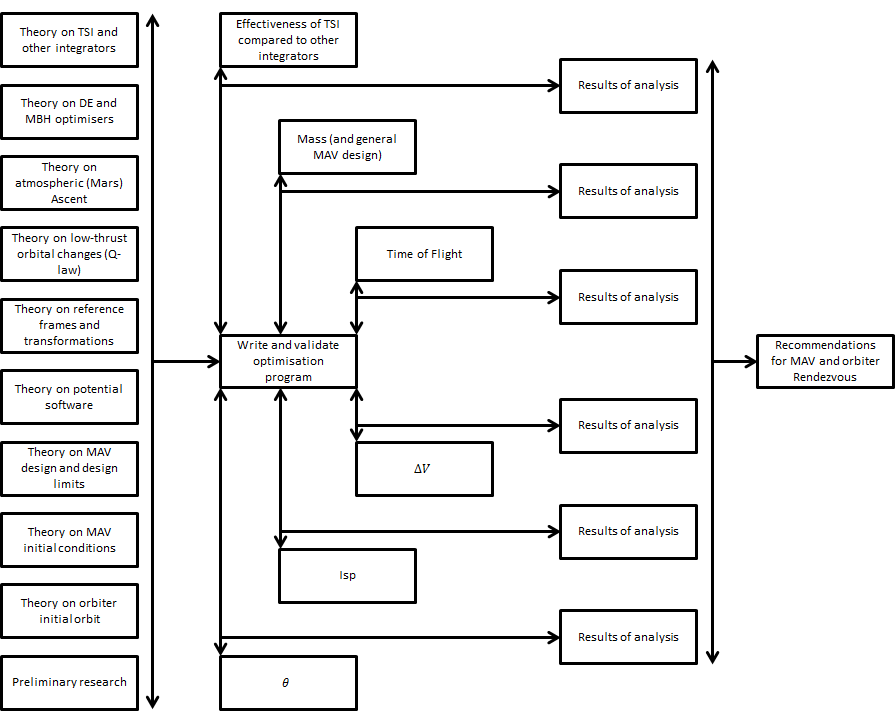
\includegraphics[width=0.9\textwidth]{figures/overview/resframe.png}
%\caption{Research framework for the literature study (a) and the thesis work (b, c \& d)}
%\label{fig:resframe}
%\end{figure}
%
%\textit{Formulation:} (a) the study of the different theories and the preliminary research will result in a model (b) that can be used to write and validate an optimisation program to optimise for the different parameters and also determine the usefulness of \ac{TSI}. (c) A comparison of the different optimisation results will help (d) establish the recommendations for the optimum \ac{MAV} and orbiter rendezvous above Mars.
%
%\subsection{Research questions}
%\label{subsec:resques}
%The corresponding research questions are listed:\\
%
%
%%\begin{easylist}
%%\ListProperties(Hide=100, Hang=true, Progressive=3ex, Style*=--,Style2*=$\circ$)
%%& What are the current integration and optimisation methods used to perform ascent and transfer trajectory optimisation, how are the proposed methods different, and what are the expected results?
%%&& What is the difference between \ac{TSI} and other frequently used integration methods in ascent and transfer trajectory calculations/optimisation and how do they work?
%%&& Which different optimisation methods are used in ascent and transfer trajectory optimisation and why have \ac{DE} and \ac{MBH} been chosen?
%%\end{easylist}
%
%\begin{itemize}
%\item What are the current integration and optimisation methods used to perform ascent and transfer trajectory optimisation, how are the proposed methods different, and what are the expected results?
%\begin{itemize}
%\item What is the difference between \ac{TSI} and other frequently used integration methods in ascent and transfer trajectory calculations/optimisation and how do they work?
%\item Which different optimisation methods are used in ascent and transfer trajectory optimisation and why have \ac{DE} and \ac{MBH} been chosen?
%\item What is the difference between \ac{DE} and \ac{MBH}, how do they work and what are the expected results?
%\item Which integration method(s) will \ac{TSI} be compared to, why these particular integration methods and what are the expected improvements of \ac{TSI} with respect to the other methods?
%\end{itemize}
%\item Which aspects, parameters and equations are involved when designing ascent and transfer trajectories, what is the underlying theory and how can it be applied here?
%\begin{itemize}
%\item What are the different aspects, parameters and equations when simulating an atmospheric ascent and how does that translate to Mars?
%\item How can a low-thrust orbit transfer be performed and optimised for a rendezvous in Mars orbit?
%\item Which perturbing bodies have to be accounted for in the Mars system to provide an accurate representation and which other perturbing sources have to be taken into account?
%\item Which frame(s) of reference will need to be used, and if more than one frame is required, how do they relate to each other?
%\item What will be the starting conditions of the \ac{MAV} and the orbiter?
%\item How do the different parameters affect the design of the \ac{MAV}, how much can it be changed and what are the design limits, and thus also parameter limits, for the \ac{MAV}?
%\item When aiming for an orbit using Q-law, how can a precise orbit position be incorporated?
%\end{itemize}
%\item What are the different optimal rendezvous situations given different design choices?
%\begin{itemize}
%\item How does the orbit of the orbiter have to change to reach the desired rendezvous point based on the design choices?
%\item What is the best \ac{MAV} configuration and combination of launch parameters to reach the desired rendezvous point based on the design choices?
%\item Which design is optimal for which design choice(s)?
%\end{itemize}
%\item Would \ac{TSI} be a good alternative for use in future optimisation programs?
%\begin{itemize}
%\item How much more (or less) accurate is \ac{TSI} compared to the other chosen integration methods?
%\item How much faster (or slower) is \ac{TSI} compared to the other chosen integration methods?
%\item What are the advantages and disadvantages (besides the first two sub-questions) when using \ac{TSI} in this kind of trajectory optimisation problem?
%\end{itemize}
%\item Which of the two (or what kind of combination of the two) optimisation methods worked best in this kind of trajectory optimisation problem, what are the advantages and disadvantages of the different methods? 
%\end{itemize}
%
%\subsection{Research strategy}
%\label{subsec:resstrat}
%The first step will be to perform a literature study on the subject, collect all the theory and become acquainted with this theory. The \ac{TSI} should be explained in detail as well as the chosen reference integration method. The same will have to be done for \ac{DE} and \ac{MBH} as well as the Q-law method. After completion of the literature study, the optimisation program will have to be written, using the \acl{TSI}, to optimise (utilizing both \ac{DE} and \ac{MBH}) Martian ascent to a certain parking/rendezvous orbit starting at different elevations, azimuth and launch angle with respect to the horizon. This would also be used to compare the \acl{TSI} with one (or a number of) other integration method(s), for a small number of orbits, to identify the most suitable integrator for this problem. Once this is completed, the program should be updated such that this ascent optimisation will be able to not just optimise to a certain parking/rendezvous orbit but to also get to a specific point in that orbit (include time and $\theta$) to perform a rendezvous manoeuvre with the orbiter. For the \ac{MAV} this means that it could either directly go to the rendezvous point or first into a parking orbit (starting on the Martian surface) and then to the rendezvous orbit and point. It is assumed that during the entire ascent and manoeuvring phase the \ac{MAV} uses a high-thrust propulsion system. As soon as this part of the program is validated, the orbiter can be added as well including Q-law. Given that the orbiter, which uses a low-thrust propulsion system, starts from a scientific orbit, optimise the rendezvous orbit and point such that both \ac{MAV} and orbiter will be at that point at the same time. After which the orbiter will have to go back to a higher orbit to avoid getting caught in the gravity well of Mars. During each stage of the program writing it will have to be verified and validated. The validation will be performed based on the results from current \ac{JPL} software used to perform orbit trajectory analyses and reference data from flown missions. Once the program validation has been completed, the actual optimisation process can commence and the optimisation will be performed for a number of different design choices while keeping within the limits of the \ac{MAV} design and the orbiter design. Finally, recommendations will be provided based on the different optimised results and design choices.
%
%\subsection{Research Method}
%\label{subsec:resmeth}
%The research will be performed using a self-written software program and validated with flight data and results from simulations performed with programs used by \ac{JPL}. 			% Not thesis

\chapter{Problem background} %Last updated 04-03-2016
\label{ch:problembackground}  % For thesis
\afterpage{\blankpage}

% Created 04-03-2016
% Put the atmospheric graph and drag coefficient graph fit in 19-09-2016
% 15-11-2016 add equations for state, state derivatives, gravity thrust and drag from early versions and used for RKF
% 17-11-2016 Remembered that I have to include a section on the cirularisation. And included the numbers for the speed of sound contant parameters.
% Updated 05-02-2017 implementation of feedback


\chapter{Models} 
\label{ch:models}
The \ac{MAV} and the corresponding ascent can be modelled in many different ways. Depending on the desired accuracy of the final solution compared to the real-life expected trajectory, different perturbations and freedom in motion can be defined and included, ranging from a low-fidelity (3DOF) to a high-fidelity program (6DOF). In a 3DOF system only the translational motion is taken into account, in 6DOF the rotational motion is also included, which makes it more accurate and more representative of a real-life scenario.

The main goal of this thesis is to determine if \ac{TSI} is an integrator that can be used for ascent cases and determine its performance compared to previously established methods. This comparison can be done with a less accurate representation of reality, because this allows for faster computations. Also, should the model be a 6DOF system, the extra accuracy would not have an added value because of all the errors in the assumptions made. Therefore a 3DOF system will suffice for the purposes of this research. In this 3DOF simulation the \ac{MAV} system can be modelled as a point-mass system with different accelerations acting on it. The change in position can be described by the kinematic equations and the change in velocity by the corresponding dynamic equations. The change in mass is described by the mass-flow. All these equations are provided in \Cref{sec:stateAndStateDerivatives}. For this model, three perturbing accelerations will be taken into account: gravity, thrust and atmospheric drag. The effect of third bodies can be neglected because of the short mission duration. All the accelerations are described in \Cref{sec:gravityModel,sec:thrustModel,sec:dragModel}, respectively. At the end of the integration, an impulsive shot is executed to circularise the orbit as described in \Cref{sec:modelCircularisation}.

\section{State And State Derivatives}
\label{sec:stateAndStateDerivatives}
%\textbf{\textcolor{red}{Maybe include more assumptions and corresponding explanations!!}}

In this research problem, different perturbations are best modelled in different reference frames. One example is the drag acceleration acting in the aerodynamic frame. However, the integration will be performed in the inertial frame. A collection of all the different frames required is shown in \Cref{fig:allFiveReferenceFrames_mooij2013fd-trinidad2012-mooij1994motion}.

\begin{figure}[H]
\centering
\subfloat[]{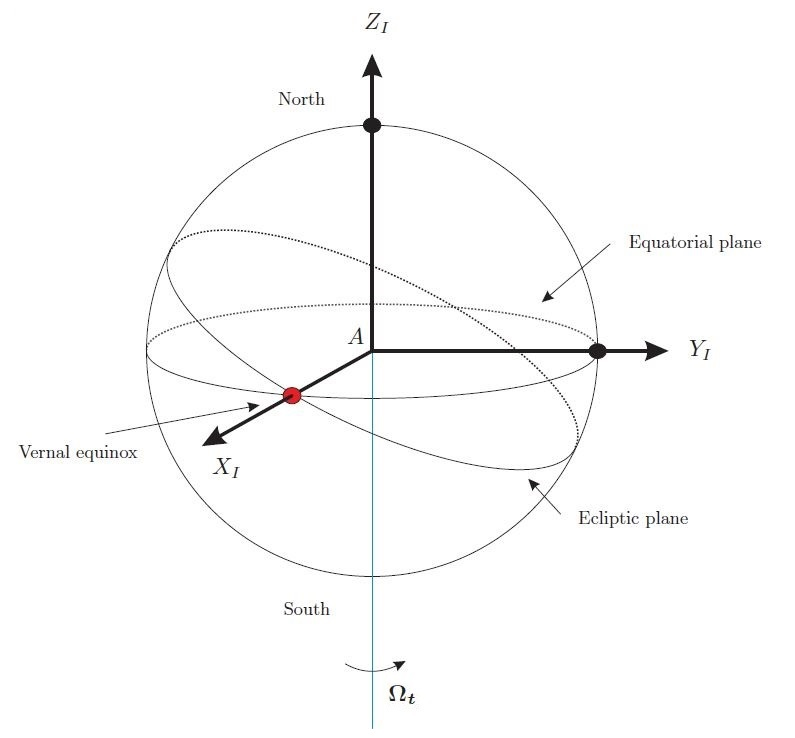
\includegraphics[width=0.5\textwidth]{figures/reference_frames/eci_mooij2013fd_noBox.jpg}\label{subfig:eci_mooij2013fd_noBox}} 
\subfloat[]{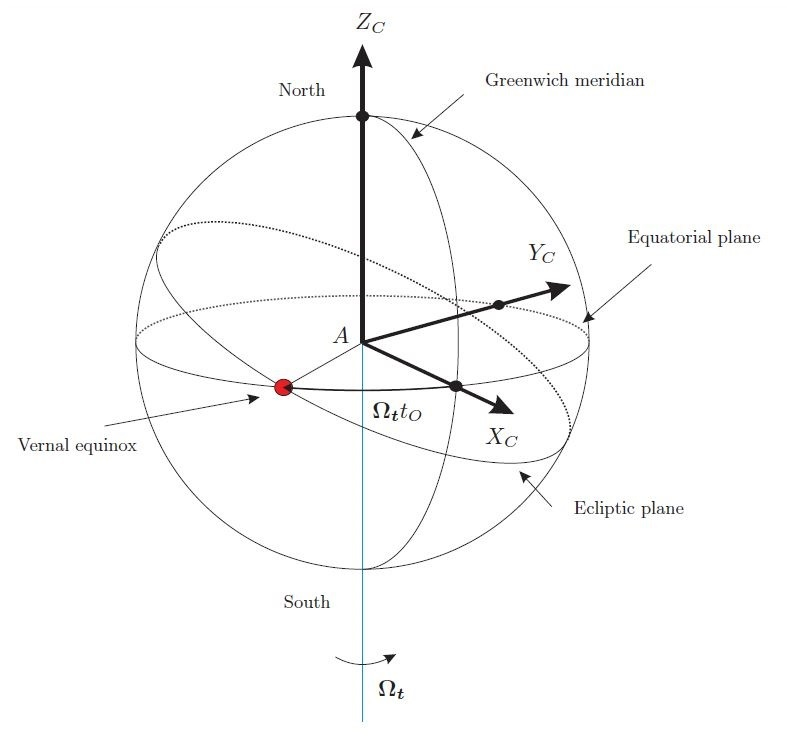
\includegraphics[width=0.5\textwidth]{figures/reference_frames/ecef_mooij2013fd_noBox.jpg} \label{subfig:ecef_mooij2013fd_noBox}}\\
 
\subfloat[]{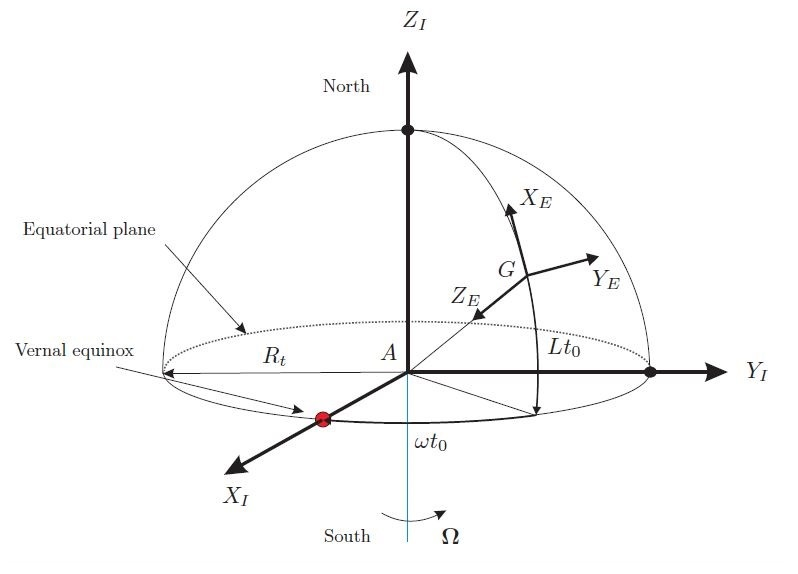
\includegraphics[width=0.5\textwidth]{figures/reference_frames/vcne_mooij2013fd_noBox.jpg}\label{subfig:vcne_mooij2013fd_noBox}} 
\subfloat[]{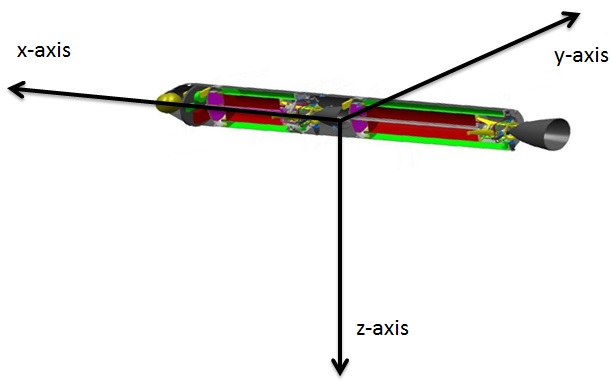
\includegraphics[width=0.5\textwidth]{figures/reference_frames/baseline_liquid_trinidad2012_bframe.jpg}\label{subfig:baseline_liquid_trinidad2012_bframe}}\\

\subfloat[]{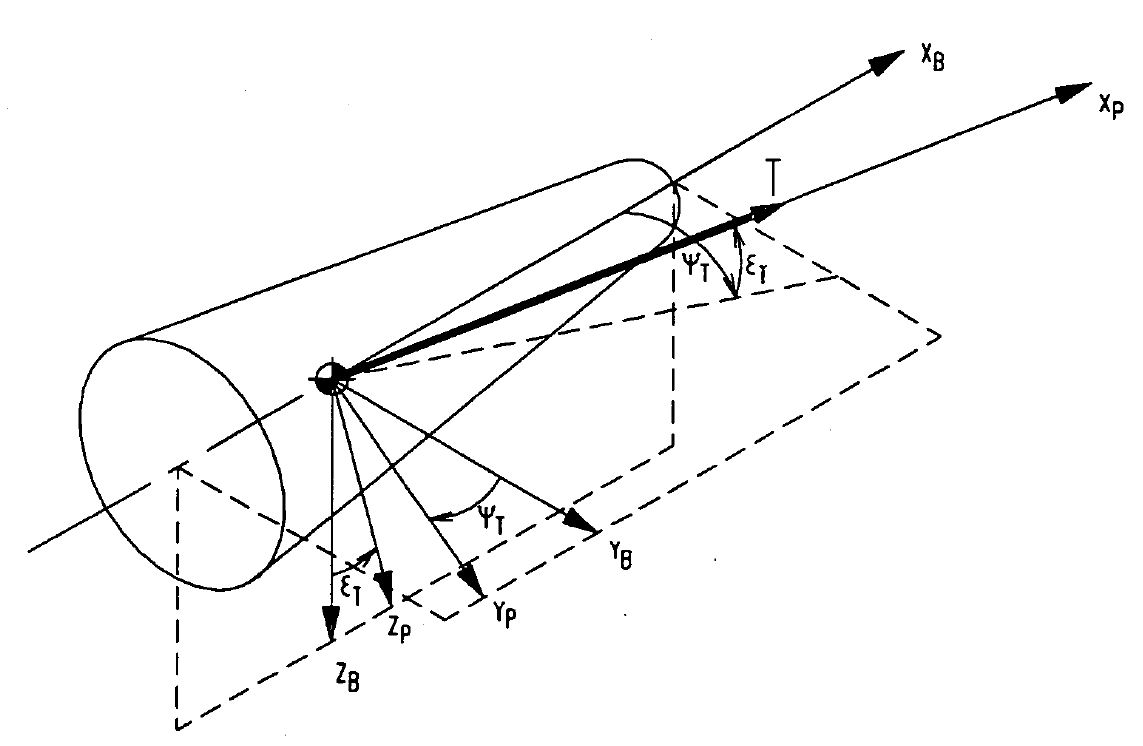
\includegraphics[width=0.5\textwidth]{figures/reference_frames/propframe_mooij1994motion.jpg}\label{subfig:propframe_mooij1994motion}}



\caption{Used reference frames \protect\subref{subfig:eci_mooij2013fd_noBox} (Mars centred) Inertial frame, \protect\subref{subfig:ecef_mooij2013fd_noBox} (Mars centred) Rotational frame, \protect\subref{subfig:vcne_mooij2013fd_noBox} (Vehicle centred) Vertical frame \citep{mooij2013fd}, \protect\subref{subfig:baseline_liquid_trinidad2012_bframe} (Vehicle centred) Body frame \citep{trinidad2012} and \protect\subref{subfig:propframe_mooij1994motion} (Vehicle centred) Propulsion frame \citep{mooij1994motion}. } 
\label{fig:allFiveReferenceFrames_mooij2013fd-trinidad2012-mooij1994motion} 
\end{figure} 


%\begin{figure}[H]
%\centering
%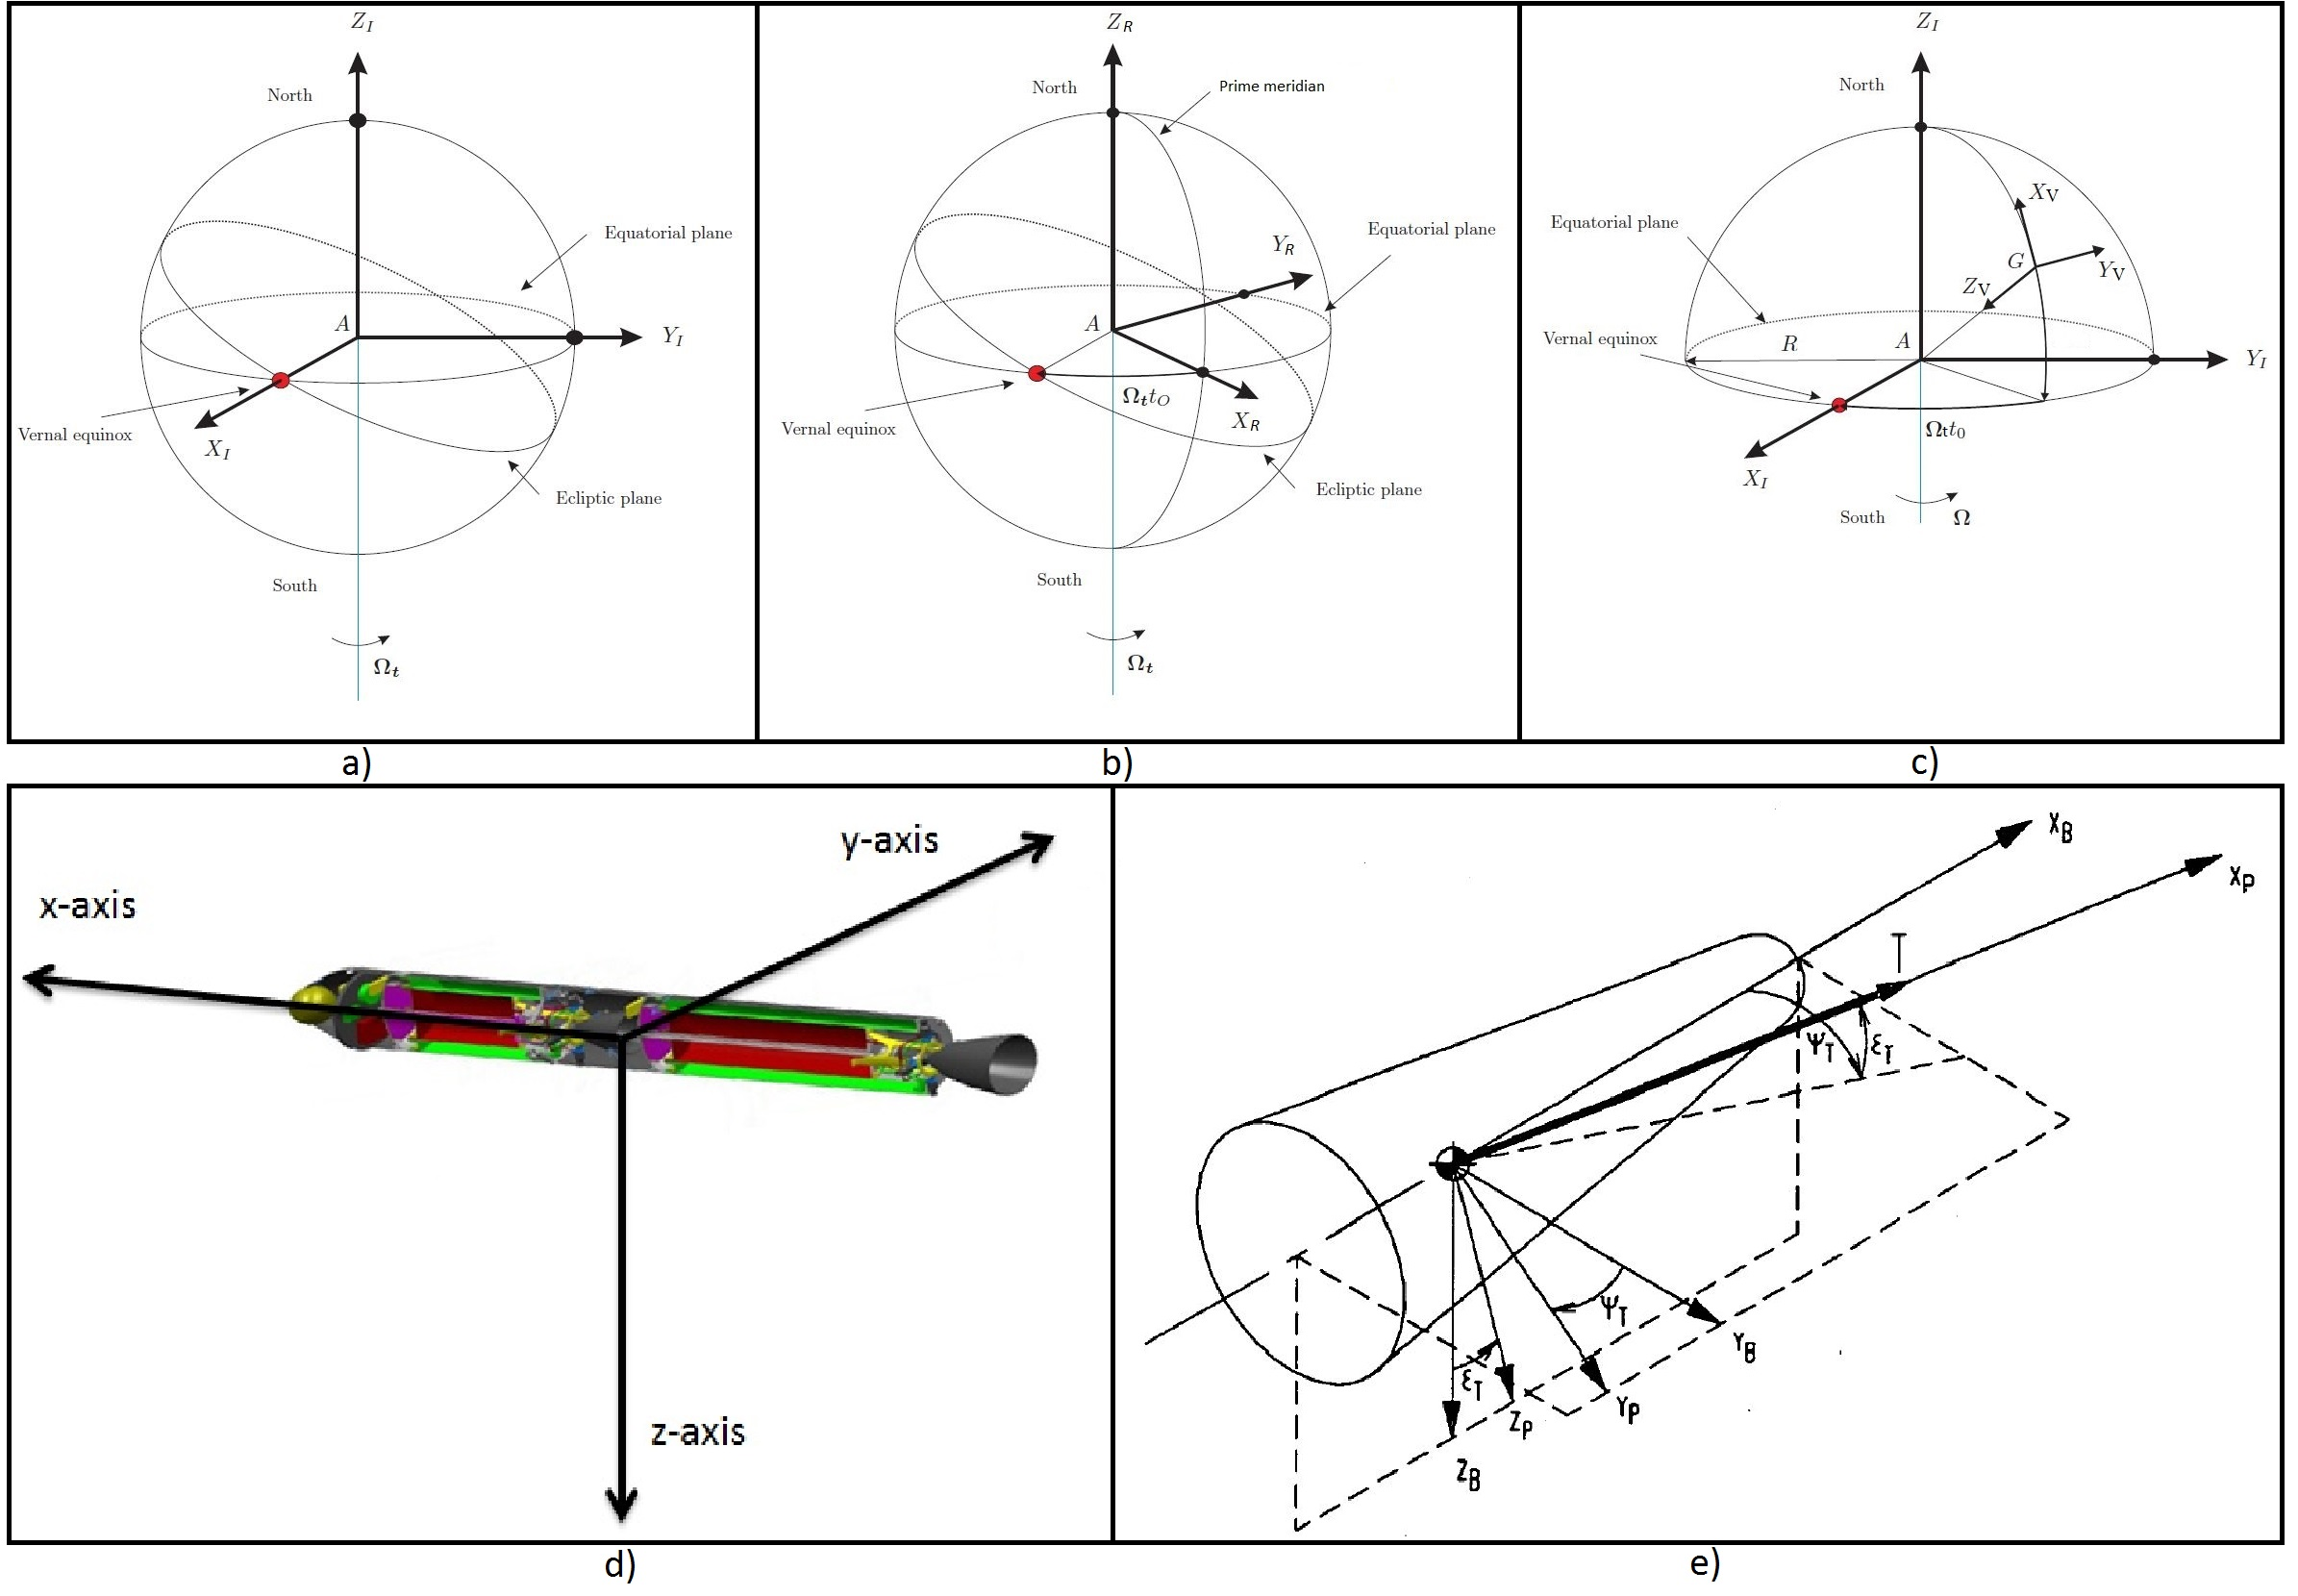
\includegraphics[width=1.0\textwidth]{figures/reference_frames/allFiveReferenceFrames_mooij2013fd-trinidad2012-mooij1994motion.jpg}
%\caption{a) (Mars centred) Inertial frame, b) (Mars centred) Rotational frame, c) (Vehicle centred) Vertical frame \citep{mooij2013fd}. d) (Vehicle centred) Body frame \citep{trinidad2012}. e) (Vehicle centred) Propulsion frame \citep{mooij1994motion}.}
%\label{fig:allFiveReferenceFrames_mooij2013fd-trinidad2012-mooij1994motion}
%\end{figure}

\noindent
This means that the accelerations have to be translated into the inertial frame through the presented frames. One way to do this is by using so-called transformation matrices ($\mathbb{T}$). These transformation matrices are composed of rotations around different axes over an associated angle $\phi$. An alternative would be to use quaternions instead, which make use of complex numbers. However, due to the workings of \ac{TSI} this was not easily implemented here which is why normal Euler angle transformations were used as the baseline for the rotation equations.  \Cref{fig:exampleXtrans_mooij2013stat} shows a general rotation around the x-axis. When this is set in a matrix, the transformation over the x-, y- and z-axis can be defined in the respective transformation matrices as described by \Cref{eq:allTransMatr}. 

\nomenclature[Rb0]{$\mathbb{T}$}{Transformation matrix \nomunit{-}}

\begin{figure}[!ht]
\centering
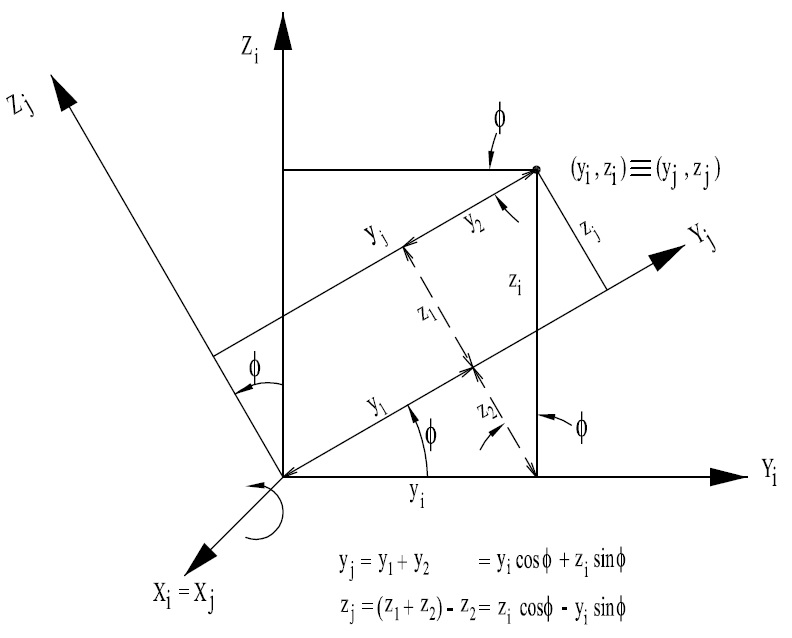
\includegraphics[width=0.5\textwidth]{figures/reference_frames/xtrans_mooij2013stat.jpg}
\caption{General rotation around the x-axis \citep{mooij2013stat}.}
\label{fig:exampleXtrans_mooij2013stat}
\end{figure}


\begin{equation} \label{eq:allTransMatr}
\mathbb{T}_{\mathbf{x}}(\phi)=\begin{bmatrix}
1 & 0 & 0 \\
0 & \cos\phi & \sin\phi \\
0 & -\sin\phi & \cos\phi \\
\end{bmatrix}, 
\mathbb{T}_{\mathbf{y}}(\phi)=\begin{bmatrix}
\cos\phi & 0 & -\sin\phi \\
0 & 1 & 0\\
\sin\phi & 0 & \cos\phi \\
\end{bmatrix}, 
\mathbb{T}_{\mathbf{z}}(\phi)=\begin{bmatrix}
\cos\phi & \sin\phi & 0\\
- \sin\phi & \cos\phi & 0\\
0 & 0 & 1\\
\end{bmatrix}
\end{equation}

\nomenclature[Ga4]{$\phi$}{General Euler angle \nomunit{rad}}

%More information on the different reference frames and the transformation matrices can be found in \Cref{app:appendixAA-referenceSystemTransformations}. \\
\noindent
Besides different reference frames, there are also different coordinate systems in which the state of a vehicle can be expressed. Three of the most used coordinate systems in space flight problems are the cartesian, spherical and keplerian system, and all of those systems (or formulations) are used in this research.\\ 
This also means that the state should be transformed between these different coordinate sets. In \Cref{fig:sphertocart_noomen2013basicFirst} it is shown how the position of a point can be described in either spherical coordinates or cartesian coordinates.


\begin{figure}[H]
\centering
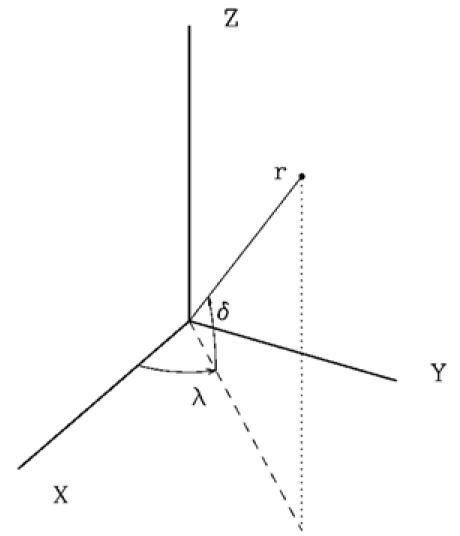
\includegraphics[width=0.3\textwidth]{figures/reference_frames/sphertocart_noomen2013basic.jpg}
\caption{Position expressed either in the cartesian (x,y,z) or in the spherical system ($r$, $\delta$, $\lambda$) \citep{noomen2013basic}.}
\label{fig:sphertocart_noomen2013basicFirst}
\end{figure}

\noindent
From this figure the relation can be described between the two different systems. This relation is important to allow for the translation between parameters expressed in one system to the other. More information on the transformations and coordinate system relations can be found in \Cref{app:appendixAA-referenceSystemTransformations}.
%
%If the cartesian coordinates are known, the spherical coordinates can be computed using \Cref{eq:cart2spher}.
%
%\begin{equation} \label{eq:cart2spher}
%\begin{split}
%r &= \sqrt{x^{2}+y^{2}+z^{2}}\\
%\delta &= \arcsin \left(\dfrac{z}{r}\right)\\
%\lambda &= \arctan \left(\dfrac{y}{x}\right)\\
%\end{split}
%\end{equation}

\nomenclature[Rb1]{$x$}{x-position coordinate \nomunit{m}}
\nomenclature[Rb5]{$y$}{y-position coordinate \nomunit{m}}
\nomenclature[Rb5]{$z$}{z-position coordinate \nomunit{m}}
\nomenclature[Ra5]{$r$}{Radius \nomunit{m}}
\nomenclature[Ga1]{$\delta$}{Latitude \nomunit{rad}}
\nomenclature[Ga3]{$\lambda$}{Inertial longitude \nomunit{rad}}

The general model is described in the Mars centred inertial frame in terms of the cartesian state (position and velocity in the x-, y-, and z-direction) and the mass. This is done because the cartesian state formulation in itself does not contain any singularities and will be used in the numerical integrator that will be compared to \ac{TSI}. However, different formulations based on the general model will be used for the propagation tool using \ac{TSI} as will be described in \Cref{ch:tsi}. The general cartesian notation is shown in \Cref{eq:stateModel}, where $m_{MAV}$ is the mass of the \ac{MAV} and the subscript $I$ refers to the inertial frame. This frame is used because the target orbit is a circular orbit around Mars described in the Mars centred inertial frame.

\begin{align} \label{eq:stateModel}
\mathbf{r}&=\begin{pmatrix}
x_{I}\\
y_{I}\\
z_{I}\\
\end{pmatrix}
&
\mathbf{V}&=\begin{pmatrix}
V_{x_{I}} \\
V_{y_{I}} \\
V_{z_{I}}\\
\end{pmatrix}
&
m_{MAV}&
\end{align}

\nomenclature[Rb0]{$V$}{Velocity \nomunit{m/s}}
\nomenclature[Ra4]{$m_{MAV}$}{\ac{MAV} mass \nomunit{kg}}


\noindent
To determine the next state, the change in the state parameters over time have to be computed. This is done by taking the time derivatives of the state as described by \Cref{eq:state_derivativesModel}.

\begin{align} \label{eq:state_derivativesModel}
\begin{split} 
\dot{x}_{I}&=V_{x_{I}}\\
\dot{y}_{I}&=V_{y_{I}}\\
\dot{z}_{I}&=V_{z_{I}}
\end{split} 
&
\begin{split}
\ddot{x}_{I}&=\dot{V}_{x_{I}}=a_{x_{I}}\\
\ddot{y}_{I}&=\dot{V}_{y_{I}}=a_{y_{I}}\\
\ddot{z}_{I}&=\dot{V}_{z_{I}}=a_{z_{I}}
\end{split}
&
\dot{m}_{MAV}=-\dfrac{T}{g_{0}I_{sp}}
\end{align}

\nomenclature[Ra0]{$a$}{Acceleration \nomunit{m/s$^{2}$}}
\nomenclature[Ca7]{$g_{0}$}{Standard gravitational acceleration at Earth sea level \nomunit{9.80665 m/s$^{2}$}}
\nomenclature[Ra8]{$T$}{Thrust \nomunit{N}}
\nomenclature[Ra2]{$I_{sp}$}{Specific impulse \nomunit{s}}



\noindent
From this point on, the subscript $I$ is omitted, because the state and the state derivatives are always presented in the inertial frame. If variables have to be presented in any other reference frame the corresponding subscripts will be provided and explained. The accelerations in the x-, y- and z-direction have three contributing components: gravitational acceleration, drag acceleration and thrust acceleration. In this model it is assumed that there is a homogeneous gravitational field acting on the point mass with a direction towards the centre of the inertial frame, which in this case is equal to the centre of Mars. The gravitational acceleration can therefore be directly expressed in the inertial frame. 

The drag is assumed to work in the opposite direction of the \ac{MAV} velocity vector, which in turn is assumed to be in the positive x-direction of the body frame associated with the \ac{MAV} (angle of attack and side-slip angle are assumed to be zero, so the aerodynamic frame is in this research the same as the body frame). Therefore the \ac{MAV} velocity, or ground velocity assuming there is no wind, is acting through the nose of the ascent vehicle. The drag acceleration is therefore expressed in the body frame. This effect in the body frame has to be translated into an acceleration in the inertial frame, which can be done using transformation matrices. A traditional transformation matrix uses an Euler angle to rotate a coordinate system in a certain reference frame to another. Using the proper Euler, or rotation, angles, the acceleration in the x-, y- and z-direction in the body frame can be transformed into acceleration components acting in the x-, y- and z-direction of the inertial frame. Once it is expressed in the inertial frame it can be added to the effect caused by the gravitational acceleration. 

It is also assumed that the nozzle of the \ac{MAV} engine can be pivoted in two different directions: the y-, and z-direction of the body frame using the thrust elevation angle $\epsilon_{T}$ and the thrust azimuth angle $\psi_{T}$. This means that the thrust acceleration can better be expressed in what is called the propulsion frame (see \Cref{subfig:propframe_mooij1994motion}). Because the nozzle can move in two directions, or rather pivot over two different angles, the thrust acceleration can be translated to the body frame using these two thrust angles. Once the thrust acceleration is expressed in the body frame, the same transformations that are used for the drag acceleration can be used to determine the thrust acceleration components in the inertial frame. \\

\noindent
Combining this in one equation then results in the expression for the acceleration vector as shown by \Cref{eq:accModel}. The subscript $G$ shows that the parameter is a function of the ground velocity, which in this case is equal to the velocity in the rotating frame of the \ac{MAV} itself because no wind is assumed. $\mathbb{T}$ stands for a transformation and the subscript determines the rotation axis. The parameter in the brackets for each transformation is the rotation angle, and each vertical line with a letter below it indicates the reference frame. 

\begin{multline} \label{eq:accModel}
\begin{pmatrix}
a_{x}\\
a_{y}\\
a_{z}\\
\end{pmatrix}
=
\begin{pmatrix}
a_{x,Grav}\\
a_{y,Grav}\\
a_{z,Grav}\\
\end{pmatrix}+
\Bigg|_{\mathbf{I}}\mathbb{T}_{\mathbf{z}}\left(-\Omega_{M}t_{O}+\omega_{P}\right)\Bigg|_{\mathbf{R}}\mathbb{T}_{\mathbf{z}}\left(-\tau\right)\mathbb{T}_{\mathbf{y}}\left(\dfrac{\pi}{2}+\delta\right)\Bigg|_{\mathbf{V}}\mathbb{T}_{\mathbf{z}}\left(-\chi_{G}\right)\mathbb{T}_{\mathbf{y}}\left(-\gamma_{G}\right)\Bigg|_{\mathbf{B}}\left[
\begin{pmatrix}
a_{Drag}\\
0\\
0\\
\end{pmatrix}
+  \right. \dots \\
\dotsc
 \left.
\Bigg|_{\mathbf{B}}\mathbb{T}_{\mathbf{z}}\left(-\psi_{T}\right)\mathbb{T}_{\mathbf{y}}\left(-\epsilon_{T}\right)\Bigg|_{\mathbf{P}}
\begin{pmatrix}
a_{Thrust}\\
0\\
0\\
\end{pmatrix}
\right]
\end{multline}

\nomenclature[Ca7]{$\Omega_{M}$}{Rotational velocity of Mars \nomunit{7.088$\cdot$10$^{-5}$ rad/s}}
\nomenclature[Ra7]{$t_{O}$}{Difference between current time and the inertial frame set time \nomunit{s}}
\nomenclature[Ga6]{$\omega_{P}$}{Off-set angle between inertial frame and zero meridian at inertial frame set time \nomunit{rad}}
\nomenclature[Ga4]{$\chi$}{Heading angle (or azimuth) \nomunit{rad}}
\nomenclature[Ga0]{$\gamma$}{Flight-path angle \nomunit{rad}}
\nomenclature[Ga3]{$\tau$}{Central-body fixed longitude \nomunit{rad}}
\nomenclature[Ga5]{$\psi_{T}$}{Thrust azimuth angle \nomunit{rad}}
\nomenclature[Ga2]{$\epsilon_{T}$}{Thrust elevation angle \nomunit{rad}}



\noindent
The rotations required to go from the body frame to the inertial frame are all a function of the current state. Both thrust angles are an input value that is set by the user or the program. $-\Omega_{M}t_{O}+\omega_{P}$ represents the angle between the rotating frame and the inertial frame and consists of three parts: $\Omega_{M}$ is the rotational velocity of Mars around its own axis, $t_{O}$ is the difference between the current time and the time at which the inertial frame was set on Mars, and $\omega_{P}$ is the angle between the x-axis of the inertial frame and the zero meridian at the time that the inertial frame was set on Mars. In this thesis the inertial frame is set at the beginning of the simulation (so at $t=0$, $t_{O}=0$) and is aligned with the rotating frame (so $\omega_{P}=0$). This means that the two reference frames shown in \Cref{subfig:eci_mooij2013fd_noBox,subfig:ecef_mooij2013fd_noBox} are alligned at the start of the simulation. The transformation from the vertical to the rotating frame requires the latitude and longitude of the \ac{MAV}, which is a function of the current state. \cite{mooij1994motion} provides equations to determine the different rotation angles. These expressions can be used to compute the latitude and longitude as well, as shown by \Cref{eq:latAndLong}.

\begin{align} \label{eq:latAndLong}
\begin{split} 
r&=\sqrt{x^{2}+y^{2}+z^{2}}\\
\delta&=\arcsin\left(\dfrac{z}{r}\right)
\end{split} 
&
\begin{split}
x_{R}&=\cos\left(\Omega_{M}t_{O}\right)x+\sin\left(\Omega_{M}t_{O}\right)y\\
y_{R}&=-\sin\left(\Omega_{M}t_{O}\right)x+\cos\left(\Omega_{M}t_{O}\right)y\\
\tau&=\text{atan2}\left(\dfrac{y_{R}}{x_{R}}\right)
\end{split}
\end{align}

\noindent 
It can be seen that to compute the longitude in the rotating frame ($\tau$) the position of the \ac{MAV} in the rotating frame is required. This position is found by transforming the inertial position to the rotational position using $\Omega_{M}t_{O}$ as described before. Working out that transformation matrix results in the sines and cosines presented in \Cref{eq:latAndLong}.\\

\noindent
Similarly, the flight-path angle $\gamma_{G}$ and the azimuth angle $\chi_{G}$ can be described as a function of the current state. For this, some intermediate parameters have to be computed first, which are given by \Cref{eq:intermediateParameters}. Here $V_{I}$ is the velocity in the inertial frame, $V_{G}$ is the velocity in the rotating frame and $V_{x,V}$, $V_{y,V}$ and $V_{z,V}$ are the respective x-, y- and z-velocity components in the vertical frame as depicted by \Cref{fig:vertical_spherical_mooij1994motion}.

\begin{equation} \label{eq:intermediateParameters}
\begin{split}
V_{I}=&\sqrt{V_{x}^{2}+V_{y}^{2}+V_{z}^{2}}\\
V_{G}=&\sqrt{V_{I}^{2}+\Omega_{M}^{2}\left(x^{2}+y^{2}\right)+2\Omega_{M}\left(xy-yx\right)}\\
V_{x,V}=&\left(V_{x}+\Omega_{M}y\right)\cdot \left(\sin\left(\delta\right)\sin\left(\Omega_{M}t_{O}\right)\sin\left(\tau\right)-\cos\left(\Omega_{M}t_{O}\right)\cos\left(\tau\right)\sin\left(\delta	\right)\right)+\\
&\left(V_{y}-\Omega_{M}x\right)\cdot \left(-\cos\left(\tau\right)\sin\left(\delta\right)\sin\left(\Omega_{M}t_{O}\right)-\cos\left(\Omega_{M}t_{O}\right)\sin\left(\delta\right)\sin\left(\tau\right)\right)+V_{z}\cos\left(\delta\right)\\
V_{y,V}=&\left(V_{x}+\Omega_{M}y\right)\cdot \left(-\cos\left(\tau\right)\sin\left(\Omega_{M}t_{O}\right)-\cos\left(\Omega_{M}t_{O}\right)\sin\left(\tau\right)\right)+\\
&\left(V_{y}-\Omega_{M}x\right)\cdot \left(\cos\left(\Omega_{M}t_{O}\right)\cos\left(\tau\right)-\sin\left(\Omega_{M}t_{O}\right)\sin\left(\tau\right)\right)\\
V_{z,V}=&\left(V_{x}+\Omega_{M}y\right)\cdot \left(\cos\left(\delta\right)\sin\left(\Omega_{M}t_{O}\right)\sin\left(\tau\right)-\cos\left(\Omega_{M}t_{O}\right)\cos\left(\tau\right)\cos\left(\delta	\right)\right)+\\
&\left(V_{y}-\Omega_{M}x\right)\cdot \left(-\cos\left(\tau\right)\cos\left(\delta\right)\sin\left(\Omega_{M}t_{O}\right)-\cos\left(\Omega_{M}t_{O}\right)\cos\left(\delta\right)\sin\left(\tau\right)\right)-V_{z}\sin\left(\delta\right)\\
\end{split}
\end{equation}

 \begin{figure}[H]
\centering
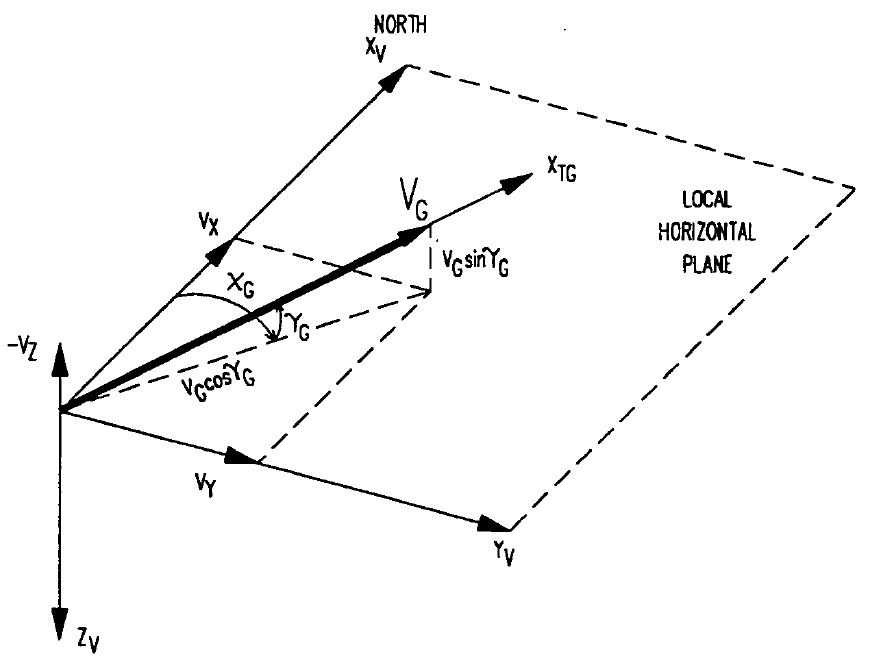
\includegraphics[width=0.5\textwidth]{figures/reference_frames/vertical_spherical_mooij1994motion.jpg}
\caption{Spherical velocity variables in a vertical cartesian frame \citep{mooij1994motion}.}
\label{fig:vertical_spherical_mooij1994motion}
\end{figure}

\noindent
Then the angles can be computed using these parameters as shown by \Cref{eq:fpaAndazimuth}.


\begin{equation} \label{eq:fpaAndazimuth}
\begin{split}
\chi_{G}&=\text{atan2}\left(\dfrac{V_{y,V}}{V_{x,V}}\right)\\
\gamma_{G}&=-\arcsin\left(\dfrac{V_{z,V}}{V_{G}}\right)\\
\end{split}
\end{equation}

\noindent
In this case, a transformation from the inertial frame to the vertical frame was required to get information on the velocity in the vertical frame. This transformation was written out in sines and cosines in \Cref{eq:intermediateParameters} resulting in lengthy expressions. \\

\noindent
Now that the rotation angles from the body frame to the inertial frame are known, only the thrust angles and the different accelerations have yet to be defined. This is done in the next sections.


\section{Gravity}
\label{sec:gravityModel}
The gravity acceleration is a function of the position of the \ac{MAV} and the standard gravitational parameter of the planet, in this case Mars. Often, irregularities in the mass distribution of a planet also have to be taken into account ($J_{2,0}$ etc.), however, because the mission time is very short and the \ac{MAV} does not even complete one revolution around Mars, these effects can be neglected. Therefore, the gravitational acceleration in the inertial frame can be represented by \Cref{eq:gravityModel}.

\begin{equation} \label{eq:gravityModel}
\begin{pmatrix}
a_{x,Grav}\\
a_{y,Grav}\\
a_{z,Grav}\\
\end{pmatrix}
=
\begin{pmatrix}
-\mu\dfrac{x}{r^{3}} \vspace{5pt} \\ \vspace{5pt} 
-\mu\dfrac{y}{r^{3}}\\
-\mu\dfrac{z}{r^{3}}\\
\end{pmatrix}
\end{equation}

% \vspace{5pt} is used to create vertical spacing between the different lines in the vector equation

%\nomenclature[Ca7]{$\mu_{M}$}{Mars standard gravitational parameter \nomunit{4.2828314$\cdot$10$^{-5}$km$^{3}$/s$^{2}$}}

\nomenclature[Ca7]{$\mu$}{Mars standard gravitational parameter \nomunit{4.2828314$\cdot$10$^{13}$m$^{3}$/s$^{2}$}}


\section{Thrust}
\label{sec:thrustModel}
The thrust acceleration in the propulsion frame is simply the thrust divided by the current mass of the \ac{MAV}, which can be written as shown by \Cref{eq:thrustModel}.

\begin{equation} \label{eq:thrustModel}
a_{Thrust}=\dfrac{T}{m_{MAV}}
\end{equation}

\noindent
However, this acceleration has to be transformed to the body frame using the thrust angles as defined in \Cref{subfig:propframe_mooij1994motion}. Both the thrust elevation as well as the thrust azimuth angle will be manually optimised to fit the trajectory and then set as a constant value during the entire ascent trajectory. They are thus not a function of the initial conditions but follow from the reference trajectory. The value for the thrust $T$ depends on the chosen \ac{MAV} design and can be different depending on the reference case. It will be set as a constant value during the ascent. 

%\begin{figure}[H]
%\centering
%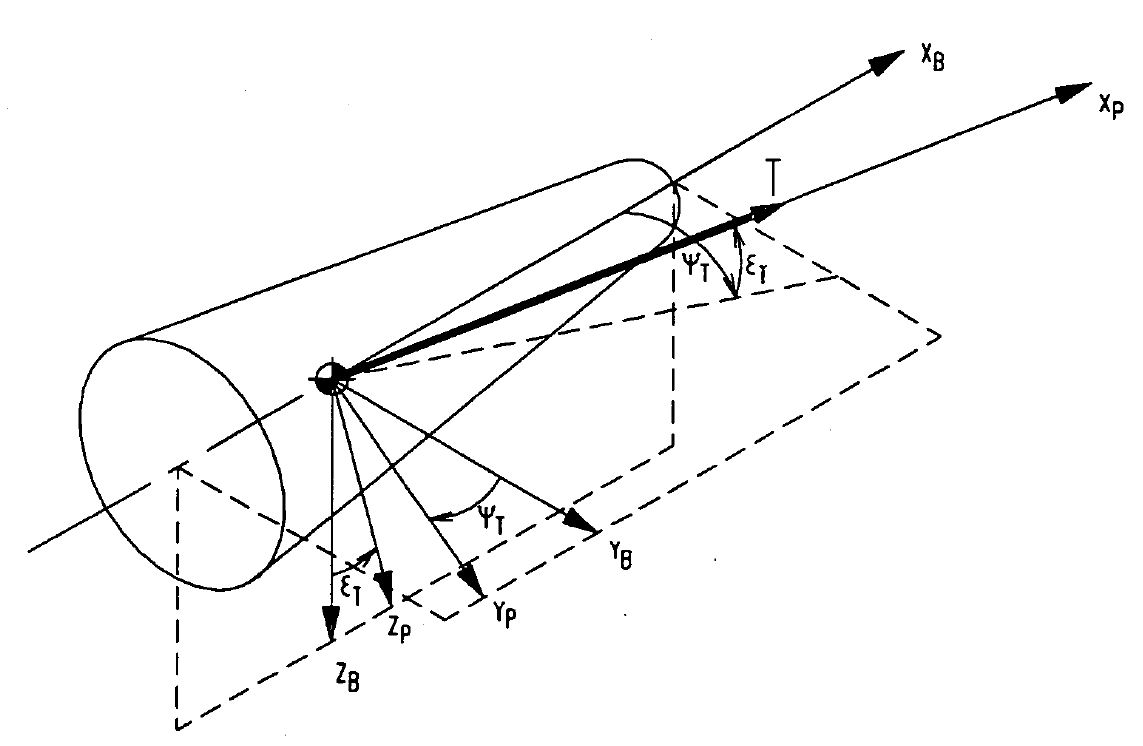
\includegraphics[width=0.5 \textwidth]{figures/reference_frames/propframe_mooij1994motion.jpg}
%\caption{Definition of the thrust elevation and thrust azimuth angle with respect to the body frame \citep{mooij1994motion}.}
%\label{fig:propframe_mooij1994motion}
%\end{figure}

\noindent
These angles will not be computed, but are set as an input for the program.


\section{Atmospheric Drag}
\label{sec:dragModel}
The drag acceleration can be represented similarly to the thrust acceleration taking into account that the drag is acting in the negative x-direction in the aerodynamic frame. The acceleration can then be written as \Cref{eq:dragModel}.

\begin{equation} \label{eq:dragModel}
a_{drag}=-\dfrac{D}{m_{MAV}}
\end{equation}

\nomenclature[Ra1]{$D$}{Drag \nomunit{N}}

\noindent
Here the drag is given by \Cref{eq:dragDragModel}, where the value for $V_{A}$ is in this case equal to $V_{G}$ because it is assumed that there is no wind.

\begin{equation} \label{eq:dragDragModel}
D=\dfrac{1}{2}\rho V_{A}^{2}SC_{D}
\end{equation}

\nomenclature[Ga3]{$\rho$}{Atmospheric density \nomunit{kg/m$^{3}$}}
\nomenclature[Ca7]{$S$}{Reference area \nomunit{0.091 m$^{2}$}}
\nomenclature[Ra1]{$C_{D}$}{Drag coefficient \nomunit{-}}

\noindent
Also, $S$ is the reference area of the \ac{MAV} set by the user, $\rho$ is the atmospheric density which is a function of the altitude $h\left(=r-R_{MOLA}\right)$ and $C_{D}$ is the drag coefficient of the \ac{MAV} which is a function of the Mach number. The Mach number in turn is a function of the speed of sound, which depends on the air temperature as can be seen in \Cref{eq:machAndSpeedOfSound}.

\nomenclature[Ca7]{$R_{MOLA}$}{Mars \acs{MOLA} reference radius (also $R_{M}$) \nomunit{3396$\cdot$10$^{3}$ m}}
\nomenclature[Ra1]{$h$}{Altitude \nomunit{m}}




 \begin{equation} \label{eq:machAndSpeedOfSound}
\begin{split}
M &= \dfrac{V_{A}}{a} \\
a &= \sqrt{\gamma_{a}R_{a}^{*}T_{a}} \quad \text{where} \quad R_{a}^{*}=\dfrac{R_{a}}{M_{a}} \\
\end{split}
\end{equation}

\nomenclature[Ra5]{$M$}{Mach number \nomunit{-}}
\nomenclature[Ra0]{$a$}{Speed of sound \nomunit{m/s}}
\nomenclature[Ca7]{$\gamma_{a}$}{Ratio of specific heats \nomunit{1.35}}
\nomenclature[Ca7]{$R_{a}$}{Molar gas constant \nomunit{8.3144598 m$^{2}$ kg s$^{-2}$ K$^{-1}$ mol$^{-1}$}}
\nomenclature[Ca7]{$M_{a}$}{Molecular mass of the Martian atmosphere \nomunit{0.04334 kg/mol}}
\nomenclature[Ra8]{$T_{a}$}{Atmospheric temperature \nomunit{K}}
\nomenclature[Ra6]{$R_{a}^{*}$}{Specific gas constant \nomunit{m$^{2}$ s$^{-2}$ K$^{-1}$}}
\nomenclature[Ra5]{$p_{n}$}{Polynomial coefficient \nomunit{-}}





\noindent
Here, $R_{a}$ is the molar gas constant, $\gamma_{a}$ is the ratio of specific heats for the Martian atmosphere, which according to \cite{ho2002radio} can be set to $\sim$1.35. $M_{a}$ is the molecular mass of the Martian atmosphere and depends on its composition. \cite{williams2015} mentions a volumetric composition of Mars which results in a mean molecular mass of 0.04334 kg/mol. This value has been used in this research to compute the Specific gas constant $R_{a}^{*}$.\\

\noindent
The temperature ($T_{{a}}$) change as a function of the altitude. This means that a temperature model of the atmosphere of Mars will have to be used to approximate these values as the ascent vehicle moves through the atmosphere. This is done through a function fit of an atmospheric model, as is described in \Cref{subsec:atmofuncfit}.\\

\noindent
The drag coefficient changes with the Mach number. Therefore, this also requires a function fit to be used in the simulation program. This fit is presented in \Cref{subsec:dragCoefFuncFit}.

\subsection{Atmospheric Density and Temperature Function Fit}
\label{subsec:atmofuncfit}
Several commercially available Mars atmospheric models are available that can be used to simulate the Martian atmosphere for use in, for instance, trajectory calculations. One of these models is the 2005 Mars-\acf{GRAM} \citep{justus1990mars} of which the 2005 version is free to use. This model is often used by the TU Delft and \ac{JPL} and has also been used by some of the reference research such as \cite{desai1998} and \cite{trinidad2012}.
Using Mars-\ac{GRAM} 2005, a table containing altitude, latitude and longitude dependent temperature and density data was produced. The altitude range was -0.6 to 320 km \acr{MOLA} with a step-size of 0.01 km, the latitude and longitude ranges were centred around the example launch site (21.0 $^\circ$N and 74.5 $^\circ$E) with a 10-degree range in each direction and a step-size of 1 degree. The rest of the input parameters were constant and can be seen in \Cref{app:appendixA-marsGRAM-inputFile}. The temperature and density data produced are shown in \Cref{fig:temperatureData,fig:densityData} respectively for nine latitude and longitude combinations including the reference launch site itself. This is therefore a sub-set of the full data volume available in Mars-\ac{GRAM} 2005.                                                                                                                                                                                                                                                                                                                                                                                                                                                                                          


\begin{figure}[H]
\centering
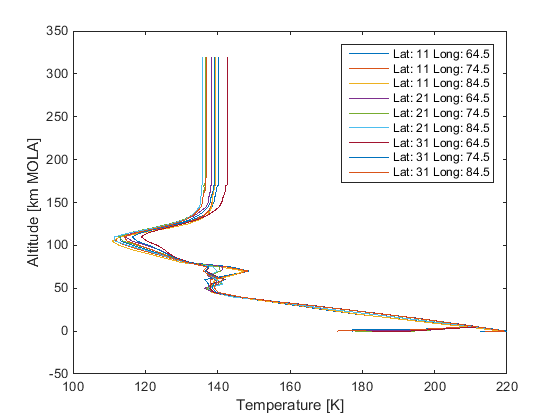
\includegraphics[width=0.7\textwidth]{figures/software/temperatureData.png}
\caption{Temperature data generated with Mars-\ac{GRAM} 2005 showing different latitude and longitude combinations.}
\label{fig:temperatureData}
\end{figure}

\begin{figure}[H]
\centering
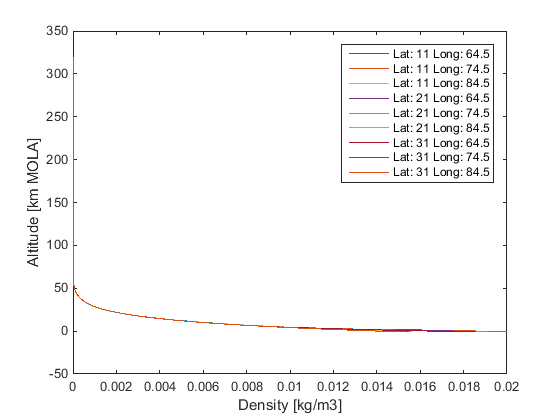
\includegraphics[width=0.7\textwidth]{figures/software/densityData.png}
\caption{Density data generated with Mars-\ac{GRAM} 2005 showing different latitude and longitude combinations.}
\label{fig:densityData}
\end{figure}

\noindent
Unfortunately, data tables cannot be used when integrating using \ac{TSI}, which is why both these data sets had to be fitted with differentiable functions. The temperature data cannot be fitted smoothly with one function.  Therefore, depending on the altitude range, a different approximation function is required. 

This calls for a polynomial function fitting for different sections of the temperature curve. Polynomial functions are easily differentiated and can be set-up with a large approximation precision of the curve section. The condition to be met for a proper fit came from the differences in the temperature-altitude and density-altitude curves, where the maximum difference with respect to the launch site curve was taken. The first requirement for the standard deviation of the polynomial curve fit was then to be (at least) one order lower than this maximum difference. The second requirement is that the maximum difference between the fit and the nominal launch site curve is lower than the initial maximum difference. The temperature-altitude curve was split into 5 sections as roughly visualised in \Cref{fig:temperatureDataSplit5}. The number of sections comes from both the shape of the curves and the requirement for accuracy and maximum order of the polynomial, which is set at 8 because otherwise the polynomial would get too long. This could result in longer run times and under-representation of certain parts of the curve. Also, the number of sections were to be kept at a minimum to avoid having to switch between too many sections slowing down the computation process. More information on the fitting process is provided in \Cref{app:appendixB-fittingProcessAndResults}.

\begin{figure}[H]
\centering
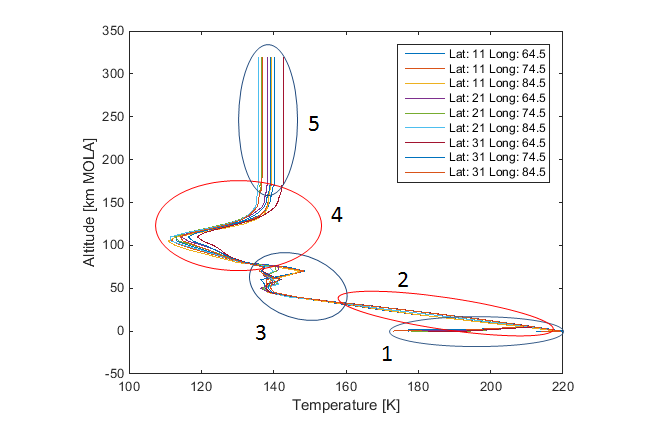
\includegraphics[width=1.0\textwidth]{figures/software/temperatureDataSplit5.png}
\caption{Different temperature curve sections.}
\label{fig:temperatureDataSplit5}
\end{figure}

\noindent
Each section was fitted with a polynomial function of order n as represented by \Cref{eq:polyGenFunct}. The last section shows a constant temperature, thus the temperature of the launch site curve was chosen to represent this final section, which is equal to 136.5 K.

\begin{equation} \label{eq:polyGenFunct}
y= p_{0}+p_{1}x+\dots+p_{n-1}x^{n-1}+p_{n}x^{n}
\end{equation}

\noindent
A low order is preferred, because then the fitted function will be simpler to evaluate and contain fewer terms. However the order has to be high enough to meet the accuracy requirements. To achieve this, the maximum difference between the data curves had to be higher than twice the maximum polynomial standard deviation to obtain approximately 95\% accuracy in the fit. \Cref{tab:fitDeviations} shows the orders that were required and the deviations to the launch site temperature-altitude curve. The actual corresponding parameters are provided in \Cref{tab:fitParameters}. It should be noted that the first few temperature data values were so different from the rest of the curve that it was assumed that this is due to uncertainty in the Mars-\ac{GRAM} program and were thus treated as outliers. The provided polynomial fit is only directly a function of the altitude, but because it is fit using different latitude and longitude curves it is indirectly also a function of the longitude and latitude variation. The complete polynomial fit for the launch site curve for the temperature is shown in \Cref{fig:completePolyFitTempSplit5}.

\begin{table}[H]
\begin{center}
\caption{Temperature curve fit data all with respect to the launch site curve (latitude and longitude of the launch site).}
\label{tab:fitDeviations}
\begin{tabularx}{1.0\textwidth}{|l|p{2.2cm}|l|X|X|X|}
\hline 
\small \textbf{Section} & \small \textbf{Altitude range [km MOLA]} & \small \textbf{Order}	& \small \textbf{Maximum polynomial standard deviation [K]} & \small \textbf{Maximum polynomial difference [K]} & \small \textbf{Maximum data curves difference [K]} \\ \hline 
1 & -0.6 to 5.04 & 1 & 0.0312 & 25.8 & 0.177 \\ \hline
2 & 5.04 to 35.53 & 2 & 0.287 & 3.90 & 0.7056 \\ \hline
3 & 35.53 to 75.07 & 6 & 0.624 & 8.00 & 1.69 \\ \hline
4 & 75.07 to 170.05 & 8 & 0.523 & 6.60 & 2.45 \\ \hline
5 & $>$ 170.05 & 0 & 0.0 & 5.5 & 5.5 \\ \hline
\end{tabularx}
\end{center}
\end{table}

\begin{table}[H]
\begin{center}
\caption{Temperature curve fit parameters (rounded to 3 decimal points)}
\label{tab:fitParameters}
\begin{tabular}{|l||p{1.1cm}|p{1.1cm}|p{1.1cm}|p{1.1cm}|p{1.1cm}|p{1.1cm}|p{1.1cm}|p{1.1cm}|p{1.1cm}|}
\hline 
\textbf{Section}  & $\mathbf{p_{0}}$ & $\mathbf{p_{1}}$ & $\mathbf{p_{2}}$ & $\mathbf{p_{3}}$ & $\mathbf{p_{4}}$ & $\mathbf{p_{5}}$ & $\mathbf{p_{6}}$ & $\mathbf{p_{7}}$ & $\mathbf{p_{8}}$ \\ \hline 
1 & 194.165   &  3.415 &  &  &  &  & & &  \\ \hline
2 & 222.052 & -2.130 & 0.006 &  &  & &  &  &    \\ \hline
3 & -1.167 $\cdot$10$^{4}$ & 1.407 $\cdot$10$^{3}$ & -68.294 & 1.733 & -0.0243 &  1.785 $\cdot$10$^{-4}$ & -5.388 $\cdot$10$^{-7}$  &  & \\ \hline
4  & 2.236 $\cdot$10$^{5}$ & -1.523 $\cdot$10$^{4}$ & 447.378 & -7.405 & 0.076 & -4.862 $\cdot$10$^{-4}$ & 1.931 $\cdot$10$^{-6}$ & -4.328 $\cdot$10$^{-9}$ & 4.1942 $\cdot$10$^{-12}$ \\ \hline
5 & 136.5 &&&&&&&& \\ \hline
\end{tabular}
\end{center}
\end{table}


\begin{figure}[H]
\centering
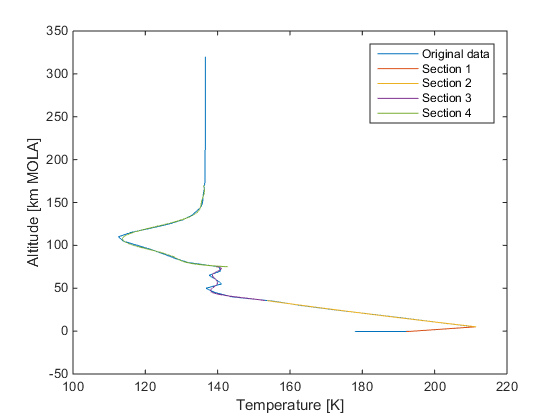
\includegraphics[width=0.7\textwidth]{figures/software/completePolyFitTempSplit5.png}
\caption{All section fits for the launch site temperature data curve}
\label{fig:completePolyFitTempSplit5}
\end{figure}



\noindent
The density fit was slightly more difficult because the curves are all very similar and thus result in a higher accuracy requirement for the fit. At first glance it looks like a natural logarithmic function, unfortunately an ordinary exponential did not fit the curve. This is why a more extensive exponential fit was required. The natural logarithm of the data has been plotted in \Cref{fig:lnPlotDataDen}.

\begin{figure}[H]
\centering
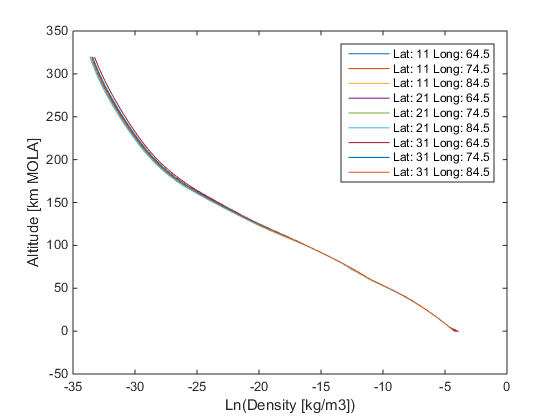
\includegraphics[width=0.7\textwidth]{figures/software/lnPlotDataDen.png}
\caption{Natural logarithmic plot of the density data}
\label{fig:lnPlotDataDen}
\end{figure}

\noindent
With the data represented in the logarithmic domain, again a polynomial function can be fitted. The total fit then satisfies \Cref{eq:expPoly}.

\begin{equation} \label{eq:expPoly}
y=\exp\left(p_{0}+p_{1}x+\dots+p_{n-1}x^{n-1}+p_{n}x^{n}\right)
\end{equation}



% A logarithmic fit (such as an exponential atmosphere) resulted in a lower overall accuracy than the polynomial fits. In this case the curve was split into three sections, because the differences between the curves were bigger in the lower atmosphere. These sections are illustrated in \Cref{fig:densityDataSplit3}.
%
% \begin{figure}[H]
%\centering
%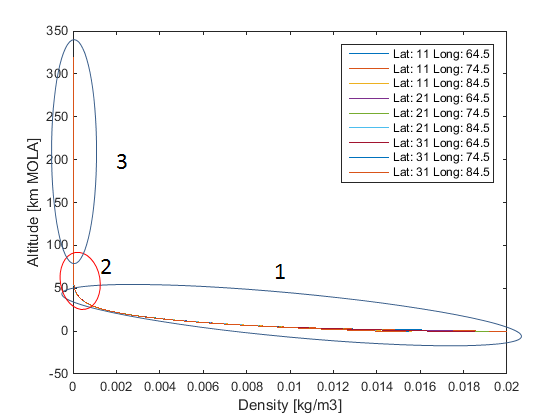
\includegraphics[width=1.0\textwidth]{figures/software/densityDataSplit3.png}
%\caption{Different density curve sections}
%\label{fig:densityDataSplit3}
%\end{figure} 

\noindent
The same polynomial requirements as for the temperature curve were enforced for the density curve as well. However, because the polynomial is used in an exponential, some extra requirements are needed to assure the accuracy of the fit. One requirement is that the maximum difference between the final exponential fit and the normal launch site density curve is smaller than the maximum difference between all the data curves. Also, in this case the standard deviation of the difference between the exponential fit and the normal launch site curve had to be within the range of standard deviations of the difference between the different data curves. This meant that even though an 8$^{\text{th}}$-order polynomial fit could be achieved for the natural logarithmic data with the required accuracy, when converted to the exponential fit, the last two requirements were not met. Earlier it was mentioned that an order higher than 8 was not desirable. However, in this case, a single exponential fit could be achieved using a 10$^\text{th}$-order polynomial. This fit meant that the density curve did not have to be split up at all, which makes the integration slightly easier. Therefore, it was decided that a 10$^\text{th}$-order polynomial was acceptable in this case. The results of the fit are presented in \Cref{tab:fitDeviationsDen,tab:fitParametersDen} and the polynomial and exponential fit curves are shown in \Cref{fig:completeExpPolyFitDen,fig:completeExpFitDen} respectively.

%
% This results in the density polynomial fit data and the polynomial parameters as presented in \Cref{tab:fitDeviationsDen,tab:fitParametersDen} respectively. 

%\textbf{\textcolor{red}{UPDATE THE NEXT TWO TABLE VALUES TO THE VALUES FOR DENSITY!!!}}

%\begin{table}[H]
%\begin{center}
%\caption{Density curve fit data (10$^{th}$ order polynomial)}
%\label{tab:fitDeviationsDen}
%\begin{tabular}{|p{3cm}|p{3cm}|p{3cm}|p{3cm}|p{3cm}|p{3cm}|p{3cm}|}
%\hline 
%\textbf{Maximum polynomial standard deviation [kg/m$^{3}$]} & \textbf{Maximum natural logarithmic curves difference [kg/m$^{3}$]} & \textbf{Maximum polynomial difference with natural logarithmic launch site curve [kg/m$^{3}$]} & \textbf{Maximum curves difference [kg/m$^{3}$]} & \textbf{Maximum difference with launch site curve [kg/m$^{3}$]} & \textbf{Maximum standard deviation curves difference [kg/m$^{3}$]} & \textbf{Standard deviation exponential fit difference [kg/m$^{3}$]} \\ \hline 
%0.0501 & 0.460 & 0.160   & 3.910$\cdot$10$^{-3}$ &  2.826$\cdot$10$^{-3}$ & 2.106$\cdot$10$^{-4}$ & 1.167$\cdot$10$^{-4}$ \\ \hline
%
%\end{tabular}
%\end{center}
%\end{table}

\begin{table}[H]
\begin{center}
\caption{Density curve fit data (10$^\text{th}$-order polynomial) with respect to the launch site curve (Latitude and longitude of the launch site)}
\label{tab:fitDeviationsDen}
{\renewcommand{\arraystretch}{1.2} % used to increase vertical spacing
\begin{tabular}{|l|l|}
\hline
\textbf{Parameter} & \textbf{Value} \\ \hline \hline 
Maximum polynomial standard deviation [ln(kg/m$^{3}$)] & 0.0501 \\ \hline

  Maximum polynomial difference [ln(kg/m$^{3}$)] & 0.160 \\ \hline
  
Maximum natural logarithmic data curves difference [ln(kg/m$^{3}$)] & 0.460 \\ \hline
  
Maximum exponential difference with launch site curve [kg/m$^{3}$] & 2.826$\cdot$10$^{-3}$ \\ \hline
    
Maximum data curves difference [kg/m$^{3}$] & 3.910$\cdot$10$^{-3}$ \\ \hline
    
Standard deviation exponential fit difference [kg/m$^{3}$] & 1.167$\cdot$10$^{-4}$ \\ \hline 
      
Maximum standard deviation data curves difference [kg/m$^{3}$] & 2.106$\cdot$10$^{-4}$ \\ \hline
\end{tabular}}
\end{center}
\end{table}



\begin{table}[H]
\begin{center}
\caption{Density curve fit parameters (rounded to 3 decimal points)}
\label{tab:fitParametersDen}
{\renewcommand{\arraystretch}{1.2} % used to increase vertical spacing
\begin{tabular}{|l|l|l|l|l|l|}
\hline 
 $\mathbf{p_{0}}$ & $\mathbf{p_{1}}$ & $\mathbf{p_{2}}$ & $\mathbf{p_{3}}$ & $\mathbf{p_{4}}$ & $\mathbf{p_{5}}$  \\ \hline
 -4.172 & -0.0962 & 1.414 $\cdot$10$^{-3}$ & -9.604 $\cdot$10$^{-5}$ & 2.273 $\cdot$10$^{-6}$ & -2.884 $\cdot$10$^{-8}$  \\ \hline 
\end{tabular}
}
\end{center}
\end{table} 
 
 
 \begin{table}[H]
\begin{center}
{\renewcommand{\arraystretch}{1.2} % used to increase vertical spacing
\begin{tabular}{|l|l|l|l|l|}
 \hline
  $\mathbf{p_{6}}$ & $\mathbf{p_{7}}$ & $\mathbf{p_{8}}$ & $\mathbf{p_{9}}$ & $\mathbf{p_{10}}$  \\ \hline 
2.146 $\cdot$10$^{-10}$ & -9.620 $\cdot$10$^{-13}$ & 2.559 $\cdot$10$^{-15}$  & -3.724 $\cdot$10$^{-18}$ & 2.287 $\cdot$10$^{-21}$  \\ \hline 
\end{tabular}
}
\end{center}
\end{table}

%The complete polynomial fit for the launch site curve for the density is shown in \Cref{fig:completePolyFitDen}.


\begin{figure}[H]
\centering
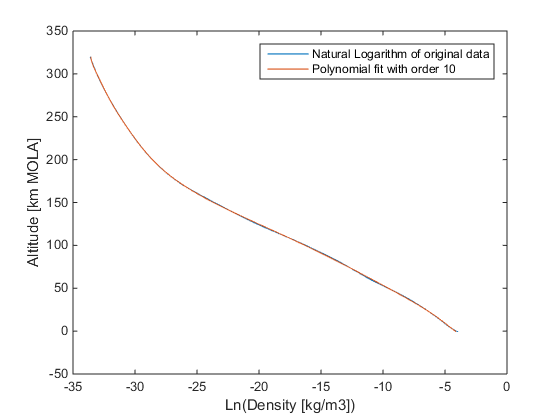
\includegraphics[width=0.7\textwidth]{figures/software/completeExpPolyFitDen.png}
\caption{Polynomial fit for the launch site density data curve.}
\label{fig:completeExpPolyFitDen}
\end{figure}

\begin{figure}[H]
\centering
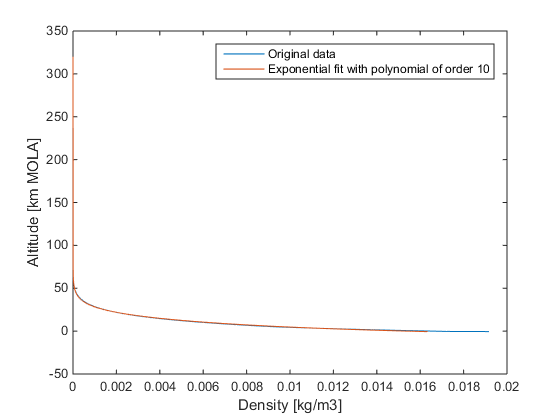
\includegraphics[width=0.7\textwidth]{figures/software/completeExpFitDen.png}
\caption{Exponential fit for the launch site density data curve.}
\label{fig:completeExpFitDen}
\end{figure}


%\begin{figure}[H]
%\centering
%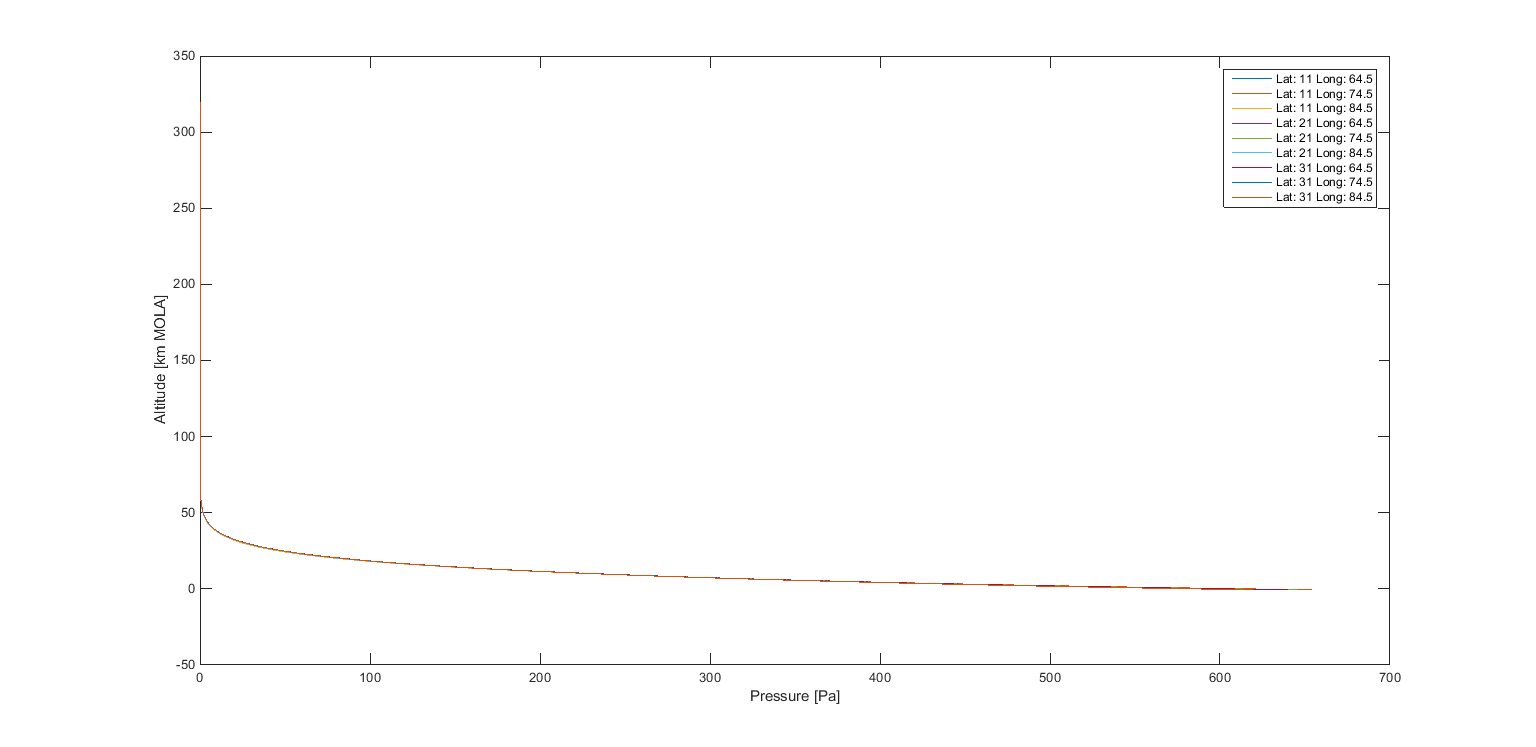
\includegraphics[width=1.0\textwidth]{figures/software/pressureData.png}
%\caption{Pressure data generated with Mars-\ac{GRAM} 2005 showing 9 different latitude and longitude combinations}
%\label{fig:pressureData}
%\end{figure}

\pagebreak

\subsection{Drag Coefficient Function Fit}
\label{subsec:dragCoefFuncFit}
Similar to the temperature and density curves, the relation between Mach number and drag coefficient, as depicted in \Cref{fig:dragcoeff_whitehead2004mars}, had to be modelled as a function as well. Again, it cannot be fitted using one single function, but instead had to be modelled by different functions. \\

\noindent
Fortunately, this curve is already an approximation and thus consists of linear elements only. It can be split up into six different sections where the first and last section are constant ($C_{D}$ is 0.2 and 0.3 respectively). Using a similar polynomial fit as before, but now for 1 order only, a linear fit could be made for each of the remaining four sections. The corresponding parameters are shown in \Cref{tab:dragCoeffPara} and the curve fit is shown in \Cref{fig:dragCoeffFit}.


\begin{table}[H]
\begin{center}
\caption{Drag coefficient curve fit parameters (rounded to 3 decimal points).}
\label{tab:dragCoeffPara}
\begin{tabular}{|l|l||l|l|}
\hline 
\textbf{Section}  & \textbf{Mach range}& $\mathbf{p_{0}}$ & $\mathbf{p_{1}}$ \\ \hline 
1 & 0 to 1  & 0.2 & 0.0 \\ \hline
2  & 0.5 to 1   & -2.483 $\cdot$10$^{-16}$ & 0.400 \\ \hline
3  & 1 to 1.3   & -0.167 & 0.567 \\ \hline
4  &  1.3 to 2.5  & 0.754 & -0.142 \\ \hline
5  &  2.5 to 4  & 0.567 & -0.0667 \\ \hline
6 & $>$4  & 0.3 & 0.0 \\ \hline
\end{tabular}
\end{center}
\end{table}



\begin{figure}[H]
\centering
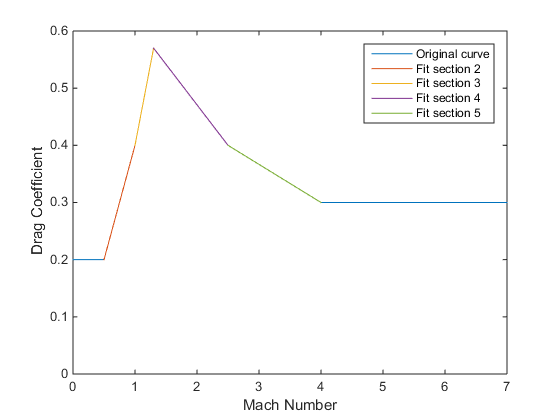
\includegraphics[width=0.7\textwidth]{figures/software/dragCoeffFit.png}
\caption{All section fits for the drag coefficient - Mach curve.}
\label{fig:dragCoeffFit}
\end{figure}

\pagebreak

\section{Circularisation}
\label{sec:modelCircularisation}
After the integration has been completed (defined by reaching either the desired altitude, mission duration or horizontal flight conditions), a circularisation burn will take place to estimate the required propellant mass to arrive in the desired orbit. This will include the $\Delta V$ required to change the flight-path angle, change the inclination and adjust the orbital velocity. A simplified diagram of such a procedure is presented in \Cref{fig:deltaVcircularOrbitMars_wakker2010}. The equations used to perform this instantaneous burn are based on the equations presented by \cite{wakker2010}.

\nomenclature[Ga2]{$\Delta V$}{Change in velocity \nomunit{m/s}}
\nomenclature[Rb0]{$V_{x}$}{Velocity in x-direction \nomunit{m/s}}
\nomenclature[Rb0]{$V_{y}$}{Velocity in y-direction \nomunit{m/s}}
\nomenclature[Rb0]{$V_{z}$}{Velocity in z-direction \nomunit{m/s}}


\begin{figure}[H]
\centering
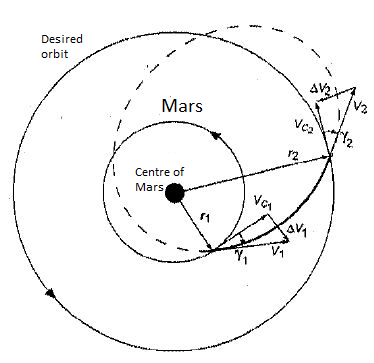
\includegraphics[width=0.3\textwidth]{figures/circularisation/deltaVcircularOrbitMars_wakker2010.png}
\caption{Circularisation into the desired orbit \citep{wakker2010}.}
\label{fig:deltaVcircularOrbitMars_wakker2010}
\end{figure}

\noindent
The first step is to convert the final cartesian state obtained at the end of the integration to Kepler elements. This conversion is a standard conversion that can be found in \cite{wakker2010} and requires the standard gravitational parameter of Mars ($\mu_{M}$), which is taken to be 4.2828314 km$^{3}$/s$^{2}$. Then using the vis-viva equation presented in \Cref{eq:visViva} the current orbital velocity of the launch trajectory can be computed. Here the subscript $co$ stands for "current orbit" and $a$ is the semi-major axis of the launch trajectory.

\begin{equation} \label{eq:visViva}
V_{co} = \sqrt{\mu_{M}\left(\dfrac{2}{r_{co}}-\dfrac{1}{a_{co}}\right)}
\end{equation}

\nomenclature[Ra0]{$a$}{Semi-major axis \nomunit{m}}

\noindent
Then the required orbital velocity is a simplified representation of the vis-viva equation because it is assumed that the required orbit is always circular, see \Cref{eq:simpVisViva}. Here $do$ stands for "desired orbit".

\begin{equation} \label{eq:simpVisViva}
V_{do}=\sqrt{\dfrac{\mu_{M}}{r_{do}}}
\end{equation} 

\noindent
Because a change in flight-path angle might be required, the current flight-path angle has to be included into the change in velocity as well. For this, the semi-latus rectum ($p$) of the current orbit has to be computed first and then the cosine of the flight-path angle can be computed as shown by \Cref{eq:cosFPA}.


\begin{equation}\label{eq:cosFPA}
\begin{split}
p_{co}&=a_{co}\left(1-e_{co}^{2}\right)\\
\cos \gamma_{co}&=\dfrac{\left(\dfrac{p_{co}}{r_{co}}\right)}{\left(\sqrt{2\left(\dfrac{p_{co}}{r_{co}}\right)-\left(1-e^{2}\right)}\right)}\\
\end{split}
\end{equation}

\noindent
The required $\Delta V$ needed to reach the desired orbit can now be computed using \Cref{eq:requiredDeltaV}.

\begin{equation} \label{eq:requiredDeltaV}
\Delta V = \sqrt{V_{do}^{2}+V_{co}^{2}-2V_{do}V_{co}\left[\cos \gamma_{co}+\cos\left(i_{do}-i_{co}\right)\right]}
\end{equation}

\nomenclature[Ra2]{$i$}{Inclination \nomunit{rad}}

\noindent
Finally, the required propellant mass can be computed using Tsiolkovsky's equation as shown by \Cref{eq:propellantMass}.

\begin{equation} \label{eq:propellantMass}
m_{prop} = m_{MAV}\left(1-e^{\dfrac{-\Delta V}{I_{sp}g_{0}}}\right)
\end{equation}

\nomenclature[Ra4]{$m_{prop}$}{Propellant mass \nomunit{kg}}
%
%m_{prop} = m_{MAV}-\dfrac{m_{MAV}}{e^{\dfrac{\Delta V}{I_{sp}g_{0}}}}

%
%\textbf{\textcolor{red}{This section still has to be added!!}}				% For thesis


%\chapter{Optimisation} %Last updated 04-03-2016
\label{ch:optimisation}		% For thesis

\chapter{Standard integration methods}
% 16-11-2016 created


\label{ch:standardIntegrationMethods}
Propagation refers to the process of modelling/predicting the manner in which an object (for instance) will progress (in time) from a starting point, usually given an initial condition. Such an initial condition could be a constant force or another kind of perturbation. In orbital computations, numerical integration is often used to model this behaviour, because of the irregularities in the dynamic environment (many perturbations) and the absence of analytical solutions. The solution then provides an estimate of the trajectory and the state of the \ac{s/c}\citep{hofsteenge2013}. There are several different types of numerical integrators that all try to predict the \ac{s/c} behaviour in different ways. These types are described in \Cref{sec:differentIntegratorTypes}. In \Cref{sec:chosenMethodForComparison} the method is chosen that will be used in this research to compare the performance of the \ac{TSI} method with. \\
Numerical integration methods do have one major drawback compared to analytic methods, and that is the accuracy of the produced result. Numerical methods come close to the actual result but usually do not reach it. Therefore, there will always be a certain error associated with the answer. One of the most important errors is called the local (and total) truncation error, which is caused by the numerical inaccuracy of the method itself, and are usually the largest errors. A second error can be introduced by the round-off properties of the used computer, which then also depends on the number of evaluations required for each of the integration methods (more evaluations means more round-off errors). These round-off errors are due to the fact that computers can only accurately represent a number up until a certain number of decimal figures. According to \cite{milani1987} there are also specific errors that arise when integrating space-related problems. Instability errors can occur if the simulated system is chaotic or if the step-size is too large.\\
Another, non-method specific and not necessarily integration related, error source is the mistakes made in the physical model representing the problem in the simulation. Such errors can occur when forces and disturbances are not (properly) taken into account in the assumptions made to create the physical model.\\
Fortunately, many of the standard integration methods already contain functions that approximate these errors and then include those approximations to come up with a better solution, or try to minimize these errors by using multiple approximations. The focus of this chapter will thus be on the different integration methods and not the different methods of determining the different errors.

\section{Different integrator types}
\label{sec:differentIntegratorTypes}
A number of different numerical integration methods exist, however in this section they will be split based on how they work. In this case they have been split into single-step (\Cref{subsec:singleStep}) and multi-step methods (\Cref{subsec:multiStep}) based on \cite{noomen2013int}. The methods can also be split based on the used step-size; either a fixed step-size that does not change during the integration, or a variable step-size that changes per step (or sometimes even during the step). Finally, the methods can also be categorised by either being explicit or implicit. An explicit method uses the information provided at the start of the integration (the current state $\mathbf{x}_{i}$ and sometimes previous states) to determine the next state $\mathbf{x}_{i+1}$. Whereas an implicit method uses the same information to determine $\mathbf{x}_{i+1}$, but once this first solution is obtained, it uses this next state as an approximation of the solution and feeds it back into the method in order to determine a more accurate solution. This requires iteration. \\
The numerical approximation of the next state can be written as the current state plus the change during one time-step. This change is defined as the step-size $h$ times the increment function 
$\mathbf{\Phi}$ as shown by \Cref{eq:integration}, which changes depending on the method used. Here, $\mathbf{\eta}$ represents the total numerical approximation. 

\nomenclature[Ra5]{$\mathbf{x}_{i}$}{Current data point\nomunit{-}}
\nomenclature[Ra6]{$\mathbf{x}_{i+1}$}{Next data point\nomunit{-}}
\nomenclature[R4]{$h$}{(Current) step-size\nomunit{s}}
\nomenclature[G8]{$\Phi$}{Increment function\nomunit{-}}
\nomenclature[G3]{$\eta$}{Numerical approximation\nomunit{-}}


\begin{equation} \label{eq:integration}
\mathbf{x}(t_{0}+h)\approx\mathbf{x}_{0}+h\bm{\Phi}=\mathbf{\eta}(t_{0}+h)
\end{equation}

\nomenclature[Ra1]{$t_{0}$}{Initial time\nomunit{s}} 



\subsection{Single-step}
\label{subsec:singleStep}
Single-step methods solely use the information at the current point to determine the approximation of the next state. This means tht the information of the previous points is neglected and usually not saved \citep{noomen2013int}. Examples of the most simple explicit, fixed step-size, single-step methods are Euler, Mid-point and \ac{RK4} \citep{hofsteenge2013}. Euler uses the information at the current state to directly compute the estimate of the next state. Mid-point already incorporates an extra estimation where it first computes a point at half the step-size and then uses that information to approximate the next state, and \ac{RK4} takes 4 points into account and takes the weighted average of those to come up with a solution (the starting point, two mid-points and a final point). Many methods exists that are based on these simple methods, for instance the Mid-point method based high-order extrapolation (a.k.a. DIFEX2) (explicit) method \citep{deuflhard1994}.\\
Many more methods however are based on the \ac{RK4} principle such as Runge-Kutta-Nystr\"{o}m (RKN, with variations such as RKN7(6)9) (implicit) \citep{montenbruck1992,dormand1987}, \ac{RKN12} (implicit) \citep{montenbruck1992}  and \acf{RKF45} and \acf{RKF78} \citep{fehlberg1969,fehlberg1968}. These last two integrators are slightly different since they are still explicit, but use a variable step-size.


\subsection{Multi-step}
\label{subsec:multiStep}
Compared to the single-step method, the multi-step method does use the information of the previous points to estimate the next state. Usually reaching as far back as the previous three points such as the \ac{AB4} method \citep{noomen2013int}, this being the only difference between this method and the \ac{RK4} method. Extending this method creates the explicit \ac{AB6} method. An example of an implicit, fixed step-size, multi-step method is the Adams-Moulton method. It uses a polynomial to interpolate the function values in order to approximate the next state \citep{noomen2013int}. Explicit and implicit methods can also be combined to create so-called Predictor-Corrector methods. Here an initial guess is created by the explicit method, which is then fed into the implicit part in order to correct and improve the estimate. Examples of Predictor-Corrector methods are \ac{ABM4} and \ac{ABM12} \citep{noomen2013int,montenbruck1992}. \\
All previously mentioned multi-step methods use a fixed step-size. Variable step-size methods also exist, such as \ac{SG} (explicit) \citep{berry2004,meijaard1991} and \ac{SC14} (Predictor-Corrector) \citep{berry2004,ramos2005}.


\section{Chosen method for comparison}
\label{sec:chosenMethodForComparison}
In order to choose the method that will be used to compare the performance of \ac{TSI} to, it was important to understand which methods were readily available. If a method is already validated and available for use a lot of time can be saved. Therefore, an inquiry of available methods is made in \Cref{subsec:tudatMethods}. Another important criteria is that the performance of \ac{TSI} should be able to be compared to previous study cases. The easiest way of doing that is to see what methods other researchers used to compare \ac{TSI} to (see \Cref{subsec:methodsUsedInPreviousResearch}. Using the information from \Cref{subsec:tudatMethods,subsec:methodsUsedInPreviousResearch} a decision could be made on the final comparison method as is described in \Cref{subsec:chosenMethod}.

\subsection{Tudat methods}
\label{subsec:tudatMethods}
One of the software tools used in this thesis is \ac{Tudat} (see \Cref{subsec:tudat} for more information). It is a computational toolbox that already comes with a number of useful functions. It also contains a number of pre-programmed validated numerical integrators. A list of the available integration methods is provided in \Cref{tab:tudatIntegrators}.


\begin{table}[!ht]
\begin{center}
\caption{Available \ac{Tudat} integrators \citep{dirkx2016tudat}}
\label{tab:tudatIntegrators}
\begin{tabular}{|l|p{4cm}|p{8cm}|l|}
\hline 
\textbf{Method} & \textbf{Kind of method}		& \textbf{File} & \textbf{Ready for use} \\ \hline \hline
\ac{RK4} 	& explicit, fixed step-size, single-step & rungeKutta4Integrator.h & Yes  \\ \hline
\ac{RKF45} 	& explicit,  variable step-size, single-step & numericalIntegrator.h \& rungeKuttaVariableStepSizeIntegrator.h
\& rungeKuttaCoefficients.h/.cpp &  Yes \\ \hline
\acs{RKF56} 	& explicit, variable step-size, single-step & numericalIntegrator.h \& rungeKuttaVariableStepSizeIntegrator.h
\& rungeKuttaCoefficients.h/.cpp & No  \\ \hline
\ac{RKF78} &	explicit, variable step-size, single-step & numericalIntegrator.h \& rungeKuttaVariableStepSizeIntegrator.h
\& rungeKuttaCoefficients.h/.cpp &  Yes \\ \hline
\acs{DOPRIN87} 	& explicit, variable step-size, single-step & numericalIntegrator.h \& rungeKuttaVariableStepSizeIntegrator.h
\& rungeKuttaCoefficients.h/.cpp & Yes  \\ \hline
 	
 		
% 	&	&  &   \\ \hline
\end{tabular}
\end{center}
\end{table}

Most of these methods are very similar except \ac{RK4} which is a fixed step-size method, and \ac{DOPRIN87} which is actually a Runge-Kutta method similar to \ac{RKF} with an accuracy order 8(7) using the formulations as described by \cite{prince1981high} according to \cite{weeks2007comparison}. At the time of the research, the \ac{RKF56} method that was preprogrammed into \ac{Tudat} was unfortunately not available for use.

\subsection{Methods used in previous research}
\label{subsec:methodsUsedInPreviousResearch}
Out of the research done on integration methods for space missions, the most relevant is the research that was done on \ac{TSI}. The research performed by \cite{scott2008high} focused on orbital trajectories and used RKF8(9) and the researched performed by \cite{bergsma2016application} focussed on re-entry cases and used \ac{RKF56}. Unfortunately, RKF8(9) was not available through \ac{Tudat} and \ac{RKF56} was out of commission at the time of this thesis research. However, it is good to notice that both researchers used higher order RKF methods, which encourages the use of similar methods for this research and fortunately similar methods are available.

\subsection{Chosen method}
\label{subsec:chosenMethod}
Considering the available methods and the methods used in previous \ac{TSI} research it was determined that the \ac{RKF} methods and \ac{DOPRIN87} would be tested in the early phases of the verification process. In this case \ac{RK4} would serve as a back-up. During the verification of the standard integrator it was found that \ac{RKF78} showed the best performance when dealing with these ascent problems, which is why it was chosen as the integration method to which \ac{TSI} was later compared.


\section{Workings of \ac{RKF}}
\label{sec:rkf}
The principle behind \ac{RKF} is perhaps best explained by first looking at a simpler Runge-Kutta method such as \ac{RK4}. \cite{noomen2013int} provides a simple explanation of the workings of \ac{RK4} that have been adapted here. In this case, use is made of the general formulation for the numerical approximation as was shown in \Cref{eq:integration}. The increment function for \ac{RK4} is then presented by \Cref{eq:rk4_increment}. In this case four points are used to approximate the next state as visualised in \Cref{fig:rk4_noomen2013int}. 

\begin{equation} \label{eq:rk4_increment}
\Phi_{RK4}=\dfrac{1}{6}\left(k_{1}+2k_{2}+2k_{3}+k_{4}\right)
\end{equation}


\begin{figure}[!ht]
\centering
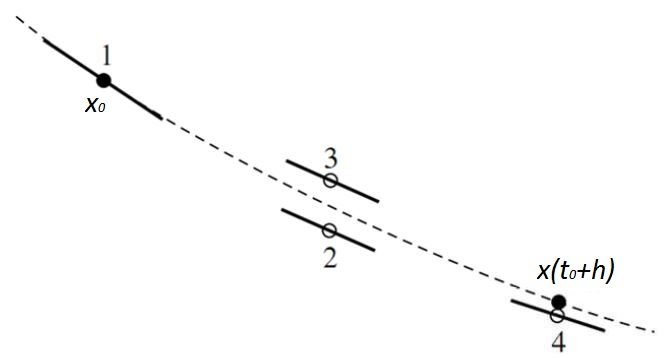
\includegraphics[width=0.3\textwidth]{figures/integrators/rk4_noomen2013int.jpg}
\caption{Principle of \ac{RK4} for a single parameter \cite{noomen2013int}.}
\label{fig:rk4_noomen2013int}
\end{figure}

Runge-Kutta works with the time-derivatives at those points. The derivative at the first point is called $k_{1}$, at the second point $k_{2}$ etcetera. These time derivatives are used both in the increment function but also in the process of determining the derivative of the next intermediate point as shown by \Cref{eq:k}.

\begin{equation} \label{eq:k}
\begin{split}
k_{1}&=f'\left(t_{0},\mathbf{x}_{0}\right)\\
k_{2}&=f'\left(t_{0}+h/2,\mathbf{x}_{0}+hk_{1}/2\right)\\
k_{3}&=f'\left(t_{0}+h/2,\mathbf{x}_{0}+hk_{2}/2\right)\\
k_{4}&=f'\left(t_{0}+h,\mathbf{x}_{0}+hk_{3}\right)\\
\end{split}
\end{equation}

\Cref{eq:rk4_increment,eq:k} can also be generalized as presented by \Cref{eq:generalRK}. In this case $b_{i}$ represents the different weights for each of the points with the corresponding step-size weights $c_{i}$, $n$ is the order and $a_{i,j}$ are the coefficients of the previous time-derivatives.

\begin{equation} \label{eq:generalRK}
\begin{split}
\Phi_{RK} &= \displaystyle \sum^{n}_{i=1}b_{i}k_{i} \\
\text{with}\quad k_{i} &= f'\left(t+c_{n}h,y+h\displaystyle \sum^{n-1}_{j=1}a_{i,j}k_{j} \right) \\
\end{split}
\end{equation}


This general formulation can now also be used to compute the higher order Runge-Kutta approximations given that $a_{i,j}$, $b_{i}$ and $c_{i}$ are provided. These sets of numbers can be found in various literature, and different people have come up with different sets. Fehlberg was one of these people. In order to get a more accurate solution he decided to use two different methods. In the case of this research, \ac{RKF78} was used, which means that a 7$^{th}$ order and 8$^{th}$ order solution can be computed using \Cref{eq:generalRK}. The 7$^{th}$ order solution is then used as the method solution and the difference between the 8$^{th}$ and the 7$^{th}$ order solution results in an error estimate which can be used to determine the next step-size. This step-size is thus computed such as to minimize this error estimate. This means that the only difference between \ac{RKF78} and \ac{RKF45} (for instance) is the coefficient set (a, b and c's). 









                  % For thesis


\chapter{Taylor series integration} %Last updated 18-05-2016
\label{ch:tsi}

\section{General theory}
\label{sec:genTsiTheory}

\subsection{Workings of \ac{TSI}}
\label{subsec:workTsi}

\subsection{Step-size}
\label{subsec:stepSizeTsi}

\section{Associated equations}
\label{sec:assEq}
In order for \ac{TSI} to be implemented, the state derivatives have to be modelled as a set of continuous functions which are a function of the state only. This can be done in different ways. In this case, three cases were tested: two Cartesian cases and one spherical case. For the Cartesian cases, the initial conditions first have to be transformed into Cartesian coordinates. The Cartesian equations themselves require reference frame transformations, which can be written in two different ways. Both cases are described in \Cref{subsec:careq}. The reason for testing the spherical case is that the initial conditions are provided in spherical coordinates and the intermediate computations can be easily interpreted and checked for errors. However, the equations are highly sensitive to singularities. The spherical equations are described in \Cref{subsec:sphereq} and already include reference frame transformations. 

\subsection{Cartesian equations}
\label{subsec:careq}
The Cartesian state is described in \Cref{eq:state}, where $m_{MAV}$ is the mass of the \ac{MAV} and the subscript $I$ refers to the inertial frame.

\begin{align} \label{eq:state}
\mathbf{r}&=\begin{pmatrix}
x_{I}\\
y_{I}\\
z_{I}\\
\end{pmatrix}
&
\mathbf{V}&=\begin{pmatrix}
V_{x_{I}} \\
V_{y_{I}} \\
V_{z_{I}}\\
\end{pmatrix}
&
m_{MAV}&
\end{align}

The corresponding state derivatives are then described by \Cref{eq:state_derivatives}.

\begin{align} \label{eq:state_derivatives}
\begin{split} 
\dot{x}_{I}&=V_{x_{I}}\\
\dot{y}_{I}&=V_{y_{I}}\\
\dot{z}_{I}&=V_{z_{I}}
\end{split} 
&
\begin{split}
\ddot{x}_{I}&=\dot{V}_{x_{I}}=a_{x_{I}}\\
\ddot{y}_{I}&=\dot{V}_{y_{I}}=a_{y_{I}}\\
\ddot{z}_{I}&=\dot{V}_{z_{I}}=a_{z_{I}}
\end{split}
&
\dot{m}_{MAV}=-\dfrac{T}{g_{0}I_{sp}}
\end{align}

From this point on, the subscript $I$ is omitted, because the state and the state derivatives are always presented in the inertial frame. If variables have to be presented in any other reference frame the corresponding subscripts will be provided and explained. The accelerations in the x-, y- and z-direction have three contributing components: gravitational acceleration, drag and thrust. The gravitational acceleration can be directly expressed in the inertial frame, however the drag is presented in the body frame and the thrust is expressed in the propulsion frame. Therefore, both the drag and thrust contributions have to be transformed to the inertial frame using transformation matrices. This then results in the expression for the acceleration vector as shown by \Cref{eq:acc}. The subscript $G$ shows that the parameter is a function of the ground velocity.

\begin{multline} \label{eq:acc}
\begin{pmatrix}
a_{x}\\
a_{y}\\
a_{z}\\
\end{pmatrix}
=
\begin{pmatrix}
-\mu_{M}\dfrac{x}{r^{3}}\\
-\mu_{M}\dfrac{y}{r^{3}}\\
-\mu_{M}\dfrac{z}{r^{3}}\\
\end{pmatrix}+
\Bigg|_{\mathbf{I}}\mathbb{T}_{\mathbf{z}}\left(-\Omega_{M}t_{O}+\omega_{P}\right)\Bigg|_{\mathbf{R}}\mathbb{T}_{\mathbf{z}}\left(-\tau\right)\mathbb{T}_{\mathbf{y}}\left(\dfrac{\pi}{2}+\delta\right)\Bigg|_{\mathbf{V}}\mathbb{T}_{\mathbf{z}}\left(-\chi_{G}\right)\mathbb{T}_{\mathbf{y}}\left(-\gamma_{G}\right)\Bigg|_{\mathbf{B}}\left[
\begin{pmatrix}
-\dfrac{D}{m_{MAV}}\\
0\\
0\\
\end{pmatrix}
+  \right. \dots \\
\dotsc
 \left.
\Bigg|_{\mathbf{B}}\mathbb{T}_{\mathbf{z}}\left(-\psi_{T}\right)\mathbb{T}_{\mathbf{y}}\left(-\epsilon_{T}\right)\Bigg|_{\mathbf{P}}
\begin{pmatrix}
\dfrac{T}{m_{MAV}}\\
0\\
0\\
\end{pmatrix}
\right]
\end{multline}

It can be seen that this set of equations is a function of the current position and many other parameters. These parameters will all have to be written as a function of the current state. This can be done by writing them into auxiliary equations, forming extra variables that then also require the auxiliary derivatives. This works for certain parameters, such as the gravity, because these equations are already expressed in the inertial frame. However, the transformation angles are defined in different reference frames, which means that finding the proper auxiliary derivatives can be tricky sometimes. Therefore it was decided to directly write these parameters as auxiliary functions. Each of the auxiliary functions performs one simple algebraic operation and the collection of these auxiliary functions then form the complete set of recurrence relations using the recurrence relations for the simple algebraic operations. This is all described in \Cref{subsec:recRelAuxFunc}. 

For the auxiliary equations, a similar notation will be used as shown by \cite{scott2008high}. Here the equations are denoted by $x_{number}$ and the corresponding derivatives $x'_{number}$. This notation will also be used for the current state and the corresponding state derivatives. This way, \Cref{eq:state} can be written as \Cref{eq:stateX} and the corresponding derivatives can be written as presented by \Cref{eq:state_derivativesX}.

\begin{align} \label{eq:stateX}
\begin{split} 
x_{1}&=x\\
x_{2}&=y\\
x_{3}&=z
\end{split} 
&
\begin{split}
x_{4}&=\dot{x}=V_{x}\\
x_{5}&=\dot{y}=V_{y}\\
x_{6}&=\dot{z}=V_{z}
\end{split}
&
x_{7}=m_{MAV}
\end{align}


\begin{align} \label{eq:state_derivativesX}
\begin{split} 
x'_{1}&=x_{4}\\
x'_{2}&=x_{5}\\
x'_{3}&=x_{6}
\end{split} 
&
\begin{split}
x'_{4}&=\dot{V}_{x}=a_{x}=a_{g,x}+a_{D,x}+a_{T,x}\\
x'_{5}&=\dot{V}_{y}=a_{y}=a_{g,y}+a_{D,y}+a_{T,y}\\
x'_{6}&=\dot{V}_{z}=a_{z}=a_{g,z}+a_{D,z}+a_{T,z}
\end{split}
&
x'_{7}=\dot{m}_{MAV}=-\dfrac{T}{g_{0}I_{sp}}
\end{align}

In this case the thrust and specific impulse are constant, which means that $x'_{7}$ is constant and any additional derivative will be zero. Also, neither one of the thrust angles is a function of the state, which means that $a_{T}$, in the body frame, is only a function of $x_{7}$ (also see \Cref{eq:acc}). However, both $a_{g}$ and $a_{D}$ are a function of the position and velocity, where $a_{D}$ is also a function of the \ac{MAV} mass. Only $a_{g}$ is rewritten using auxiliary equations as mentioned before. This is shown in \Cref{subsubsec:tsiGravity}.


%For the numbering of all the auxiliary equations goes that the order comes from the manner in which they were all written out on paper. This means that sometimes higher number parameters could contain much lower number parameters without the intermediate parameters defined yet. However, these will all be defined eventually.


\subsubsection{Gravitational acceleration}
 \label{subsubsec:tsiGravity} 
 For the gravitational acceleration two auxiliary equations were required since $r=\sqrt{x^{2}+y^{2}+z^{2}}$. The resulting expressions for the gravitational acceleration are shown in \Cref{eq:gravAcc} with the corresponding auxiliary equations and the derivatives defined in \Cref{eq:gravAux}.
 
 \begin{equation} \label{eq:gravAcc}
\begin{split}
a_{g,x} &= -\mu_{M}\dfrac{x_{1}}{r^{3}} = \dfrac{x_{1}}{\left(x_{1}^{2}+x_{2}^{2}+x_{3}^{2} \right)^{3/2}}=-\mu_{M}\dfrac{x_{1}}{x_{9}}\\
a_{g,y} &= -\mu_{M}\dfrac{x_{2}}{r^{3}} = \dfrac{x_{2}}{\left(x_{1}^{2}+x_{2}^{2}+x_{3}^{2} \right)^{3/2}}=-\mu_{M}\dfrac{x_{2}}{x_{9}}\\
a_{g,z} &= -\mu_{M}\dfrac{x_{3}}{r^{3}} = \dfrac{x_{3}}{\left(x_{1}^{2}+x_{2}^{2}+x_{3}^{2} \right)^{3/2}}=-\mu_{M}\dfrac{x_{3}}{x_{9}}
\end{split}
\end{equation}

\begin{align} \label{eq:gravAux}
\begin{split} 
x_{8}&=x_{1}^{2}+x_{2}^{2}+x_{3}^{2}\\
x_{9}&=x_{8}^{3/2}
\end{split} 
&
\begin{split}
x'_{8}&=2x_{1}x_{4}+2x_{2}x_{5}+2x_{3}x_{6}\\
x'_{9}&=\dfrac{3}{2}\dfrac{x_{9}x_{8}'}{x_{8}}
\end{split}
\end{align}
 
 
 
\subsubsection{Transformation angles}
\label{subsubsec:tsiTransAngl}
The angles required for the transformation to go from the body frame to the reference frame all have to be written as a function of the state variables. The required angles are $\lambda$, $\delta$, $\chi_{G}$ and $\gamma_{G}$. Here $\lambda = \tau + \Omega_{M}t_{O}-\omega_{P}$. This means that instead of first transforming to the rotating frame completely and then transforming to the inertial frame, an inertial longitude angle $\lambda$ can be defined to directly transform to the inertial frame. The first two angles are the longitude and latitude and are spherical coordinates. Thus the relations for these angles can be found using the transformation from the Cartesian to the spherical system. However, the angles themselves are not required directly, because they are only used in transformation matrices. These matrices are comprised of the sines and cosines of these angles, which means that a direct relation between the state variables and the sines and cosines of the position angles can be used. These relations can be derived from \Cref{fig:sphertocart_noomen2013basic} and are described in \Cref{eq:transAngl}


 \begin{figure}[!ht]
\centering
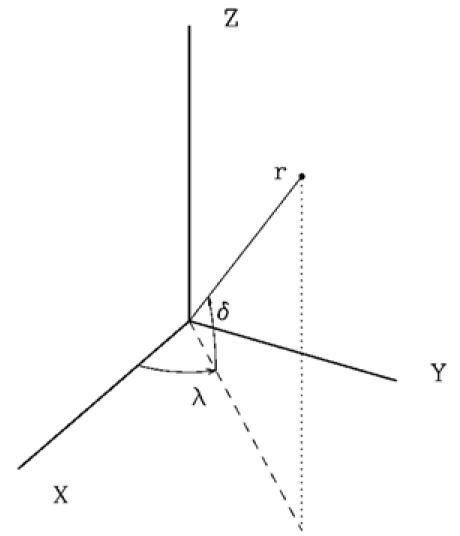
\includegraphics[width=0.7\textwidth]{figures/reference_frames/sphertocart_noomen2013basic.jpg}
\caption{Spherical position variables in an inertial Cartesian frame \citep{noomen2013basic}.}
\label{fig:sphertocart_noomen2013basic}
\end{figure}

\begin{align} \label{eq:transAngl}
\begin{split}
r = \sqrt{x^{2}+y^{2}+z^{2}}\\
\end{split}
&
\begin{split}
\sin \lambda &= \dfrac{y}{\sqrt{x^{2}+y^{2}}}\\
\cos \lambda &= \dfrac{x}{\sqrt{x^{2}+y^{2}}}\\
\end{split}
&
\begin{split}
\sin \delta &= \dfrac{z}{r}\\
\cos \delta &= \dfrac{\sqrt{x^{2}+y^{2}}}{r}
\end{split} 
\end{align} 

The corresponding auxiliary functions can then be described by \Cref{eq:auxFtransAngl} using the definitions provided in \Cref{eq:stateX,eq:state_derivativesX}.

\begin{align} \label{eq:AuxFtransAngl}
\begin{split}
w_{4,1} &= x_{1}^{2}+x_{2}^{2} \\
w_{4,2} &= w_{4,1}+x_{3}^{2} \\
w_{4,3} &= r = \sqrt{w_{4,2}} \\
w_{4,4} &= \sqrt{w_{4,1}} \\
\end{split}
&
\begin{split}
w_{4,5} &= s\lambda = \dfrac{x_{2}}{w_{4,4}}\\
w_{4,6} &= c\lambda = \dfrac{x_{1}}{w_{4,4}} \\
\end{split}
&
\begin{split}
w_{4,7} &= s\delta = \dfrac{x_{3}}{w_{4,3}} \\
w_{4,8} &= c\delta = \dfrac{w_{4,4}}{w_{4,3}}\\
\end{split} 
\end{align} 


The latitude and longitude could be described using the position vector in the inertial frame, however the transformation from the body frame to the vertical frame is a function of the ground (underscore 'G') velocity in the rotational frame. Since the position and velocity in the inertial frame are known (current state), the ground velocity ($V_{G}$) can be written as a function of the inertial velocity ($V_{I}$). For this, the velocity components have to be transformed from the inertial frame to the vertical frame (which is the inverse of the first three transformations described in \Cref{eq:acc}). This transformation is shown in \Cref{eq:VItoVV} and was described in \cite{mooij1994motion}. Here, $c$ stands for cosine and $s$ stands for sine. This transformation also includes the rotational effect on the velocity due to the rotation of Mars.
 
 \begin{equation} \label{eq:VItoVV}
\mathbf{V_{V}} =  
 \begin{pmatrix}
V_{x_{V}}\\
V_{y_{V}}\\
V_{z_{V}}\\
\end{pmatrix}
=
\left[
\begin{matrix}
-c\lambda s\delta & -s\lambda s\delta & c\delta\\
-s\lambda & c\lambda & 0\\
-c\lambda c\delta & -s\lambda c\delta & -s\delta\\
\end{matrix}
\right]
\left\lbrace
\begin{pmatrix}
V_{x}\\
V_{y}\\
V_{z}\\
\end{pmatrix}
-
\begin{pmatrix}
0 \\
0 \\
\Omega_{M} \\
\end{pmatrix}
\times
\begin{pmatrix}
x \\
y \\
z \\
\end{pmatrix}
\right\rbrace
 \end{equation}
 
The ground velocity can now be computed as the norm of the vertical velocity vector as shown by \Cref{eq:VG}. The transformation matrices disappear because the norm of a transformation matrix is simply 1, which means that $V_{G}=V_{V}=V_{R}$.

\begin{equation} \label{eq:VG}
V_{G} = \| \mathbf{V_{V}} \| = 
\left\Vert
\begin{pmatrix}
V_{x}\\
V_{y}\\
V_{z}\\
\end{pmatrix}
-
\begin{pmatrix}
0 \\
0 \\
\Omega_{M} \\
\end{pmatrix}
\times
\begin{pmatrix}
x \\
y \\
z \\
\end{pmatrix}
\right\Vert 
\end{equation}

\Cref{eq:VG} can be rewritten as \Cref{eq:xfifteen}.

\begin{equation}\label{eq:xfifteen}
V_{G} = \sqrt{\left(V_{x}+\Omega_{M}y\right)^{2}+\left(V_{y}-\Omega_{M}x\right)^{2}+V_{z}^{2}} 
\end{equation}

The corresponding auxiliary functions are provided in \Cref{eq:velocityAuxF}.

\begin{align} \label{eq:velocityAuxF}
\begin{split}
w_{4,9} &= V_{x}+\Omega_{M}y \\
w_{4,10} &= V_{y}-\Omega_{M}x \\
\end{split}
&
\begin{split}
w_{4,11} &= w_{4,9}^{2}+w_{4,10}^{2}+x_{6}^{2} \\
w_{4,12} &= V_{G}=\sqrt{w_{4,11}} \\
\end{split} 
\end{align} 

%\sqrt{V_{I}^{2}+\Omega_{M}^{2}\left(x^{2}+y^{2}\right)+2\Omega_{M}\left(V_{x}y-V_{y}x\right)} \quad \text{where} \quad V_{I}=\sqrt{V_{x}^{2}+V_{y}^{2}+V_{z}^{2}} \\
 
The spherical velocity angles can now be derifed from \Cref{fig:vertical_spherical_mooij1994motion} as described by \Cref{eq:velAngl}. These were also provided by \cite{mooij1994motion}. 

 \begin{figure}[!ht]
\centering
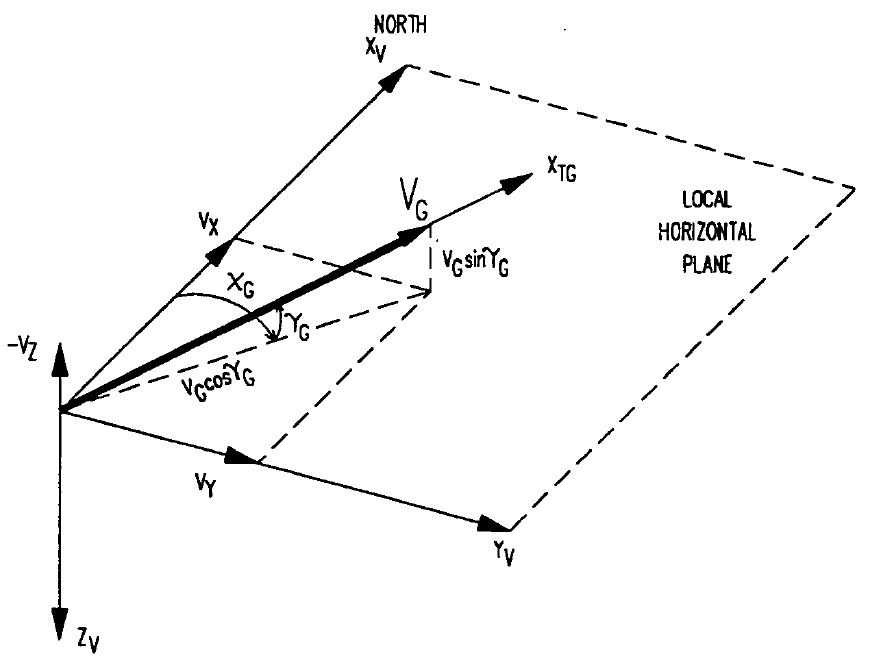
\includegraphics[width=0.7\textwidth]{figures/reference_frames/vertical_spherical_mooij1994motion.jpg}
\caption{Spherical velocity variables in a vertical Cartesian frame \citep{mooij1994motion}.}
\label{fig:vertical_spherical_mooij1994motion}
\end{figure}



\begin{align} \label{eq:velAngl}
\begin{split}
\sin \chi_{G} &= \dfrac{V_{y_{V}}}{\sqrt{V_{x_{V}}^{2}+V_{y_{V}}^{2}}} \\
\cos \chi_{G} &= \dfrac{V_{x_{V}}}{\sqrt{V_{x_{V}}^{2}+V_{y_{V}}^{2}}} \\
\end{split}
&
\begin{split}
\sin \gamma_{G} &= \dfrac{-V_{z_{V}}}{V_{G}}\\
\cos \gamma_{G} &= \dfrac{\sqrt{V_{x_{V}}^{2}+V_{y_{V}}^{2}}}{V_{G}}\\
\end{split} 
\end{align} 


Here, $V_{x_{V}}$, $V_{y_{V}}$ and $V_{z_{V}}$ are the velocities in the vertical frame. Expressions for these variables can be obtained by rewriting \Cref{eq:VItoVV}. This then results in \Cref{eq:VV}.


\begin{equation} \label{eq:VV}
\begin{split}
V_{x_{V}} & = -\left(V_{x}+\Omega_{M}y\right) s \delta c\lambda - \left(V_{y}-\Omega_{M}x\right) s\delta s\lambda+V_{z}c\delta \\
V_{y_{V}} & = \left(V_{y}-\Omega_{M}x\right) c\lambda - \left(V_{x}+\Omega_{M} y \right) s\lambda \\
V_{z_{V}} & = -\left(V_{x}+\Omega_{M}y\right)-\left(V_{y}-\Omega_{M}x\right) c\delta s\lambda - V_{z} s\delta \\
\end{split}
\end{equation}

The combined auxiliary functions for \Cref{eq:velAngl,eq:VV} are described in \Cref{eq:velocityAuxF}.

\begin{align} \label{eq:VV}
\begin{split}
w_{4,13} &= -c\lambda s\delta  = -w_{4,6}w_{4,7} \\
w_{4,14} &= -s\delta s\lambda = -w_{4,7}w_{4,5} \\
w_{4,15} &= -c\delta c\lambda = -w_{4,8}w_{4,6} \\
w_{4,16} &= -c\delta s\lambda = w_{4,8}w_{4,5} \\
\end{split}
&
\begin{split}
w_{4,17} &= V_{x_{V}} = x_{6}w_{4,8}+w_{4,9}w_{4,13}+w_{4,10}w_{4,14} \\
w_{4,18} &= V_{y_{V}} = w_{4,10}w_{4,6}-w_{4,9}w_{4,5} \\
w_{4,19} &= V_{z_{V}} = w_{4,9}w_{4,15}-x_{6}w_{4,7}+w_{4,10}w_{4,16} \\
w_{4,20} &= V_{x_{V}}^{2}+V_{y_{V}}^{2} = w_{4,17}^{2}+w_{4,18}^{2} \\
w_{4,21} &= \sqrt{w_{4,20}} \\
\end{split}
&
\begin{split}
w_{4,22} &= s\chi_{G} = \dfrac{w_{4,18}}{w_{4,21}} \\
w_{4,23} &= c\chi_{G} = \dfrac{w_{4,17}}{w_{4,21}} \\
w_{4,24} &= s\gamma_{G} = -\dfrac{w_{4,19}}{w_{4,12}} \\
w_{4,25} &= c\gamma_{G} = \dfrac{w_{4,21}}{w_{4,12}} \\
\end{split}
\end{align}



 \subsubsection{Drag acceleration}
 \label{subsubsec:tsiDrag}
The drag acceleration is determined in the body frame by dividing the drag force ($D$) by the mass of the \ac{MAV} ($x_{7}$). The drag force itself is a function of the position and velocity. The equations associated with the drag function are described in \Cref{eq:dragAux} except for the $C_{D}$ equations. The polynomial coefficients for the density equation are provided in \Cref{tab:fitParametersDen} and are represented in \Cref{eq:dragAux} by $P_{\rho}$.

 \begin{equation} \label{eq:dragAux}
\begin{split}
h &= r-R_{MOLA} \\
D &= \frac{1}{2}\rho V_{G}^{2}SC_{D}\\
\rho &= e^{P_{\rho 10}h^{10}+P_{\rho 9}h^{9}+P_{\rho 8}h^{8}+P_{\rho 7}h^{7}+P_{\rho 6}h^{6}+P_{\rho 5}h^{5}+P_{\rho 4}h^{4}+P_{\rho 3}h^{3}+P_{\rho 2}h^{2}+P_{\rho 1}h+P_{\rho 0}} \\
\end{split}
\end{equation}

The numbering for the drag auxiliary functions start with 27 because it was added later on and because it used to be an auxiliary equation. The auxiliary functions for the density can then be described by \Cref{eq:dragAuxF}.

\begin{align} \label{eq:dragAuxF}
\begin{split}
w_{27,1} &= h = w_{4,3} - R_{MOLA} \\
w_{27,2} &= w_{27,1}^{2}\\
w_{27,3} &= w_{27,1}^{3}\\
w_{27,4} &= w_{27,1}^{4}\\
w_{27,5} &= w_{27,1}^{5}\\
w_{27,6} &= w_{27,1}^{6}\\
\end{split}
&
\begin{split}
w_{27,7} &= w_{27,1}^{7}\\
w_{27,8} &= w_{27,1}^{8}\\
w_{27,9} &= w_{27,1}^{9}\\
w_{27,10} &= w_{27,1}^{10}\\
w_{27,11} &= P_{\rho 10}w_{27,10}+P_{\rho 9}w_{27,9}+\dotsc +P_{\rho 1}w_{27,1}+P_{\rho 0}\\
w_{27,12} &= \rho = e^{w_{27,11}} \\
\end{split}
\end{align}

Since the drag coefficient is a function of Mach number as by \Cref{fig:dragcoeff_whitehead2004mars} and is not a continuous function, it has to be split into 6 different sections. Each section has a separate $C_{D}-M$ relation. Before these relations can be described, three additional expressions are required which are described in \Cref{eq:cdAux}.

 \begin{equation} \label{eq:cdAux}
\begin{split}
M &= \dfrac{V_{G}}{a} \\
a &= \sqrt{\gamma_{a}R_{a}^{*}T_{a}} \quad \text{where} \quad R_{a}^{*}=\dfrac{R_{a}}{M_{a}} \\
\end{split}
\end{equation}

Where the corresponding auxiliary functions can be described by \Cref{eq:cdAuxF}.

\begin{align} \label{eq:cdAuxF}
\begin{split}
w_{27,14} &= a = \sqrt{\gamma_{a}R_{a}^{*}w_{27,13}}  \\
w_{27,15} &= M = \dfrac{w_{4,12}}{27,14} \\
\end{split}
\end{align}

The conditional relations shown in \Cref{eq:cdCond} describe the different equations that have to be used associated with the different sections of the drag coefficient plot. Here $P_{C_{D} number,section}$ are the polynomial fit coefficients as provided in \Cref{tab:dragCoeffPara}.

\begin{equation}\label{eq:cdCond}
C_{D}=\begin{cases}
0.2, & \text{for } 0\leq M < 0.5\\
P_{C_{D} 1,2}M+P_{C_{D} 0,2}, &  \text{for } 0.5\leq M < 1 \\
P_{C_{D} 1,3}M+P_{C_{D} 0,3}, &  \text{for } 1\leq M < 1.3 \\
P_{C_{D} 1,4}M+P_{C_{D} 0,4}, &  \text{for } 1.3\leq M < 2.5 \\
P_{C_{D} 1,5}M+P_{C_{D} 0,5}, &  \text{for } 2.5\leq M < 4 \\
0.3, &  \text{for } M \geq 4 
\end{cases}\\
\end{equation}

In this case, the auxiliary functions for $C_{D} \left( = w_{27,16}\right)$ is any of the conditional relations depending on $M \left( = w_{27,15}\right)$.

This only leaves the temperature $T_{a} \left(= w_{27,13}\right)$ , which is a function of the altitude $h \left(= w_{27,1} \right) $ in km,\ac{MOLA}. But as described in \Cref{subsec:atmofuncfit}, this parameter is split into different sections as well. The equations per section for the temperature is provided in \Cref{eq:tempCondAux}. Here $P_{T number,section}$ are the polynomial fit coefficients as provided in \Cref{tab:fitParameters}.

\begin{equation}\label{eq:tempCondAux}
T_{a}=\begin{cases}
P_{T 1,1}h+P_{T 0,1}, & \text{for } -0.6 \leq h < 5.04  \\
P_{T 3,2}h^{3}+P_{T 2,2}h^{2}+P_{T 1,2}h+P_{T 0,2}, &  \text{for } 5.04 \leq h < 35.53   \\
P_{T 6,3}h^{6}+P_{T 5,3}h^{5}+P_{T 4,3}h^{4}+P_{T 3,3}h^{3}+ \dotsc \\
\qquad\ \ \dotsc +P_{T 2,3}h^{2}+P_{T 1,3}h+P_{T 0,3}, &  \text{for } 35.53 \leq h < 75.07   \\
P_{T 8,4}h^{8}+P_{T 7,4}h^{7}+P_{T 6,4}h^{6}+P_{T 5,4}h^{5}+ \dotsc \\
\qquad\ \ \dotsc+P_{T 4,4}h^{4}+P_{T 3,4}h^{3}+P_{T 2,4}h^{2}+P_{T 1,4}h+P_{T 0,4}, &  \text{for } 75.07 \leq h < 170.05   \\
136.5, &  \text{for }  h \geq 170.05   
\end{cases}
\end{equation}

For both the conditional parameters $C_{D}$ and $T_{a}$  the required section has to be determined before the evaluation of the equations.

The drag can now also be described as an auxiliary function as shown by \Cref{eq:dragAuxF}.

\begin{align} \label{eq:dragAuxF}
\begin{split}
w_{27,17} &= V_{G}^{2} =  w_{4,12}^{2} \\
w_{27,18} &= V_{G}^{2}C_{D} = w_{27,17}w_{27,16} \\
w_{27,19} &= D = \frac{1}{2} S w_{27,18}w_{27,12} \\
\end{split}
\end{align}



\subsubsection{Thrust acceleration}
\label{subsubsec:tsiDrag}
The only acceleration component still missing is the thrust acceleration. To be able to write the auxiliary functions for the thrust, \Cref{eq:acc} first has to be rewritten such that all the transformations are gathered into two transformation matrices (see \Cref{eq:accAux}). The transformation matrices are described by \Cref{eq:BPtrans,eq:IBtrans} for $\mathbb{T}_{\mathbf{BP}}$ and $\mathbb{T}_{\mathbf{IB}}$ respectively.

\begin{equation} \label{eq:accAux}
\begin{pmatrix}
x'_{4}\\
x'_{5}\\
x'_{6}\\
\end{pmatrix}
=
\begin{pmatrix}
-\mu_{M}\dfrac{x_{1}}{x_{9}}\\
-\mu_{M}\dfrac{x_{2}}{x_{9}}\\
-\mu_{M}\dfrac{x_{3}}{x_{9}}\\
\end{pmatrix}+
\mathbb{T}_{\mathbf{IB}}\left[
\begin{pmatrix}
-\dfrac{w_{27,19}}{x_{7}}\\
0\\
0\\
\end{pmatrix}
+ 
\mathbb{T}_{\mathbf{BP}}
\begin{pmatrix}
\dfrac{T}{x_{7}}\\
0\\
0\\
\end{pmatrix}
\right]
\end{equation}


\begin{equation} \label{eq:BPtrans}
\mathbb{T}_{\mathbf{BP}}=
\begin{bmatrix}
c\psi_{T}c\epsilon_{T} & -s\psi_{T} & c\psi_{T}s\epsilon_{T}\\
s\psi_{T}c\epsilon_{T} & c\psi_{T} & s\psi_{T}s\epsilon_{T}\\
-s\epsilon_{T} & 0 & c\epsilon_{T}\\
\end{bmatrix}
\end{equation}

\begin{equation} \label{eq:IBtrans}
\mathbb{T}_{\mathbf{IB}}=
\left[
\begin{matrix}
c\lambda\left(-s\delta c\chi c\gamma +c\delta s\gamma \right)-s\lambda s\chi c\gamma  & c\lambda s\delta s\chi -s\lambda c\chi & c\lambda\left(-s\delta c\chi s\gamma -c\delta c\gamma \right)-s\lambda s\chi s\gamma \\
s\lambda\left(-s\delta c\chi c\gamma +c\delta s\gamma \right)+c\lambda s\chi c\gamma & s\lambda s\delta s\chi +c\lambda c\chi & s\lambda\left(-s\delta c\chi s\gamma -c\delta c\gamma \right)+c\lambda s\chi s\gamma \\
c\delta c\chi c\gamma +s\delta s\gamma &  -c\delta s\chi &  c\delta c\chi s\gamma -s\delta c\gamma \\
\end{matrix}
\right]\\
\end{equation}

 \textbf{\textcolor{red}{Rest still has to be rewritten!!}}

%\end{matrix}  \right.
%\\
%\begin{matrix}
%c\lambda s\delta s\chi -s\lambda c\chi\\
%s\lambda s\delta s\chi +c\lambda c\chi \\
% -c\delta s\chi \\
%\end{matrix}
%\\
%\left.
%\begin{matrix}
%c\lambda\left(-s\delta c\chi s\gamma -c\delta c\gamma \right)-s\lambda s\chi s\gamma\\
%s\lambda\left(-s\delta c\chi s\gamma -c\delta c\gamma \right)+c\lambda s\chi s\gamma \\
%c\delta c\chi s\gamma -s\delta c\gamma\\
%=
%\left[
%\begin{matrix}
%c\left(x_{10}+x_{11}\right)\left(-sx_{12} cx_{13} cx_{14} +cx_{12} sx_{14} \right)-s\left(x_{10}+x_{11}\right) sx_{13} cx_{14}    \\
%s\left(x_{10}+x_{11}\right)\left(-sx_{12} cx_{13} cx_{14} +cx_{12} sx_{14} \right)+c\left(x_{10}+x_{11}\right) sx_{13} cx_{14}    \\
%cx_{12} cx_{13} cx_{14} +sx_{12} sx_{14}   \\
%\end{matrix} \right.
%\\
%\begin{matrix}
%c\left(x_{10}+x_{11}\right) sx_{12} sx_{13} -s\left(x_{10}+x_{11}\right) cx_{13} \\
%s\left(x_{10}+x_{11}\right) sx_{12} sx_{13} +c\left(x_{10}+x_{11}\right) cx_{13} \\
%-cx_{12} sx_{13} \\
%\end{matrix}
%\\
%\left.
%\begin{matrix}
%c\left(x_{10}+x_{11}\right)\left(-sx_{12} cx_{13} sx_{14} -cx_{12} cx_{14} \right)-s\left(x_{10}+x_{11}\right) sx_{13} sx_{14} \\
%s\left(x_{10}+x_{11}\right)\left(-sx_{12} cx_{13} sx_{14} -cx_{12} cx_{14} \right)+c\left(x_{10}+x_{11}\right) sx_{13} sx_{14} \\
% cx_{12} cx_{13} sx_{14} -sx_{12} cx_{14} \\
%\end{matrix}
%\right]\\

Because the mass flow rate is constant, and not a function of the state, the first derivative of $u_{7}$ will be zero such that $u'_{7}=0$. This means that only the first derivative of the mass flow rate has to be used and thus $u_{7}$ does not require any recurrence relations. This is not the case for the thrust accelerations because they are a function of the state (in this case $x_{7}$) and will require recurrence relations. Using an intermediate notation for the thrust accelerations in the x-, y- and z-directions, the last part of \Cref{eq:accAux} can be rewritten to \Cref{eq:aTB} using \Cref{eq:BPtrans}.

\begin{equation} \label{eq:aTB}
\mathbb{T}_{\mathbf{BP}}
\begin{pmatrix}
\dfrac{T}{x_{7}}\\
0\\
0\\
\end{pmatrix}
=
\begin{pmatrix}
\dfrac{T}{x_{7}}c\psi_{T}c\epsilon_{T}\\
\dfrac{T}{x_{7}}s\psi_{T}c\epsilon_{T}\\
-\dfrac{T}{x_{7}}s\epsilon_{T}\\
\end{pmatrix}
=
\begin{pmatrix}
a_{T_{B},x}\\
a_{T_{B},y}\\
a_{T_{B},z}\\
\end{pmatrix}
\end{equation}


The thrust accelerations are now written in the body frame, which means that they can be combined with the drag acceleration in the body frame. This is done in \Cref{eq:DandTBody}. However, since both the thrust and drag accelerations include auxiliary equations ($x_{7}$ and $x_{27}$) the total acceleration in the body frame in the different directions have to be expressed as auxiliary functions. Each auxiliary function replaces one algebraic operation such as multiplication, division, power, exponential and trigonometric functions. Auxiliary functions will be represented by $w_{n,m}$ as per convention introduced by \cite{scott2008high}. Here $n$ stands for the associating derivative and $m$ represents the number of the auxiliary function for that particular derivative. These auxiliary functions will be used to write the different parameters into recurrence relations.

\begin{equation} \label{eq:DandTBody}
\begin{pmatrix}
-\dfrac{x_{27}}{x_{7}}\\
0\\
0\\
\end{pmatrix}
+
\begin{pmatrix}
a_{T_{B},x}\\
a_{T_{B},y}\\
a_{T_{B},z}\\
\end{pmatrix}
=
\begin{pmatrix}
a_{T_{B},x}-\dfrac{x_{27}}{x_{7}}\\
a_{T_{B},y}\\
a_{T_{B},z}\\
\end{pmatrix}
=
\begin{pmatrix}
a_{T,D_{B},x}\\
a_{T_{B},y}\\
a_{T_{B},z}\\
\end{pmatrix}
=
\begin{pmatrix}
w_{4,2}\\
w_{4,33}\\
-w_{4,34}\\
\end{pmatrix}
\end{equation}

Now transforming the drag and thrust accelerations from the body frame to the inertial frame using $\mathbb{T}_{\mathbf{IB}}$ results in \Cref{eq:DandTInertial}.


\begin{multline} \label{eq:DandTInertial}
\begin{pmatrix}
a_{T,D_{I},x}\\
a_{T_{I},y}\\
a_{T_{I},z}\\
\end{pmatrix}
=
\mathbb{T}_{\mathbf{IB}}
\begin{pmatrix}
a_{T,D_{B},x}\\
a_{T_{B},y}\\
a_{T_{B},z}\\
\end{pmatrix}=
\mathbb{T}_{\mathbf{IB}}
\begin{pmatrix}
w_{4,2}\\
w_{4,33}\\
-w_{4,34}\\
\end{pmatrix}\\
=
\left(
\begin{matrix}
w_{4,2} \left( c\left(x_{10}+x_{11}\right)\left(-sx_{12} cx_{13} cx_{14} +cx_{12} sx_{14} \right)-s\left(x_{10}+x_{11}\right) sx_{13} cx_{14} \right)  + \dots  \\
w_{4,2} \left( s\left(x_{10}+x_{11}\right)\left(-sx_{12} cx_{13} cx_{14} +cx_{12} sx_{14} \right)+c\left(x_{10}+x_{11}\right) sx_{13} cx_{14}  \right)  + \dots \\
w_{4,2} \left(cx_{12} cx_{13} cx_{14} +sx_{12} sx_{14}  \right)  - \dots \\
\end{matrix} \right.
\\
\begin{matrix}
\dotsc  w_{4,33} \left( c\left(x_{10}+x_{11}\right) sx_{12} sx_{13} -s\left(x_{10}+x_{11}\right) cx_{13}\right)  - \dots \\
\dotsc  w_{4,33} \left( s\left(x_{10}+x_{11}\right) sx_{12} sx_{13} +c\left(x_{10}+x_{11}\right) cx_{13} \right)  - \dots \\
\dotsc  w_{4,33} cx_{12} sx_{13} - \dots \\
\end{matrix}
\\
\left.
\begin{matrix}
\dotsc w_{4,34} \left( c\left(x_{10}+x_{11}\right)\left(-sx_{12} cx_{13} sx_{14} -cx_{12} cx_{14} \right)-s\left(x_{10}+x_{11}\right) sx_{13} sx_{14} \right) \\
\dotsc w_{4,34} \left(s\left(x_{10}+x_{11}\right)\left(-sx_{12} cx_{13} sx_{14} -cx_{12} cx_{14} \right)+c\left(x_{10}+x_{11}\right) sx_{13} sx_{14} \right) \\
\dotsc w_{4,34} \left( cx_{12} cx_{13} sx_{14} -sx_{12} cx_{14} \right) \\
\end{matrix}
\right)\\
\end{multline}

Now including the gravity components as well, the (lengthy) expressions for $u_{4}$, $u_{5}$ and $u_{6}$ become \Cref{eq:u4Com,eq:u5Com,eq:u6Com} respectively.

\begin{equation} \label{eq:u4Com}
\begin{split}
u_{4}= -\mu_{M}\dfrac{x_{1}}{x_{9}}&+w_{4,2} \left( c\left(x_{10}+x_{11}\right)\left(-sx_{12} cx_{13} cx_{14} +cx_{12} sx_{14} \right)-s\left(x_{10}+x_{11}\right) sx_{13} cx_{14} \right)+ \dots \\
& \dotsc  w_{4,33} \left( c\left(x_{10}+x_{11}\right) sx_{12} sx_{13} -s\left(x_{10}+x_{11}\right) cx_{13}\right)-\dots \\
& \dotsc w_{4,34} \left( c\left(x_{10}+x_{11}\right)\left(-sx_{12} cx_{13} sx_{14} -cx_{12} cx_{14} \right)-s\left(x_{10}+x_{11}\right) sx_{13} sx_{14} \right)
\end{split}
\end{equation}

\begin{equation} \label{eq:u5Com}
\begin{split}
u_{5}= -\mu_{M}\dfrac{x_{2}}{x_{9}}&+w_{4,2} \left( s\left(x_{10}+x_{11}\right)\left(-sx_{12} cx_{13} cx_{14} +cx_{12} sx_{14} \right)+c\left(x_{10}+x_{11}\right) sx_{13} cx_{14}  \right)+ \dots \\
& \dotsc w_{4,33} \left( s\left(x_{10}+x_{11}\right) sx_{12} sx_{13} +c\left(x_{10}+x_{11}\right) cx_{13} \right)- \dots \\
& \dotsc w_{4,34} \left(s\left(x_{10}+x_{11}\right)\left(-sx_{12} cx_{13} sx_{14} -cx_{12} cx_{14} \right)+c\left(x_{10}+x_{11}\right) sx_{13} sx_{14} \right)
\end{split}
\end{equation} 

\begin{equation} \label{eq:u6Com}
\begin{split}
u_{6}= -\mu_{M}\dfrac{x_{3}}{x_{9}}&+w_{4,2} \left(cx_{12} cx_{13} cx_{14} +sx_{12} sx_{14}  \right)  - w_{4,33}cx_{12} sx_{13}  -w_{4,34} \left( cx_{12} cx_{13} sx_{14} -sx_{12} cx_{14} \right)
\end{split}
\end{equation}

\subsection{Spherical equations}
\label{subsec:sphereq}


 
 \subsubsection{Drag acceleration}
 \label{subsubsec:tsiDrag}
The drag acceleration is determined in the body frame by dividing the drag force ($D$) by the mass of the \ac{MAV} ($x_{7}$). The drag force itself is a function of the position and velocity. The equations associated with the drag function are described in \Cref{eq:dragAux} and the corresponding derivatives are presented by \Cref{eq:dragDerAux} except for the $C_{D}$ equations. The polynomial coefficients for the density equation are provided in \Cref{tab:fitParametersDen} and are represented in \Cref{eq:dragAux} by $P_{\rho}$.

 \begin{equation} \label{eq:dragAux}
\begin{split}
h &= r-R_{MOLA} \\
D &= \frac{1}{2}\rho V_{G}^{2}SC_{D}\\
\rho &= e^{P_{\rho 10}h^{10}+P_{\rho 9}h^{9}+P_{\rho 8}h^{8}+P_{\rho 7}h^{7}+P_{\rho 6}h^{6}+P_{\rho 5}h^{5}+P_{\rho 4}h^{4}+P_{\rho 3}h^{3}+P_{\rho 2}h^{2}+P_{\rho 1}h+P_{\rho 0}} \\
\end{split}
\end{equation}

 \begin{equation} \label{eq:dragDerAux}
\begin{split}
x'_{27} &= \frac{1}{2}Sx_{15}\left(x_{15} \left(x_{29}x'_{28}+x_{28}x'_{29}\right)+2x_{28}x_{29}x'_{15}\right) \\
x'_{28} &= x'_{30}x_{28} \\
x'_{30} &=x'_{31} \left(10 P_{\rho 10}x_{31}^{9}+9 P_{\rho 9}x_{31}^{8}+8 P_{\rho 8}x_{31}^{7}+7 P_{\rho 7}x_{31}^{6}+6 P_{\rho 6}x_{31}^{5}+\dots \right. \\
&  \left. \dotsc +5 P_{\rho 5}x_{31}^{4}+4 P_{\rho 4}x_{31}^{3}+3 P_{\rho 3}x_{31}^{2}+2 P_{\rho 2}x_{31}+P_{\rho 1}\right) \\
x'_{31} &= x'_{16}
\end{split}
\end{equation}

Since the drag coefficient is a function of Mach number as by \Cref{fig:dragcoeff_whitehead2004mars} and is not a continuous function, it had to be split into 6 different sections. Each section has a separate $C_{D}-M$ relation. Before these relations can be described, three additional auxiliary equations/expressions are required which are described in \Cref{eq:cdAux}.

 \begin{equation} \label{eq:cdAux}
\begin{split}
x_{32} &= M = \dfrac{V}{a} = \dfrac{x_{15}}{x_{33}}\\
x_{33} &= a = \sqrt{\gamma_{a}R_{a}^{*}T_{a}} = \sqrt{\gamma_{a}R_{a}^{*}x_{34}} \quad \text{where} \quad R_{a}^{*}=\dfrac{R_{a}}{M_{a}} \\
x_{34} &= T_{a}
\end{split}
\end{equation}

The conditional relations shown in \Cref{eq:cdCond} describe the different auxiliary equations that have to be used associated with the different sections. Here $P_{C_{D} number,section}$ are the polynomial fit coefficients as provided in \Cref{tab:dragCoeffPara}.

\begin{equation}\label{eq:cdCond}
x_{29}=C_{D}=\begin{cases}
x_{29,1}=0.2, & \text{for } 0\leq x_{32} < 0.5\\
x_{29,2}=P_{C_{D} 1,2}x_{32}+P_{C_{D} 0,2}, &  \text{for } 0.5\leq x_{32} < 1 \\
x_{29,3}=P_{C_{D} 1,3}x_{32}+P_{C_{D} 0,3}, &  \text{for } 1\leq x_{32} < 1.3 \\
x_{29,4}=P_{C_{D} 1,4}x_{32}+P_{C_{D} 0,4}, &  \text{for } 1.3\leq x_{32} < 2.5 \\
x_{29,5}=P_{C_{D} 1,5}x_{32}+P_{C_{D} 0,5}, &  \text{for } 2.5\leq x_{32} < 4 \\
x_{29,6}=0.3, &  \text{for } x_{32} \geq 4 
\end{cases}\\
\end{equation}

The corresponding derivatives are presented \Cref{eq:cdCondDer}.

\begin{equation}\label{eq:cdCondDer}
x'_{29}=\begin{cases}
x'_{29,1}=0, & \text{for } 0\leq x_{32} < 0.5\\
x'_{29,2}=P_{C_{D} 1,2}x'_{32}, &  \text{for } 0.5\leq x_{32} < 1 \\
x'_{29,3}=P_{C_{D} 1,3}x'_{32}, &  \text{for } 1\leq x_{32} < 1.3 \\
x'_{29,4}=P_{C_{D} 1,4}x'_{32}, &  \text{for } 1.3\leq x_{32} < 2.5 \\
x'_{29,5}=P_{C_{D} 1,5}x'_{32}, &  \text{for } 2.5\leq x_{32} < 4 \\
x'_{29,6}=0, &  \text{for } x_{32} \geq 4 
\end{cases}\\
\end{equation}

The Mach derivative and corresponding speed of sound derivative are described in \Cref{eq:cdDerAux}.

 \begin{equation} \label{eq:cdDerAux}
\begin{split}
x'_{32} &= \dfrac{x_{33}x'_{15}-x_{15}x'_{33}}{x_{33}^{2}}\\
x'_{33} &= \dfrac{\gamma_{a}R_{a}^{*}}{2x_{33}}x'_{34} 
\end{split}
\end{equation}

This only leaves the temperature $T_{a}$, which is a function of the altitude $h$ ($x_{31}$) in km,\ac{MOLA}. But as described in \Cref{subsec:atmofuncfit}, this parameter is split into different sections as well. The auxiliary equations per section for the temperature is provided in \Cref{eq:tempCondAux}. Here $P_{T number,section}$ are the polynomial fit coefficients as provided in \Cref{tab:fitParameters}.

\begin{equation}\label{eq:tempCondAux}
x_{34}=T_{a}=\begin{cases}
x_{34,1}=P_{T 1,1}x_{31}+P_{T 0,1}, & \text{for } -0.6 \leq x_{31} < 5.04  \\
x_{34,2}=P_{T 3,2}x_{31}^{3}+P_{T 2,2}x_{31}^{2}+P_{T 1,2}x_{31}+P_{T 0,2}, &  \text{for } 5.04 \leq x_{31} < 35.53   \\
x_{34,3}=P_{T 6,3}x_{31}^{6}+P_{T 5,3}x_{31}^{5}+P_{T 4,3}x_{31}^{4}+P_{T 3,3}x_{31}^{3}+ \dots \\
\qquad\ \ \dotsc +P_{T 2,3}x_{31}^{2}+P_{T 1,3}x_{31}+P_{T 0,3}, &  \text{for } 35.53 \leq x_{31} < 75.07   \\
x_{34,4}=P_{T 8,4}x_{31}^{8}+P_{T 7,4}x_{31}^{7}+P_{T 6,4}x_{31}^{6}+P_{T 5,4}x_{31}^{5} \\
\qquad\ \ +P_{T 4,4}x_{31}^{4}+P_{T 3,4}x_{31}^{3}+P_{T 2,4}x_{31}^{2}+P_{T 1,4}x_{31}+P_{T 0,4}, &  \text{for } 75.07 \leq x_{31} < 170.05   \\
x_{34,5}=136.5, &  \text{for }  x_{31} \geq 170.05   
\end{cases}
\end{equation}

The corresponding derivatives are presented \Cref{eq:TCondDerAux}.

\begin{equation}\label{eq:TCondDerAux}
x'_{34}=\begin{cases}
x'_{34,1}=P_{T 1,1}x'_{31}, & \text{for } -0.6 \leq x_{31} < 5.04  \\
x'_{34,2}=\left(3P_{T 3,2}x_{31}^{2}+2P_{T 2,2}x_{31}+P_{T 1,2}\right)x'_{31}, &  \text{for } 5.04\leq x_{31} < 35.53   \\
x'_{34,3}=\left(6 P_{T 6,3}x_{31}^{5}+5P_{T 5,3}x_{31}^{4}+4P_{T 4,3}x_{31}^{3}+ \dots
\right. \\
\qquad\  \left. \dotsc +3P_{T 3,3}x_{31}^{2}+2P_{T 2,3}x_{31}+P_{T 1,3}\right)x'_{31}, &  \text{for } 35.53\leq x_{31} < 75.07   \\
x'_{34,4}=\left(8 P_{T 8,4}x_{31}^{7}+7P_{T 7,4}x_{31}^{6}+6P_{T 6,4}x_{31}^{5}
+5P_{T 5,4}x_{31}^{4}+ \dots \right. \\
\qquad\  \left. \dotsc +4P_{T 4,4}x_{31}^{3}+3P_{T 3,4}x_{31}^{2}+2P_{T 2,4}x_{31}+P_{T 1,4}\right)x'_{31}, &  \text{for } 75.07\leq x_{31} < 170.05   \\
x'_{34,5}=0, &  \text{for }  x_{31} \geq 170.05   
\end{cases}
\end{equation}


For both the conditional parameters $C_{D}$ ($x_{29}$) and $T_{a}$ ($x_{34}$) the required section has to be determined before the evaluation of the auxiliary equations.
 

\subsection{Recurrence relations and auxiliary functions}
\label{subsec:recRelAuxFunc}
To be able to determine the different auxiliary functions and eventually write the recurrence relations each of the derivatives presented in \Cref{subsec:auxEq} will be rewritten using \Cref{eq:un} as by \cite{scott2008high}. 

\begin{equation} \label{eq:un}
u_{n}=x'_{n}, \quad n=1,\dotsc,49
\end{equation}

These equations are then written as presented by \Cref{eq:unAuxEq1,eq:unAuxEq2}.

\begin{align} \label{eq:unAuxEq1}
\begin{split} 
u_{1}&=x_{4}\\
u_{2}&=x_{5}\\
u_{3}&=x_{6} \\
u_{4}&=\dot{V}_{x}=a_{x}=a_{g,x}+a_{D,x}+a_{T,x}\\
u_{5}&=\dot{V}_{y}=a_{y}=a_{g,y}+a_{D,y}+a_{T,y}\\
u_{6}&=\dot{V}_{z}=a_{z}=a_{g,z}+a_{D,z}+a_{T,z}\\
\end{split}
&
\begin{split}
u_{7} &=\dot{m}_{MAV}=-\dfrac{T}{g_{0}I_{sp}}\\
u_{8}&=2x_{1}x_{4}+2x_{2}x_{5}+2x_{3}x_{6}\\
u_{9}&=\dfrac{3}{2}\dfrac{x_{9}u_{8}}{x_{8}}\\
u_{10} &= \Omega_{M} \\
u_{11} &=  \dot{\tau} = \dfrac{x_{15}sx_{13}cx_{14}}{x_{16}cx_{12}}\\
\end{split}
\end{align}

\begin{align} \label{eq:unAuxEq2}
\begin{split} 
u_{12} &= \dot{\delta} = \dfrac{x_{15}cx_{13}cx_{14}}{x_{16}}\\
u_{13} &= \dot{\chi}_{G} = 2\dfrac{\Omega_{M}}{cx_{14}}\left(sx_{12}cx_{14}-cx_{12}sx_{14}cx_{13}\right)+\dfrac{x_{15}}{x_{16}}cx_{14}tx_{12}sx_{13}+\dfrac{\Omega_{M}^{2}}{x_{15}cx_{14}}x_{16}cx_{12}s_{x12}sx_{13}-\dfrac{T}{x_{15}cx_{14}x_{7}}s\psi_{T}c\epsilon_{T} \\
u_{14} &= \dot{\gamma}_{G} = 2\Omega_{M}cx_{12}sx_{13}+\dfrac{x_{15}}{x_{16}}cx_{14}+\dfrac{\Omega_{M}^{2}}{x_{15}}x_{16}cx_{12}\left(cx_{12}cx_{14}+sx_{14}sx_{12}cx_{13}\right)+\dfrac{T}{x_{15}x_{7}}s\epsilon_{T}-\dfrac{\mu_{M}}{x_{15}x_{16}^{2}}cx_{14} \\
u_{15} &= \dot{V}_{G} = \Omega_{M}^{2}x_{16}cx_{12}\left(sx_{14}cx_{12}-cx_{14}sx_{12}cx_{13}\right)+\dfrac{T}{x_{7}}c\psi_{T}c\epsilon_{T}-\dfrac{x_{27}}{x_{7}}-\dfrac{\mu_{M}}{x_{16}^{2}}sx_{14} \\
u_{16} &= \dot{r}_{G} = x_{15}sx_{14}\\
\end{split}
\end{align}


\begin{equation} \label{eq:unAuxEq3}
\begin{split}
u_{27} &=  \frac{1}{2}Sx_{15}\left(x_{15} \left(x_{29}u_{28}+x_{28}u_{29}\right)+2x_{28}x_{29}u_{15}\right) \\
u_{28} &= u_{30}x_{28} \\
u_{29} &=\begin{cases}
u_{29,1}=0, & \text{for } 0\leq x_{32} < 0.5\\
u_{29,2}=P_{C_{D} 1,2}u_{32}, &  \text{for } 0.5\leq x_{32} < 1 \\
u_{29,3}=P_{C_{D} 1,3}u_{32}, &  \text{for } 1\leq x_{32} < 1.3 \\
u_{29,4}=P_{C_{D} 1,4}u_{32}, &  \text{for } 1.3\leq x_{32} < 2.5 \\
u_{29,5}=P_{C_{D} 1,5}u_{32}, &  \text{for } 2.5\leq x_{32} < 4 \\
u_{29,6}=0, &  \text{for } x_{32} \geq 4 
\end{cases}\\
u_{30} &=u_{31} \left(10 P_{\rho 10}x_{31}^{9}+9 P_{\rho 9}x_{31}^{8}+8 P_{\rho 8}x_{31}^{7}+7 P_{\rho 7}x_{31}^{6}+6 P_{\rho 6}x_{31}^{5}+5 P_{\rho 5}x_{31}^{4}\dots \right. \\
& \left. \dotsc +4 P_{\rho 4}x_{31}^{3}+3 P_{\rho 3}x_{31}^{2}+2 P_{\rho 2}x_{31}+P_{\rho 1}\right) \\
u_{31} &= u_{16}\\
u_{32} &= \dfrac{x_{33}u_{15}-x_{15}u_{33}}{x_{33}^{2}}\\
u_{33} &= \dfrac{\gamma_{a}R_{a}^{*}}{2x_{33}}u_{34} \\
u_{34}&=\begin{cases}
u_{34,1}=P_{T 1,1}u_{31}, & \text{for } -0.6 \leq x_{31} < 5.04  \\
u_{34,2}=\left(3P_{T 3,2}x_{31}^{2}+2P_{T 2,2}x_{31}+P_{T 1,2}\right)u_{31}, &  \text{for } 5.04\leq x_{31} < 35.53   \\
u_{34,3}=\left(6 P_{T 6,3}x_{31}^{5}+5P_{T 5,3}x_{31}^{4}+4P_{T 4,3}x_{31}^{3}+\dots \right. \\
\qquad \ \  \left. \dotsc +3P_{T 3,3}x_{31}^{2}+2P_{T 2,3}x_{31}+P_{T 1,3}\right)u_{31}, &  \text{for } 35.53\leq x_{31} < 75.07   \\
u_{34,4}=\left(8 P_{T 8,4}x_{31}^{7}+7P_{T 7,4}x_{31}^{6}+6P_{T 6,4}x_{31}^{5}+5P_{T 5,4}x_{31}^{4} + \dots \right. \\
\qquad \ \  \left. \dotsc +4P_{T 4,4}x_{31}^{3}+3P_{T 3,4}x_{31}^{2}+2P_{T 2,4}x_{31}+P_{T 1,4}\right)u_{31}, &  \text{for } 75.07\leq x_{31} < 170.05   \\
u_{34,5}=0, &  \text{for }  x_{31} \geq 170.05   
\end{cases}
\end{split}
\end{equation}





 
%
%\subsubsection{Auxiliary functions}
%\label{subsubsec:auxFunc}

To be able to compute the initial values of the auxiliary equations ($x_{n}$) and their derivatives($u_{n}$) they all have to be computed in a certain order. Unfortunately, because of the manner in which these were defined, the order is not simply the order in which they were numbered. Therefore \Cref{tab:calcOrderAuxEq} shows the required order in which they have to be computed. In order to avoid confusion the auxiliary equations are computed first and then the derivatives.

\begin{table}[!ht]
\begin{center}
\caption{Order of auxiliary equations and derivatives computations}
\label{tab:calcOrderAuxEq}
\begin{tabular}{|l|l||l|l||l|l||l|l|}
\hline 
\multicolumn{4}{c}{\textbf{Auxiliary equations}} & \multicolumn{4}{c}{\textbf{Auxiliary derivatives}} \\ \hline \hline
\textbf{Order} & $\mathbf{x_{n}}$ &\textbf{Order} & $\mathbf{x_{n}}$ & \textbf{Order} & $\mathbf{u_{n}}$ & \textbf{Order} & $\mathbf{u_{n}}$ \\ \hline 
0 & $ x_{1}, x_{2}, x_{3}, x_{4}, x_{5}, x_{6}, x_{7} $ & 5 & $ x_{32} $ & 9 & $ u_{1}, u_{2}, u_{3}, u_{4}, u_{5}, u_{6}, u_{7}, u_{8},  $ &  12 & $ u_{28}, u_{33} $ \\ \cline{1-4} \cline{7-8}
1 & $ x_{8}, x_{9}, x_{10}, x_{15}, x_{16} $ &  6 & $ x_{29} $ &  & $ u_{10}, u_{11}, u_{12}, u_{13}, u_{14}, u_{15}, u_{16} $ &  13 & $ u_{32} $ \\ \hline
2 & $ x_{11}, x_{12}, x_{31} $ & 7 & $ x_{27} $ & 10 & $ u_{9}, u_{31} $ &  14 & $ u_{29} $ \\ \hline
3 & $ x_{13}, x_{14}, x_{30}, x_{34} $ &  8 & $ w_{4,2}, w_{4,33}, $ & 11 & $ u_{30}, u_{34} $ &  15 & $ u_{27} $ \\ \cline{1-2} \cline{5-8}
4 & $ x_{28}, x_{33} $ &  & $ w_{4,34} $ & 12 & $ u_{28}, u_{33} $ & & $  $ \\ \hline

\end{tabular}
\end{center}
\end{table}



The first auxiliary functions were already introduced in \Cref{eq:DandTBody}, however, many more are required to be able to write the recurrence relations. All auxiliary functions are presented in \Cref{tab:auxFunc}, where the convention was used as introduced earlier. In this case, the entire equation was already written out when the auxiliary function numbers were assigned, which is why these can simply be computed in the order as presented. Except for $w_{4,2}$, because this is the only subtraction and requires $w_{4,32}$, $w_{4,25}$, because $w_{4,37}$ has to be multiplied with the constant thrust, and $w_{4,33}$ and $w_{4,34}$. This is due to the number assignment and the later addition of the thrust auxiliary functions. 


\begin{longtable}{|p{1.5cm}|l|p{2cm}|}
\caption{Auxiliary functions as a function of the auxiliary equations and derivatives.}
\label{tab:auxFunc}
\endfirsthead
\endhead
\hline
\textbf{Auxiliary function} & \textbf{Equation} & \textbf{Category}  \\ \hline \hline
\hline 
$w_{4,0}=$  & $ \dfrac{x_{27}}{x_{7}} $ & Division \\ \hline
$w_{4,1}=$  & $ \dfrac{x_{1}}{x_{9}} $ & Division \\ \hline
$w_{4,2}=$  & $ w_{4,32}-w_{4,0} $ & Subtraction \\ \hline
$w_{4,3}=$  & $ c\left(x_{10}+x_{11}\right) $ & Cosine  \\ \hline
$w_{4,4}=$  & $ sx_{12} $ & Sine \\ \hline
$w_{4,5}=$  & $ cx_{13} $ & Cosine  \\ \hline
$w_{4,6}=$  & $ cx_{12} $ & Cosine \\ \hline
$w_{4,7}=$  & $ sx_{14} $ & Sine \\ \hline
$w_{4,8}=$  & $ s\left(x_{10}+x_{11}\right) $ & Sine \\ \hline
$w_{4,9}=$ & $ sx_{13} $ & Sine \\ \hline
$w_{4,10}=$ & $ w_{4,4}w_{4,5} $ & Multiplication  \\ \hline
$w_{4,11}=$ & $ w_{4,6}w_{4,7} $ &  Multiplication \\ \hline
$w_{4,12}=$ & $ w_{4,9}w_{4,38} $ & Multiplication  \\ \hline
$w_{4,13}=$ & $ w_{4,4}w_{4,9} $ &  Multiplication \\ \hline
$w_{4,14}=$ & $ w_{4,8}w_{4,5} $ & Multiplication \\ \hline
$w_{4,15}=$ & $ w_{4,6}w_{4,38} $ &  Multiplication \\ \hline
$w_{4,16}=$ & $ w_{4,9}w_{4,7} $ & Multiplication  \\ \hline
$w_{4,17}=$ & $ w_{4,10}w_{4,38} $ & Multiplication \\ \hline
$w_{4,18}=$ & $ w_{4,8}w_{4,12} $ & Multiplication  \\ \hline
$w_{4,19}=$ & $ w_{4,3}w_{4,13} $ &  Multiplication \\ \hline
$w_{4,20}=$ & $ w_{4,10}w_{4,7} $ &  Multiplication \\ \hline
$w_{4,21}=$ & $ w_{4,8}w_{4,16} $ &  Multiplication \\ \hline
$w_{4,22}=$ & $ w_{4,3}\left(w_{4,11}-w_{4,17}\right) $ & Multiplication  \\ \hline
$w_{4,23}=$ & $ w_{4,3}\left(-w_{4,20}-w_{4,15}\right) $ &  Multiplication \\ \hline
$w_{4,24}=$ & $ w_{4,2}\left(w_{4,22}-w_{4,18}\right) $ &  Multiplication \\ \hline
$w_{4,25}=$  & $ T w_{4,37} $ & Constant  \\ 
& & Multiplication \\ \hline
$w_{4,26}=$  & $ c\psi_{T}  $ & Cosine  \\ \hline
$w_{4,27}=$  & $ c\epsilon_{T}  $ & Cosine  \\ \hline
$w_{4,28}=$  & $ s\psi_{T}  $ & Sine  \\ \hline
$w_{4,29}=$  & $ s\epsilon_{T}  $ & Sine  \\ \hline
$w_{4,30}=$ & $ w_{4,26}w_{4,27} $ &  Multiplication \\ \hline
$w_{4,31}=$ & $ w_{4,28}w_{4,27} $ &  Multiplication \\ \hline
$w_{4,32}=$ & $ w_{4,25}w_{4,30} $ &  Multiplication \\ \hline
$w_{4,33}=$ & $ w_{4,25}w_{4,31} $ &  Multiplication \\ \hline
$w_{4,34}=$ & $ w_{4,25}w_{4,29} $ &  Multiplication \\ \hline
$w_{4,35}=$ & $ w_{4,33}\left(w_{4,19}-w_{4,14}\right) $ &  Multiplication \\ \hline
$w_{4,36}=$ & $ w_{4,34}\left(w_{4,23}-w_{4,21}\right) $ &  Multiplication \\ \hline
$w_{4,37}=$  & $ \dfrac{1}{x_{7}} $ & Power \\ \hline
$w_{4,38}=$  & $ cx_{14}  $ & Cosine  \\ \hline
$w_{5,1}=$ & $ \dfrac{x_{2}}{x_{9}} $ & Division  \\ \hline
$w_{5,2}=$ & $ w_{4,8}\left(w_{4,11}-w_{4,17}\right) $ & Multiplication  \\ \hline
$w_{5,3}=$ & $ w_{4,3}w_{4,12} $ & Multiplication \\ \hline
$w_{5,4}=$ & $ w_{4,8}w_{4,13} $ & Multiplication  \\ \hline
$w_{5,5}=$ & $ w_{4,3}w_{4,5} $ &  Multiplication  \\ \hline
$w_{5,6}=$ & $ w_{4,8}\left(-w_{4,20}-w_{4,11}\right) $ &  Multiplication  \\ \hline
$w_{5,7}=$ & $ w_{4,3}w_{4,16} $ & Multiplication \\ \hline
$w_{5,8}=$ & $ w_{4,2}\left(w_{5,2}+w_{5,3}\right) $ & Multiplication \\ \hline
$w_{5,9}=$ & $ w_{4,33}\left(w_{5,4}+w_{5,5}\right) $ & Multiplication \\ \hline
$w_{5,10}=$ & $ w_{4,34}\left(w_{5,6}+w_{5,7}\right) $ & Multiplication \\ \hline
$w_{6,0}=$ & $ w_{4,4}w_{4,7} $ & Multiplication \\ \hline
$w_{6,1}=$ & $ \dfrac{x_{3}}{x_{9}} $ & Division \\ \hline
$w_{6,2}=$ & $ w_{4,5}w_{4,15} $ & Multiplication \\ \hline
$w_{6,3}=$ & $ w_{4,6}w_{4,9} $ & Multiplication \\ \hline
$w_{6,4}=$ & $ w_{4,5}w_{4,11} $ & Multiplication \\ \hline
$w_{6,5}=$ & $ w_{4,4}w_{4,38} $ & Multiplication \\ \hline
$w_{6,6}=$ & $ w_{4,2}\left(w_{6,2}+w_{6,0}\right) $ & Multiplication \\ \hline
$w_{6,7}=$ & $ w_{4,33}w_{6,3} $ & Multiplication \\ \hline
$w_{6,8}=$ & $ w_{4,34}\left(w_{6,4}-w_{6,5}\right) $ & Multiplication \\ \hline
$w_{8,1}=$ & $ x_{1}x_{4} $ & Multiplication \\ \hline
$w_{8,2}=$ & $ x_{2}x_{5} $ & Multiplication \\ \hline
$w_{8,3}=$ & $ x_{3}x_{6} $ & Multiplication \\ \hline
$w_{9}=$ & $ \dfrac{x_{9}u_{8}}{x_{8}} $ & Multiplication and Division \\ \hline
$w_{11,1}=$ & $ \dfrac{x_{15}}{x_{16}} $ & Division\\ \hline
$w_{11,2}=$ & $ \dfrac{w_{4,12}}{w_{4,6}} $ & Division \\ \hline
$w_{11,3}=$ & $ w_{11,1}w_{11,2} $ & Multiplication \\ \hline
$w_{12,1}=$ & $ w_{4,5}w_{4,38} $ & Multiplication \\ \hline
$w_{12,2}=$ & $ w_{11,1}w_{12,1} $ & Multiplication \\ \hline
$w_{13,0}=$ & $ \dfrac{x_{16}}{x_{15}} $ & Division \\ \hline
$w_{13,1}=$ & $ w_{4,5}w_{4,11} $ & Multiplication \\ \hline
$w_{13,2}=$ & $ \dfrac{w_{4,4}}{w_{4,6}} $ & Division \\ \hline
$w_{13,3}=$ & $ \dfrac{w_{4,4}}{w_{4,38}} $ & Division \\ \hline
$w_{13,4}=$ & $ x_{15}w_{4,38} $ & Multiplication \\ \hline
$w_{13,5}=$ & $ w_{13,0}w_{4,12} $ & Multiplication \\ \hline
$w_{13,6}=$ & $ w_{11,1}w_{13,3} $ & Multiplication \\ \hline
$w_{13,7}=$ & $ \dfrac{w_{6,5}-w_{13,1}}{w_{4,38}} $ & Division \\ \hline
$w_{13,8}=$ & $ w_{13,5}w_{13,2} $ & Multiplication \\ \hline
$w_{13,9}=$ & $ w_{13,6}w_{6,3} $ & Multiplication \\ \hline
$w_{13,10}=$ & $ \dfrac{w_{4,33}}{w_{13,4}} $ & Division \\ \hline
$w_{14,1}=$ & $ x_{16}^{2} $ & Power \\ \hline
$w_{14,2}=$ & $ w_{11,1}w_{4,38} $ & Multiplication \\ \hline
$w_{14,3}=$ & $ w_{13,0}w_{4,6} $ & Multiplication \\ \hline
$w_{14,4}=$ & $ w_{6,0}w_{4,5} $ & Multiplication \\ \hline
$w_{14,5}=$ & $ \dfrac{w_{4,34}}{x_{15}} $ & Division \\ \hline
$w_{14,6}=$ & $ \dfrac{w_{4,38}}{x_{15}} $ & Division \\ \hline
$w_{14,7}=$ & $ w_{14,3}\left(w_{4,15}+w_{14,4}\right) $ & Multiplication \\ \hline
$w_{14,9}=$ & $ \dfrac{w_{14,6}}{w_{14,1}} $ & Division \\ \hline
$w_{15,1}=$ & $ x_{16}w_{4,6} $ & Multiplication \\ \hline
$w_{15,2}=$ & $ w_{4,38}w_{4,10} $ & Multiplication \\ \hline
$w_{15,3}=$ & $ \dfrac{w_{4,7}}{w_{14,1}} $ & Division \\ \hline
$w_{15,4}=$ & $ w_{15,1}\left(w_{4,11}-w_{15,2}\right) $ & Multiplication \\ \hline
$w_{16}=$ & $ x_{15}w_{4,7} $ & Multiplication  \\ \hline
$w_{27,1}=$ & $ x_{29}u_{28} $ & Multiplication \\ \hline
$w_{27,2}=$ & $ x_{28}u_{29} $ & Multiplication \\ \hline
$w_{27,3}=$ & $ x_{28}x_{29} $ & Multiplication \\ \hline
$w_{27,4}=$ & $ x_{15}\left(w_{27,1}+w_{27,2}\right) $ & Multiplication \\ \hline
$w_{27,5}=$ & $ w_{27,3}u_{15} $ & Multiplication \\ \hline
$w_{27,6}=$ & $ x_{15}\left(w_{27,4}+w_{27,5}\right) $ & Multiplication \\ \hline 
$w_{28}=$ & $ u_{30}x_{28} $ & Multiplication \\ \hline
$w_{30,1}=$ & $ x_{31}^{9} $ & Power \\ \hline
$w_{30,2}=$ & $ x_{31}^{8} $ & Power \\ \hline
$w_{30,3}=$ & $ x_{31}^{7} $ & Power \\ \hline
$w_{30,4}=$ & $ x_{31}^{6} $ & Power \\ \hline
$w_{30,5}=$ & $ x_{31}^{5} $ & Power \\ \hline
$w_{30,6}=$ & $ x_{31}^{4} $ & Power \\ \hline
$w_{30,7}=$ & $ x_{31}^{3} $ & Power \\ \hline
$w_{30,8}=$ & $ x_{31}^{2} $ & Power \\ \hline
$w_{30,9}=$ & $ u_{31}\left(10 P_{\rho 10}w_{30,1}+9 P_{\rho 9}w_{30,2}+\dots+3 P_{\rho 3}w_{30,8}+2 P_{\rho 2}x_{31}+P_{\rho 1}\right) $ & Multiplication \\ \hline
$w_{32,1}=$ & $ x_{33}u_{15} $ & Multiplication \\ \hline
$w_{32,2}=$ & $ x_{15}u_{33} $ & Multiplication \\ \hline
$w_{32,3}=$ & $ x_{33}^{2} $ & Power \\ \hline
$w_{32,4}=$ & $ \dfrac{w_{32,1}-w_{32,2}}{w_{32,3}} $ & Division \\ \hline
$w_{33}=$ & $ \dfrac{u_{34}}{x_{33}} $ & Division \\ \hline
$w_{34,2}=$ & $ \left(3P_{T 3,2}w_{30,8}+2P_{T 2,2}x_{31}+P_{T 1,2}\right)u_{31} $ & Multiplication \\ \hline
$w_{34,3}=$ & $ \left(6 P_{T 6,3}w_{30,5}+5P_{T 5,3}w_{30,6}+4P_{T 4,3}w_{30,7}+3P_{T 3,3}w_{30,8}+2P_{T 2,3}x_{31}+P_{T 1,3}\right)u_{31} $ & Multiplication \\ \hline
$w_{34,4}=$ & $ \left(8 P_{T 8,4}w_{30,3}+7P_{T 7,4}w_{30,4}+\dots+3P_{T 3,4}w_{30,8}+2P_{T 2,4}x_{31}+P_{T 1,4}\right)u_{31} $ & Multiplication \\ \hline

% $w_{•,•}=$ & $  $ & \\ \hline 
\end{longtable}

Now that all the auxiliary functions are known, they can be used to determine the required recurrence relations. In order to write these concisely and following the same convention as used by \cite{scott2008high}, a number of extra parameters will have to be introduced. The Taylor series coefficients can be written as described by \Cref{eq:tsCoeff}. Where $n$ is the variable number and $k$ is the order of the derivative.

\begin{equation} \label{eq:tsCoeff}
\dfrac{x_{n}^{\left(k\right)}}{k!} \triangleq X_{n}\left(k\right) \quad \text{where} \quad k \geq 1
\end{equation}

A similar expression is defined for $u_{n}$ and $w_{n}$ as well as the place-holder functions $f_{n}$ and $g_{n}$ which are all shown in \Cref{eq:redDer}.

\begin{align} \label{eq:redDer}
U_{n}\left(k\right)& \triangleq \dfrac{u_{n}^{\left(k\right)}}{k!}
&
W_{n}\left(k\right)& \triangleq \dfrac{w_{n}^{\left(k\right)}}{k!}
&
F_{n}\left(k\right)& \triangleq \dfrac{f_{n}^{\left(k\right)}}{k!}
&
G_{n}\left(k\right)& \triangleq \dfrac{g_{n}^{\left(k\right)}}{k!}
\end{align}



Then using \Cref{eq:un,eq:tsCoeff} a relation can be described between $X_{n}$ and $U_{n}$ as shown in \Cref{eq:UnXn} \citep{scott2008high}. 

\begin{equation} \label{eq:UnXn}
\begin{split}
u_{n}^{\left( k-1\right)}=x_{n}^{\left( k\right)} \quad &\Rightarrow \quad \dfrac{u_{n}^{\left( k-1\right)}}{\left(k-1\right)!} = \dfrac{x_{n}^{\left( k\right)}}{\left(k-1\right)!} \quad \Rightarrow\\
U_{n}\left(k-1\right)=kX_{n}\left(k\right) \quad &\Rightarrow \quad X_{n}\left(k\right)=\dfrac{U_{n}\left(k-1\right)}{k}
\end{split}
\end{equation}

As was mentioned before, all the auxiliary functions have been defined such that they incorporate one of the following operations: multiplication, division, power, exponential or trigonometric. This has been done because recurrence relations exist for these simple operations as provided by \cite{jorba2005software}. These recurrence relations are written using the definitions from \Cref{eq:redDer} and are described in \Cref{eq:recRel1,eq:recRel2,eq:recRel3,eq:recRel4,eq:recRel5,eq:recRel6,eq:recRel7}.

\begin{equation} \label{eq:recRel1}
\text{for} \quad f_{n} \pm g_{n} \quad \Rightarrow \quad W_{n,\pm}\left(k\right)= F_{n}\left(k\right) \pm G_{n}\left(k\right)
\end{equation}

\begin{equation} \label{eq:recRel2}
\text{for} \quad f_{n}g_{n} \quad \Rightarrow \quad W_{n,mult}\left(k\right)=\displaystyle\sum_{j=0}^{k}F_{n}\left(j\right)G_{n}\left(k-j\right)
\end{equation}

\begin{equation} \label{eq:recRel3}
\text{for} \quad \dfrac{f_{n}}{g_{n}} \quad \Rightarrow \quad W_{n,div}\left(k\right)= \dfrac{1}{G_{n}\left(0\right)}\left[F_{n}\left(k\right)-\displaystyle\sum_{j=1}^{k}G_{n}\left(j\right)W_{n,div}\left(k-j\right) \right]
\end{equation}

\begin{equation} \label{eq:recRel4}
\text{for} \quad f_{n}^{\alpha} \quad \Rightarrow \quad W_{n,pow}\left(k\right)= \dfrac{1}{kF_{n}\left(0\right)} \displaystyle\sum_{j=0}^{k-1}\left[k\alpha-j\left(\alpha+1\right)\right] F_{n}\left(k-j\right)W_{n,pow}\left(j\right) 
\end{equation}

\begin{equation} \label{eq:recRel5}
\text{for} \quad e^{f_{n}} \quad \Rightarrow \quad W_{n,exp}\left(k\right)= \dfrac{1}{k}\displaystyle\sum_{j=0}^{k-1}\left(k-j\right)W_{n,exp}\left(j\right)F_{n}\left(k-j\right)
\end{equation}

\begin{equation} \label{eq:recRel6}
\text{for} \quad \cos f_{n} \quad \Rightarrow \quad W_{n,cos}\left(k\right)= -\dfrac{1}{k}\displaystyle\sum_{j=1}^{k}jW_{n,sin}\left(k-j\right)F_{n}\left(j\right)
\end{equation}

\begin{equation} \label{eq:recRel7}
\text{for} \quad \sin f_{n}  \quad \Rightarrow \quad W_{n,sin}\left(k\right)= \dfrac{1}{k}\displaystyle\sum_{j=1}^{k}jW_{n,cos}\left(k-j\right)F_{n}\left(j\right)
\end{equation}

Checking the presented equations it can be seen that \Cref{eq:recRel6,eq:recRel7} are interdependent. This means that whenever a cosine recurrence relation has to be computed, the same recurrence relation for sine (with at least order $k-1$) has to be computed at the same time (and vice versa). All these equations have been derived by \cite{jorba2005software} using the general Leibniz rule for the $k^{th}$ derivative of a multiplication as portrayed in \Cref{eq:Leibniz}.

\begin{equation} \label{eq:Leibniz}
\left(f_{n}g_{n}\right)^{\left( k\right)}=\displaystyle\sum_{j=0}^{k}
\left(
\begin{matrix}
k\\
j\\
\end{matrix}
\right)
f_{n}^{\left( j\right)}g_{n}^{\left( k-j\right)}
\end{equation}

Combining \Cref{eq:Leibniz} and the definition of the reduced derivative for the auxiliary function (see \Cref{eq:redDer}) results in \Cref{eq:LeibnizInt}. This equation, when rewritten to include the reduced derivatives for $f_{n}$ and $g_{n}$, results in \Cref{eq:recRel2}.

\begin{equation} \label{eq:LeibnizInt}
W_{n,mult}\left(k\right)=\dfrac{1}{k!}\displaystyle\sum_{j=0}^{k}
\left(
\begin{matrix}
k\\
j\\
\end{matrix}
\right)
f_{n}^{\left( j\right)}g_{n}^{\left( k-j\right)}
\end{equation}

Using the basic recurrence relations, the auxiliary function provided in \Cref{tab:auxFunc} can be written to form the required recurrence relations as is shown by \Cref{eq:sampleRecRel}. Here a sample recurrence relation is provided for each of the basic relations as well as the recurrence relation for $w_{9}$ since this involves both a multiplication as well as a division.


\begin{equation} \label{eq:sampleRecRel}
\begin{split}
W_{8,1}\left(k\right)=x_{1}x_{4}&=\displaystyle\sum_{j=0}^{k}X_{1}\left(j\right)X_{4}\left(k-j\right)=x_{1}\dfrac{U_{4}\left(k-1\right)}{k}+x_{4}\dfrac{U_{1}\left(k-1\right)}{k}+\displaystyle\sum_{j=1}^{k-1}\dfrac{U_{1}\left(j-1\right)}{j}\dfrac{U_{4}\left(k-j-1\right)}{k-j}\\
W_{4,1}\left(k\right)=\dfrac{x_{1}}{x_{9}}&=\dfrac{1}{x_{9}}\left[X_{1}\left(k\right)-\displaystyle\sum_{j=1}^{k}X_{9}\left(j\right)W_{4,1}\left(k-j\right)\right]=\dfrac{1}{x_{9}}\left[\dfrac{U_{1}\left(k-1\right)}{k}-\displaystyle\sum_{j=1}^{k}\dfrac{U_{9}\left(j-1\right)}{j}W_{4,1}\left(k-j\right)\right]\\
W_{14,1}\left(k\right)=x_{16}^{2}&= \dfrac{1}{kx_{16}} \displaystyle\sum_{j=0}^{k-1}\left[2k-j\left(2+1\right)\right] X_{16}\left(k-j\right)W_{14,1}\left(j\right)\\
&=\dfrac{1}{kx_{16}} \displaystyle\sum_{j=0}^{k-1}\left[2k-j\left(2+1\right)\right] \dfrac{U_{16}\left(k-j-1\right)}{k-j} W_{14,1}\left(j\right) \\
X_{28}\left(k\right)=\dfrac{U_{28}\left(k-1\right)}{k}=e^{x_{30}}&= \dfrac{1}{k}\displaystyle\sum_{j=0}^{k-1}\left(k-j\right)X_{28}\left(j\right)X_{30}\left(k-j\right)=\dfrac{1}{k}\displaystyle\sum_{j=0}^{k-1}\left(k-j\right)\dfrac{U_{28}\left(j-1\right)}{j}\dfrac{U_{30}\left(k-j-1\right)}{k-j}\\
&=x_{28}\dfrac{U_{30}\left(k-1\right)}{k}+\dfrac{1}{k}\displaystyle\sum_{j=1}^{k-1}\left(k-j\right)\dfrac{U_{28}\left(j-1\right)}{j}\dfrac{U_{30}\left(k-j-1\right)}{k-j}\\
W_{4,6}\left(k\right)=\cos x_{12}&= -\dfrac{1}{k}\displaystyle\sum_{j=0}^{k}jW_{4,4}\left(k-j\right)X_{12}\left(j\right)= -\dfrac{1}{k}\displaystyle\sum_{j=1}^{k}jW_{4,4}\left(k-j\right)\dfrac{U_{12}\left(j-1\right)}{j}\\
W_{4,4}\left(k\right)=\sin x_{12}&= \dfrac{1}{k}\displaystyle\sum_{j=0}^{k}jW_{4,6}\left(k-j\right)X_{12}\left(j\right)= \dfrac{1}{k}\displaystyle\sum_{j=1}^{k}jW_{4,6}\left(k-j\right)\dfrac{U_{12}\left(j-1\right)}{j}\\
W_{9}\left(k\right)=\dfrac{x_{9}u_{8}}{x_{8}}&=\dfrac{1}{x_{8}}\left[\displaystyle\sum_{j=0}^{k}X_{9}\left(j\right)U_{8}\left(k-j\right)-\displaystyle\sum_{j=1}^{k}X_{8}\left(j\right)W_{9}\left(k-j\right)\right]\\
&=\dfrac{1}{x_{8}}\left[x_{9}U_{8}\left(k\right)+\displaystyle\sum_{j=1}^{k}\dfrac{U_{9}\left(j-1\right)}{j}U_{8}\left(k-j\right)-\displaystyle\sum_{j=1}^{k}\dfrac{U_{8}\left(j-1\right)}{j}W_{9}\left(k-j\right)\right]\\
\end{split}
\end{equation}

Notice how all $X_{n}\left(k\right)$ have been replaced by $\dfrac{U_{n}\left(k-1\right)}{k}$. This way, all recurrence relations are a function of the previous recurrence relations and the initial conditions only. Using this same notation and provided the auxiliary functions, the equations presented in \Cref{eq:unAuxEq1,eq:unAuxEq2} can be written as recurrence relations. These are shown by \Cref{eq:allRecRel1,eq:allRecRel2,eq:allRecRel3} and hold for $k\geq 1$.

\begin{equation} \label{eq:allRecRel1}
\begin{split}
U_{1}\left(k\right)&=X_{4}\left(k\right)=\dfrac{U_{4}\left(k-1\right)}{k}\\
U_{2}\left(k\right)&=X_{5}\left(k\right)=\dfrac{U_{5}\left(k-1\right)}{k}\\
U_{3}\left(k\right)&=X_{6}\left(k\right)=\dfrac{U_{6}\left(k-1\right)}{k} \\
U_{4}\left(k\right)&=-\mu_{M}W_{4,1}\left(k\right)+W_{4,24}\left(k\right)+W_{4,35}\left(k\right)-W_{4,36}\left(k\right)\\
U_{5}\left(k\right)&=-\mu_{M}W_{5,1}\left(k\right)+W_{5,8}\left(k\right)+W_{5,9}\left(k\right)-W_{5,10}\left(k\right)\\
U_{6}\left(k\right)&=-\mu_{M}W_{6,1}\left(k\right)+W_{6,6}\left(k\right)-W_{6,7}\left(k\right)-W_{6,8}\left(k\right)\\
U_{7} \left(k\right)&=0 \\
U_{8}\left(k\right)&=2W_{8,1}\left(k\right)+2W_{8,2}\left(k\right)+2W_{8,3}\left(k\right)\\
U_{9}\left(k\right)&=\dfrac{3}{2}W_{9}\left(k\right)\\
U_{10} \left(k\right)&= 0 \\
\end{split}
\end{equation}


%U_{11} \left(k\right)&= X_{45} \left(k\right)-\Omega_{M}= \dfrac{U_{45} \left(k-1\right)}{k}-\Omega_{M} \\

\begin{align} \label{eq:allRecRel2}
\begin{split}
U_{11} \left(k\right)&= W_{11,3}\left(k\right) \\
U_{12} \left(k\right)&= W_{12,2}\left(k\right) \\
U_{13} \left(k\right)&= 2\Omega_{M}W_{13,7}\left(k\right)+W_{13,8}\left(k\right)+\Omega_{M}^{2}W_{13,9}\left(k\right)-W_{13,10}\left(k\right) \\
U_{14} \left(k\right)&= 2\Omega_{M}W_{6,3}\left(k\right)+W_{14,2}\left(k\right)+\Omega_{M}^{2}W_{14,7}\left(k\right)+W_{14,5}-\mu_{M}W_{14,9}\left(k\right) \\
U_{15} \left(k\right)&= \Omega_{M}^{2}W_{15,4}\left(k\right)+W_{4,2}\left(k\right)-\mu_{M}W_{15,3}\left(k\right) \\
U_{16} \left(k\right)&= W_{16}\left(k\right) \\
\end{split}
\end{align}

\begin{align} \label{eq:allRecRel3}
\begin{split}
U_{27} \left(k\right)&= \frac{1}{2}SW_{27,6}\left(k\right) \\
U_{28} \left(k\right)&= W_{28}\left(k\right) \\
U_{29} \left(k\right)&=\begin{cases}
U_{29,1}\left(k\right)=0, & \text{for } 0\leq x_{32} < 0.5\\
U_{29,2}\left(k\right)=P_{C_{D} 1,2}U_{32}\left(k\right), &  \text{for } 0.5\leq x_{32} < 1 \\
U_{29,3}\left(k\right)=P_{C_{D} 1,3}U_{32}\left(k\right), &  \text{for } 1\leq x_{32} < 1.3 \\
U_{29,4}\left(k\right)=P_{C_{D} 1,4}U_{32}\left(k\right), &  \text{for } 1.3\leq x_{32} < 2.5 \\
U_{29,5}\left(k\right)=P_{C_{D} 1,5}U_{32}\left(k\right), &  \text{for } 2.5\leq x_{32} < 4 \\
U_{29,6}\left(k\right)=0, &  \text{for } x_{32} \geq 4 
\end{cases}\\
U_{30} \left(k\right)&=W_{30,9}\left(k\right) \\
U_{31} \left(k\right)&= U_{16}\left(k\right)\\
U_{32} \left(k\right)&= W_{32,4}\left(k\right)\\
U_{33} \left(k\right)&= \dfrac{\gamma_{a}R_{a}^{*}}{2}W_{33}\left(k\right) \\
U_{34}\left(k\right)&=\begin{cases}
U_{34,1}\left(k\right)=P_{T 1,1}U_{31}\left(k\right), & \text{for } -0.6 \leq x_{31} < 5.04  \\
U_{34,2}\left(k\right)=W_{34,2}\left(k\right), &  \text{for } 5.04\leq x_{31} < 35.53   \\
U_{34,3}\left(k\right)=W_{34,3}\left(k\right), &  \text{for } 35.53\leq x_{31} < 75.07   \\
U_{34,4}\left(k\right)=W_{34,4}\left(k\right), &  \text{for } 75.07\leq x_{31} < 170.05   \\
U_{34,5}\left(k\right)=0, &  \text{for }  x_{31} \geq 170.05   
\end{cases}
\end{split}
\end{align}



These equations are now all a function of the recurrence relations corresponding to the rest of the auxiliary functions, which are all basic recurrence relations as mentioned in \Cref{tab:auxFunc}. \\

With all the recurrence relations now known, and using the definition of \Cref{eq:UnXn} the updated state can be described using the Taylor series expansion as described in \Cref{eq:TSexp}.

\begin{equation} \label{eq:TSexp}
x_{n}\left(t+h\right)=\displaystyle\sum_{k=0}^{K}\dfrac{x_{n}^{\left( k\right)}\left(t\right)}{k!}h^{k}+T_{n,K}=\displaystyle\sum_{k=0}^{K}X_{n}\left( k \right) h^{k}+T_{n,K} \quad \text{with }n=1,\dotsc,7
\end{equation}

Here $K$ is the order of the series to which it has to be evaluated and $T_{n,K}$ is the truncation error. Please note that all the Taylor series coefficients computed for the auxiliary equations are only needed to determine the Taylor series coefficients of the state variables (which is why they are auxiliary).

%Maybe change the names of multiplication to product, division to quotient.

%jorba2005software



%
%\subsubsection{Recurrence relations}
%\label{subsubsec:recRel}


%
%\textcolor{red}{\textbf{Get rid of the arctan for $x_{11}$ and replace it with arccos and function of the sqrt of $x_{19}$. $u_{11}$ can remain the same.}}


				% For thesis

\chapter{Program optimisation tool} %Last updated 11                                                                                                                                                                                                                                                                                                                                                                                                                                                                                                                                                                                                                                                                                                                                                                                                                                                                                                                                                                                                                                                                                                                                                                                                                                                                                                                                                                                                                                                                                                                                                                                                                                            -04-2016
\label{ch:programoptimisationtool}
To perform the analysis associated with this thesis, a simulation and optimisation program is used. This optimisation tool is comprised of both existing (\Cref{sec:existingsoftware}) and newly developed software (\Cref{sec:developedsoftware}). It is written in C++ and is based on the \ac{Tudat} structure. The purpose of the software is to simulate the trajectory of the \ac{MAV} and optimise this trajectory with respect to the lowest propellant mass required. This tool is written such that the performance of \ac{RKF45} and \ac{TSI} can be compared.

\section{Existing software}
\label{sec:existingsoftware}
The use of existing software can greatly improve the performance of the final tool and save time as well. Another important reason to use existing software is that this will make it easier for other people to use and incorporate into their software as well. The existing software used for this thesis is software that is currently being used by the space department of the TU Delft and (in case of \ac{SNOPT} and Mars-\ac{GRAM}) by the mission design section at \ac{JPL}. 


\subsection{\ac{Tudat}}
\label{subsec:tudat}
\ac{Tudat} is, as the name suggests, a toolbox that can be used to solve numerous astrodynamic problems \citep{dirkx2016tudat}. It was and still is being developed by students and staff of the Delft University of Technology. Specifically by the section Astrodynamics and Space missions of the Aerospace Engineering faculty. It is programmed in C++ and consists of a number of libraries. These libraries can be called upon by the user to invoke different \ac{Tudat} functionalities such as standard reference frame transformations or often used integrators. The available software is completely validated and comes with its own tests to make sure that everything is working properly. It itself uses two external libraries: Eigen and Boost. Both these libraries will be discussed in \Cref{subsec:eigen,subsec:boost} respectively. \Cref{fig:tudatBlock} shows \ac{Tudat} with the different libraries that are used within the \ac{Tudat} Bundle including the core functions (\ac{Tudat} Core).
In this thesis, the \ac{Tudat} libraries are used for all standard mathematical and astrodynamic operations.

\begin{figure}[!ht]
\centering
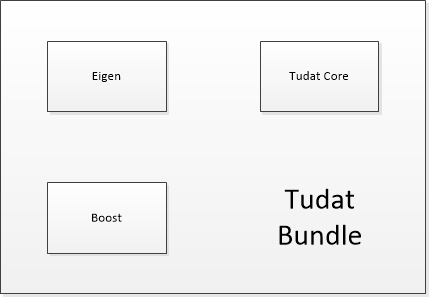
\includegraphics[width=0.3\textwidth]{figures/software/tudatBlock.png}
\caption{\ac{Tudat} structure}
\label{fig:tudatBlock}
\end{figure}

\subsection{Eigen}
\label{subsec:eigen}
Eigen is an external C++ library that was written to perform linear algebra computations \footnote{More documentation on Eigen can be found on \url{eigen.tuxfamily.org/dox/} [Accessed 8 March 2016] }. The software is free and easy to use, which is why it is widely used by the C++ community and thus also within \ac{Tudat} \citep{dirkx2016tudat}. Another advantage is that because it does not use any source files, it does not need to be build before using it. 
The Eigen libraries contain a number of standardized matrices and vectors, each with its own characteristics. An example of an often used vector is \textit{Vector3d} (or \textit{Eigen::Vector3d}), which can for instance be used to store the Cartesian position of a satellite. Here the \textit{3} shows that it can store 3 values/parameters and the \textit{d} shows that these are of the type \textit{double}. It is mentioned on the \ac{Tudat} wiki \citep{dirkx2016tudat} that these Eigen vectors and matrices should only be used if required for linear algebra computations. For ordinary storage, the C++ arrays, vectors and matrices should be used to save both storage and computation time.


\subsection{Boost}
\label{subsec:boost}
Boost is a slightly more complicated set of C++ libraries, where compared to the Eigen library, Boost first has to be compiled before being able to use all of its functionalities. Fortunately, this compiling is performed by \ac{Tudat} automatically when setting it up for the first time. Boost is described as an addition to the standard C++ libraries, thus adding more functionalities \citep{dirkx2016tudat} \footnote{More documentation on Boost can be found on \url{http://www.boost.org/} [Accessed 8 March 2016]}. Within \ac{Tudat}, Boost is used to pass free and class functions as an argument to another object and also for dynamic allocation using so-called pointers. Four libraries that are often used within \ac{Tudat} are \textit{boost::function}, \textit{boost::bind}, \textit{boost::shared\_ptr} and \textit{boost::make\_shared}. The first two libraries are used to pass functions (a function is pointed to by \textit{function} and called by \textit{bind}) and the last two are used in case of dynamic allocation (\textit{shared\_ptr} is the pointer and \textit{make\_shared} is the object creator that returns a shared pointer to the created object). 

\subsection{\ac{PaGMO}}
\label{subsec:pagmo}
\ac{PaGMO} is a free optimisation tool developed by \ac{ESA}s \ac{ACT}. It uses parallel computations to perform the optimisation and can even optimise for multi-objective problems. Parallel computation is the act of performing multiple computations on the same machine using different CPU cores. This allows the cost function to be computed for different sets of optimisation parameters at the same time and thus reducing the total CPU time required. However, this only works if the cost function evaluations are independent, which is not always the case (e.g. Dynamic \ac{DE} described by \cite{qing2009differential}). The tool itself incorporates many different local and global optimisation methods as mentioned by \cite{izzo2012pygmo}, among which the optimisation method used in this thesis \ac{MBH}. This method has been written in \ac{PaGMO} in such a way that it can use any of the provided local optimisers. \ac{PaGMO} is written in C++ and requires the shared libraries of Boost to run \footnote{More documentation on \ac{PaGMO} can be found on \url{https://esa.github.io/pagmo/} [Accessed 9 March 2016]}. Interfaces to external libraries are also provided, which can incorporate for instance \ac{SNOPT} as a local optimisation method. In this thesis \ac{SNOPT} is used as the local optimiser for \ac{MBH} as implemented by \ac{PaGMO}. More information on \ac{SNOPT} is provided in \Cref{subsec:snopt}. For \ac{SNOPT} to be recognised by \ac{PaGMO}, it has to be installed separately. \Cref{fig:pagmoBlock} shows \ac{PaGMO} with the internally used Boost library and the externally called \ac{SNOPT} software.

\begin{figure}[!ht]
\centering
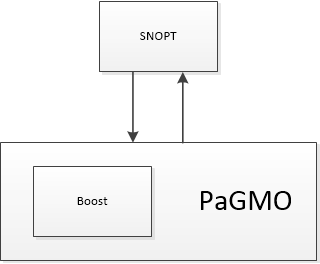
\includegraphics[width=0.3\textwidth]{figures/software/pagmoBlock.png}
\caption{\ac{PaGMO} structure}
\label{fig:pagmoBlock}
\end{figure}

\subsection{\ac{SNOPT}}
\label{subsec:snopt}
\ac{SNOPT} was introduced by \cite{gill2002snopt} as a \ac{SQP} method. It uses the first function derivatives and is very effective with highly constrained problems such as trajectory optimisation. Because it is based on \ac{SQP} it is only able to find  the local optimum and it is thus not guaranteed that this is also the global optimum. By combining \ac{SNOPT} and \ac{MBH} the global optimum can indeed be found or approached. The tool itself does not require that many evaluations, which is why it is very useful for complex problems with many optimisation variables \citep{gill2006user}. The code for \ac{SNOPT} has been written in Fortran, but can easily be translated to C,C++ using \textit{f2c} which is provided with \ac{SNOPT} as well \footnote{More documentation on \ac{SNOPT} can be found on \url{http://www.sbsi-sol-optimize.com/asp/sol_products_snopt_desc.htm} [Accessed 9 March 2016]}. This way it can be called by \ac{PaGMO}. It should be noted that \ac{SNOPT} is not free and can only be used under a licence agreement.

\subsection{Mars-\ac{GRAM}}
\label{subsec:marsgram}
Mars-\ac{GRAM} is a high-fidelity atmospheric model developed by NASA to simulate the global atmospheric conditions on Mars \citep{justus2008utilizing} \footnote{NASA website: \url{https://see.msfc.nasa.gov/model-Marsgram} [Accessed 9 March 2016]}. The model
is based on NASA Ames Mars General Circulation Model (for altitudes between 0-80 km) and Mars Thermospheric General Circulation model (for altitude above 80 km). It can provide density, temperature and pressure data (among other data) with respect to the current altitude, latitude and longitude on Mars.  Seasonal variations are taken into account in the model as well, which is why different calender dates will result in different atmospheric compositions. The tool can be used within a simulation tool or as a separate executable. Unfortunately, because it is so detailed, each computation requires a lot of CPU time. This is why it was decided to use the stand-alone Mars-\ac{GRAM} executable to generate a detailed table with atmospheric data as a function of altitude, latitude and longitude at the start of the optimisation. Even generating this table required a lot of CPU time (on average a single computation using the stand-alone executable took 67.9 seconds to complete). The starting altitude was set at -0.6 km \ac{MOLA} and advanced with a step-size of 0.1 km to 320 km altitude to cover the entire range that the \ac{MAV} would have to cover. Also, the latitude and longitude were varied within 10 degrees from the launch site with a step-size of 1 degree. A Matlab script was written to extract the relevant atmospheric data from the Mars-\ac{GRAM} output files and write them into a .csv file, thus creating the required atmospheric data table. The atmospheric data in this table was then interpolated to provide an estimate of the atmospheric characteristics at every point along the ascent trajectory, which is required to compute the drag at each time step. Some of the earlier versions of Mars-\ac{GRAM} are available for free (such as the Mars-\ac{GRAM} 2005 version used in this thesis), however, the latests versions (such as the Mars-\ac{GRAM} 2010 version used as a back-up in this thesis) require a licence agreement.


\section{Developed software}
\label{sec:developedsoftware}
This section of the software chapter describes the software that either had to be developed around existing software/libraries or had to be developed from scratch (the \ac{TSI} propagator). Each piece of software is accompanied by the corresponding software architecture. Every next piece of software then indirectly incorporates the previous architecture through the use of the completed tool.


%\subsection{Interpolator}
%\label{subsec:interpolatorsoft}
%
%\begin{figure}[!ht]
%\centering
%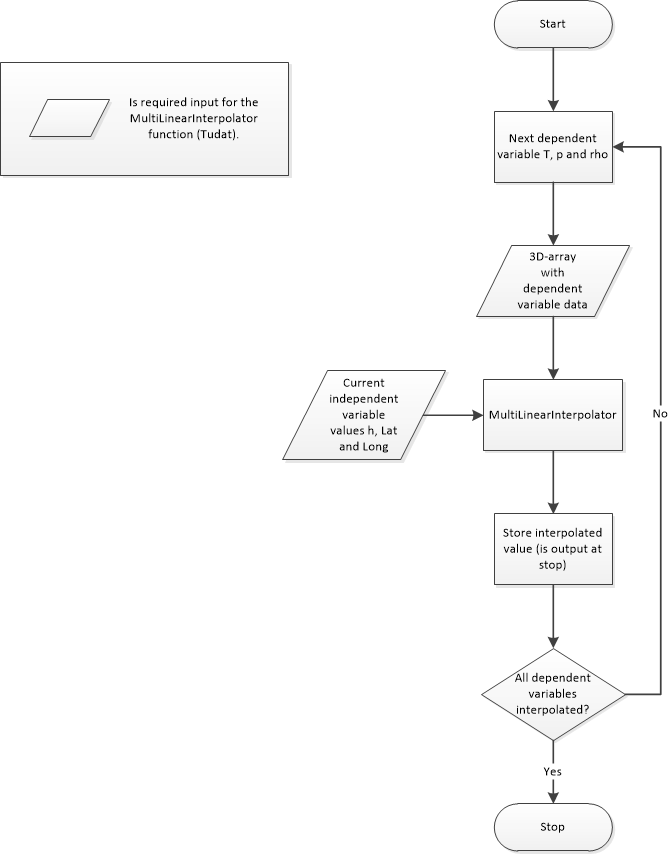
\includegraphics[width=0.5\textwidth]{figures/software/interpolator.png}
%\caption{Interpolator interface architecture}
%\label{fig:interpolator}
%\end{figure}

\subsection{Atmospheric table function fit}
\label{subsec:atmofuncfit}
Using Mars-\ac{GRAM} 2005, a table containing altitude, latitude and longitude dependent temperature and density data was produced. The altitude range was -0.6 to 320 km \ac{MOLA} with a step-size of 0.01 km, the latitude and longitude ranges were centred around the launch site (21.0 $^\circ$N and 74.5 $^\circ$E) with a 10 degree range in each direction and a step-size of 1 degree. The rest of the input parameters were constant and can be seen in \Cref{app:appendixA-marsGRAM-inputFile}. The temperature and density data produced is shown in \Cref{fig:temperatureData,fig:densityData} respectively for 9 latitude and longitude combinations including the launch site itself.                                                                                                                                                                                                                                                                                                                                                                                                                                                                                          


\begin{figure}[!ht]
\centering
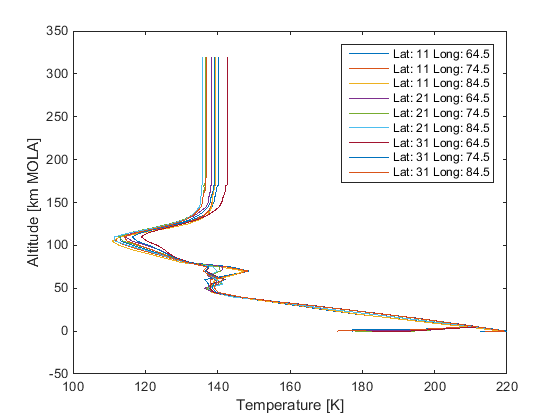
\includegraphics[width=1.0\textwidth]{figures/software/temperatureData.png}
\caption{Temperature data generated with Mars-\ac{GRAM} 2005 showing 9 different latitude and longitude combinations}
\label{fig:temperatureData}
\end{figure}

\begin{figure}[!ht]
\centering
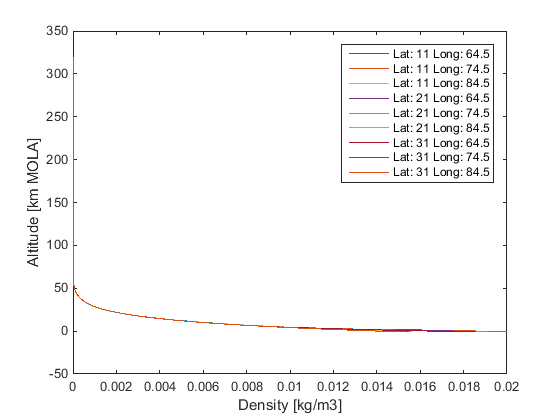
\includegraphics[width=1.0\textwidth]{figures/software/densityData.png}
\caption{Density data generated with Mars-\ac{GRAM} 2005 showing 9 different latitude and longitude combinations}
\label{fig:densityData}
\end{figure}

Unfortunately discontinuous data tables cannot be used when integrating using \ac{TSI}, which is why both these data tables had to be fitted with continuous functions. The temperature data could not be smoothly fit with one continuous function.  Therefore, depending on the altitude range, a different approximation function is required. The condition to be met for a proper fit came from the differences in the temperature-altitude and density-altitude curves, where the maximum difference with respect to the launch site curve was taken. The requirement for the standard deviation of the polynomial curve fit was then to be (at least) one order lower than this maximum difference and that the maximum difference between the fit and the launch site curve was lower than the maximum difference. The temperature-altitude curve was split into 5 sections as roughly visualised in \Cref{fig:temperatureDataSplit5}. The number of sections come from both the shape of the curves and the requirement for accuracy and maximum order of the polynomial, which is set at 8 because otherwise the polynomial would get too long. Also, the number of sections were to be kept at a minimum. More information on the fitting process and early results is provided in \Cref{app:appendixB-fittingProcessAndResults}.

\begin{figure}[!ht]
\centering
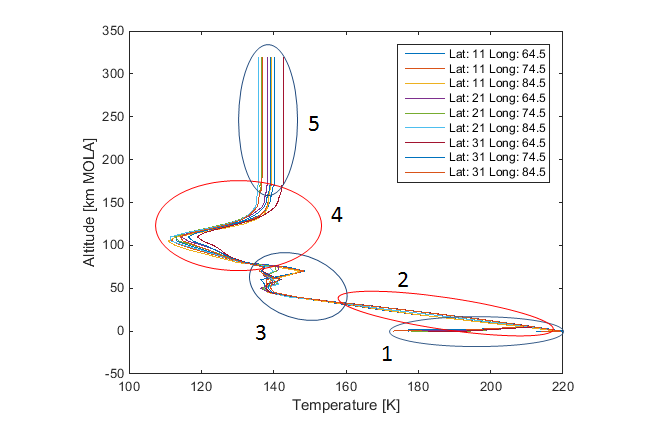
\includegraphics[width=1.0\textwidth]{figures/software/temperatureDataSplit5.png}
\caption{Different temperature curve sections}
\label{fig:temperatureDataSplit5}
\end{figure}

Each section was fit with a polynomial function of the n$^{th}$ order where the function is represented by \Cref{eq:polyGenFunct}. The last section shows a constant temperature, thus the temperature of the launch site curve was chosen to represent this final section, which is equal to 136.5 K.

\begin{equation} \label{eq:polyGenFunct}
y=p_{n}x^{n}+p_{n-1}x^{n-1}+\dots+p_{1}x+p_{0}
\end{equation}

A lower order is preferred, because then the fitted function will be simpler to evaluate and contain fewer terms. However the order has to be high enough to meet the accuracy requirements. \Cref{tab:fitDeviations} shows the orders that were required and the deviations to the launch site temperature-altitude curve. The actual corresponding parameters are provided in \Cref{tab:fitParameters}. It should be noted that the first few temperature data values were so different from the rest of the curve that it was assumed that this is a lack of the Mars-\ac{GRAM} program and were thus treated as outliers.

\begin{table}[!ht]
\begin{center}
\caption{Temperature curve fit data all with respect to the launch site curve (Latitude and longitude of the launch site)}
\label{tab:fitDeviations}
\begin{tabular}{|l|l|l|p{3cm}|p{3cm}|p{3cm}|}
\hline 
\textbf{Section} & \textbf{Altitude range [km MOLA]} & \textbf{Order}	& \textbf{Maximum polynomial standard deviation [K]} & \textbf{Maximum polynomial difference [K]} & \textbf{Maximum data curves difference [K]} \\ \hline 
1 & -0.6 to 5.04 & 1 & 0.0312 & 25.8 & 0.177 \\ \hline
2 & 5.04 to 35.53 & 2 & 0.287 & 3.90 & 0.7056 \\ \hline
3 & 35.53 to 75.07 & 6 & 0.624 & 8.00 & 1.69 \\ \hline
4 & 75.07 to 170.05 & 8 & 0.523 & 6.60 & 2.45 \\ \hline
\end{tabular}
\end{center}
\end{table}

\begin{table}[!ht]
\begin{center}
\caption{Temperature curve fit parameters (rounded to 3 decimal points)}
\label{tab:fitParameters}
\begin{tabular}{|l||p{1.1cm}|p{1.1cm}|p{1.1cm}|p{1.1cm}|p{1.1cm}|p{1.1cm}|p{1.1cm}|p{1.1cm}|p{1.1cm}|}
\hline 
\textbf{Section}  & $\mathbf{p_{8}}$ & $\mathbf{p_{7}}$ & $\mathbf{p_{6}}$ & $\mathbf{p_{5}}$ & $\mathbf{p_{4}}$ & $\mathbf{p_{3}}$ & $\mathbf{p_{2}}$ & $\mathbf{p_{1}}$ & $\mathbf{p_{0}}$ \\ \hline 
1 &  &  &  &  &  &  & & 3.415 & 194.165   \\ \hline
2 &  &  &  &  &  & & 0.006 & -2.130 & 222.052   \\ \hline
3  &  &  & -5.388 $\cdot$10$^{-7}$ & 1.785 $\cdot$10$^{-4}$ & -0.0243 & 1.733 & -68.294 & 1.407 $\cdot$10$^{3}$ & -1.167 $\cdot$10$^{4}$ \\ \hline
4  & 4.1942 $\cdot$10$^{-12}$ & -4.328 $\cdot$10$^{-9}$ & 1.931 $\cdot$10$^{-6}$ & -4.862 $\cdot$10$^{-4}$ & 0.076 & -7.405 & 447.378 & -1.523 $\cdot$10$^{4}$ & 2.236 $\cdot$10$^{5}$ \\ \hline
\end{tabular}
\end{center}
\end{table}

The complete polynomial fit for the launch site curve for the temperature is shown in \Cref{fig:completePolyFitTempSplit5}.

\begin{figure}[!ht]
\centering
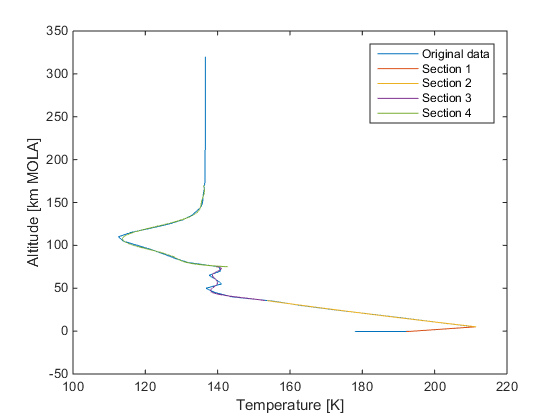
\includegraphics[width=1.0\textwidth]{figures/software/completePolyFitTempSplit5.png}
\caption{All section fits for the launch site temperature data curve}
\label{fig:completePolyFitTempSplit5}
\end{figure}




The density fit was slightly more difficult because the curves are all very similar and thus result in a higher accuracy requirement for the fit. At first glance it looks like a natural logarithmic function, unfortunately an ordinary exponential did not fit the curve. This is why a more extensive exponential fit was required. The natural logarithm of the data has been plotted in \Cref{fig:lnPlotDataDen}.

\begin{figure}[!ht]
\centering
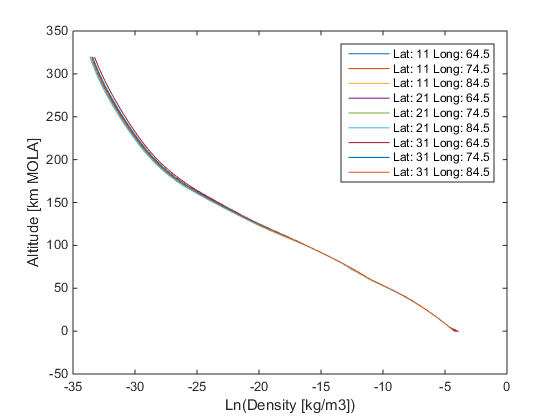
\includegraphics[width=1.0\textwidth]{figures/software/lnPlotDataDen.png}
\caption{Natural logarithmic plot of the density data}
\label{fig:lnPlotDataDen}
\end{figure}

With the data represented in the logarithmic domain, again a polynomial function can be fit. The total fit would then satisfy \Cref{eq:expPoly}.

\begin{equation} \label{eq:expPoly}
y=exp\left( p_{n}x^{n}+p_{n-1}x^{n-1}+\dots+p_{1}x+p_{0}\right)
\end{equation}



% A logarithmic fit (such as an exponential atmosphere) resulted in a lower overall accuracy than the polynomial fits. In this case the curve was split into three sections, because the differences between the curves were bigger in the lower atmosphere. These sections are illustrated in \Cref{fig:densityDataSplit3}.
%
% \begin{figure}[!ht]
%\centering
%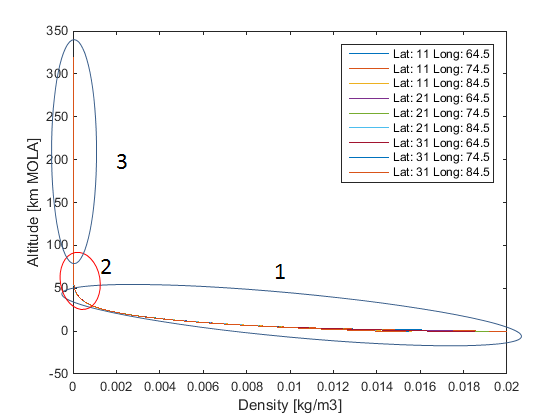
\includegraphics[width=1.0\textwidth]{figures/software/densityDataSplit3.png}
%\caption{Different density curve sections}
%\label{fig:densityDataSplit3}
%\end{figure} 

The same polynomial requirements as for the temperature curve were enforced for the density curve as well. However, because the polynomial is used in an exponential, some extra requirements are needed to assure the accuracy of the fit. One requirement is that the maximum difference between the final exponential fit and the normal launch site density curve is smaller than the maximum difference between all the data curves. Also, in this case the standard deviation of the difference between the exponential fit and the normal launch site curve had to be within the range of standard deviations of the difference between the different data curves. This meant that even though an 8$^{th}$ order polynomial fit could be achieved for the natural logarithmic data with the required accuracy, when converted to the exponential fit, the last two requirements were not met. Before it was mentioned that an order higher than 8 was not desirable. However, in this case, a single exponential fit could be achieved using a 10$^{th}$ order polynomial. This fit meant that the density curve did not have to be split up at all, which makes the integration slightly easier. Therefore, it was decided that a 10$^{th}$ order polynomial was acceptable in this case. The results of the fit is presented in \Cref{tab:fitDeviationsDen,tab:fitParametersDen} and the polynomial and exponential fit curves are shown in \Cref{fig:completeExpPolyFitDen,fig:completeExpFitDen} respectively.

%
% This results in the density polynomial fit data and the polynomial parameters as presented in \Cref{tab:fitDeviationsDen,tab:fitParametersDen} respectively. 

%\textbf{\textcolor{red}{UPDATE THE NEXT TWO TABLE VALUES TO THE VALUES FOR DENSITY!!!}}

%\begin{table}[!ht]
%\begin{center}
%\caption{Density curve fit data (10$^{th}$ order polynomial)}
%\label{tab:fitDeviationsDen}
%\begin{tabular}{|p{3cm}|p{3cm}|p{3cm}|p{3cm}|p{3cm}|p{3cm}|p{3cm}|}
%\hline 
%\textbf{Maximum polynomial standard deviation [kg/m$^{3}$]} & \textbf{Maximum natural logarithmic curves difference [kg/m$^{3}$]} & \textbf{Maximum polynomial difference with natural logarithmic launch site curve [kg/m$^{3}$]} & \textbf{Maximum curves difference [kg/m$^{3}$]} & \textbf{Maximum difference with launch site curve [kg/m$^{3}$]} & \textbf{Maximum standard deviation curves difference [kg/m$^{3}$]} & \textbf{Standard deviation exponential fit difference [kg/m$^{3}$]} \\ \hline 
%0.0501 & 0.460 & 0.160   & 3.910$\cdot$10$^{-3}$ &  2.826$\cdot$10$^{-3}$ & 2.106$\cdot$10$^{-4}$ & 1.167$\cdot$10$^{-4}$ \\ \hline
%
%\end{tabular}
%\end{center}
%\end{table}

\begin{table}[!ht]
\begin{center}
\caption{Density curve fit data (10$^{th}$ order polynomial) with respect to the launch site curve (Latitude and longitude of the launch site)}
\label{tab:fitDeviationsDen}
\begin{tabular}{|l|l|}
\hline 
\textbf{Maximum polynomial standard deviation [kg/m$^{3}$]} & 0.0501 \\ \hline

  \textbf{Maximum polynomial difference [kg/m$^{3}$]} & 0.160 \\ \hline
  
   \textbf{Maximum natural logarithmic data curves difference [kg/m$^{3}$]} & 0.460 \\ \hline
  
    \textbf{Maximum exponential difference with launch site curve [kg/m$^{3}$]} & 2.826$\cdot$10$^{-3}$ \\ \hline
    
       \textbf{Maximum data curves difference [kg/m$^{3}$]} & 3.910$\cdot$10$^{-3}$ \\ \hline
    
      \textbf{Standard deviation exponential fit difference [kg/m$^{3}$]} & 1.167$\cdot$10$^{-4}$ \\ \hline 
      
           \textbf{Maximum standard deviation data curves difference [kg/m$^{3}$]} & 2.106$\cdot$10$^{-4}$ \\ \hline
\end{tabular}
\end{center}
\end{table}



\begin{table}[!ht]
\begin{center}
\caption{Density curve fit parameters (rounded to 3 decimal points)}
\label{tab:fitParametersDen}
\begin{tabular}{|p{1.1cm}|p{1.1cm}|p{1.1cm}|p{1.1cm}|p{1.1cm}|p{1.1cm}|p{1.1cm}|p{1.1cm}|p{1.1cm}|p{1.1cm}|p{1.1cm}|}
\hline 
 $\mathbf{p_{10}}$ & $\mathbf{p_{9}}$ & $\mathbf{p_{8}}$ & $\mathbf{p_{7}}$ & $\mathbf{p_{6}}$ & $\mathbf{p_{5}}$ & $\mathbf{p_{4}}$ & $\mathbf{p_{3}}$ & $\mathbf{p_{2}}$ & $\mathbf{p_{1}}$ & $\mathbf{p_{0}}$ \\ \hline 
2.287 $\cdot$10$^{-21}$  & -3.724 $\cdot$10$^{-18}$ & 2.559 $\cdot$10$^{-15}$ & -9.620 $\cdot$10$^{-13}$ & 2.146 $\cdot$10$^{-10}$ & -2.884 $\cdot$10$^{-8}$ & 2.273 $\cdot$10$^{-6}$ & -9.604 $\cdot$10$^{-5}$ & 1.414 $\cdot$10$^{-3}$ & -0.0962 & -4.172\\ \hline
\end{tabular}
\end{center}
\end{table}

%The complete polynomial fit for the launch site curve for the density is shown in \Cref{fig:completePolyFitDen}.


\begin{figure}[!ht]
\centering
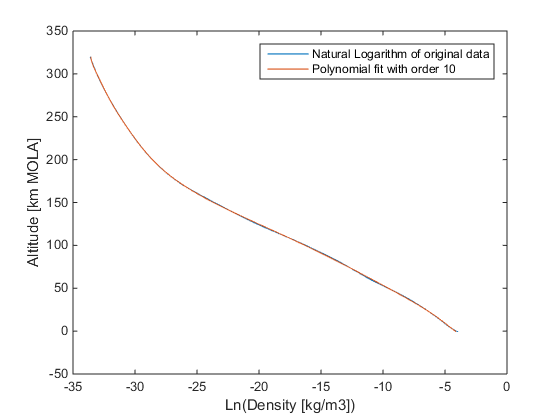
\includegraphics[width=1.0\textwidth]{figures/software/completeExpPolyFitDen.png}
\caption{Polynomial fit for the launch site density data curve}
\label{fig:completeExpPolyFitDen}
\end{figure}

\begin{figure}[!ht]
\centering
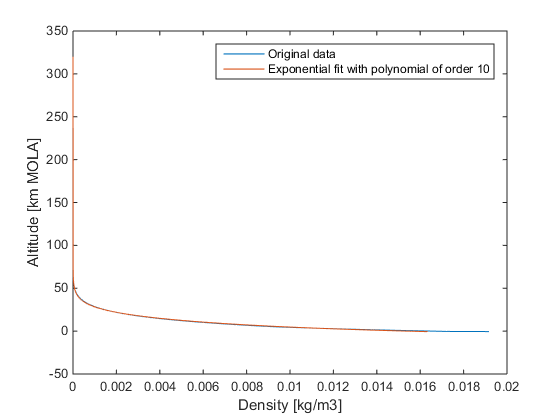
\includegraphics[width=1.0\textwidth]{figures/software/completeExpFitDen.png}
\caption{Exponential fit for the launch site density data curve}
\label{fig:completeExpFitDen}
\end{figure}


%\begin{figure}[!ht]
%\centering
%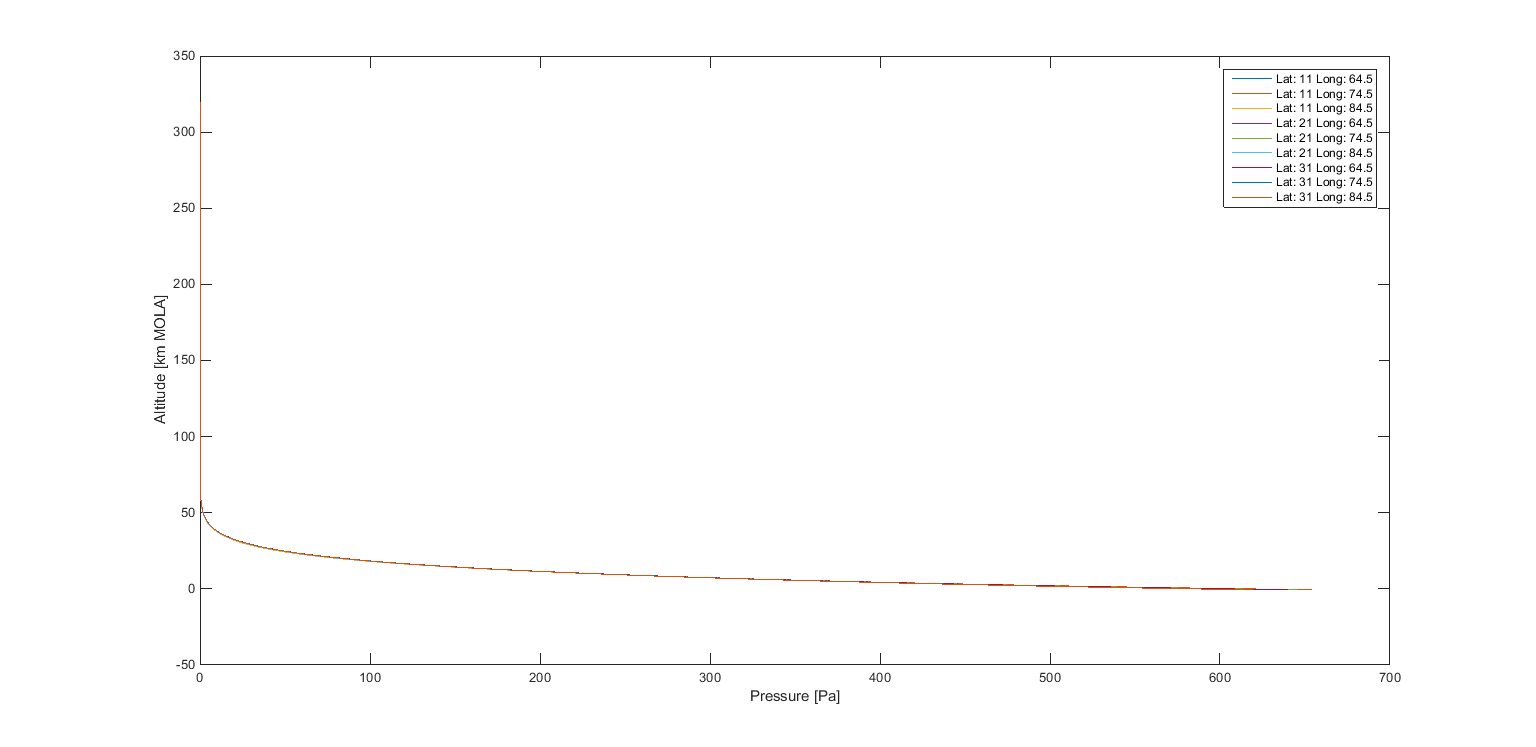
\includegraphics[width=1.0\textwidth]{figures/software/pressureData.png}
%\caption{Pressure data generated with Mars-\ac{GRAM} 2005 showing 9 different latitude and longitude combinations}
%\label{fig:pressureData}
%\end{figure}

\subsection{Drag coefficient graph function fit}
\label{subsec:dragCoefFuncFit}
Similar to the temperature and density curves, the relation between Mach number and drag coefficient, as depicted in \Cref{fig:dragcoeff_whitehead2004mars}, had to be modelled as a continuous function as well. Again, it could not be fitted using one continuous function, but instead had to be modelled by different functions.

\begin{figure}[!ht]
\centering
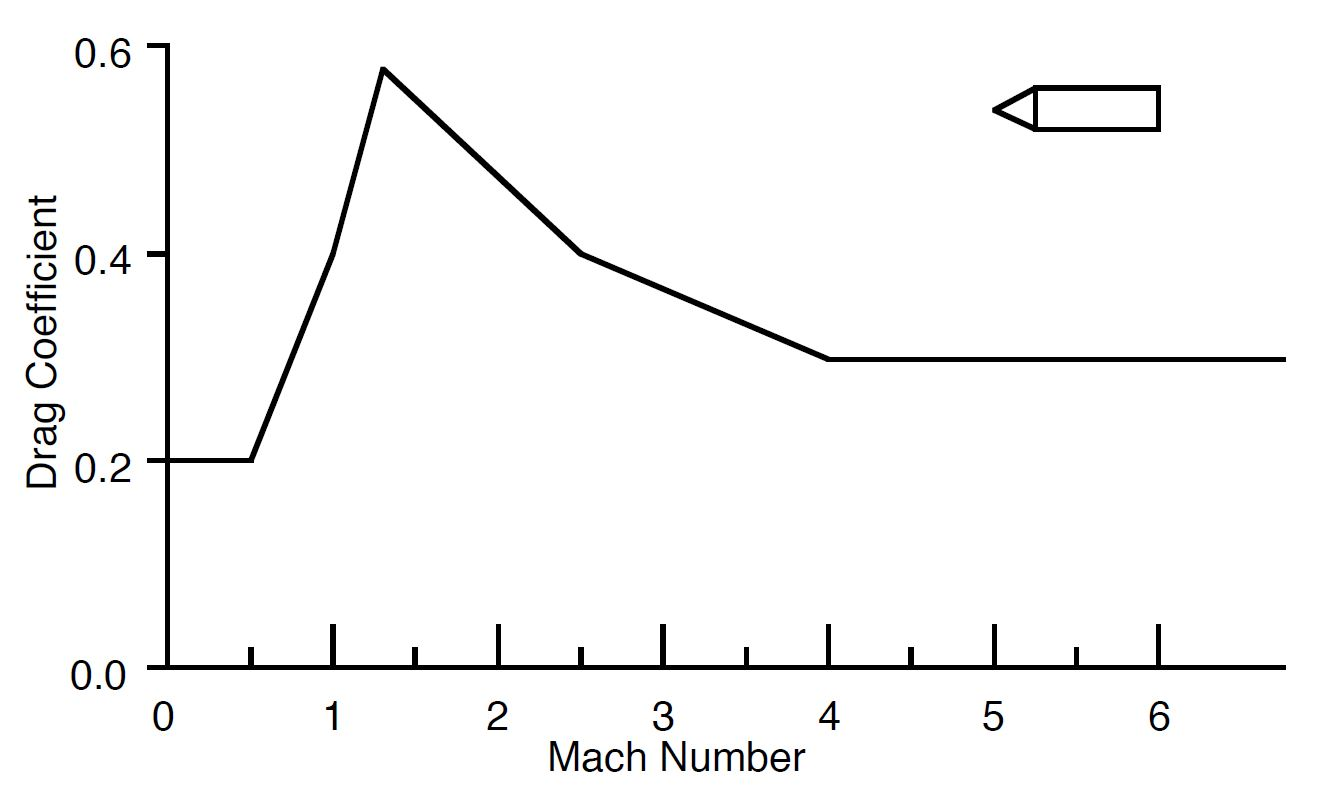
\includegraphics[width=1.0\textwidth]{figures/launcher_methods/dragcoeff_whitehead2004mars.jpg}
\caption{Drag coefficient as a function of Mach number \cite{whitehead2004mars}}
\label{fig:dragcoeff_whitehead2004mars}
\end{figure}

Fortunately, this curve is already an approximation and thus consists of linear elements only. It can be split up into 6 different sections where the first and last section are constant ($C_{D}$ is 0.2 and 0.3 respectively). Using a similar polynomial fit as before, but now for 1 order only, a linear fit could be made for each of the remaining 4 sections. The corresponding parameters are shown in \Cref{tab:dragCoeffPara} and the curve fit is shown in \Cref{fig:dragCoeffFit}.


\begin{table}[!ht]
\begin{center}
\caption{Drag coefficient curve fit parameters (rounded to 3 decimal points)}
\label{tab:dragCoeffPara}
\begin{tabular}{|l|l||l|l|}
\hline 
\textbf{Section}  & \textbf{Mach range}& $\mathbf{p_{1}}$ & $\mathbf{p_{0}}$ \\ \hline 
2  & 0.5 to 1  & 0.400 & -2.483 $\cdot$10$^{-16}$  \\ \hline
3  & 1 to 1.3  & 0.567 & -0.167  \\ \hline
4  &  1.3 to 2.5 & -0.142 & 0.754 \\ \hline
5  &  2.5 to 4 & -0.0667 & 0.567 \\ \hline
\end{tabular}
\end{center}
\end{table}



\begin{figure}[!ht]
\centering
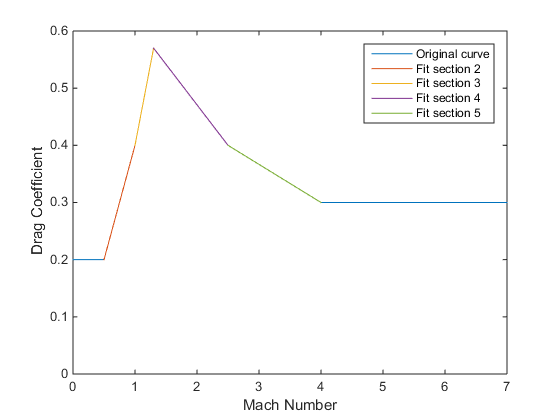
\includegraphics[width=1.0\textwidth]{figures/software/dragCoeffFit.png}
\caption{All section fits for the drag coefficient - Mach curve}
\label{fig:dragCoeffFit}
\end{figure}




\subsection{\ac{RK4} and \ac{RKF} propagator}
\label{subsec:rkpropagator}
The \ac{RK4} and \ac{RKF} (or traditional) propagator architecture is described in \Cref{fig:RK_Propagator}. It starts with the current state, which is then passed on to the state derivative function. The state derivative function is used by the \ac{RK4} and \ac{RKF} integrators to determine the next state by calling the function a number of times depending on the used method. Both \ac{RK4} and \ac{RKF45} (and higher order \ac{RKF} integrators) are already available through the \ac{Tudat} libraries. \ac{RK4} can be called by including the rungeKutta4Integrator.h header file, and \ac{RKF45} can be called by including the rungeKuttaVariableStepSizeIntegrator.h header file. This integration process is repeated until the final condition is met. Within the state derivative function all the sate derivatives are updated and stored. The current position is used to update the gravitational acceleration on the \ac{MAV}, the current mass is used to determine the accelerations caused by the thrust and finally the complete state is required to determine the accelerations caused by the drag. Both the drag and thrust accelerations have to be transformed to the inertial frame using the updated angles from the current state. The function also computes the current mass flow rate, however since the thrust is constant, this does not change over time. In the state derivative function, all the transformations are governed by pre-developed functions within the \ac{Tudat} library, which includes the state transformations and the frame transformation from the body frame to the inertial frame. The transformation from the propulsion frame to the body frame is however not included in \ac{Tudat} and had to be written.


\begin{figure}[!ht]
\centering
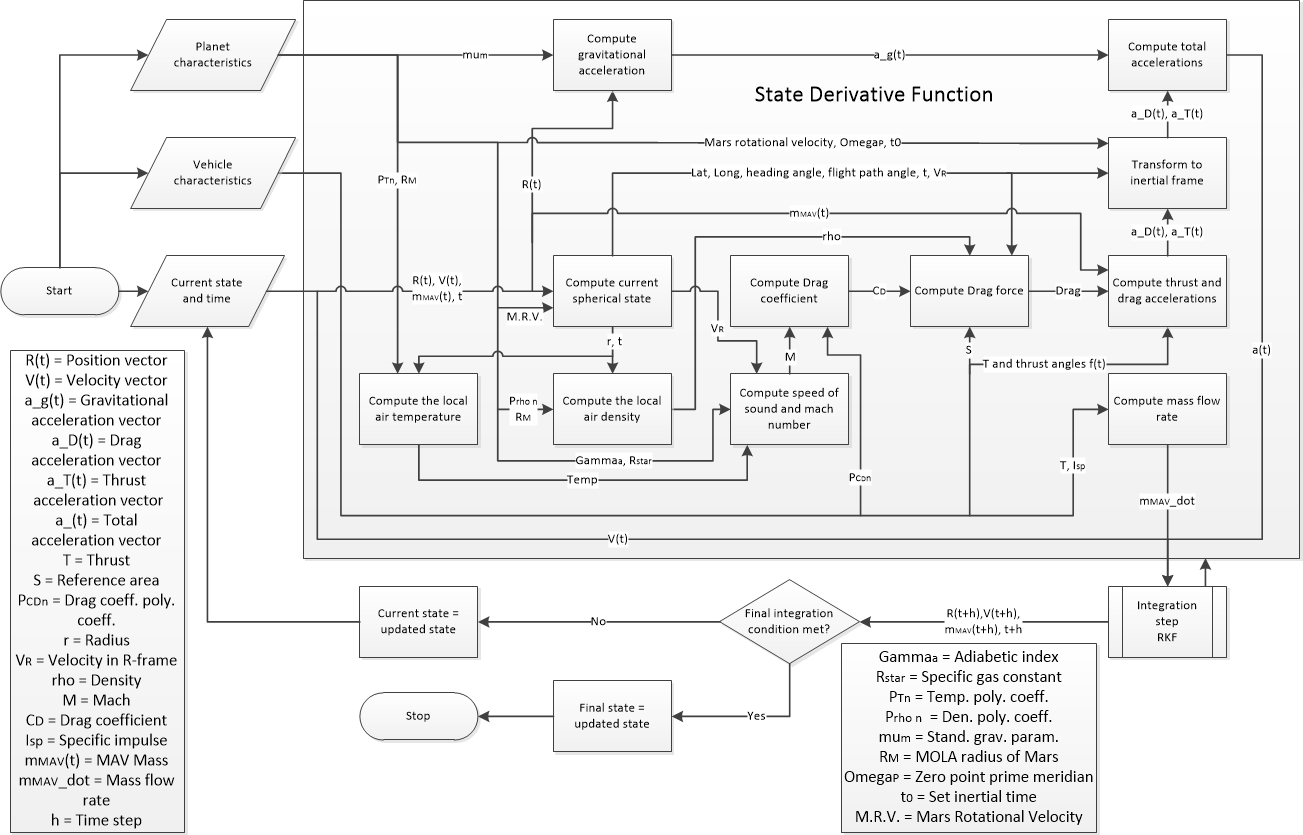
\includegraphics[width=1.5\textwidth, angle = 90]{figures/software/RK_Propagator.png}
\caption{\ac{RK4} and \ac{RKF} interface architecture}
\label{fig:RK_Propagator}
\end{figure}

All blocks represent a different action. These actions might be performed in classes, header files and/or source files. More information on the classification of the different blocks can be found in \Cref{app:appendixC-programFileDefinitions}.

\subsection{\ac{TSI} propagator}
\label{subsec:tsipropagator}
The \ac{TSI} propagator has a significantly different architecture compared to the traditional propagator as can be seen in \Cref{fig:TSI_Propagator}. \ac{TSI} requires an initial order and step-size to start the integration process. In this thesis it has been decided to keep the order the same throughout the entire integration. The step-size will change during the integration depending on the Taylor series evaluations. The initial state is set as the current state and is fed into the \ac{TSI} block. Within this block, first the auxiliary equations and functions are called, which were set-up for this particular problem. They are evaluated using the current state. These auxiliary equations and functions already include all the reference frame and coordinate transformations, as well as approximate atmospheric parameter functions. This is required to set-up the recurrence relations, which is where \ac{TSI} differs from the traditional propagator. Once the auxiliary equations and functions have been computed they are used to compute the Taylor coefficients through the recurrence relations set-up for the thesis problem. These coefficients are then stored for later use and are also passed to the block creating the Taylor series expansion for every state variable thus creating he updated state. The last two coefficients are then used to determine the next step-size. This continues until the final integration condition has been met. 


\begin{figure}[!ht]
\centering
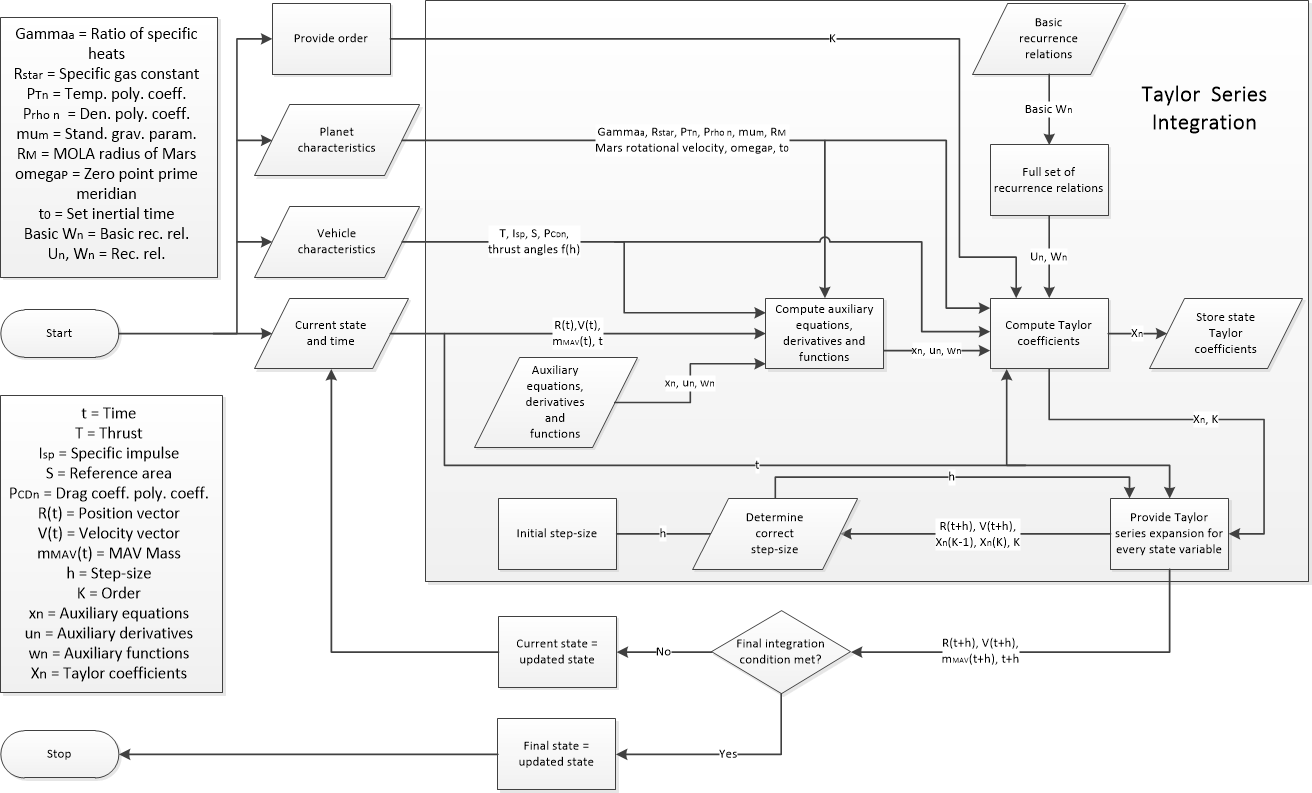
\includegraphics[width=1.5\textwidth, angle = 90]{figures/software/TSI_Propagator.png}
\caption{\ac{TSI} architecture}
\label{fig:TSI_Propagator}
\end{figure}


\subsection{Optimiser}
\label{subsec:optimisersoft}
The optimisation software is a combination of the \ac{SNOPT} local optimisation tool and \ac{PaGMO}s \ac{MBH}. Even though both these tools were already available and did not have to be developed, it is still important to understand how the rest of the software interacts with the optimiser. This is why  \Cref{fig:optimiser} shows the architecture of the \ac{MBH} optimiser. It starts with the initial generation of the optimisation parameters, after which the 'Number of not improved iterations' is set to zero. This is then fed into the local optimiser, where the trajectory is integrated using the previously described tools. Once a local optimised trajectory is found, it is stored if it is better than the previous local optimised trajectory and the counter is set to zero again. If the newly found trajectory is not better than the current best the 'Number of not improved iterations' is increased by one. Once the maximum number of not improved iterations is met, the current best optimal trajectory (which is the optimum for the current "funnel") is stored and the process is repeated till the final global optimisation condition is met. At this point the global optimum is the best optimal trajectory from all the funnels computed at that time, which is then returned as the program solution.

\begin{figure}[!ht]
\centering
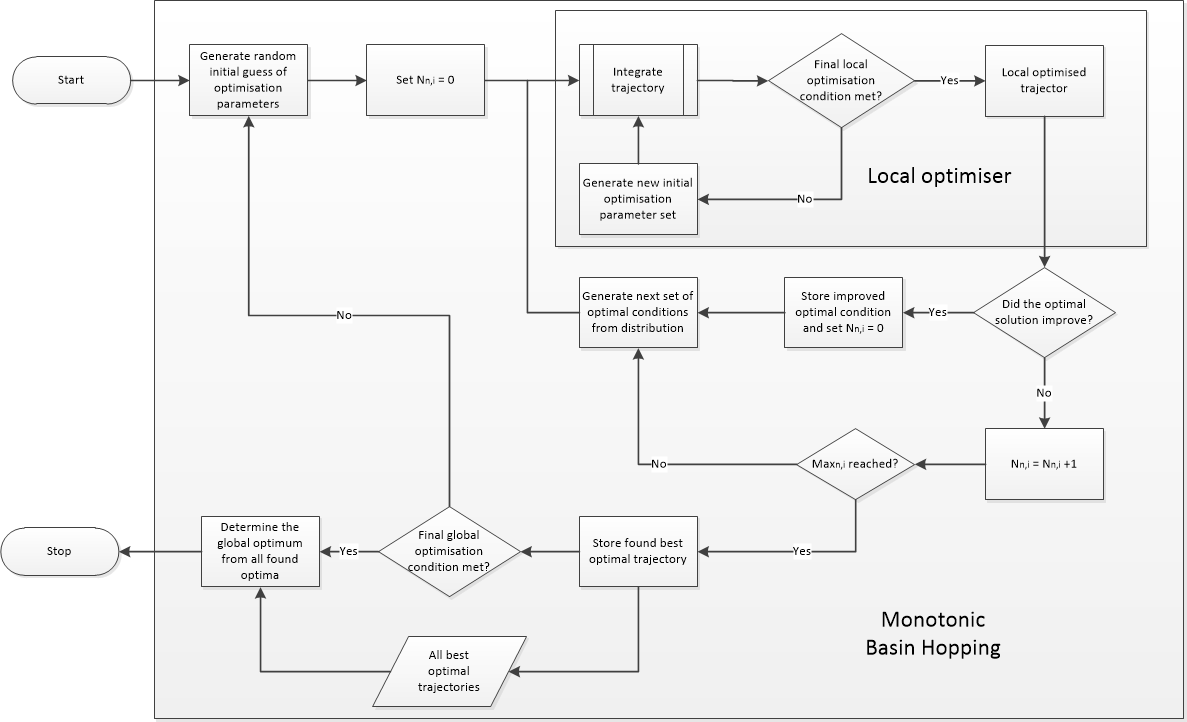
\includegraphics[width=1.5\textwidth, angle = 90]{figures/software/optimiser.png}
\caption{Optimiser interface architecture}
\label{fig:optimiser}
\end{figure}


%\section{Architectures}
%\label{sec:architecture} % For thesis

\chapter{Verification and validation} 
%Last updated 10-03-2016
% Updated 21-10-2016 Got rid of optimisation and added to RKF. Also wrote the TSI part but should still focus on the change in models when writing the complete tool verification and validation including the different test cases.
% Updated 07-11-2016 Small changes to TSI text and wrote the third section on the complete propagation tool.
% Updated 10-11-2016 added sub-section on the validation of the complete tool
% Updated 14-11-2016 continued work on validation section; including the validation cases of Ryan and Joel.
\label{ch:verificationandvalidation}
Verification is the process of determining whether a program meets the requirements or not. Is it working the way it is suppose to? As soon as it works and produces output (verified), these outputs can be compared to other data from which it is known that it is correct. This is called validation. If a program is verified and validated, the outputs should be correct. Fortunately, all the existing software has already been validated, which means that they only still have to be verified to make sure everything is working properly on the simulation computer. Each of the software packages comes with tests which can be used to do this. If all the tests are passed it means that the software is verified for the computer and ready to use. Since \ac{Tudat} shipped with Eigen and Boost, the \ac{Tudat} test files also test these libraries. All the tests were passed, which means that the \ac{Tudat}, Eigen and Boost libraries are working properly. However, because the integrators are an intricate part of this thesis, it was decided to perform a separate verification for the Runge-Kutta integrators. This verification is described in \Cref{sec:rkandrkfver}.

 Mars-\ac{GRAM} also came with its own verification test, where three delivered output files had to be replicated. These verification tests were also successful. 


\section{\acs{RK4} and \acs{RKF} integrators}
\label{sec:rkandrkfver}
The tutorial page of the \ac{Tudat} website \citep{dirkx2016tudat} offers two integration tutorials: one involving \ac{RK4} and another involving variable step-size Runge-Kutta methods including \ac{RKF}. The objective of the tutorial is to get familiar with the different integration methods available in \ac{Tudat}. At the same time, a small data table has to be reproduced, which also serves as a verification test. For each of the integrators the same problem was addressed: the computation of the velocity of a falling body after a certain amount of time assuming no drag. The results that had to be reproduced are presented in \Cref{tab:intverdat}.


\begin{table}[!ht]
\begin{center}
\caption{Verification data for the standard integrators}
\label{tab:intverdat}
\begin{tabular}{|l|l|l|l|l|}
\hline 
\textbf{End time [s]} & 1.0	& 5.0 & 15.0 & 25.0 \\ \hline 
\textbf{Velocity [m/s]} & -9.81 & -49.05 & -147.15 & -245.25 \\ \hline
\end{tabular}
\end{center}
\end{table}

The first script was written using the instructions from the tutorial and is called numericalintegrators.cpp. This script uses the rungeKutta4Integrator.h header file and the RungeKutta4IntegratorXd function from this header file. This function requires three inputs: the state derivative function (problem specific), the initial time and the initial state. Using the .integrateTo extension the end state at a certain end time can be computed. This requires the end time and the step-size. For \ac{RK4} the step-size is constant. This resulted in the same values as presented in \Cref{tab:intverdat}.\\

The second script was used to test the variable step-size integrators \ac{RKF}. This script is called rungekuttavariable.cpp and uses the rungeKuttaCoefficients.h and rungeKuttaVariableStepSizeIntegrator.h header files. In this case the RungeKuttaVariableStepSizeIntegratorXd function was used which requires the Runge-Kutta coefficients (from the respective header file), the state derivative function (problem specific), the initial time, initial state, zero minimum step-size, infinite maximum step-size, relative tolerance and the absolute tolerance as inputs. In this case the integration can be done in individual steps using .performIntegrationStep with the current step-size as the only input. The current step-size is computed in the integration method itself, but in this case it is checked to make sure that the step-size does not take the function beyond the specified end time. The integration steps are then repeated until the end time is met. Running this script resulted in the same results as presented in \Cref{tab:intverdat} as well. \\

These results, combined with the fact that the test files for these two methods produced no errors is proof that they are working accordingly. Thus it can be said that the standard integration methods used in this thesis are verified and ready for use in the simulation tool. However, during the development of the trajectory propagation tools, the entire tool (including the integrators) will be verified again to determine the performance of the integrators.

For the actual propagation tool, the \ac{RKF} method required the state derivative function associated with this particular ascent problem. The state derivative class was constructed using the state derivative functions as described in this thesis in the Cartesian coordinate system based on equations provided by \cite{mooij1994motion}. The state is used to compute the required transformation angles first and then both the thrust and drag accelerations are transformed to the inertial frame. There they are combined with the gravitational acceleration resulting in the accelerations in the x-, y- and z-direction. This class was tested by itself by inputting certain values which would result in known outcomes. And those simple values by themselves provided the expected results. Later the state derivative function was combined with the \ac{RKF} integrator in the trajectory propagation tool and verified again as will be described in \Cref{sec:propverval}. 


The verification of the state derivative class took approximately one day. 



\section{\acl{TSI}}
\label{sec:tsiverval}
In this section, the verification and validation of the \ac{TSI} header and source file is described. This was done for each of the blocks shown in \Cref{fig:TSI_Propagator}. For the verification it was important that the running of the different classes and header/source files did not produce any obvious errors. For the validation, the results were often checked against manual calculations and expected behaviour. The verification and validation of \ac{TSI} was a very lengthy process and required many rewrites of the used equations because of mistakes in the model or mistakes in the derivations. \Cref{sec:propverval} talks a bit more about the model mistakes. This section has been divided into several subsections which showed similar issues during the verification and validation.

\subsection{Auxiliary equations, derivatives and functions}
\label{subsec:auxEqDerFunverval}
As shown by \Cref{fig:TSI_Propagator} the first step in the \ac{TSI} is to compute the auxiliary equations, derivatives and functions. The computations, in theory, are fairly straightforward, however it is really easy to make a mistake. During the initial verification of these different classes the outcomes were checked against simple manual solutions. Thus, provided a certain input, the output was known. This was an easy way to check any coding errors. Since the early versions of the code required a lot of equations, it took a long time to go through all the equations and find all the errors and mistakes. This was initially done with the combination of Cartesian coordinates and spherical transformation angles, however, later on more efficient equations were used for separate Cartesian and spherical cases. This also made it easier to identify mistakes in the equations and understand certain issues found during the validation process. 

\subsection{Computing the Taylor Series coefficients and the updated state}
\label{subsec:TaySerCoefverval}
Once the auxiliary classes were verified, the Taylor Series coefficients could be computed using the basic recurrence relations and the full set of recurrence relations. For the Taylor Series coefficients it is important that they show a decreasing number series for each of the coefficients. This was the desired outcome that was used for the verification of the full set of recurrence relations. The basic recurrence relations were all checked by hand calculations to determine if they indeed worked the way that they were suppose to. The verified basic recurrence relations were used to verify the full set of recurrence relations. This class consists of the equations mentioned in \Cref{app:appendixD-allRecurrenceRelations}. When writing the full set of recurrence relations, it is really easy to make mistakes and there are a lot of rules that have to be taken into account as mentioned in \Cref{ch:tsi}. Therefore, a lot of time was spend on rewriting these equations in such a way that the outcomes were what was expected. Also, a number of these recurrence relations were checked by manual calculations. An often recurring problem was that the Taylor Series coefficients would show a diverging behaviour where the coefficient would keep increasing to infinity (theoretically). This was often an indication that a writing mistake was made when setting up the full set of recurrence relations. Another easy way to identify mistakes during the validation process was to compute the next state. Should an error occur in the computation of the Taylor Series coefficients, this would usually result in very large increases in the state even if the coefficient itself would be relatively small. Then following the trail back to the largest change in Taylor Series coefficient, often a coding or writing mistake could be identified in the full set of recurrence relations. 

\subsection{Next step-size}
\label{subsec:nextStepSizeverval}
Fortunately, the step-size class was not a very large class and took less time to verify and validate. Provided a set of Taylor Series coefficients, the step-size class could be tested separately from the other files. The verification process was rather straight forward; the class should be able to provide a step-size estimate given the different input values. Also, when similar sets of Taylor Series coefficients were used, the output step-sizes should be rather similar. This was then also part of the validation process. A pure validation process was difficult because there were no reference Taylor series coefficients available, however an estimate for the order of the next step-size could be used. This can however still be improved. Two different step-size determination methods were tested, but in the end it was found that the direct method described by \cite{scott2008high} and \cite{bergsma2015application} showed more reasonable results and was easier to implement. Also, during the verification process, the iteration method failed to work properly which led to unusable results and the program failing. But the direct method worked very well.




\section{Complete trajectory propagation}
\label{sec:propverval}
For the complete trajectory propagation it was important to have the integrator method as the only difference between the \ac{RKF} and the \ac{TSI} propagation. First the initial values were provided and transformed into the proper coordinate system. These would then be fed into the integrator and at the end of the integration, the results would be printed. The verification and validation of the complete trajectory propagation have been split up into several phases.


\subsection{Phase 1: \ac{RKF} propagation}
\label{subsec:phase1com}
This was first done for \ac{RKF} because this method was already validated. Therefore, any mistakes or problems found would lead back to a mistake in the state derivative functions or the model itself.
During this phase, a number of problems were identified; certain singularities were found, a limit to the tolerance value was determined for each of the \ac{RKF} methods (\ac{DOPRIN87} does not converge fast enough in many cases for a value of 10$^{-15}$) and a mistake in the model was found where the wrong velocity was used to determine the drag acceleration. This meant that some of the model equations had to be rewritten for both \ac{RKF} and \ac{TSI}. 

\subsection{Phase 2: both \ac{RKF} and \ac{TSI}}
\label{subsec:phase2com}
During the second phase of the verification, both \ac{RKF} and \ac{TSI} were tested at the same time and the outcomes were compared. Since the \ac{RKF} method was verified and validated at this point, the outcome of the \ac{RKF} propagation could be used to verify \ac{TSI}. This was done using different test cases that focussed on different elements of the code. 

Each element was tested separately by activating (or deactivating) the gravity, thrust and drag as well as the rotation of Mars. In each case, simple test cases were used to verify the class, such as: vertical drops from a certain altitude, thrusting in a known direction and flying parabolic trajectories. This was all done in each of the axis directions first and then combining the different axes. First the gravity was tested, then the thrust, then a combination of these two, followed by the drag all in the non-rotating case. The same was then done for the rotating case as well. This was initially done for a zero thrust elevation and thrust azimuth angle, such that the trust was acting directly through the x-axis of the body frame. Also, because the drag by definition works through the x-axis of the body frame, there should not be any accelerations in the y- and z-direction in the body frame. This simplified the problem and meant that some of the equations could be tested without involving all the other equations just yet. 

During this phase it was discovered that there was an inconsistency in the manner in which the different accelerations were computed. Basically, the rotational angles were being computed using spherical equations which already incorporated the accelerations and then those angles were then used to transform the Cartesian coordinates and incorporate the accelerations again. Therefore it was decided to rewrite all the equations and actually come up with three different sets: two Cartesian models and one spherical model for \ac{TSI}. The associated equations were already described in \Cref{ch:tsi}.

\subsection{Phase 3: three different models for \ac{TSI}}
\label{subsec:phase3com}
The third phase consisted of verifying each of these three models in a similar manner as was done during the second phase. During this phase, it was discovered that a starting ground velocity too close to zero would cause singularities in both the Cartesian as well as the spherical model. This is why a small initial ground velocity was introduced, which seemed to work for the second Cartesian case (unit vector transformations) and the spherical case, however, the first Cartesian case (Euler angles) still did not work. At this point it was decided to focus on the other two methods instead because of time constraints. It was also found that the initial flight path angle could not be equal to (or close to) 90 degrees for the spherical case due to singularities in the model. This is why a value of 89 degrees was chosen for the test cases of that particular model. This worked well for gravity and thrust for the spherical and second Cartesian case. But not always.

\subsection{Phase 4: one final \ac{TSI} model}
\label{subsec:phase4com}
As it turned out, setting an initial ground velocity for the \ac{TSI} models (Cartesian and spherical) was only a temporary solution and did not solve the problem. Apparently the initial second is vital for \ac{TSI} and when the velocity is too small, the Taylor Series coefficients tend to increase in value. The solution was to off-set the initial conditions to a later point in the trajectory. This off-set was achieved by having the first second of the trajectory be integrated by \ac{RKF78} with a set tolerance of 10$^{-15}$ (if the method and the tolerance was not set constant, the results of the integration would be inconsistent). When this was applied to the propagation involving \ac{TSI} the Taylor Series coefficients dropped to an acceptable number again which could then be used to determine the next state. This worked really well for the spherical case, however the second Cartesian case still had some bugs (either in the model or in the coding). Again, due to time constraints it was decided to solely continue with the spherical model and use that for the rest of the thesis work. This is the reason that an initial propagation phase was needed as was described in \Cref{sec:completedSimulationTool}. At the end of the phase, the \ac{TSI} code was deemed verified, since it showed similar results to the \ac{RKF} propagation. 

\subsection{Phase 5: coasting and circularisation}
\label{subsec:phase5com}
Once the \ac{TSI} method was verified, the rest of the trajectory propagation could be added. For the coasting phase this meant that the thrust had to be set equal to zero at the point of main engine cut-off. Fortunately, this was a simple change in class value for the \ac{TSI} method, however this did not work for \ac{RKF}. Instead it was discovered that because of the manner in which the state derivative class is set-up and used in the integrator itself, the class had to be re-initialized if anything in the state derivative class changed. Therefore, a new integration had to be started for \ac{RKF} at main engine cut-off. \\

Because the circularisation is treated as an instantaneous burn, this only affected the total propellant mass and velocity of the \ac{MAV}. Therefore, it could be treated with simple circularisation equations described by \cite{wakker2010}. The velocity required to reach a perfect desired circular orbit can be computed. Then because the equations are simple and can be solved by hand, the code could be verified (and validated) by using simple cases computed using the program and then compared to the hand written solutions. 

\subsection{Phase 6: tool validation}
\label{subsec:phase6com}
The most important part of this thesis is the comparison between \ac{RKF} and \ac{TSI}, therefore these two methods should produce results that can be compared and where the only difference is the manner in which they were computed. Provided that the \ac{RKF} method is verified and validated,\ac{TSI} could be validated using \ac{RKF} with this purpose as mentioned before. However, besides this validation, it should also be checked if these solutions represent a real-life solution to the problem. This means validating both methods against other validated simulations outcomes from other people. Unfortunately, no flight data is available for a Mars Ascent case yet. Two \ac{JPL} internal sources were found that could potentially be used to validate the software: \cite{woolley2015simple} and \cite{benito2016trajectory}. Woolley used an analytical model to approximate an ascent trajectory for different launch cases and conditions, one of which was a \ac{SSTO} launcher which was used for validation. Benito on the other hand used a high-fidelity simulation program to simulate the ascent trajectory of some of the newer concept \ac{MAV} designs numerically. Some of the latest data was provided and was also used for the validation.\\

In \Cref{tab:validationCaseWoolley} are the validation numbers provided associated with the simulated trajectory of the case as presented by Woolley. The left columns show the inputs that were provided and the inputs that were used in the program. The right columns show the results of the simulation as provided and as computed by the program. The thrust angles in that column represent the required thrust angles that were needed as input to get the desired outcome.


\begin{table}[!ht]
\begin{center}
\caption{Validation case 1: \ac{SSTO} Woolley}
\label{tab:validationCaseWoolley}
\begin{tabular}{|l|l|l||l||l|l|}
\hline 
\textbf{Provided parameters} & \textbf{Given} & \textbf{Used} & \textbf{Provided parameters} & \textbf{Given} & \textbf{Computed} \\ \hline \hline
Thrust [kN] & 3.56 & 3.56 & Propellant mass [kg] & 202.2 & 202.07 \\ \hline
I$_{sp}$ [s] & 256 & 256 & Burn-out angle [deg] & 6 & 5.344 \\ \hline
Burn Time [s] & 142.6 & 142.5 & Circularisation $\Delta V$ [m/s] & 181 & 159.6 \\ \hline
\ac{MAV} \ac{GLOM} [kg] & 267.4 & 267.4 & Ascent time [s] & 1757 & 1796.27 \\ \hline
Launch altitude [km \ac{MOLA}] & - & -0.6 & Thrust azimuth [deg] & - & -0.299 \\ \hline
Launch latitude [deg] & 0.0 & 0.0 & Thrust elevation [deg] & - & -0.184 \\ \hline
Launch longitude [deg] & - & 74.5 & & & \\ \hline
Launch ground velocity [km/s] & - & 1$\cdot $ 10$^{-5}$ & & & \\ \hline
Launch \ac{FPA} [deg] & 90 & 89 & & & \\ \hline
Launch Azimuth [deg] & 90 & 90 & & & \\ \hline
Desired altitude [km \ac{MOLA}] & 390 & 390 & & & \\ \hline
Desired inclination [deg] & 45 & 45 & & & \\ \hline




\end{tabular}
\end{center}
\end{table}

It can be seen that there are some differences, however in this case the validation is to prove that the trajectory computed by the simulation program is indeed a viable trajectory (so close to a reference trajectory). This is because that is enough to compare the \ac{RKF} and \ac{TSI} methods. The plotted trajectories are shown in \Cref{fig:PlotFigure2Zoom,fig:PlotFigure1SeenFromZoomXaxis,fig:PlotFigure1SeenFromZoomYaxis,fig:PlotFigure1SeenFromZoomZaxis}.

\begin{figure}[!ht]
\centering
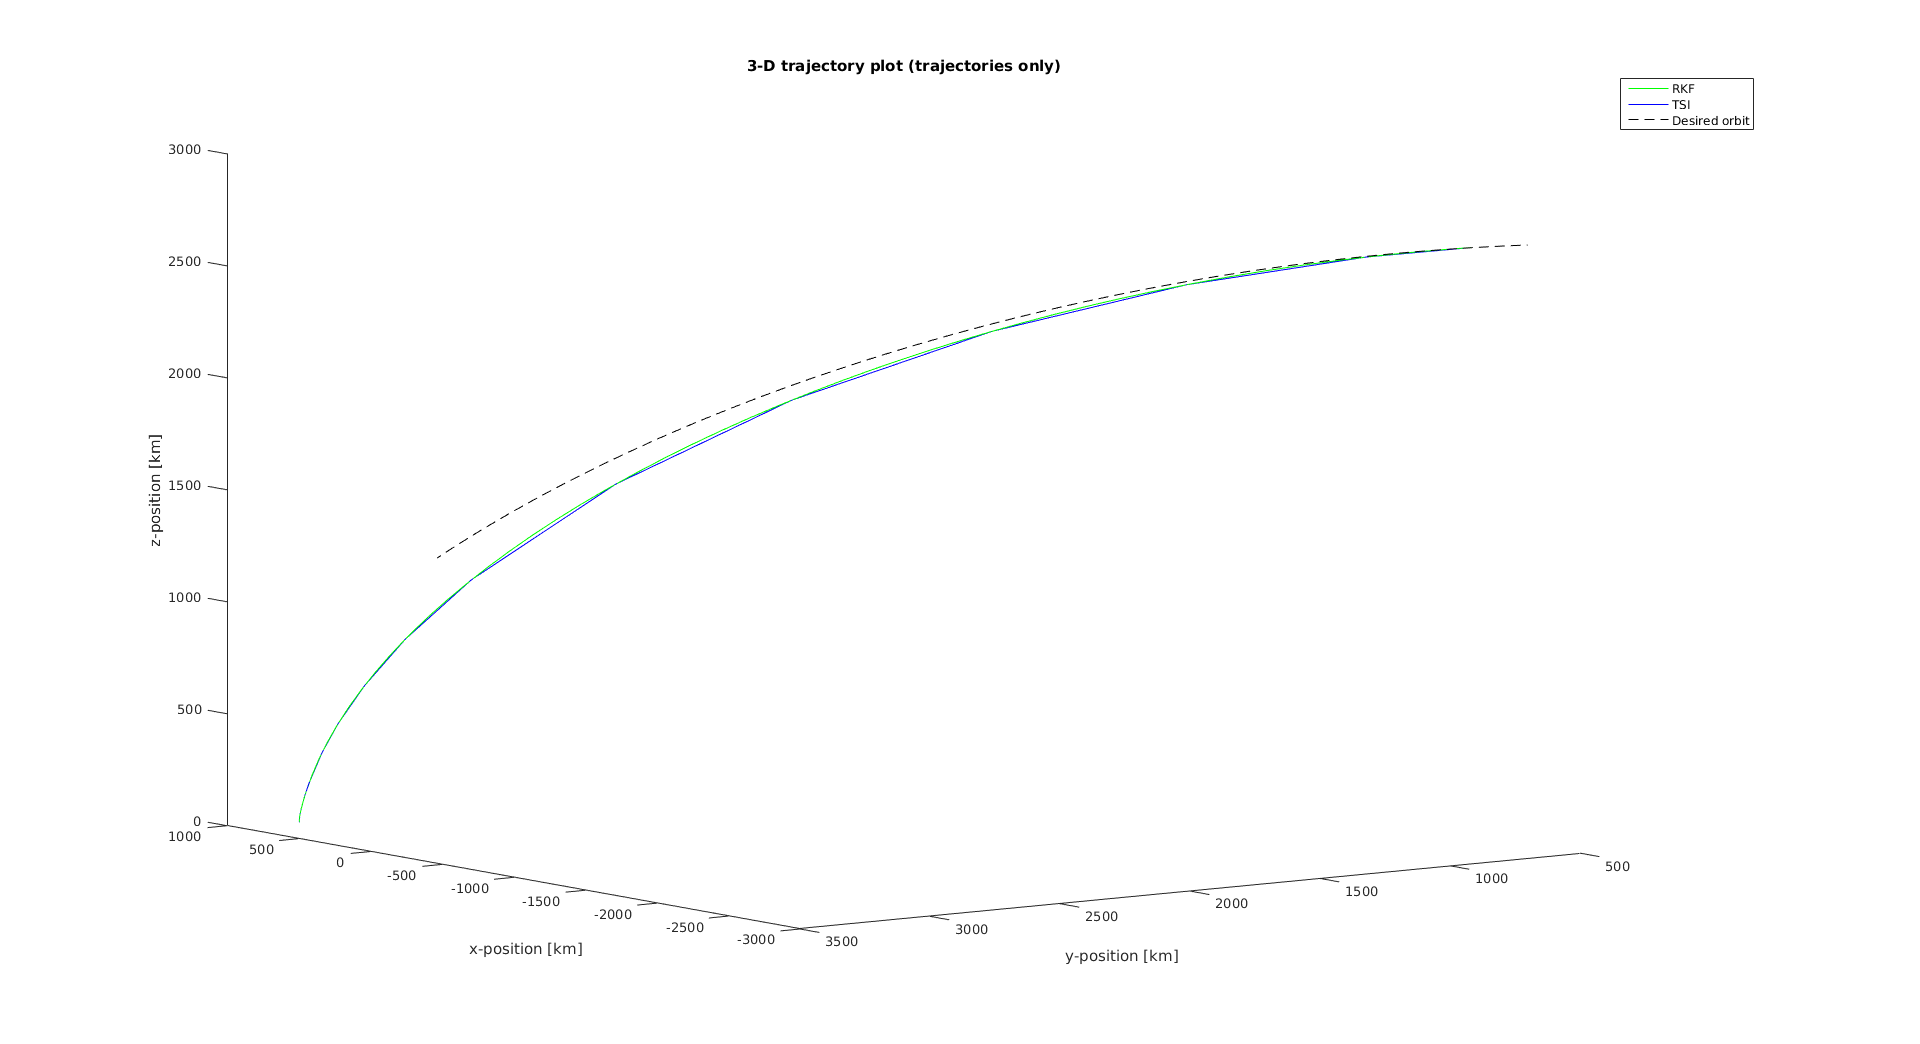
\includegraphics[width=0.8 \textwidth]{figures/verification/case1/PlotFigure2Zoom.png}
\caption{Case 1 3-D trajectory}
\label{fig:PlotFigure2Zoom}
\end{figure}

\begin{figure}[!ht]
\centering
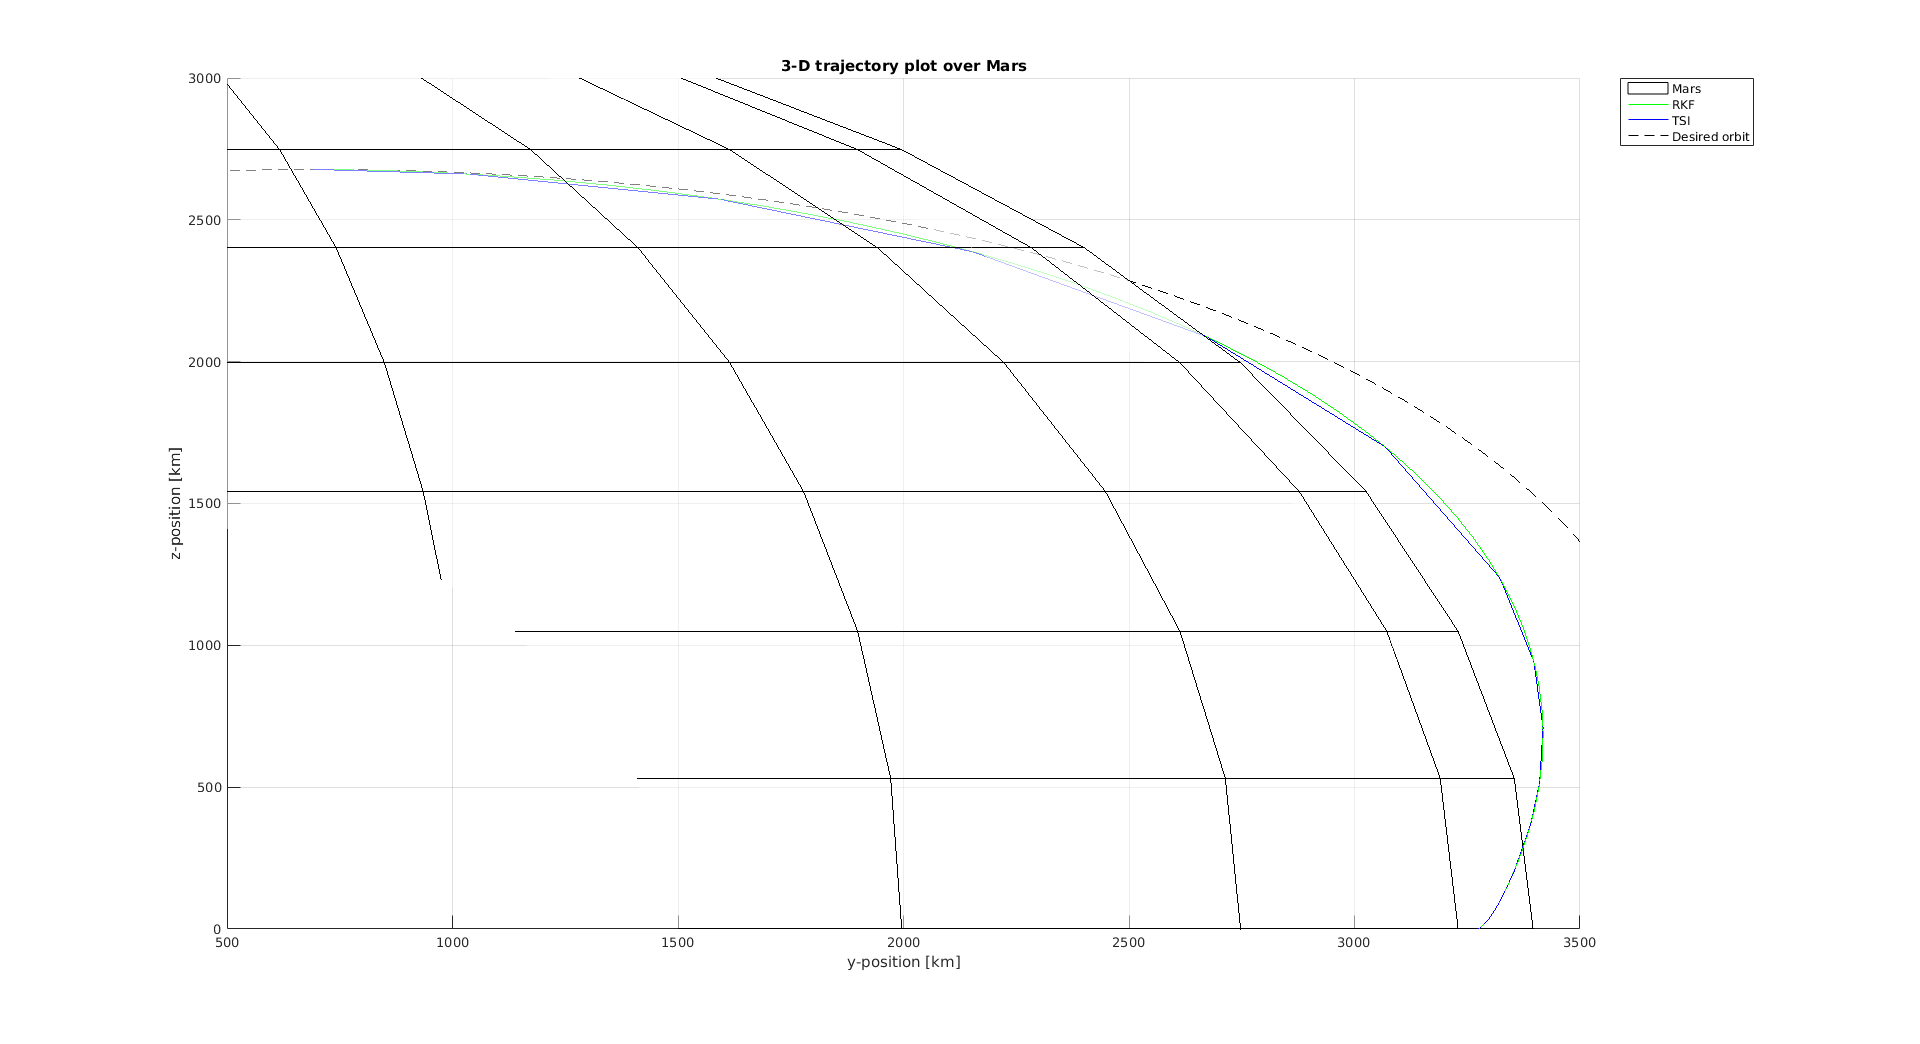
\includegraphics[width=0.8 \textwidth]{figures/verification/case1/PlotFigure1SeenFromZoomXaxis.png}
\caption{Case 1 2-D trajectory as seen from the x-axis}
\label{fig:PlotFigure1SeenFromZoomXaxis}
\end{figure}

\begin{figure}[!ht]
\centering
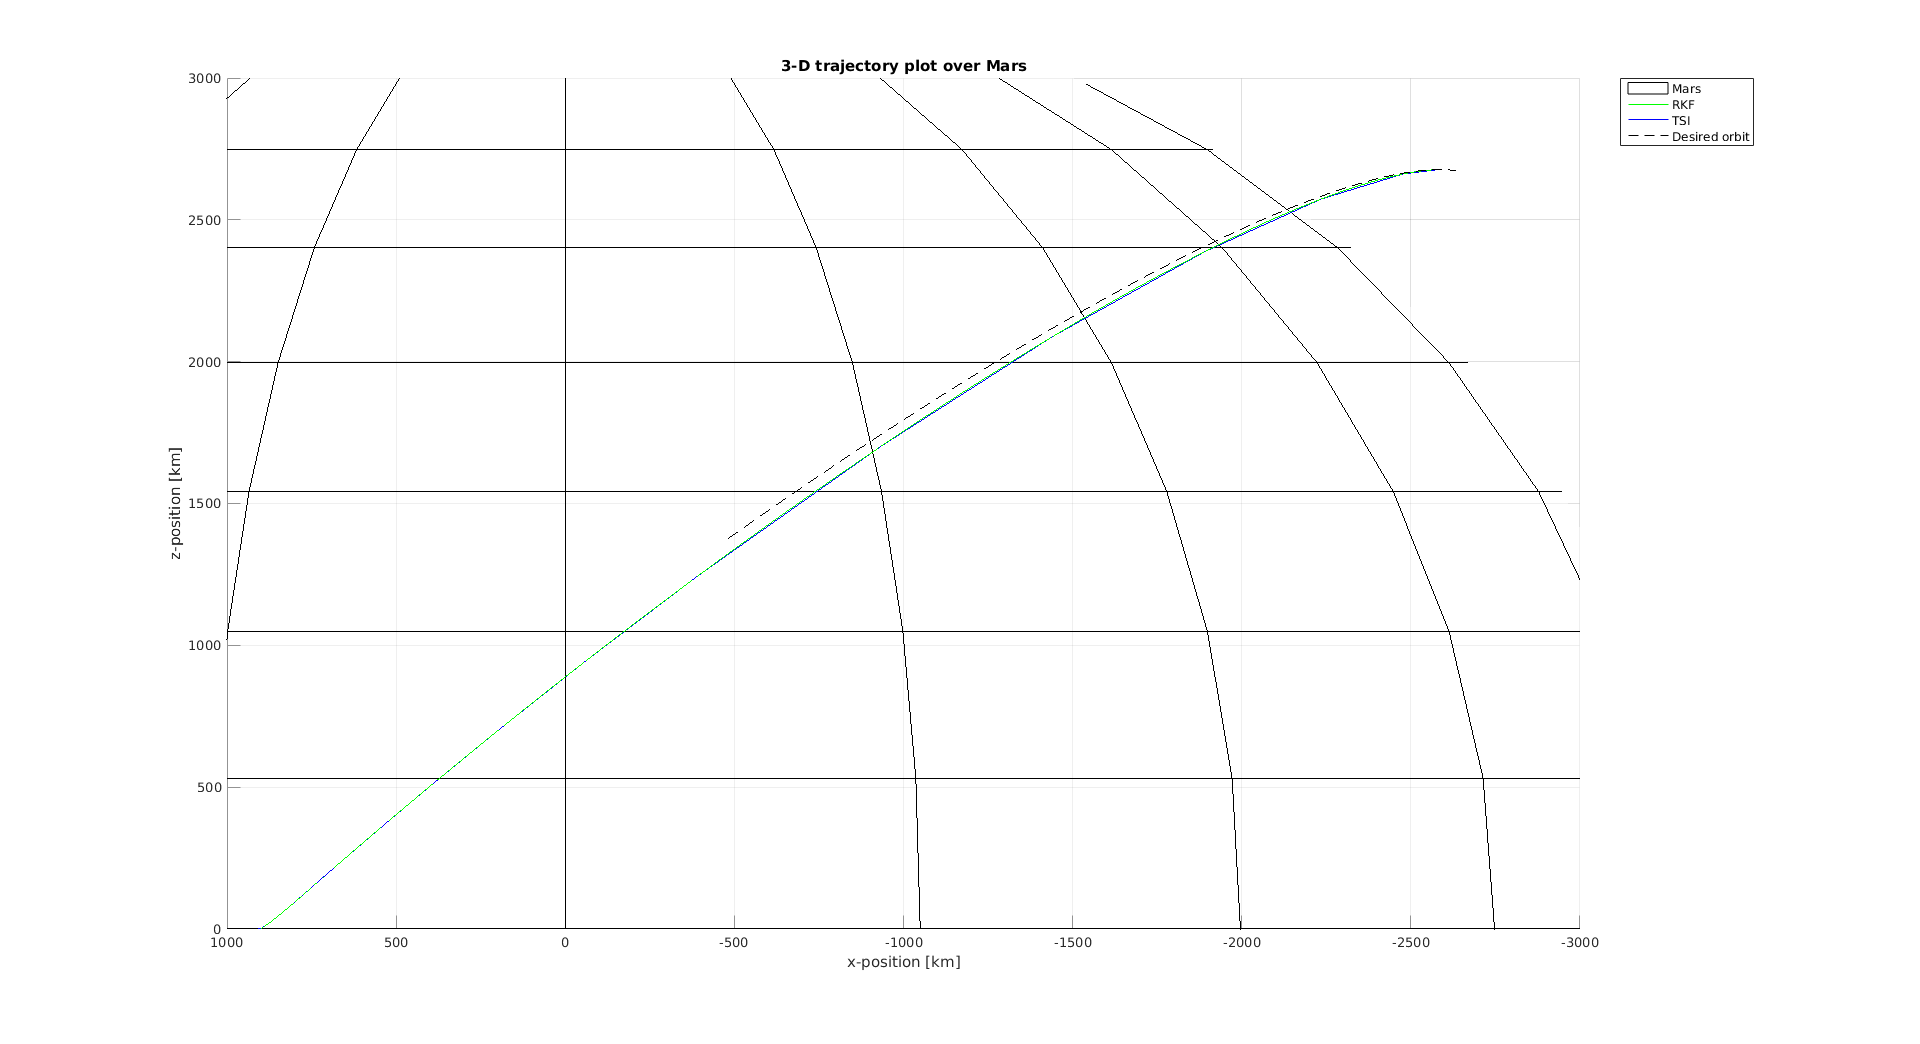
\includegraphics[width=0.8 \textwidth]{figures/verification/case1/PlotFigure1SeenFromZoomYaxis.png}
\caption{Case 1 2-D trajectory as seen from the y-axis}
\label{fig:PlotFigure1SeenFromZoomYaxis}
\end{figure}

\begin{figure}[!ht]
\centering
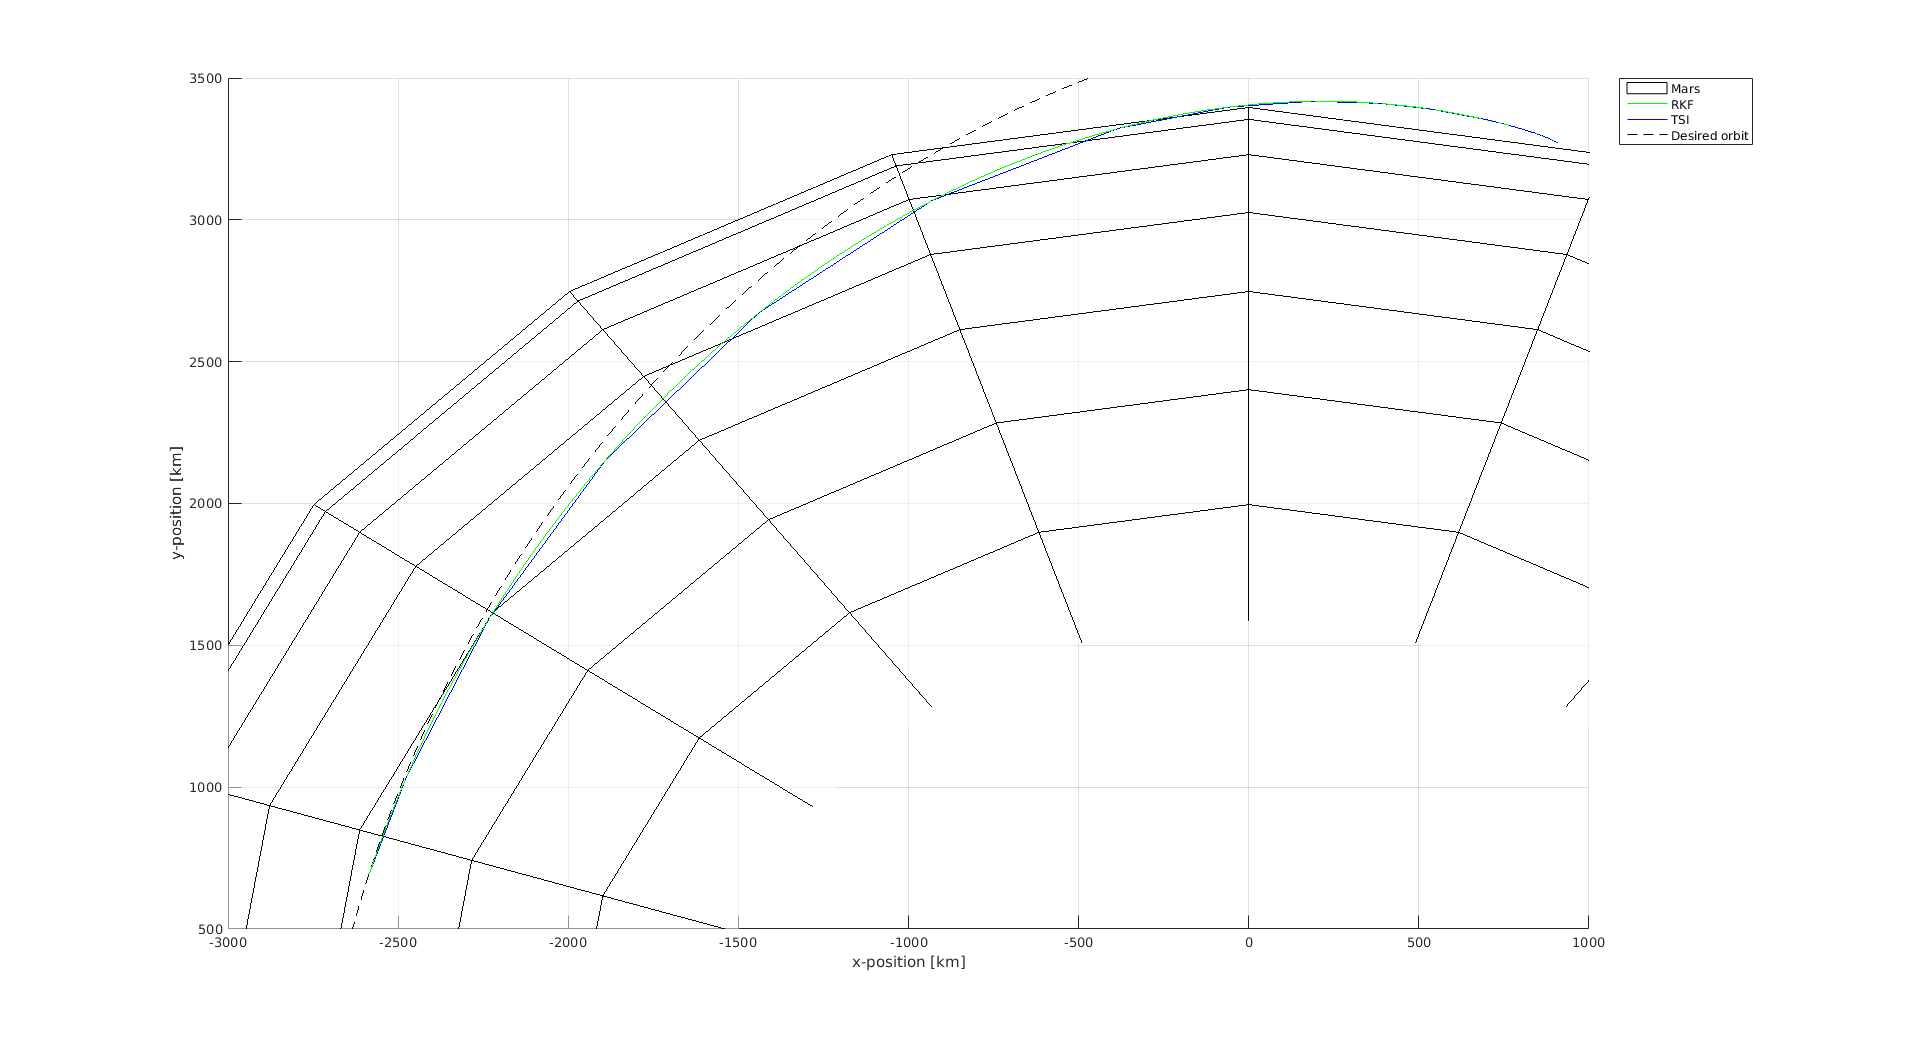
\includegraphics[width=0.8 \textwidth]{figures/verification/case1/PlotFigure1SeenFromZoomZaxis.png}
\caption{Case 1 2-D trajectory as seen from the z-axis}
\label{fig:PlotFigure1SeenFromZoomZaxis}
\end{figure}

A similar validation was done using the second case. However, in this case the reference trajectory was provided. But the main difference here was that the simulation program still was only able to use a constant thrust elevation and azimuth angle. Therefore, the exact profile could not be matched. Benito also included extra perturbing effects creating another difference. However, it was possible to get a trajectory close to the one provided, which is enough for all current purposes. \Cref{tab:validationCaseBenito} shows the used values and computed parameter values for case 2 (similar to case 1).  




\begin{table}[!ht]
\begin{center}
\caption{Validation case 2: \ac{SSTO} Benito}
\label{tab:validationCaseBenito}
\begin{tabular}{|l|l|l||l||l|l|}
\hline 
\textbf{Provided parameters} & \textbf{Given} & \textbf{Used} & \textbf{Provided parameters} & \textbf{Given} & \textbf{Computed} \\ \hline \hline
Thrust [kN] & 6.1087 & 6.0187 & Propellant mass [kg] & 213.85 & 213.85 \\ \hline
I$_{sp}$ [s] & 315.9 & 315.9 & Burn-out angle [deg] & - & 15.644 \\ \hline
Burn Time [s] & 99.362 & 99.362 & Circularisation $\Delta V$ [m/s] & 757.57 & 594.74 \\ \hline
\ac{MAV} \ac{GLOM} [kg] & 288.96 & 288.96 & Ascent time [s] & 949.12 & 876.09 \\ \hline
Launch altitude [km \ac{MOLA}] & -0.8 & -0.6 & Thrust azimuth [deg] & - & -0.7273 \\ \hline
Launch latitude [deg] & 0.0 & 0.0 & Thrust elevation [deg] & - & -0.674 \\ \hline
Launch longitude [deg] & 90 & 90 & & & \\ \hline
Launch ground velocity [km/s] & 1$\cdot $ 10$^{-6}$ & 1$\cdot $ 10$^{-6}$ & & & \\ \hline
Launch \ac{FPA} [deg] & 90 & 89 & & & \\ \hline
Launch Azimuth [deg] & 90 & 90 & & & \\ \hline
Desired altitude [km \ac{MOLA}] & 479.19 & 479.19 & & & \\ \hline
Desired inclination [deg] & 92.69 & 92.69 & & & \\ \hline




\end{tabular}
\end{center}
\end{table}

Again, the trajectory was visualised, however, this time the reference trajectory was also known. In the figures this is represented by a red line. These are shown in \Cref{fig:2PlotFigure2Zoom,fig:2PlotFigure1SeenFromXaxisZoom,fig:2PlotFigure1SeenFromYaxisZoom,fig:2PlotFigure1SeenFromZaxisZoom}.



\begin{figure}[!ht]
\centering
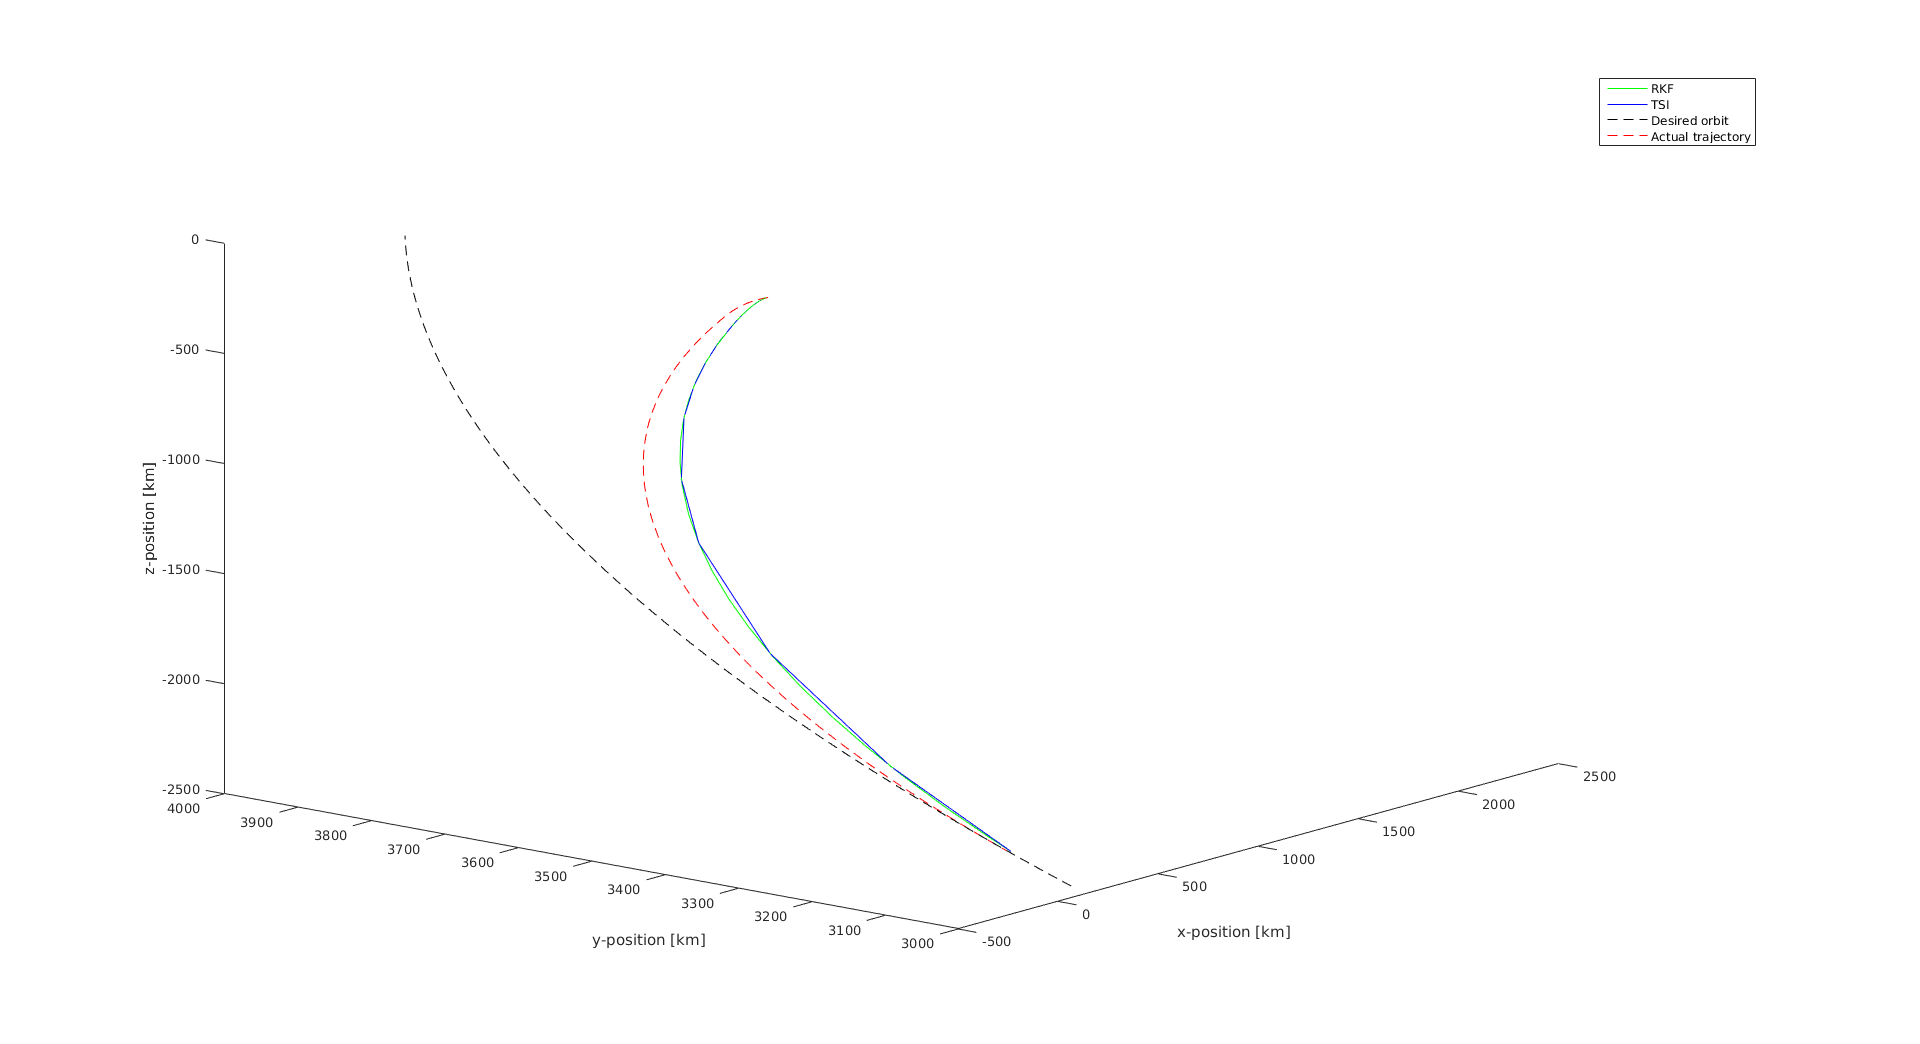
\includegraphics[width=0.8 \textwidth]{figures/verification/case2/PlotFigure2Zoom.png}
\caption{Case 2 3-D trajectory}
\label{fig:2PlotFigure2Zoom}
\end{figure}

\begin{figure}[!ht]
\centering
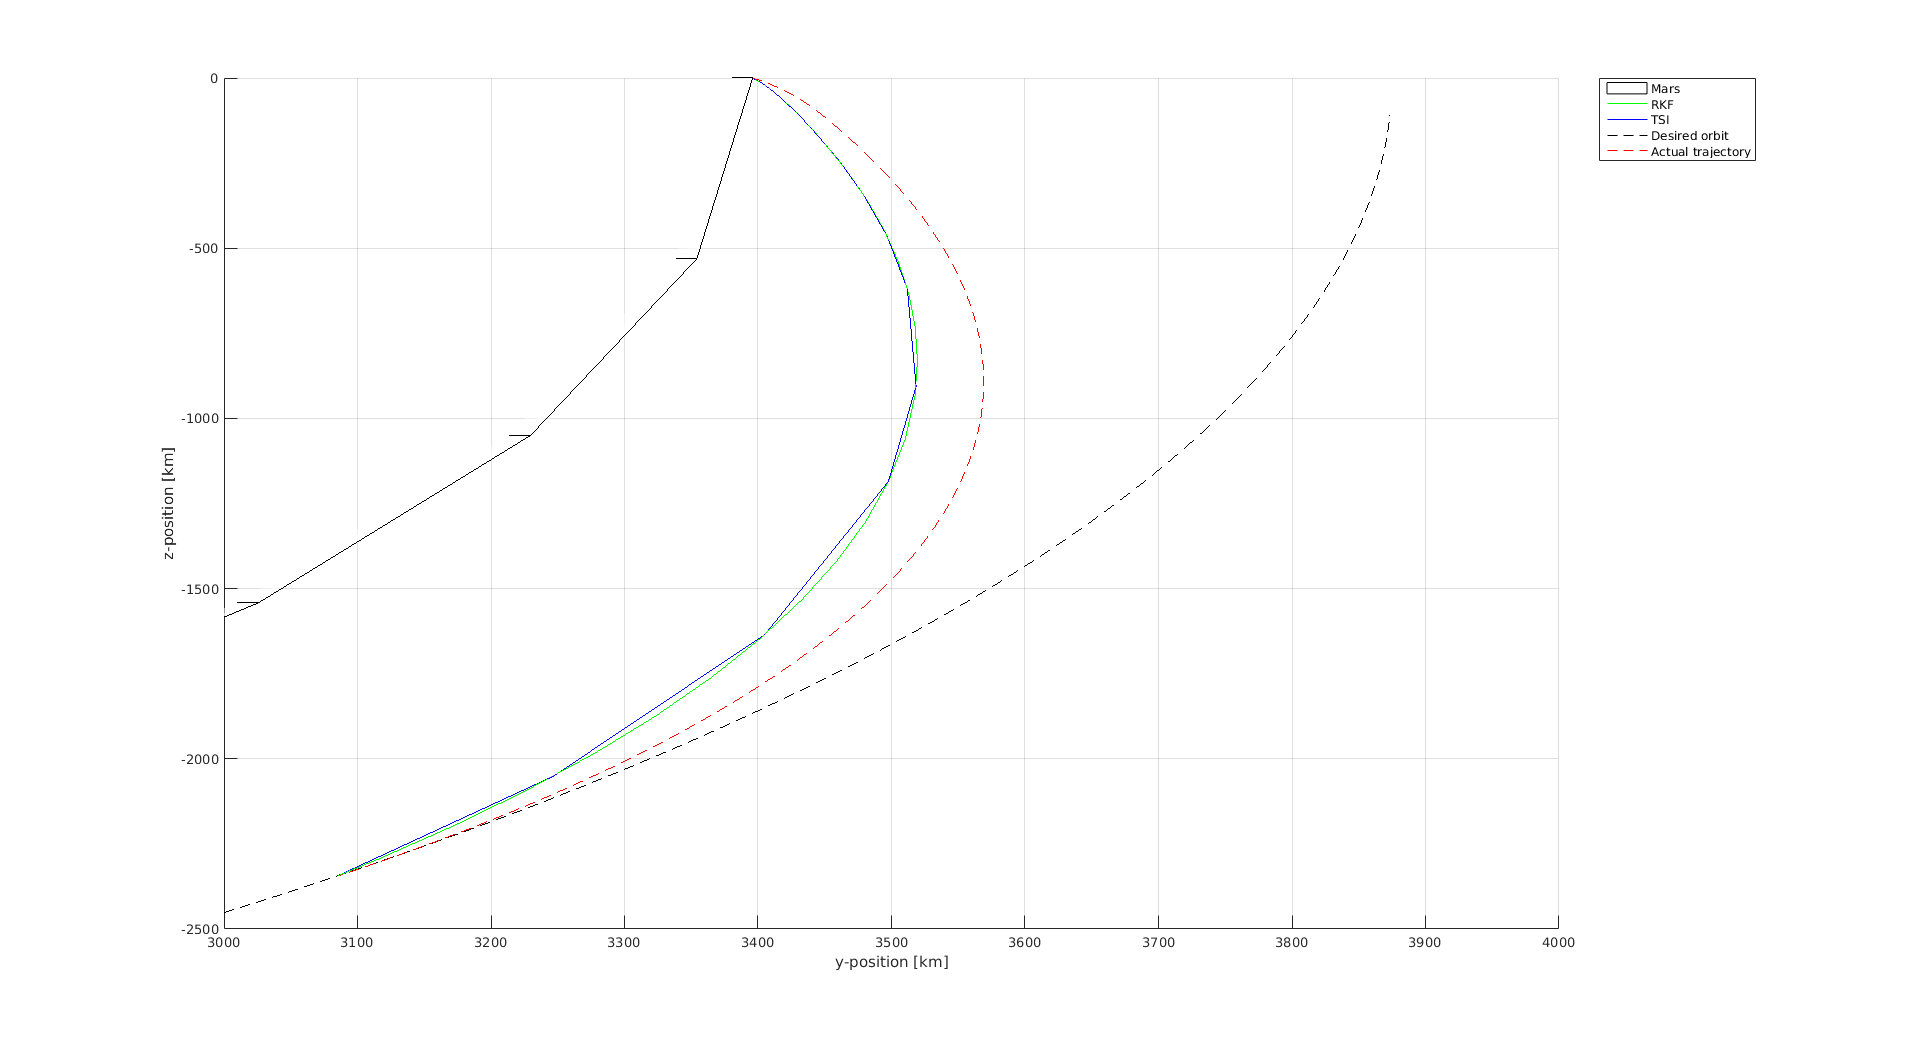
\includegraphics[width=0.8 \textwidth]{figures/verification/case2/PlotFigure1SeenFromXaxisZoom.png}
\caption{Case 2 2-D trajectory as seen from the x-axis}
\label{fig:2PlotFigure1SeenFromXaxisZoom}
\end{figure}

\begin{figure}[!ht]
\centering
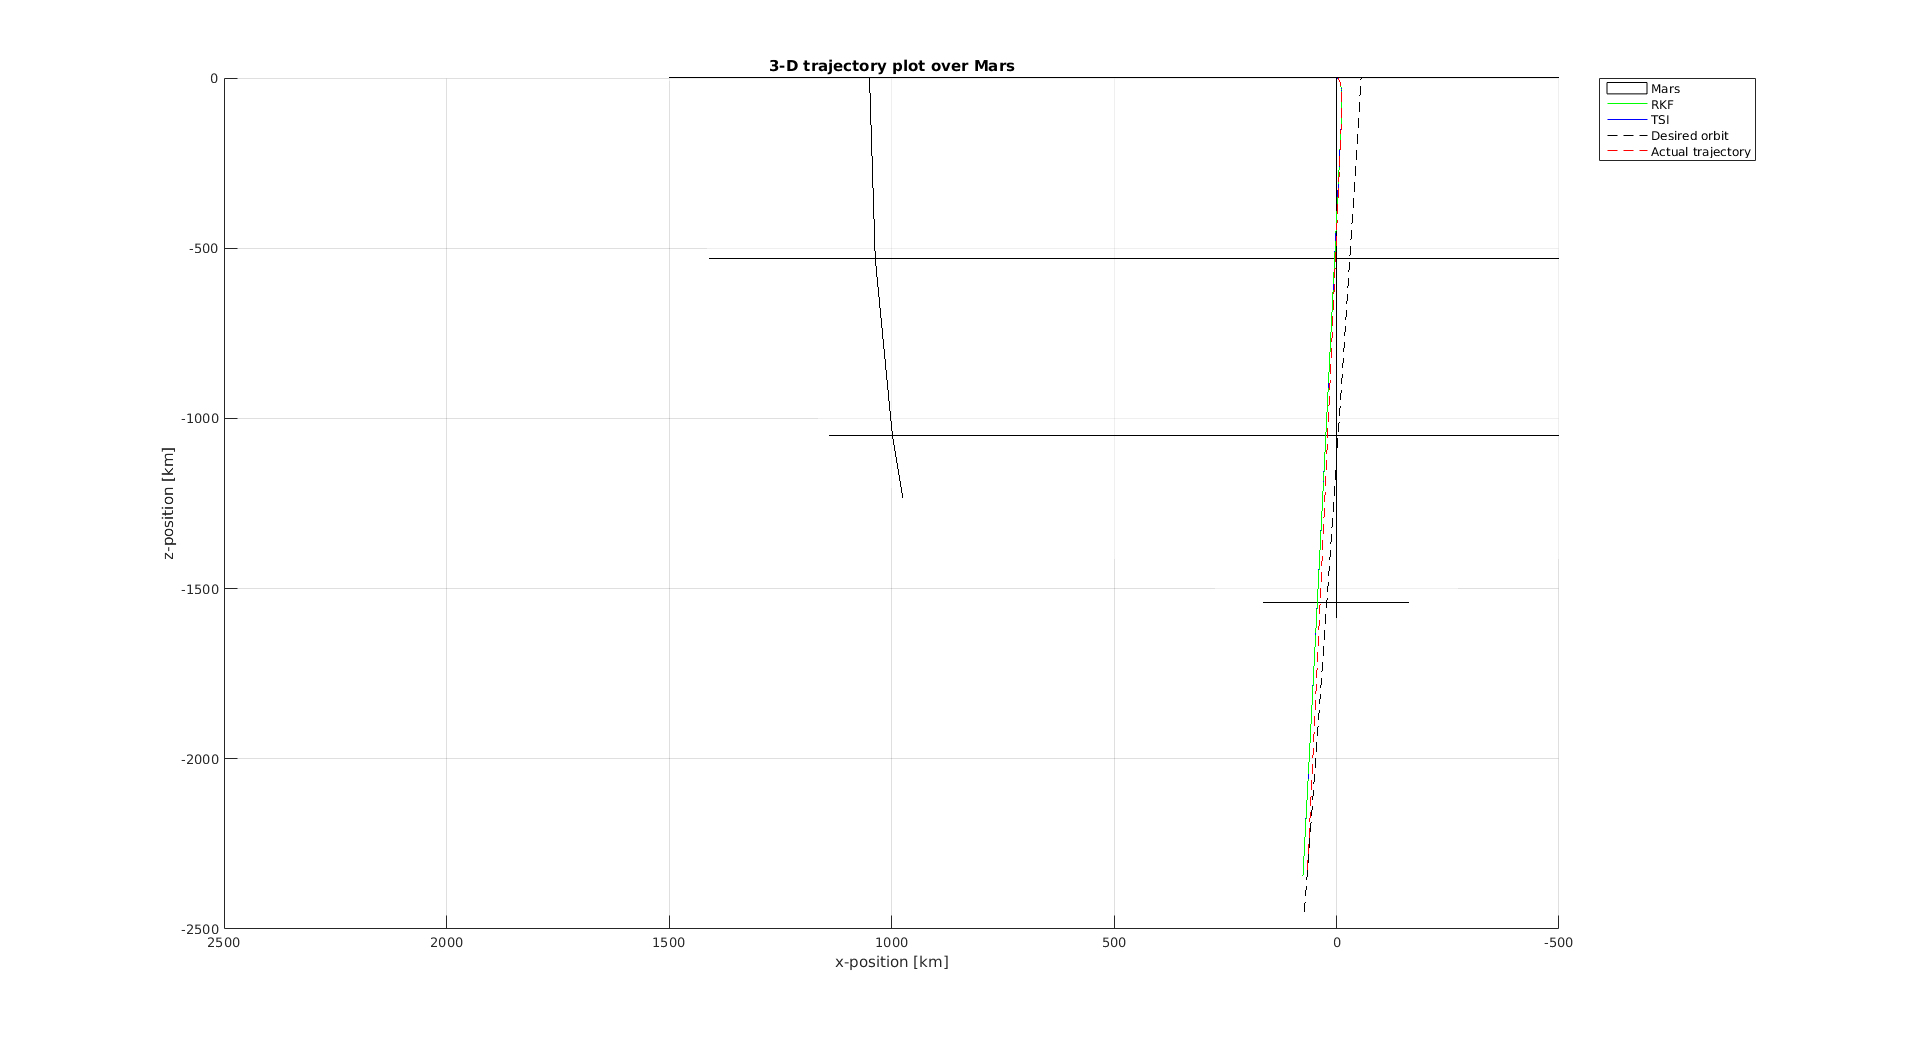
\includegraphics[width=0.8 \textwidth]{figures/verification/case2/PlotFigure1SeenFromYaxisZoom.png}
\caption{Case 2 2-D trajectory as seen from the y-axis}
\label{fig:2PlotFigure1SeenFromYaxisZoom}
\end{figure}

\begin{figure}[!ht]
\centering
\includegraphics[width=0.8 \textwidth]{figures/verification/case2/PlotFigure1SeenFromZaxisZoom.png}
\caption{Case 2 2-D trajectory as seen from the z-axis}
\label{fig:2PlotFigure1SeenFromZaxisZoom}
\end{figure}

The difference in trajectory can mainly be explained by the thrust elevation and thrust azimuth angle curve of the reference trajectory. This curve was derived from the thrust data provided by Benito. This curve is shown in \Cref{fig:thrustAzimuthAndElevationDerivedFromCase2Version2}. 

\begin{figure}[!ht]
\centering
\includegraphics[width=0.8 \textwidth]{figures/verification/case2/thrustAzimuthAndElevationDerivedFromCase2Version2.png}
\caption{Case 2 thrust elevation and azimuth angle curve.}
\label{fig:thrustAzimuthAndElevationDerivedFromCase2Version2}
\end{figure}


%\section{Optimiser}
%\label{sec:optver}
%
%
%\section{Complete optimisation tool}
%\label{sec:opttoolverval}


 % For thesis



\chapter{Results and Analysis} 
%Created 21-12-2016 (04-03-2016 first) 
\label{ch:results}
With the program validated, both case 1 and case 2 can be used to examine the behaviour of \ac{TSI}. This is done in a sensitivity analysis and is very useful to determine the limitations and characteristics of this method. In the previous chapter the trajectories from both \ac{TSI} and \ac{RKF} were plotted and it could be seen that the results were very similar to the point where the accuracy of \ac{TSI} was validated. Therefore, in this chapter the performance of \ac{TSI} will be compared to \ac{RKF} to determine any advantages and disadvantages. In order to do this only one variable will be changed every time, which means that from the nominal case only one parameter will be different. This way the effects can be clearly associated with that particular parameter, which provides a solid base of comparison. The nominal values for both the first and second case are provided in \Cref{app:appendixF-nominalCaseInputValues}. It is also important to have the same cut-off point. This can either be a certain altitude, set end time or zero degrees flight-path angle. Usually the set end time is taken as the cut-off criteria to determine the difference in state. Sometimes the altitude is used in cases where it is interesting to see when a certain altitude is reached and under what conditions when a certain parameter is changed. An example was shown in the validation chapter where certain conditions had to be met at a certain altitude. And in some cases it is best to set the zero degrees flight-path angle as a cut-off criteria because either the cut-off time or altitude will never be reached but the effects of a parameter still need to be investigated. This last cut-off criteria is the "fail-safe" for every simulation because this prevents the simulation from going back to the surface and literally crashing the program. In this chapter every section discusses the effect of a different parameter or focusses on one aspect of the simulation. \\

Besides comparing \ac{TSI} to \ac{RKF} it will also be compared to the non-rotational case. The nominal case takes the rotating Mars into account, however it is interesting to see what \ac{TSI} does when the rotation is turned off. For these two cases to be properly compared, again for most parameters, the set end time is the cut-off criteria unless mentioned otherwise.\\

The parameters changed in this sensitivity analysis are: order, error tolerance, launch altitude, launch latitude, launch longitude, flight-path angle and heading angle. A multiple run analysis will also be described where the nominal case is run for a number of times and the CPU time is compared. 


\section{Order}
\label{sec:order}
For most classic integrators the order is set and cannot be easily changed. For \ac{RKF} for instance, a whole new set of coefficients is required if a different order is desired. However, for \ac{TSI} changing the order is as simple as updating the maximum order input value. Theoretically this means that an infinite order can be chosen to get the most accurate result. The question is, is this indeed the most optimal. \Cref{subsec:optimalOrder} hopes to answer this question by looking at the CPU time. In \Cref{subsec:orderCompNotRot} a range of orders has been run for both cases. Once with the nominal conditions of a rotating Mars and once assuming a non-rotating Mars. The effect of the rotating Mars will be investigated. The cut-off criteria for case 1 was an end time of 1796 seconds for the data collection case and 789 seconds without live data collection. For case 2 the cut-off criteria was 876 second for both runs.

\subsection{Optimal order}
\label{subsec:optimalOrder}
To determine the optimal order an important criteria is that the outcome is accurate, however, what is often more important is that this accurate outcome is computed really fast. This is why, in order to find the optimum order, the CPU time is the most important criteria. In order to properly observe the effect of a different order, the nominal case is run for different orders. Thus the only difference will be the maximum order. This can be done for the two presented cases. During real-life simulations a user can choose to either collect all the data during the simulation or only store the final outcomes at the end of the simulation. Storing data during the integration requires a lot of computational power and will therefore increase the CPU time required, but this will provide the user with the desired trajectory data. Both cases with and without live data collection have been run for a specific range of orders depending on the case, and the results are shown in \Cref{fig:orderVsCPUcase1IncludingLiveDataCollection}.
The first case was run with a maximum order ranging from 5 to 100, and the second case was run from 5 to 31 because of the behaviour observed during the first case runs. 



\begin{figure}[H]
\centering
\subfloat[]{\includegraphics[width=3.1in]{figures/results/Order/orderVsCPUcase1IncludingLiveDataCollection.png}\label{subfig:orderVsCPUcase1IncludingLiveDataCollection}} 
\subfloat[]{\includegraphics[width=3.1in]{figures/results/Order/orderVsCPUcase2IncludingLiveDataCollection.png} \label{subfig:orderVsCPUcase2IncludingLiveDataCollection}}\\
 
\subfloat[]{\includegraphics[width=3.1in]{figures/results/Order/orderVsCPUcase1NoDataCollection.png}\label{subfig:orderVsCPUcase1NoDataCollection}} 
\subfloat[]{\includegraphics[width=3.1in]{figures/results/Order/orderVsCPUcase2NoDataCollection.png}\label{subfig:orderVsCPUcase2NoDataCollection}}
\caption{Order versus CPU time \protect\subref{subfig:orderVsCPUcase1IncludingLiveDataCollection} case 1 including live data collection, \protect\subref{subfig:orderVsCPUcase2IncludingLiveDataCollection} case 2 including live data collection, \protect\subref{subfig:orderVsCPUcase1NoDataCollection} case 1 without live data collection, \protect\subref{subfig:orderVsCPUcase2NoDataCollection} case 2 without live data collection } 
\label{fig:orderVsCPUcase1IncludingLiveDataCollection} 
\end{figure} 

Looking at \Cref{subfig:orderVsCPUcase1IncludingLiveDataCollection} it is clear that the order versus CPU curve can be split up into two phases that have different properties that influence the CPU time. The first phase shows a rapid decrease in the CPU time until order 20 is reached, the second phase continues from that point until the final order is reached. The order has a direct relation to the chosen step-size that \ac{TSI} computes automatically because the step-size is determined by the error tolerance and the difference between the penultimate Taylor Series coefficient and the final one (as described in \Cref{subsec:stepSizeTsi}). This means that if these last two coefficients show a large difference, which can happen lower order because fewer derivatives are taken into account, the step-size will be lowered and thus increasing the number of steps. In the first phase, this large number of steps result in a high CPU time. Another factor that affects the CPU time is the number of derivatives taken into account, which is directly related to the order (10 as maximum order equals 10 derivatives that are taken into account). At a certain point, an increase in order does not affect the number of steps that much any more, resulting in a decrease of 3 to 1 steps with every order increase. The result is that the number of steps remains approximately the same but the number of derivatives that are taken into account keeps increasing. Every extra derivative means an extra computation per auxiliary equation/variable. This is what is observed in the second phase. Here the effect of adding more computations on the CPU time becomes clear, showing a corresponding increase in CPU time. This tipping point between the two phases can be observed around the lowest CPU time, where the effect of the number of steps and the number of derivative computations equal out. This is therefore the optimum order for the \ac{TSI} method. The two phases can be observed in each of the four graphs, however, because the increase of CPU time, the higher orders were not required and were thus left out in the simulations for case 2. For each of the simulation runs, the two orders which resulted in the lowest CPU time have been recorded in \Cref{tab:orderAndCPUtimes}. 

\begin{table}[H]
\begin{center}
\caption{Lowest two orders with corresponding CPU times for each of the sub-graphs}
\label{tab:orderAndCPUtimes}
\begin{tabular}{|l|l|l|l|l|}
\hline 
\textbf{Sub-graph}  & \multicolumn{2}{c|}{\textbf{Lowest CPU time}} & \multicolumn{2}{c|}{\textbf{Second lowest CPU time}} \\ \cline{2-5}

& \textbf{Order} &
\textbf{CPU time [s]} & \textbf{Order} & \textbf{CPU time [s]} \\ \hline \hline

a & 20 & 0.053162 & 21 & 0.053226 \\ \hline
b & 25 & 0.083474 & 22 & 0.0837 \\ \hline
c & 14 & 0.007465 & 20 & 0.007736 \\ \hline
d & 18 & 0.008273 & 20 & 0.008314 \\ \hline


\end{tabular}
\end{center}
\end{table}

In the table and the graphs it can be seen that the minima are all situated around an order of 20, which is why a maximum order of 20 was set as the nominal value and used for all simulations.

%a: 20 = 0.053162 s, 21 = 0.053226 s
%b: 25 = 0.083474 s, 22 = 0.0837 s
%c: 14 = 0.007465 s, 20 = 0.007736 s
%d: 18 = 0.008273 s, 20 = 0.008314 s

%Show both plots of orders and then talk about the fastest order and explain what you can see. First part of graph is the number of evaluations important and last part is the amount of computations that have to be made because the number of evaluations don't change any more.
%
%Graphs needed:
%
%- CPU time vs order case 1 and case 2


% \begin{figure}[H]
%\centering
%\includegraphics[width=0.7\textwidth]{figures/results/Order/orderVsCPUcase1IncludingLiveDataCollection.png}
%\caption{Order versus CPU time case 1 including live data collection.}
%\label{fig:orderVsCPUcase1IncludingLiveDataCollection}
%\end{figure}

%\begin{figure}
%\centering
%\subfloat[]{\includegraphics[width=3.1in]{figures/results/Order/orderVsCPUcase1IncludingLiveDataCollection.png}\label{subfig:orderVsCPUcase1IncludingLiveDataCollection}} 
%\subfloat[]{\includegraphics[width=3.1in]{figures/results/Order/orderVsCPUcase2IncludingLiveDataCollection.png}\label{subfig:orderVsCPUcase2IncludingLiveDataCollection}}
%\caption{Order versus CPU time including live data collection \protect\subref{subfig:orderVsCPUcase1IncludingLiveDataCollection} case 1 \protect\subref{subfig:orderVsCPUcase2IncludingLiveDataCollection} case 2 } 
%\label{fig:orderVsCPUcase1IncludingLiveDataCollection} 
%\end{figure} 
%
%\begin{figure}
%\centering
%\subfloat[]{\includegraphics[width=3.1in]{figures/results/Order/orderVsCPUcase1NoDataCollection.png}\label{subfig:orderVsCPUcase1NoDataCollection}} 
%\subfloat[]{\includegraphics[width=3.1in]{figures/results/Order/orderVsCPUcase2NoDataCollection.png}\label{subfig:orderVsCPUcase2NoDataCollection}}
%\caption{Order versus CPU time without live data collection \protect\subref{subfig:orderVsCPUcase1NoDataCollection} case 1 \protect\subref{subfig:orderVsCPUcase2NoDataCollection} case 2 } 
%\label{fig:orderVsCPUcase1NoDataCollection} 
%\end{figure} 

%Tables needed:
%
%- Zoom in numbers around Order 20 to prove it is the fastest \\

\subsection{Comparison with non-rotating Mars}
\label{subsec:orderCompNotRot}
For the comparison of the rotating and the non-rotating cases with a varying order it is again interesting to look at the differences in CPU time. \Cref{fig:orderVsCPUcase1combined} shows these plots for both cases when the trajectory data is not collected during the simulation. It can be seen that for case 1, on average, the non-rotating runs are faster. Also, for a non-rotating Mars the optimum order is 20 as well. The difference in CPU time is better shown by the case 2 run, where the non-rotating curve fits perfectly below the rotating curve. Here, the order 20 has again the second lowest CPU time (the lowest is order 17 with a time difference of 28 microseconds). The time difference between the curves of the rotating and non-rotating Mars can be explained by the fact that if Mars does not rotate, the rotating effects become zero, which reduces the number of computations.
%Explain what you can see in the graph and why that is probably the case.
%
%Graphs needed:
%
%- CPU time vs order case 1 combined \\
%- CPU time vs order case 2 combined \\
%
%
%- RKF difference in end state before circularisation combined case 1 \\ 
%- RKF difference in end state before circularisation combined case 2 \\
%- Consecutive difference in end state before cicularisation combined case 1 \\
%- Consecutive difference in end state before cicularisation combined case 2 \\
%- Nominal case difference in end state before circularisation combined case 1 \\
%- Nominal case difference in end state before circularisation combined case 2 \\
%


\begin{figure}[H]
\centering
\subfloat[]{\includegraphics[width=3.1in]{figures/results/Order/orderVsCPUcase1combined.png}\label{subfig:orderVsCPUcase1combined}} 
\subfloat[]{\includegraphics[width=3.1in]{figures/results/Order/orderVsCPUcase2combined.png}\label{subfig:orderVsCPUcase2combined}}
\caption{Order versus CPU time for rotating and non-rotating Mars \protect\subref{subfig:orderVsCPUcase1combined} case 1,  \protect\subref{subfig:orderVsCPUcase2combined} case 2 } 
\label{fig:orderVsCPUcase1combined} 
\end{figure} 

As was mentioned before, the accuracy of  the results is very important. In \Cref{fig:orderVsRKFAbsoluteDifferenceCase1combined} the absolute difference between the nominal end state of \ac{RKF} before circularisation and \ac{TSI} for both the rotating and non-rotating Mars. A trend can be identified where it is shown that an order of 11 or higher will result in a difference of $\mu$m in position and nm/s in velocity. Even the lowest order of 5 results in an accuracy of less than 10 cm for position and 10 mm/s for velocity. The spikes in the first case are caused by a slight error resulting from the combination of variables that result at those specific orders. This proves that the simulator is not yet robust enough and could still use some improvements. One improvement that might solve this problem is a change in the manner in which the step-size is computed. Additional comparison plots are shown in \Cref{app:appendixG-Results}.

\begin{figure}[H]
\centering
\subfloat[]{\includegraphics[width=1.1\textwidth]{figures/results/Order/orderVsRKFAbsoluteDifferenceCase1combined.png}\label{subfig:orderVsRKFAbsoluteDifferenceCase1combined}}\\
 
 
\subfloat[]{\includegraphics[width=1.1\textwidth]{figures/results/Order/orderVsRKFAbsoluteDifferenceCase2combined.png}\label{subfig:orderVsRKFAbsoluteDifferenceCase2combined}}
\caption{Difference with respect to \ac{RKF} case for rotating and non-rotating Mars \protect\subref{subfig:orderVsRKFAbsoluteDifferenceCase1combined} case 1,  \protect\subref{subfig:orderVsRKFAbsoluteDifferenceCase2combined} case 2 } 
\label{fig:orderVsRKFAbsoluteDifferenceCase1combined} 
\end{figure}


\section{Error tolerance}
\label{sec:errorTolerance}
The error tolerance is used to determine the required step-size during the integration. A high error tolerance (say 10$^{-5}$) will therefore provide an end result that is less accurate than a lower error tolerance (such as 10$^{-15}$). For the \ac{RKF78} provided by \ac{Tudat} the lowest accuracy that can be used is 10$^{-15}$, which is why that accuracy is used as the nominal accuracy. When a range of error tolerances is examined the accuracy of the end state and the speed of convergence can be determined. The speed of convergence follows from the consecutive differences between the end states and the accuracy of the end states comes from the comparison to the nominal case. Both these characteristics will be examined and compared for \ac{RKF} and \ac{TSI}, see \Cref{subsec:errorToleranceCompRKF}, and for the rotating and non-rotating Mars described in \Cref{subsec:errorToleranceCompNotRot}. The cut-off criteria for case 1 was 789 seconds and 876 seconds for case 2 and both cases were run without live data collection.


%Mention what I want to discuss in this section.


\subsection{Comparison with \ac{RKF78}}
\label{subsec:errorToleranceCompRKF}
The speed of convergence is important because it shows the relationship between the different error tolerances. If the differences are small it means that the change in error tolerance had a small effect. If the consecutive difference is large, it means that the solution has not yet converged. \Cref{fig:errorToleranceVsConsecutiveDifferenceCase1RKFTSIpositionSmall} shows the consecutive differences in position and velocity for the two cases for both integration methods. Here it can clearly be seen that \ac{TSI} converges much faster than \ac{RKF}. The curve of \ac{RKF} lies quite a bit higher, which means that the differences are larger, and thus it converges slower than \ac{TSI}.


%Show the faster convergence of end state before circularisation.


%Graphs needed:
%
%- Consecutive difference graphs RKF and TSI combined for case 1 \\
%- Consecutive difference graphs RKF and TSI combined for case 2 \\
%- Nominal case difference in end state before circularisation RKF and TSI combined case 1 \\
%- Nominal case difference in end state before circularisation RKF and TSI combined case 2 \\

\begin{figure}[H]
\centering
\subfloat[]{\includegraphics[width=3.1in]{figures/results/errorTolerance/errorToleranceVsConsecutiveDifferenceCase1RKFTSIpositionSmall.png}\label{subfig:errorToleranceVsConsecutiveDifferenceCase1RKFTSIpositionSmall}} 
\subfloat[]{\includegraphics[width=3.1in]{figures/results/errorTolerance/errorToleranceVsConsecutiveDifferenceCase2RKFTSIpositionSmall.png} \label{subfig:errorToleranceVsConsecutiveDifferenceCase2RKFTSIpositionSmall}}\\
 
\subfloat[]{\includegraphics[width=3.1in]{figures/results/errorTolerance/errorToleranceVsConsecutiveDifferenceCase1RKFTSIvelocitySmall.png}\label{subfig:errorToleranceVsConsecutiveDifferenceCase1RKFTSIvelocitySmall}} 
\subfloat[]{\includegraphics[width=3.1in]{figures/results/errorTolerance/errorToleranceVsConsecutiveDifferenceCase2RKFTSIvelocitySmall.png}\label{subfig:errorToleranceVsConsecutiveDifferenceCase2RKFTSIvelocitySmall}}
\caption{Error tolerance versus consecutive difference between end states before circularisation for \ac{TSI} and \ac{RKF} \protect\subref{subfig:errorToleranceVsConsecutiveDifferenceCase1RKFTSIpositionSmall} case 1 position, \protect\subref{subfig:errorToleranceVsConsecutiveDifferenceCase2RKFTSIpositionSmall} case 2 position, \protect\subref{subfig:errorToleranceVsConsecutiveDifferenceCase1RKFTSIvelocitySmall} case 1 velocity, \protect\subref{subfig:errorToleranceVsConsecutiveDifferenceCase2RKFTSIvelocitySmall} case 2 velocity } 
\label{fig:errorToleranceVsConsecutiveDifferenceCase1RKFTSIpositionSmall} 
\end{figure} 

A similar comparison can be done when comparing each of the end states directly to the nominal end state. The result is a nominal absolute difference graph as presented in \Cref{fig:errorToleranceVsNominalAbsoluteDifferenceCase1RKFTSIpositionSmall} for position and velocity and both cases. Here it can be seen that the accuracy of the position at an error tolerance of 10$^{-5}$ is already in cm for \ac{TSI} whereas this accuracy is only reached at an error tolerance of 10$^{-9}$ for \ac{RKF}. For the velocity the \ac{TSI} accuracy is in the order of 10 $\mu$m at this initial error tolerance which also is reached at an error tolerance of 10$^{-9}$ using \ac{TSI}. This means that \ac{TSI} is, on average, more accurate at any given error tolerance.  

\begin{figure}[H]
\centering
\subfloat[]{\includegraphics[width=3.1in]{figures/results/errorTolerance/errorToleranceVsNominalAbsoluteDifferenceCase1RKFTSIpositionSmall.png}\label{subfig:errorToleranceVsNominalAbsoluteDifferenceCase1RKFTSIpositionSmall}} 
\subfloat[]{\includegraphics[width=3.1in]{figures/results/errorTolerance/errorToleranceVsNominalAbsoluteDifferenceCase2RKFTSIpositionSmall.png} \label{subfig:errorToleranceVsNominalAbsoluteDifferenceCase2RKFTSIpositionSmall}}\\
 
\subfloat[]{\includegraphics[width=3.1in]{figures/results/errorTolerance/errorToleranceVsNominalAbsoluteDifferenceCase1RKFTSIvelocitySmall.png}\label{subfig:errorToleranceVsNominalAbsoluteDifferenceCase1RKFTSIvelocitySmall}} 
\subfloat[]{\includegraphics[width=3.1in]{figures/results/errorTolerance/errorToleranceVsNominalAbsoluteDifferenceCase2RKFTSIvelocitySmall.png}\label{subfig:errorToleranceVsNominalAbsoluteDifferenceCase2RKFTSIvelocitySmall}}
\caption{Error tolerance versus nominal absolute difference between end states before circularisation for \ac{TSI} and \ac{RKF} \protect\subref{subfig:errorToleranceVsNominalAbsoluteDifferenceCase1RKFTSIpositionSmall} case 1 position, \protect\subref{subfig:errorToleranceVsNominalAbsoluteDifferenceCase2RKFTSIpositionSmall} case 2 position, \protect\subref{subfig:errorToleranceVsNominalAbsoluteDifferenceCase1RKFTSIvelocitySmall} case 1 velocity, \protect\subref{subfig:errorToleranceVsNominalAbsoluteDifferenceCase2RKFTSIvelocitySmall} case 2 velocity } 
\label{fig:errorToleranceVsNominalAbsoluteDifferenceCase1RKFTSIpositionSmall} 
\end{figure} 

Another important observation can be made when looking at the difference in function evaluations and CPU time for each error tolerance for both \ac{RKF} and \ac{TSI}. The values for both cases are shown in \Cref{tab:RKFvsTSIfunctionEvaluationAndCPUtime}.



\begin{table}[H]
\begin{center}
\caption{Number of function evaluations and CPU time for \ac{RKF} and \ac{TSI}}
\label{tab:RKFvsTSIfunctionEvaluationAndCPUtime}
\begin{tabular}{|l|p{1.5cm}|p{1.5cm}|l|l|p{1.5cm}|p{1.5cm}|l|l|}
\hline 
\textbf{Error}  & \multicolumn{4}{c|}{\textbf{Case 1}} & \multicolumn{4}{c|}{\textbf{Case 2}} \\ \cline{2-9}

\textbf{tolerance} & \multicolumn{2}{c|}{Number of evaluations} & \multicolumn{2}{c|}{CPU time [ms]}& \multicolumn{2}{c|}{Number of evaluations} & \multicolumn{2}{c|}{CPU time [ms]} \\ \cline{2-9}

& \textbf{\ac{RKF}} &
\textbf{\ac{TSI}} & \textbf{\ac{RKF}} & \textbf{\ac{TSI}} & \textbf{\ac{RKF}} &
\textbf{\ac{TSI}} & \textbf{\ac{RKF}} & \textbf{\ac{TSI}} \\ \hline \hline

10$^{-5}$ & 169 & 24 & 0.419 &4.703 &156 &24 &0.392 &5.353 \\ \hline
10$^{-6}$ & 182 & 24 & 0.432 &4.57 &182 &25 &0.49 &5.518 \\ \hline
10$^{-7}$ & 221 & 26 & 0.542 &4.769 &208 &27 &0.527 &5.823 \\ \hline
10$^{-8}$ & 260 & 29 & 0.614 &5.272 &247 &29 &0.567 &6.354 \\ \hline
10$^{-9}$ & 312 & 30 & 0.823 &5.571 &286 &30 &0.709 &6.439 \\ \hline
10$^{-10}$ & 364 & 32 & 0.845 &5.685 &338 &33 &0.789 &7.083 \\ \hline
10$^{-11}$ & 455 & 36 & 1.032 &6.227 &390 &36 &0.904 &7.454 \\ \hline
10$^{-12}$ & 546 & 38 & 1.277 &6.506 &546 &39 &1.231 &8.02 \\ \hline
10$^{-13}$ & 702 & 41 & 1.541 &7.062 &728 &41 &1.604 &8.627 \\ \hline
10$^{-14}$ & 910 & 42 & 1.965 &7.227 &936 &45 &2.055 &9.538 \\ \hline
10$^{-15}$ & 1222 & 46 & 2.666 &7.754 &1300 &47 &2.851 &9.538 \\ \hline


\end{tabular}
\end{center}
\end{table}

Here one evaluation is defined as running through the derivative equations once. For \ac{TSI} this means that each time step, one evaluation is performed because all desired derivatives are computed during one computational run. In the case of \ac{RKF78} however, each time step consists of 13 computational runs. \Cref{tab:RKFvsTSIfunctionEvaluationAndCPUtime} shows that for both cases the number of evaluations of \ac{RKF} are approximately one order more at the high error tolerances but almost two orders higher at the lowest tolerance compared to \ac{TSI}. This means that a decrease in error tolerance results in a large increase in number of evaluations for \ac{RKF} but a relatively small increase for \ac{TSI}. For both cases, the number of evaluations is not even doubled from the highest to the lowest tolerance, whereas the maximum number of evaluations for \ac{RKF} is 7 to 8 times more. \\

This advantage however does not translate well to the CPU time where it can be seen that for most of the error tolerances \ac{RKF} is an order faster than \ac{TSI}. The similar increase in CPU time for both integrators is nevertheless still observed. An explanation for the large difference in CPU time could be that \ac{TSI} was not optimally programmed and thus results in a relatively high CPU time. Further analysis is required.

%Compare the number of function evaluations and explain why you should look at the function evaluations in such a manner. So explain that RKF does 13 function evaluations per step and TSI only does one.

%Tables needed:
%
%- Either accuracy of separate coordinates or simply radius in metres \\
%- Either accuracy of separate velocities or simply ground velocity in metres/second \\


\subsection{Comparison with non-rotating Mars}
\label{subsec:errorToleranceCompNotRot}
Looking at the rotating Mars and non-rotating Mars runs, a noticeable difference in the CPU time can be observed as shown in \Cref{fig:orderVsCPUcase1combined}. In both cases the non-rotating Mars run is approximately 0.2 ms faster. This is similar to what was observed with the order runs.


%Compare the rotating case with the non-rotating case and see if the convergence speed is different. 

%Graphs needed: 
%
%- CPU time vs error tolerance case 1 combined \\
%- CPU time vs error tolerance case 2 combined \\
%- Consecutive difference in end state before circularisation combined for case 1 \\
%- Consecutive difference in end state before circularisation combined for case 2 \\
%- Nominal case difference in end state before circularisation combined for case 1 \\
%- Nominal case difference in end state before circularisation combined for case 2 \\

\begin{figure}[H]
\centering
\subfloat[]{\includegraphics[scale=0.5]{figures/results/errorTolerance/errorToleranceVsCPUcase1combined.png}\label{subfig:errorToleranceVsCPUcase1combined}} 
\subfloat[]{\includegraphics[scale=0.5]{figures/results/errorTolerance/errorToleranceVsCPUcase2combined.png}\label{subfig:errorToleranceVsCPUcase2combined}}
\caption{Error tolerance versus CPU time for rotating and non-rotating Mars \protect\subref{subfig:errorToleranceVsCPUcase1combined} case 1,  \protect\subref{subfig:errorToleranceVsCPUcase2combined} case 2 } 
\label{fig:orderVsCPUcase1combined} 
\end{figure} 

The real question is, is there a noticeable difference in the convergence speed and the accuracy? This question can be answered by looking at \Cref{fig:errorToleranceVsConsecutiveDifferenceCase1combinedSmall,fig:errorToleranceVsNominalAbsoluteDifferenceCase1combinedSmall}.
Here it can be seen that the rotation of Mars does not have a significant influence on the convergence speed nor the accuracy of the results.

\begin{figure}[H]
\centering
\subfloat[]{\includegraphics[width=3.1in]{figures/results/errorTolerance/errorToleranceVsConsecutiveDifferenceCase1combinedSmall.png}\label{subfig:errorToleranceVsConsecutiveDifferenceCase1combinedSmall}} 
\subfloat[]{\includegraphics[width=3.1in]{figures/results/errorTolerance/errorToleranceVsConsecutiveDifferenceCase2combinedSmall.png}\label{subfig:errorToleranceVsConsecutiveDifferenceCase2combinedSmall}}
\caption{Error tolerance versus consecutive difference for rotating and non-rotating Mars \protect\subref{subfig:errorToleranceVsConsecutiveDifferenceCase1combinedSmall} case 1,  \protect\subref{subfig:errorToleranceVsConsecutiveDifferenceCase2combinedSmall} case 2 } 
\label{fig:errorToleranceVsConsecutiveDifferenceCase1combinedSmall} 
\end{figure} 

\begin{figure}[H]
\centering
\subfloat[]{\includegraphics[width=3.1in]{figures/results/errorTolerance/errorToleranceVsNominalAbsoluteDifferenceCase1combinedSmall.png}\label{subfig:errorToleranceVsNominalAbsoluteDifferenceCase1combinedSmall}} 
\subfloat[]{\includegraphics[width=3.1in]{figures/results/errorTolerance/errorToleranceVsNominalAbsoluteDifferenceCase2combinedSmall.png}\label{subfig:errorToleranceVsNominalAbsoluteDifferenceCase2combinedSmall}}
\caption{Error tolerance versus nominal absolute difference for rotating and non-rotating Mars \protect\subref{subfig:errorToleranceVsNominalAbsoluteDifferenceCase1combinedSmall} case 1,  \protect\subref{subfig:errorToleranceVsNominalAbsoluteDifferenceCase2combinedSmall} case 2 } 
\label{fig:errorToleranceVsNominalAbsoluteDifferenceCase1combinedSmall} 
\end{figure} 


%Tables needed:
%
%- Either accuracy of separate coordinates or simply radius in metres \\
%- Either accuracy of separate velocities or simply ground velocity in metres/second \\


\section{Multiple runs}
\label{sec:multipleRuns}
In \Cref{subsec:errorToleranceCompNotRot} it was shown that in this thesis research, the \ac{TSI} turned out to be slower than \ac{RKF} for both tested cases. This in contrary to the reference research. Therefore it is a good idea to look at the differences that could occur when measuring CPU time for different runs. In this section the nominal case has been run 5000 times in sequence for both \ac{RKF} and \ac{TSI} (\Cref{subsec:timeCompRKF}) using a rotating and a non-rotating Mars (\Cref{subsec:timeCompNotRot}). If the computer and the CPU measurements would be perfect, there should be no difference in CPU time and there would simply be two lines. This, interestingly enough, is not the case.\\

\noindent
The graphs shown in this section can also be found enlarged in \Cref{app:appendixG-Results}.

\subsection{Comparison with \ac{RKF78}}
\label{subsec:timeCompRKF}
Again the notion that \ac{RKF} is faster than \ac{TSI} is confirmed when looking at \Cref{fig:multiRunVsCPUcase1RKFTSIsmall}, however for both cases there is not one single line per integrator. Instead several outliers and patterns can be observed. 

%Show that RKF is faster than TSI at the moment. Explain why this might be the case and why this was unexpected. 
%
%Also explain the outliers and different patterns visible. 
%
%Graphs needed:
%
%- Combined RKF and TSI 5000 run plot for case 1 \\
%- Combined RKF and TSI 5000 run plot for case 2 \\

\begin{figure}[H]
\centering
\subfloat[]{\includegraphics[width=3.1in]{figures/results/multiRun/multiRunVsCPUcase1RKFTSIsmall.png}\label{subfig:multiRunVsCPUcase1RKFTSIsmall}} 
\subfloat[]{\includegraphics[width=3.1in]{figures/results/multiRun/multiRunVsCPUcase2RKFTSIsmall.png}\label{subfig:multiRunVsCPUcase2RKFTSIsmall}}
\caption{Nominal runs versus CPU time comparison between \ac{RKF} and \ac{TSI} \protect\subref{subfig:multiRunVsCPUcase1RKFTSIsmall} case 1,  \protect\subref{subfig:multiRunVsCPUcase2RKFTSIsmall} case 2 } 
\label{fig:multiRunVsCPUcase1RKFTSIsmall} 
\end{figure} 

For case 1 it can be seen that there were some periods where the CPU time was slightly higher. This is even clearer for case 2 where two different CPU levels can be distinguished and many random CPU times in between. The CPU time is computed using the internal clock of the computer. And it could occur that background programs are run while the integration is running. In such a case, the CPU time computed for that particular integration run can turn out to be higher than expected because the internal clock cannot differentiate between the simulation program and all other programs running at that same instance. Therefore, even if the same nominal case is run, the CPU time could still be 30\% higher or more. 

%Table needed:
%
%- Lowest CPU time for both RKF and TSI \\



\subsection{Comparison with non-rotating Mars}
\label{subsec:timeCompNotRot}
The effect of a program running in the background during a simulation run becomes even more clear when looking at the rotating and non-rotating Mars CPU times shown in \Cref{fig:multiRunVsCPUcase1combinedSmall}. 


%Show the notable difference between the rotating and non-rotating case. Explain why this is the case.
%
%Graphs needed:
%
%- Combined 5000 run plot rot and not rot for case 1 \\
%- Combined 5000 run plot rot and not rot for case 2 \\


\begin{figure}[H]
\centering
\subfloat[]{\includegraphics[width=3.1in]{figures/results/multiRun/multiRunVsCPUcase1combinedSmall.png}\label{subfig:multiRunVsCPUcase1combinedSmall}} 
\subfloat[]{\includegraphics[width=3.1in]{figures/results/multiRun/multiRunVsCPUcase2combinedSmall.png}\label{subfig:multiRunVsCPUcase2combinedSmall}}
\caption{Nominal runs versus CPU time for rotating and non-rotating Mars \protect\subref{subfig:multiRunVsCPUcase1combinedSmall} case 1,  \protect\subref{subfig:multiRunVsCPUcase2combinedSmall} case 2 } 
\label{fig:multiRunVsCPUcase1combinedSmall} 
\end{figure} 

Here it can be seen that, on average, the non-rotating Mars runs are fasters than the rotating Mars runs, which is similar to what has been observed before. However, in both cases there was a spike where the CPU time suddenly increased tremendously for the non-rotating runs. This shows, that at that time a program (or process) was running in the background and clearly affected the performance of the simulation a lot. This means that CPU time is not always an accurate representation of the performance of the simulation. As a matter of fact, if the same program would be run on a different computer, the CPU times could be completely different. But it would still show the same relationship between the rotating and non-rotating Mars runs as well as \ac{RKF} and \ac{TSI} and does therefore not explain why \ac{TSI} is so much slower compared to \ac{RKF}.




\section{Launch altitude}
\label{sec:launchAltitude}
From now on only the rotating runs and the non-rotating runs will be compared. This can be done because \ac{TSI} has proven to be accurate compared to \ac{RKF} producing similar results. Thus it is only interesting to look at the effect of the different parameters on the performance of \ac{TSI}. In this case the effect on CPU time, consecutive difference and absolute difference will be investigated as well as effect on end radius and end velocity before cirularisation. Here the cut-off criteria for case 1 was an end time of 789 seconds and 856 seconds for case 2.\\

\noindent
In \Cref{fig:launchAltitudeVsCPUcase1combined} the launch altitude is plotted against the CPU time. This has been done for the altitude range from the candidate altitude of -0.6 km \ac{MOLA} to the maximum altitude where the \ac{MAV} could be launched from; 0.5 km \ac{MOLA}. In this case, no clear pattern can be observed due to the large differences in CPU time. Therefore it can be concluded that the launch altitude in this particular range does not have an effect on the CPU time.

%
%Only comparison with non-rotating Mars and simply look at the different altitudes and the effects
%
%Graphs needed:
%
%- CPU time vs order case 1 combined \\
%- CPU time vs order case 2 combined \\
%- Circularisation propellant mass comb case 1 (if different end conditions were used then once with comb and once just the case 1) \\
%- Circularisation propellant mass comb case 2 (if different end conditions were used then once with comb and once just the case 2) \\
- Consecutive differences end state before circularisation comb case 1 \\
- Consecutive differences end state before circularisation comb case 2 \\
- Differences nominal case end state before circularisation comb case 1 \\
- Differences nominal case end state before circularisation comb case 2 \\



\begin{figure}[H]
\centering
\subfloat[]{\includegraphics[width=3.1in]{figures/results/launchAltitude/launchAltitudeVsCPUcase1combined.png}\label{subfig:launchAltitudeVsCPUcase1combined}} 
\subfloat[]{\includegraphics[width=3.1in]{figures/results/launchAltitude/launchAltitudeVsCPUcase2combined.png}\label{subfig:launchAltitudeVsCPUcase2combined}}
\caption{Launch altitude versus CPU time for rotating and non-rotating Mars \protect\subref{subfig:launchAltitudeVsCPUcase1combined} case 1,  \protect\subref{subfig:launchAltitudeVsCPUcase2combined} case 2 } 
\label{fig:launchAltitudeVsCPUcase1combined} 
\end{figure} 

\noindent
Randomness can also be observed when looking at the consecutive difference for the rotating runs in \Cref{fig:launchAltitudeVsConsecutiveDifferenceCase1combinedSmall}. Here the z-position and z-velocity show some slight deviations for case 1, and in the curves of case 2 the rotating states all show deviations. However, it is interesting to notice that no deviations are observed for the non-rotating runs, which means that all the deviations are caused by rotating effects. A similar behaviour can be observed in the nominal absolute difference graphs presented in \Cref{fig:launchAltitudeVsNominalAbsoluteDifferenceCase1combinedSmall}. Here case 1 shows almost no deviations except for the z-position and z-velocity. However, again large deviations can be observed for case 2. These deviations can be caused by the fact that for case 2 the \ac{MAV} is launched due East but quickly heads South therefore going against the rotation of Mars and creating variations that are not observed for the non-rotating Mars.

\begin{figure}[H]
\centering
\subfloat[]{\includegraphics[width=3.1in]{figures/results/launchAltitude/launchAltitudeVsConsecutiveDifferenceCase1combinedSmall.png}\label{subfig:launchAltitudeVsConsecutiveDifferenceCase1combinedSmall}} 
\subfloat[]{\includegraphics[width=3.1in]{figures/results/launchAltitude/launchAltitudeVsConsecutiveDifferenceCase2combinedSmall.png}\label{subfig:launchAltitudeVsConsecutiveDifferenceCase2combinedSmall}}
\caption{Launch altitude versus consecutive difference for rotating and non-rotating Mars \protect\subref{subfig:launchAltitudeVsConsecutiveDifferenceCase1combinedSmall} case 1,  \protect\subref{subfig:launchAltitudeVsConsecutiveDifferenceCase2combinedSmall} case 2 } 
\label{fig:launchAltitudeVsConsecutiveDifferenceCase1combinedSmall} 
\end{figure} 



\begin{figure}[H]
\centering
\subfloat[]{\includegraphics[width=3.1in]{figures/results/launchAltitude/launchAltitudeVsNominalAbsoluteDifferenceCase1combinedSmall.png}\label{subfig:launchAltitudeVsNominalAbsoluteDifferenceCase1combinedSmall}} 
\subfloat[]{\includegraphics[width=3.1in]{figures/results/launchAltitude/launchAltitudeVsNominalAbsoluteDifferenceCase2combinedSmall.png}\label{subfig:launchAltitudeVsNominalAbsoluteDifferenceCase2combinedSmall}}
\caption{Launch altitude versus nominal absolute difference for rotating and non-rotating Mars \protect\subref{subfig:launchAltitudeVsNominalAbsoluteDifferenceCase1combinedSmall} case 1,  \protect\subref{subfig:launchAltitudeVsNominalAbsoluteDifferenceCase2combinedSmall} case 2 } 
\label{fig:launchAltitudeVsNominalAbsoluteDifferenceCase1combinedSmall} 
\end{figure} 

\noindent
Another example of the effect of the rotating Mars can be seen in the radius graphs in \Cref{fig:launchAltitudeVsRadiusCase1combined}. Because in both case 1 and 2 the \ac{MAV} is launched due East on the equator it is able to get an initial $\Delta$V boost. This increase in velocity compared to the non-rotating results in a final radius that is higher than the non-rotating Mars runs for both case 1 and case 2. It can also be observed that the radius of the final orbit increases with an increase in launch altitude. This could be a direct effect of both the drag and the gravitational acceleration, because the atmosphere becomes less dense and the gravitational acceleration becomes smaller the further away from the surface the \ac{MAV} is.



\begin{figure}[H]
\centering
\subfloat[]{\includegraphics[width=3.1in]{figures/results/launchAltitude/launchAltitudeVsRadiusCase1combined.png}\label{subfig:launchAltitudeVsRadiusCase1combined}} 
\subfloat[]{\includegraphics[width=3.1in]{figures/results/launchAltitude/launchAltitudeVsRadiusCase2combined.png}\label{subfig:launchAltitudeVsRadiusCase2combined}}
\caption{Launch altitude versus orbital radius for rotating and non-rotating Mars \protect\subref{subfig:launchAltitudeVsRadiusCase1combined} case 1,  \protect\subref{subfig:launchAltitudeVsRadiusCase2combined} case 2 } 
\label{fig:launchAltitudeVsRadiusCase1combined} 
\end{figure} 

\noindent 
In \Cref{fig:launchAltitudeVsRadiusCase1combined} the ground and inertial velocity for both cases and both rotating and non-rotating Mars have been plotted. These are the end velocities of the \ac{MAV} before circularisation. And because an increase in final radius was observed, a decrease in end velocity was expected and this is indeed observed for both cases. 


\begin{figure}[H]
\centering
\subfloat[]{\includegraphics[scale=0.5]{figures/results/launchAltitude/launchAltitudeVsVelocityCase1combined.png}\label{subfig:launchAltitudeVsVelocityCase1combined}} 
\subfloat[]{\includegraphics[scale=0.5]{figures/results/launchAltitude/launchAltitudeVsVelocityCase2combined.png}\label{subfig:launchAltitudeVsVelocityCase2combined}}
\caption{Launch altitude versus velocity for rotating and non-rotating Mars \protect\subref{subfig:launchAltitudeVsVelocityCase1combined} case 1,  \protect\subref{subfig:launchAltitudeVsVelocityCase2combined} case 2 } 
\label{fig:launchAltitudeVsVelocityCase1combined} 
\end{figure} 

\noindent
When comparing ground velocity it would be expected that the rotating Mars run would show a lower velocity because Mars is actually rotating with the \ac{MAV}. This effectively lowers the speed at which the \ac{MAV} travels as observed from the Martian surface. This is indeed seen in both cases. What is also noticeable is that there is fortunately no velocity difference between the inertial and ground velocity for the non-rotating case, which means that the rotation of Mars was indeed zero and the program is working properly. There is however a large difference between the ground and inertial velocity for the rotating runs, which is precisely the effective velocity boost from the rotating Mars.\\

\noindent
Finally it is interesting to notice the difference in end velocities between case 1 and case 2. Case 1 has an inertial velocity which is higher than the ground velocity and also the velocity for the non-rotating run. This is what one would expect for a \ac{MAV} that is launched due East. However, case 2 also launches due East and shows an inertial velocity for the rotating run which is lower than all other velocities. This can be explained by taking to account that these are all final velocities before the circularisation and remembering the trajectory profile of both cases as presented in \Cref{ch:verificationandvalidation}. The trajectory of case 1 takes the \ac{MAV} slightly North after launch, whereas in case 2 the trajectory goes South and even slightly West. This means that it is moving against the rotation of Mars and thus effectively loses some velocity when compared to both the ground velocity as well as the velocity in the non-rotating run. This effect was therefore expected.
More position and velocity graphs can be found in \Cref{app:appendixG-Results}.

%Tables needed:
%
%- Radius and difference with nominal case in m case 1 \\
%- Radius and difference with nominal case in m case 2 \\
%- Ground velocity and difference with nominal case in m case 1 \\
%- Ground velocity and difference with nominal case in m case 2 \\





\section{Launch latitude}
\label{sec:launchLatitude}
For the latitude comparisons, the CPU time, radius and velocity are compared. Additional graphs for the end states are provided in \Cref{app:appendixG-Results}. The cut-off criteria was an end time of 789 seconds for the first case and 783 seconds for the second case. Again starting with the CPU time as shown in \Cref{fig:launchLatitudeVsCPUcase1combined}. Even though the curves from case 1 and case 2 might look different, they show the same behaviour. Starting at the equator and ending on the North-pole, both graphs show that the CPU time of the rotating and the non-rotating case converge until they are practically the same on the North-pole. This clearly shows the effect of the rotating Mars on both cases, because this effect becomes smaller with an increase in latitude.



\begin{figure}[H]
\centering
\subfloat[]{\includegraphics[width=3.1in]{figures/results/launchLatitude/launchLatitudeVsCPUcase1combined.png}\label{subfig:launchLatitudeVsCPUcase1combined}} 
\subfloat[]{\includegraphics[width=3.1in]{figures/results/launchLatitude/launchLatitudeVsCPUcase2combined.png}\label{subfig:launchLatitudeVsCPUcase2combined}}
\caption{Launch latitude versus CPU time for rotating and non-rotating Mars \protect\subref{subfig:launchLatitudeVsCPUcase1combined} case 1,  \protect\subref{subfig:launchLatitudeVsCPUcase2combined} case 2 } 
\label{fig:launchLatitudeVsCPUcase1combined} 
\end{figure} 

\Cref{fig:launchLatitudeVsRadiusCase1combined} shows the radius for each of the launch latitudes for both cases. Again, as expected the launch latitude does not have an effect on the non-rotating runs, however it does seem to have a large effect on the rotating runs. 

\begin{figure}[H]
\centering
\subfloat[]{\includegraphics[width=3.1in]{figures/results/launchLatitude/launchLatitudeVsRadiusCase1combined.png}\label{subfig:launchLatitudeVsRadiusCase1combined}} 
\subfloat[]{\includegraphics[width=3.1in]{figures/results/launchLatitude/launchLatitudeVsRadiusCase2combined.png}\label{subfig:launchLatitudeVsRadiusCase2combined}}
\caption{Launch latitude versus orbital radius for rotating and non-rotating Mars \protect\subref{subfig:launchLatitudeVsRadiusCase1combined} case 1,  \protect\subref{subfig:launchLatitudeVsRadiusCase2combined} case 2 } 
\label{fig:launchLatitudeVsRadiusCase1combined} 
\end{figure} 

\noindent
Looking at case 1, the end radius shows a sinusoidal effect with the highest end radius at 20 degrees. It is however interesting that case 2 shows an almost mirror effect, where the maximum end radius is reached using the nominal conditions, but still a sinusoidal behaviour can be identified. The minimum end radius is reached at 50 degrees and the non-rotating end radius is crossed at a launch latitude of approximately 10 degrees. This sinusoidal effect can only be attributed to the rotating effects which is similar for both case 1 and 2. They still look different though, which is due to the fact that both trajectories are very different. Case 1 launches due East and then North and case 2 launches due East and then South, South-West. Which means that the trajectories are practically mirrored, and this is also seen in the radius graphs. \\

\noindent
These effects are also shown in the velocity curves presented in \Cref{fig:launchLatitudeVsVelocityCase1combined}. Here the ground velocity shows the expected behaviour and a similar curve is also shown by the inertial velocity. However, for case 1 the inertial velocity starts above the non-rotating velocity and then drops below. This transition happens at the maximum radius, after which the curve follows slowly recovers to towards the non-rotating values. At that crossing point, the \ac{MAV} ends up due West, however this effect is maximum at a latitude of 50 degrees and becomes smaller again as soon as the latitude reaches the North-pole.

\begin{figure}[H]
\centering
\subfloat[]{\includegraphics[width=3.1in]{figures/results/launchLatitude/launchLatitudeVsVelocityCase1combined.png}\label{subfig:launchLatitudeVsVelocityCase1combined}} 
\subfloat[]{\includegraphics[width=3.1in]{figures/results/launchLatitude/launchLatitudeVsVelocityCase2combined.png}\label{subfig:launchLatitudeVsVelocityCase2combined}}
\caption{Launch latitude versus velocity for rotating and non-rotating Mars \protect\subref{subfig:launchLatitudeVsVelocityCase1combined} case 1,  \protect\subref{subfig:launchLatitudeVsVelocityCase2combined} case 2 } 
\label{fig:launchLatitudeVsVelocityCase1combined} 
\end{figure}



%Only comparison with non-rotating Mars and simply look at the different latitudes and the effects
%Show for both cases the differences in x,y and z position and velocity. Do case 1 and 2 look similar? Why do the graphs look a certain way?

%Graphs needed:
%
%%- CPU time vs order case 1 combined (if not random) \\
%%- CPU time vs order case 2 combined (if not random) \\
%- All position graphs case 1 \\ Appendix
%- All position graphs case 2 \\ Appendix
%- All velocity graphs case 1 \\ Appendix
%- All velocity graphs case 2 \\ Appendix

%- Circularisation propellant mass comb case 1 (if different end conditions were used then once with comb and once just the case 1) \\
%- Circularisation propellant mass comb case 2 (if different end conditions were used then once with comb and once just the case 2) \\
%- Consecutive differences end state before circularisation comb case 1 \\
%- Consecutive differences end state before circularisation comb case 2 \\
%- Differences nominal case end state before circularisation comb case 1 \\
%- Differences nominal case end state before circularisation comb case 2 \\


%Tables needed:
%
%- Radius and difference with nominal case in m case 1 \\
%- Radius and difference with nominal case in m case 2 \\
%- Ground velocity and difference with nominal case in m case 1 \\
%- Ground velocity and difference with nominal case in m case 2 \\
% 


\section{Launch longitude}
\label{sec:launchLongitude}
For the launch longitude, the cut-off criteria was an end time of 789 seconds for case 1 and 873 seconds for case 2. The longitude ($\tau$) has been varied from 0 to 330 degrees. Both the kinematic equations described in \Cref{eq:kinEqSp} and the dynamic equations described in \Cref{eq:dynEqSp} do not depend on the longitude. This means that no differences are expected between the different longitudes. \\

\noindent
In \Cref{fig:launchLongitudeVsCPUcase1combined} the launch longitude is plotted against the CPU time, and even though no two longitudes have the same CPU time there is still no significant difference, because the differences in CPU time can be explained by the arguments presented in \Cref{sec:multipleRuns}. 


%Only comparison with non-rotating Mars and simply look at the different longitudes and the effects
%Show for both cases the differences in x,y and z position and velocity. Do case 1 and 2 look similar? Why do the graphs look a certain way?
%
%Graphs needed:
%
%- CPU time vs order case 1 combined (if not random) \\
%- CPU time vs order case 2 combined (if not random) \\
%- All position graphs case 1 \\ Appendix
%- All position graphs case 2 \\ Appendix
%- All velocity graphs case 1 \\ Appendix
%- All velocity graphs case 2 \\ Appendix

%- Circularisation propellant mass comb case 1 (if different end conditions were used then once with comb and once just the case 1) \\
%- Circularisation propellant mass comb case 2 (if different end conditions were used then once with comb and once just the case 2) \\
%- Consecutive differences end state before circularisation comb case 1 \\
%- Consecutive differences end state before circularisation comb case 2 \\
%- Differences nominal case end state before circularisation comb case 1 \\
%- Differences nominal case end state before circularisation comb case 2 \\



\begin{figure}[H]
\centering
\subfloat[]{\includegraphics[width=3.1in]{figures/results/launchLongitude/launchLongitudeVsCPUcase1combined.png}\label{subfig:launchLongitudeVsCPUcase1combined}} 
\subfloat[]{\includegraphics[width=3.1in]{figures/results/launchLongitude/launchLongitudeVsCPUcase2combined.png}\label{subfig:launchLongitudeVsCPUcase2combined}}
\caption{Launch longitude versus CPU time for rotating and non-rotating Mars \protect\subref{subfig:launchLongitudeVsCPUcase1combined} case 1,  \protect\subref{subfig:launchLongitudeVsCPUcase2combined} case 2 } 
\label{fig:launchLongitudeVsCPUcase1combined} 
\end{figure} 

\noindent
It is however more interesting to look at the differences in radius and velocity as shown in \Cref{fig:launchLongitudeVsRadiusCase1combined,fig:launchLongitudeVsVelocityCase1combined} respectively. Here it can be seen that for both the non-rotating as well as the rotating runs there are no noticeable differences for the end radius and end velocity of case 1. But case 2 does indeed show a difference in both graphs. As a matter of fact depending on the chosen launch longitude, the difference in end radius could be as large as 1 km (a more detailed graph with the differences between the non-rotating and rotating runs can be found in \Cref{app:appendixG-Results}, which show that case 1 also has a slight difference but at an order of metres). 


\begin{figure}[H]
\centering
\subfloat[]{\includegraphics[width=3.1in]{figures/results/launchLongitude/launchLongitudeVsRadiusCase1combined.png}\label{subfig:launchLongitudeVsRadiusCase1combined}} 
\subfloat[]{\includegraphics[width=3.1in]{figures/results/launchLongitude/launchLongitudeVsRadiusCase2combined.png}\label{subfig:launchLongitudeVsRadiusCase2combined}}
\caption{Launch longitude versus orbital radius for rotating and non-rotating Mars \protect\subref{subfig:launchLongitudeVsRadiusCase1combined} case 1,  \protect\subref{subfig:launchLongitudeVsRadiusCase2combined} case 2 } 
\label{fig:launchLongitudeVsRadiusCase1combined} 
\end{figure} 

\begin{figure}[H]
\centering
\subfloat[]{\includegraphics[width=3.1in]{figures/results/launchLongitude/launchLongitudeVsVelocityCase1combined.png}\label{subfig:launchLongitudeVsVelocityCase1combined}} 
\subfloat[]{\includegraphics[width=3.1in]{figures/results/launchLongitude/launchLongitudeVsVelocityCase2combined.png}\label{subfig:launchLongitudeVsVelocityCase2combined}}
\caption{Launch longitude versus velocity for rotating and non-rotating Mars \protect\subref{subfig:launchLongitudeVsVelocityCase1combined} case 1,  \protect\subref{subfig:launchLongitudeVsVelocityCase2combined} case 2 } 
\label{fig:launchLongitudeVsVelocityCase1combined} 
\end{figure}

\noindent
The difference in end radius follows from a difference in velocity. Because the only difference between case 1 and case 2 is the input, these differences can be attributed to rounding errors.  It seems that different combinations of input values could create cases where the rounding errors can have a large effect. It is interesting to note that \ac{RKF} showed the same deviations.


\section{Flight-path angle}
\label{sec:flightPathAngle}
Previously, the cut-off criteria was always set to be a certain end time. However, for the \ac{FPA} it is better to set the cut-off criteria as the point when the simulation reaches the zero degree \ac{FPA}. This means that not only the final altitude will be different but also the simulation run time. It is expected that a \ac{MAV} launched at a lower launch \ac{FPA} will reach the cut-off criteria earlier compared to a high flight-path angle launch. A lower simulation time will equal fewer function evaluations. This is shown in \Cref{fig:FPAvsFunctionEvaluationsCase1combined}, where it is clear that for both the rotating and the non-rotating Mars runs the number of function evaluations decrease with a decrease in \ac{FPA} for both cases. It also shows that the number of function evaluations does not differ much compared to the non-rotating runs, but the two curves do seem to diverge slightly with higher \ac{FPA}. This is expected since the simulation run time is higher as well.  





%Only comparison with non-rotating Mars and simply look at the different Flight-path angles and the effects
%Show for both cases the differences in x,y and z position and velocity. Do case 1 and 2 look similar? Why do the graphs look a certain way?
%Explain why only a few runs could be done because of the huge initial effect that the FPA has because of the low velocity in the beginning.
%
%Graphs needed:

%- CPU time vs order case 1 combined (if not random) \\
%- CPU time vs order case 2 combined (if not random) \\
%- All position graphs case 1 \\
%- All position graphs case 2 \\
%- All velocity graphs case 1 \\
%- All velocity graphs case 2 \\

%- Circularisation propellant mass comb case 1 (if different end conditions were used then once with comb and once just the case 1) \\
%- Circularisation propellant mass comb case 2 (if different end conditions were used then once with comb and once just the case 2) \\
%- Consecutive differences end state before circularisation comb case 1 \\
%- Consecutive differences end state before circularisation comb case 2 \\
%- Differences nominal case end state before circularisation comb case 1 \\
%- Differences nominal case end state before circularisation comb case 2 \\


\begin{figure}[H]
\centering
\subfloat[]{\includegraphics[scale = 0.5]{figures/results/FPA/FPAvsFunctionEvaluationsCase1combined.png}\label{subfig:FPAvsFunctionEvaluationsCase1combined}} 
\subfloat[]{\includegraphics[scale = 0.5]{figures/results/FPA/FPAvsFunctionEvaluationsCase2combined.png}\label{subfig:FPAvsFunctionEvaluationsCase2combined}}
\caption{Flight-path angle versus Function Evaluations for rotating and non-rotating Mars \protect\subref{subfig:FPAvsFunctionEvaluationsCase1combined} case 1,  \protect\subref{subfig:FPAvsFunctionEvaluationsCase2combined} case 2 } 
\label{fig:FPAvsFunctionEvaluationsCase1combined} 
\end{figure}

\noindent
This divergent behaviour can also be spotted in \Cref{fig:FPA_functionEvaluationsVsCPUcase1combined}, where the curve of the non-rotating runs is always below the rotating runs. These graphs also show that there is a clear relationship between the number of function evaluations and the required CPU time. 

\begin{figure}[H]
\centering
\subfloat[]{\includegraphics[scale = 0.5]{figures/results/FPA/FPA_functionEvaluationsVsCPUcase1combined.png}\label{subfig:FPA_functionEvaluationsVsCPUcase1combined}} 
\subfloat[]{\includegraphics[scale = 0.5]{figures/results/FPA/FPA_functionEvaluationsVsCPUcase2combined.png}\label{subfig:FPA_functionEvaluationsVsCPUcase2combined}}
\caption{Function evaluations versus CPU time for rotating and non-rotating Mars \protect\subref{subfig:FPA_functionEvaluationsVsCPUcase1combined} case 1,  \protect\subref{subfig:FPA_functionEvaluationsVsCPUcase2combined} case 2 } 
\label{fig:FPA_functionEvaluationsVsCPUcase1combined} 
\end{figure}

\noindent
As was mentioned in the introduction of this section, the \ac{MAV} launching at a lower \ac{FPA} is expected to reach a lower altitude because the zero degree cut-off criteria is reached earlier in time. This is precisely what is shown in \Cref{fig:FPAvsHeightFromLaunchSiteCase1combined} where the lower \ac{FPA}'s only reach an effective altitude of a few metres, whereas the higher \ac{FPA}'s are able to reached an altitude of a few hundred kilometres. This is also due to the fact that besides the \ac{FPA} nothing else changed in between runs, which in turn means that every run uses the same thrust profile. The nominal thrust profile was set for a \ac{FPA} of 89 degrees. If the \ac{MAV} is then set at a much shallower angle at launch it means that this thrust is directed in a more horizontal direction (in comparison) and will therefore have a much larger effect on the horizontal flight profile.


\begin{figure}[H]
\centering
\subfloat[]{\includegraphics[scale = 0.5]{figures/results/FPA/FPAvsHeightFromLaunchSiteCase1combined.png}\label{subfig:FPAvsHeightFromLaunchSiteCase1combined}} 
\subfloat[]{\includegraphics[scale = 0.5]{figures/results/FPA/FPAvsHeightFromLaunchSiteCase2combined.png}\label{subfig:FPAvsHeightFromLaunchSiteCase2combined}}
\caption{Flight-path angle versus end height from launch site for rotating and non-rotating Mars \protect\subref{subfig:FPAvsHeightFromLaunchSiteCase1combined} case 1,  \protect\subref{subfig:FPAvsHeightFromLaunchSiteCase2combined} case 2 } 
\label{fig:FPAvsHeightFromLaunchSiteCase1combined} 
\end{figure}


\noindent
Because each of the runs is cut-off at the zero \ac{FPA}, it is interesting to look at the required propellant mass to reach a circular orbit with the desired inclination at that particular point. Please note that these circularisation burns are assumed to be impulsive and thus only results in an approximation of the required propellant mass. In \Cref{fig:FPAvsPropellantMassCase1combined} the non-rotating Mars curve is situated above the rotating Mars curve. This indicates that, even though it might not be much, the non-rotating Mars case requires more propellant mass to circularise the orbit due to the fact that it is lacking the initial boost of the rotating Mars.


\begin{figure}[H]
\centering
\subfloat[]{\includegraphics[scale = 0.5]{figures/results/FPA/FPAvsPropellantMassCase1combined.png}\label{subfig:FPAvsPropellantMassCase1combined}} 
\subfloat[]{\includegraphics[scale = 0.5]{figures/results/FPA/FPAvsPropellantMassCase2combined.png}\label{subfig:FPAvsPropellantMassCase2combined}}
\caption{Flight-path angle versus propellant mass required for circularisation and desired inclination change for rotating and non-rotating Mars \protect\subref{subfig:FPAvsPropellantMassCase1combined} case 1,  \protect\subref{subfig:FPAvsPropellantMassCase2combined} case 2 } 
\label{fig:FPAvsPropellantMassCase1combined} 
\end{figure}

\noindent
For case 1 the \ac{FPA} range was from 86.5 till 89.5 degrees, and for case 2 the range ws from 83 till 89 degrees. For both cases the minimum required propellant mass to circularise is at a \ac{FPA} of 89 degrees, which is exactly the nominal case for which the thrust profile was calibrated. It should also be said that the atmospheric effects have also not been taken into account for the calculation of the required propellant mass for the circularisation. This is therefore purely theoretical, because a circularisation at an altitude of a few metres would mean that the \ac{MAV} would hit a mountain or some other elevated area at some point. But it does show the large effect that the launch \ac{FPA} has on the trajectory.


%
%Tables needed:
%
%- Radius and difference with nominal case in m case 1 \\
%- Radius and difference with nominal case in m case 2 \\
%- Ground velocity and difference with nominal case in m case 1 \\
%- Ground velocity and difference with nominal case in m case 2 \\

\section{Heading angle}
\label{sec:headingAngle}
The final variable that is investigated is the launch heading angle. This angle defines the direction in which the \ac{MAV} is pointed at launch. In this thesis research the heading angle is defined to between 0 degrees facing North, 90 degrees due East, 180 degrees pointed South and 270 degrees due West. Again the cut-off criteria for this angle has been set at a \ac{FPA} of 0 degrees. Thus the end time and altitude are again left free. This means that the number of function evaluations will also be different as shown in \Cref{fig:headingAnglevsFunctionEvaluationsCase1combined}.


%Only comparison with non-rotating Mars and simply look at the different heading angles and the effects
%Show for both cases the differences in x,y and z position and velocity. Do case 1 and 2 look similar? Why do the graphs look a certain way?
%
%Graphs needed:

%- CPU time vs order case 1 combined (if not random) \\
%- CPU time vs order case 2 combined (if not random) \\
%- All position graphs case 1 \\
%- All position graphs case 2 \\
%- All velocity graphs case 1 \\
%- All velocity graphs case 2 \\

%- Circularisation propellant mass comb case 1 (if different end conditions were used then once with comb and once just the case 1) \\
%- Circularisation propellant mass comb case 2 (if different end conditions were used then once with comb and once just the case 2) \\
%- Consecutive differences end state before circularisation comb case 1 \\
%- Consecutive differences end state before circularisation comb case 2 \\
%- Differences nominal case end state before circularisation comb case 1 \\
%- Differences nominal case end state before circularisation comb case 2 \\



\begin{figure}[H]
\centering
\subfloat[]{\includegraphics[scale = 0.5]{figures/results/headingAngle/headingAnglevsFunctionEvaluationsCase1combined.png}\label{subfig:headingAnglevsFunctionEvaluationsCase1combined}} 
\subfloat[]{\includegraphics[scale = 0.5]{figures/results/headingAngle/headingAnglevsFunctionEvaluationsCase2combined.png}\label{subfig:headingAnglevsFunctionEvaluationsCase2combined}}
\caption{Heading angle versus Function Evaluations for rotating and non-rotating Mars \protect\subref{subfig:headingAnglevsFunctionEvaluationsCase1combined} case 1,  \protect\subref{subfig:headingAnglevsFunctionEvaluationsCase2combined} case 2 } 
\label{fig:headingAnglevsFunctionEvaluationsCase1combined} 
\end{figure}

\noindent
For case 2 it appears that the heading angle does not have any influence on the number of function evaluations required. This is expected since the rotation of Mars is not included which negates any arbitrary rotational influences. Therefore, the zero degree \ac{FPA} will be reached at the same simulation time. However, case 1 shows that sometimes the number of function evaluations is 46 (between 300 and 0 degrees) and sometimes it is 45. That could only happen if the values are close to the boundary values of the allowed precision which determines the step-size. Therefore, an end time difference of 1 $\mu$s can result in having to perform one more simulation step. 



\begin{figure}[H]
\centering
\subfloat[]{\includegraphics[scale = 0.5]{figures/results/headingAngle/headingAngle_functionEvaluationsVsCPUcase1combined.png}\label{subfig:headingAngle_functionEvaluationsVsCPUcase1combined}} 
\subfloat[]{\includegraphics[scale = 0.5]{figures/results/headingAngle/headingAngle_functionEvaluationsVsCPUcase2combined.png}\label{subfig:headingAngle_functionEvaluationsVsCPUcase2combined}}
\caption{Function evaluations versus CPU time for rotating and non-rotating Mars \protect\subref{subfig:headingAngle_functionEvaluationsVsCPUcase1combined} case 1,  \protect\subref{subfig:headingAngle_functionEvaluationsVsCPUcase2combined} case 2 } 
\label{fig:headingAngle_functionEvaluationsVsCPUcase1combined} 
\end{figure}


\noindent
In \Cref{fig:headingAngleVsAltitudeCase1combined} the function evaluations are again plotted against the CPU time and here the same trend can be observed as was seen for the \ac{FPA} results.


\begin{figure}[H]
\centering
\subfloat[]{\includegraphics[scale = 0.5]{figures/results/headingAngle/headingAngleVsAltitudeCase1combined.png}\label{subfig:headingAngleVsAltitudeCase1combined}} 
\subfloat[]{\includegraphics[scale = 0.5]{figures/results/headingAngle/headingAngleVsAltitudeCase2combined.png}\label{subfig:headingAngleVsAltitudeCase2combined}}
\caption{Heading angle versus altitude with respect to the \ac{MOLA} reference for rotating and non-rotating Mars \protect\subref{subfig:headingAngleVsAltitudeCase1combined} case 1,  \protect\subref{subfig:headingAngleVsAltitudeCase2combined} case 2 } 
\label{fig:headingAngleVsAltitudeCase1combined} 
\end{figure}

\noindent
Because only the heading angle changes but the rest of the variables remain the same, it would be expected that the reached altitude of the \ac{MAV} would show a sinusoidal behaviour for both cases. When inspecting \Cref{fig:headingAnglevsPropellantMassCase1combined} this behaviour is indeed present in both cases. In fact, the curve of case 1 could effectively be moved as to create the curve at case 2. The non-rotating curves are both crossed due to the fact that the trajectory for both cases result in a flight path that heads due West in the end. It is interesting to note that the maximum altitude that can be reached lies higher in both cases than the nominal case of 90 degrees. 


\begin{figure}[H]
\centering
\subfloat[]{\includegraphics[scale = 0.5]{figures/results/headingAngle/headingAnglevsPropellantMassCase1combined.png}\label{subfig:headingAnglevsPropellantMassCase1combined}} 
\subfloat[]{\includegraphics[scale = 0.5]{figures/results/headingAngle/headingAnglevsPropellantMassCase2combined.png}\label{subfig:headingAnglevsPropellantMassCase2combined}}
\caption{Heading angle versus propellant mass required for circularisation and desired inclination change for rotating and non-rotating Mars \protect\subref{subfig:headingAnglevsPropellantMassCase1combined} case 1,  \protect\subref{subfig:headingAnglevsPropellantMassCase2combined} case 2 } 
\label{fig:headingAnglevsPropellantMassCase1combined} 
\end{figure}

\noindent
The reached altitude might be higher, but the propellant mass required to reach the desired orbit inclination and circularise the orbit at that altitude might be very high as well. In fact, \Cref{fig:headingAngleVsVelocityCase1combined} shows that there are only two local minima when it comes to propellant use. And one of these local minima is the global minimum at 90 degrees for which the nominal case was adjusted. These second minima were however a bit unexpected at first. For the first case it lies at 180 degrees and the second case at 270 degrees. When taking a closer look it becomes clear that these are the cases where the \ac{MAV} is able to get into the same orbit but then passing over the equator from North to South in case 1 and from South to North in case 2. Effectively thus not requiring much energy for the change in inclination.\\

\noindent
This same behaviour can be seen in the inertial velocity curves for both cases shown in \Cref{fig:headingAngleVsVelocityCase1combined}. 


\begin{figure}[H]
\centering
\subfloat[]{\includegraphics[scale = 0.5]{figures/results/headingAngle/headingAngleVsVelocityCase1combined.png}\label{subfig:headingAngleVsVelocityCase1combined}} 
\subfloat[]{\includegraphics[scale = 0.5]{figures/results/headingAngle/headingAngleVsVelocityCase2combined.png}\label{subfig:headingAngleVsVelocityCase2combined}}
\caption{Heading angle versus velocity for rotating and non-rotating Mars \protect\subref{subfig:headingAngleVsVelocityCase1combined} case 1,  \protect\subref{subfig:headingAngleVsVelocityCase2combined} case 2 } 
\label{fig:headingAngleVsVelocityCase1combined} 
\end{figure}

\noindent
Here the ground velocity and non-rotating velocities are an exact mirror of the radius curves and the inertial velocity curve shows two maxima. These velocity maxima do not however correspond exactly to the optimal propellant masses found. This is because the inclination change also requires some propellant.

%Tables needed:
%
%- Radius and difference with nominal case in m case 1 \\
%- Radius and difference with nominal case in m case 2 \\
%- Ground velocity and difference with nominal case in m case 1 \\
%- Ground velocity and difference with nominal case in m case 2 \\
 			% For thesis
\afterpage{\blankpage}

%\chapter{Analysis} %Last updated 04-03-2016
\label{ch:analysis} 			% For thesis

\chapter{Conclusions and Recommendations} 
%Created 04-03-2016
%First addition 02-01-2017
% Updated 20-02-2017 Implementation of comments
\label{ch:conclusionsandrecommendations}
During the course of this research, many different aspects of \ac{TSI} have been investigated. And with each phase new conclusions were drawn, even during the programming and setting up the integrator. All these conclusions are described in \Cref{sec:conclusions}. However, with each conclusion also came a sense of what could still be improved and added. All the recommendations that came out of that process are described in \Cref{sec:recommendations}.


\section{Conclusions}
\label{sec:conclusions}
The conclusions can be divided up into three different parts. The first part are the conclusions drawn as the \ac{TSI} method was worked out and programmed. During this phase, some of the advantages and disadvantages of this method became clear and are discussed in \Cref{subsec:taylorSeriesAsAnIntegrator}. Then one of the main aspects of this research is described in \Cref{subsec:TSIcomparedToRKF78}, where the conclusions are presented with respect to the comparison between \ac{TSI} and \ac{RKF}. And finally, a sensitivity analysis was performed on \ac{TSI} using some of the different variables that the program requires as input. The conclusions from this analysis are presented in \Cref{subsec:sensitivityAnalysis}.

\subsection{Taylor Series as an Integrator}
\label{subsec:taylorSeriesAsAnIntegrator}
Setting up the \ac{TSI} turned out to be more difficult than anticipated, because it requires all the written out equations for the model. These include the equations to simulate the atmosphere and equations to compute the drag coefficient. All the equations involved also require the first derivatives, and each of these derivatives has to be divided up into auxiliary functions. In this process of setting up all these equations, it is really easy to make mistakes. In this thesis, the basic recurrence relations were simply programmed into a single class such that each of the recurrence relations for the auxiliary derivatives and functions could call those basic functions. But in the end it still took a long time to set up. Because the auxiliary derivatives and functions are intertwined, adding an extra perturbation for example could be as simple as adding a few more equations, or as difficult as rewriting some of these equations. It is therefore easier to include as many perturbations as possible when designing the integrator such that during the actual simulation one can simply specify the desired perturbation that have to be taken into account. This would make the program itself less problem specific. \\

\noindent
Once the program was all set-up, a step-size handling procedure had to be included to deal with the different sections in the temperature and drag coefficient model. This was needed to make sure that \ac{TSI} did not continue into the next section without changing the section properties. The step-size handling procedure was easily implemented and is able to determine when a next section is reached and change the step-size such that the previous step ends at the start of the next section. The atmospheric and drag coefficient models were set-up at the start of the thesis research and at that time a certain number of sections were fitted as to get the best representation of the corresponding model. However, during the development of \ac{TSI} it became clear that it would be better to have a model with fewer sections. The reason for having more than 1 section was because this limited the order of the polynomial that had to be fitted. But every time a new section is reached, \ac{TSI} has to limit a step-size to pass over that boundary. Therefore it would be better to have large order polynomial fits and fewer sections. Fortunately, this model change can effortlessly be implemented in the simulation program by simply updating the polynomial coefficient matrices, which are an input of the integrator. 
Because \ac{TSI} has this ability to readily update the step-size to meet a certain section boundary condition, it means that it can also freely cope with discontinuities.  \\
Another advantage is that \ac{TSI} can theoretically have any desired order. This theoretically unlimited order is however limited by the computer accuracy, because at a certain point the higher orders disappear into the rounding errors.\\
And finally, the Taylor Series coefficients are computed for each time step after which a corresponding step-size is computed to stay within a certain error tolerance. The coefficients are then multiplied by the step-size as per \Cref{eq:TSexp}. This step-size is the maximum step-size that can be used to determine the next state while still staying within the error tolerance, however if a smaller step-size is chosen, it means that any value between the current time step and the next time step can be computed as well (meeting an even higher error tolerance). The current program has the option to save all the Taylor Series coefficients for each time step, which means that even after the simulation has been performed extra data points can be created in between the already chosen time steps by simply choosing a smaller time step as mentioned before. Interpolation is therefore not required and the data can have a theoretically unlimited resolution, which is a major advantage over conventional integrators.



%v Ad: Unlimited order for TSI (limited by computer accuracy)\\
%v Ad: Can easily deal with discontinuities\\
%v Ad: No interpolation required afterwards (unlimited resolution)\\
%v Dis: Takes a long time to set up\\
%v Dis: Easy to make mistakes\\
%v Dis: Requires all worked out equations\\ 
%v Dis: Can be rather problem specific (small change in model could mean rewriting a lot of equations)




\subsection{\ac{TSI} Compared to \ac{RKF78}}
\label{subsec:TSIcomparedToRKF78}
The main question that had to be answered in this research was: "Does \ac{TSI} show similar performance improvements over \ac{RKF} for an ascent case as was shown for orbital trajectories and (re-)entry cases?". There are a few different aspects that were compared between \ac{TSI} and \ac{RKF78}.\\
First, the number of function calls were compared. In this thesis research, a function call is the process of going through the set of equations once. For \ac{RKF78} this has to be done 13 times in one time step, whereas it only has to be done once per time step for \ac{TSI}. The effect of this difference was made very clear when both \ac{TSI} and \ac{RKF} were run for a number of different error tolerances. Each error tolerance resulted in a different number of time steps in order to stay within the error bounds. For all tested error tolerances, \ac{TSI} required far fewer function calls than \ac{RKF}. Not only that, but as the error tolerance increased, the number of function calls required for \ac{RKF} increased rather quickly as well. This resulted in a maximum number of evaluations required for \ac{RKF} to be 7 to 8 times more than for the lowest error tolerance. This compared to \ac{TSI} where the difference in number of evaluations between the lowest and the highest error tolerance was less than twice the lowest number of evaluations.\\
The second aspect that was compared was the accuracy. Again using the error tolerance, the accuracy of both methods at different error tolerances could be determined. For \ac{TSI} the accuracy of the position and velocity at an error tolerance of 10$^{-5}$ was 1 cm and 10 $\mu$m respectively, whereas \ac{RKF} was only able to reach these accuracies at an error tolerance of 10$^{-9}$. This clearly shows that \ac{TSI} is inherently more accurate even at lower error tolerances. Besides being more accurate, \ac{TSI} also showed a faster convergence speed compared to \ac{RKF}, which meant that the highest tolerances did not show much of a difference.\\
Finally, the CPU time of both methods were compared as well. CPU time is measured by the time it takes the CPU to run through all the computations required for the simulation. In all tested cases \ac{TSI} turned out to be a whole order slower, on average, than \ac{RKF}. This is the complete opposite of what was expected based on previous research. The \ac{RKF78} method was provided by the \ac{Tudat} library and only required a single state derivative file in order to work. \ac{TSI} on the other hand was programmed in such a manner that is was comprehensible, but in doing so many different program files were created that all had to be called during the integration. Each of those function files contains computations that could be run at the same time, but instead they were run consecutively. Therefore, the CPU time could be decreased by using different threads. One example where this could have a large impact is the computation of the Taylor Series coefficients. Not all the coefficients are interdependent and could therefore be run in separate threads at the same time. The actual improvement on CPU time that this threading method would have is not yet clear but is definitely something that should be investigated.


% This continuous call of those other files has a tremendous impact on the CPU time. Probably the largest contribution comes from the computation of the Taylor Series coefficients using the recurrence relations. This is because the final recurrence relations use function calls to the basic recurrence relations in each function (and often even multiple times in one function). If the basic recurrence relations were to be written out directly in the final recurrence relations, the CPU time might go down drastically. At this point this is still speculation though.


%v Ad: Far fewer function calls for TSI\\
%v Ad: Faster convergence for TSI\\
%v Ad: Very accurate at a low error tolerance already\\
%v Dis: CPU time of TSI higher than RKF\\


\subsection{Sensitivity Analysis}
\label{subsec:sensitivityAnalysis}
To be able to understand the behaviour of \ac{TSI} better and to determine the influence of different parameters on the ascent trajectory, a sensitivity analysis was performed. In this section, the conclusions will be presented per parameter starting with the \ac{TSI} order.

\subsubsection{Order}
During the different order runs for both cases it was determined that an order of 20 resulted in the lowest CPU time on average. There were also two different phases identified; one before and one after this lowest CPU time order. In the first phase, the CPU time was greatly influenced by the high number of time steps that were needed because of the inaccuracies introduced by the lower orders. The second phase showed that the CPU time was now influenced more by the number of recurrence relation computations that were introduced with each extra order. Also, the number of time steps decreased only a little between the first order of that phase and the final order of that phase and thus reduced the effect of the number of time steps on the CPU time. Finally, it was also shown that from an order of 11 the accuracy of the method did not change that much any more compared to the nominal \ac{RKF} run. But since order 20 was still faster, it was better to run the simulation at that order.

\subsubsection{Error Tolerance}
As was already mentioned in \Cref{subsec:TSIcomparedToRKF78}, the number of evaluations for \ac{TSI} varied very little between the different error tolerances. In both cases an error tolerance of 10$^{-5}$ resulted in 24 evaluations (in that particular simulation run) and an error tolerance of 10$^{-15}$ resulted in 46 and 47 evaluations for case 1 and 2 respectively. On average this was an increase of 2.2 and 2.3 respective evaluations per error tolerance. Because the error tolerance has a direct correlation to the number of time steps, it also had a direct influence on the CPU time. An increase in error tolerance therefore resulted in an increase in CPU time. Also, the non-rotating Mars runs were approximately 0.2 ms faster compared to the rotating Mars runs, which was to be expected since fewer equations had to be performed. \\
It was also found that a lower tolerance resulted in a less accurate final result compared to the higher tolerance results, which makes sense since a lower error tolerance means that a larger error is accepted making the end results less accurate.


%v Ad: Little variation in number of evaluations as a function of tolerance

\subsubsection{Multiple Runs}
The multiple nominal runs showed the influence of computer processes on the CPU time of the integration run. This influence of processes running on the background sometimes resulted in a difference in CPU time of 30\% or more, even though the exact same case was run. This influence was best shown during a run of the non-rotating Mars scenario where a sudden spike appeared in the CPU data, indicating that another process was active at that time in the background. This does not explain the difference between the \ac{RKF} and \ac{TSI} CPU times, but it does show that CPU time is not always a good comparison parameter.


\subsubsection{Launch Altitude}
Keeping in mind that a certain variation in CPU times is allowed due to the behaviour observed during the multiple runs, no direct influences of launch altitude on the CPU time could be identified. The launch altitude did however have a direct influence on both the final radius as well as the final velocity of the \ac{MAV}. An increase in launch altitude resulted in an increase in final radius and a decrease in the final velocity. 

\subsubsection{Launch Latitude}
The CPU time of the launch latitude runs showed an undeniable influence of the different latitudes. Starting at the equator and ending up at the north-pole, the CPU time showed a convergence behaviour of the rotating and the non-rotating Mars curves. Therefore, the closer the \ac{MAV} launches to the north-pole, the smaller the influence of the rotation. The final radius also highly depends on the chosen launch latitude. Here the radius curve showed a sinusoidal behaviour in relation to the launch latitude, and a same correlation was found in the velocity curves. In the non-rotating Mars runs, the latitude had absolutely no influence on the final radius and velocity what so ever. This means that the chosen launch latitude has a large effect on the final radius and velocity due to the rotation of Mars. 


\subsubsection{Launch Longitude}
Compared to the launch latitude, the launch longitude has virtually no influence at all on the final radius and velocity. This is due to the fact that the rotational influences do not change in the longitudinal direction. 

\subsubsection{Flight-Path Angle}
When running the different \ac{FPA} cases it became clear that the \ac{FPA} has a large influence on the flight trajectory of the \ac{MAV}. For these runs the cut-off criteria was a zero degree \ac{FPA}. With a decrease in launch \ac{FPA}, that cut-off criteria was reached earlier in flight each time. Up until the point where a difference of 2 degrees could mean reaching the desired orbit or not even reaching an altitude of 1 km. For these runs, the orbit was also circularised (which included an inclination change to the desired inclination) once the cut-off criteria was met. This showed a massive difference in the required propellant mass, because the required orbital velocity became more and more difficult to reach the lower the launch \ac{FPA}. And because the flight was cut-off earlier, the \ac{MAV} did not have enough time to change its heading to match the desired inclination which also added to the required propellant mass.

\subsubsection{Heading Angle}
Because the other parameters were all left constant in between the launch heading angle runs, a sinusoidal behaviour was observed in the altitude versus launch heading angle curve. And it was interesting to see that for both case 1 and 2 the maximum reachable altitude with those parameters was not at the nominal 90 degree angle. However, these maximum reachable altitudes also required a lot of propellant mass to get into the desired orbit with the desired inclination. Since the nominal case was calibrated for the desired orbit it was expected to require the least amount of propellant mass to reach that orbit, and this indeed turned out to be the case. However, another local minimum propellant option was identified for both case 1 and case 2. They required slightly more propellant but were still a convincing option. These two local minima are the cases where the exact same orbit is reached but then moving in the opposite direction over the equator compared to the nominal trajectory. It was interesting to see that a change in launch heading angle could identify this second local minimum, which also clearly shows that the launch heading angle has a large effect on the launch trajectory.


\section{Recommendations}
\label{sec:recommendations}
The recommendations are split into two categories: recommendations to improve the current \ac{TSI} program (\Cref{subsec:improvementsToTheCurrentTSIprogram}) and recommended tests and additions that could be made (\Cref{subsec:extraTestsAndAdditions}). The improvements to the current \ac{TSI} program are needed to try to reduce the CPU time and see if the same performance can be achieved as shown by \cite{scott2008high,bergsma2016application} and also to try and make the \ac{TSI} program more robust. The extra tests and additions are either planned processes that could not be executed in the scope of this thesis or processes that were not originally planned but would still be interesting to investigate.

\subsection{Improvements to the Current \ac{TSI} Program}
\label{subsec:improvementsToTheCurrentTSIprogram}
The list presented in this section suggests some steps that could be taken to maybe improve the performance of the current \ac{TSI} program. 

\begin{description}
\item[Use threads to perform simultaneous computations]The current program does not use any threads at all, instead the computations are all run one after another. However, there are many computations that could be performed in parallel because they are independent. Using threads to perform these simultaneous computations would theoretically reduce the CPU time.
\item[Get rid of obsolete computations and functions] Even though most of the obsolete computations and functions were removed during the many rewrites of the program, it could be that some of the old code is still present but not used any more. Removing the obsolete code could theoretically reduce the CPU time.
\item[Get rid of the separate basic recurrence relations file] In the current program, the basic recurrence relations are functions that are written in a separate file and called by the final recurrence relations file. In the reference research, the basic recurrence relations are always described completely worked out in the final recurrence relations. The improvements on the program by getting rid of the basic recurrence relations file and writing them out in the final recurrence file are yet unknown.
\item[Use a different root finding method] The current root finding method was based on the root finding method used by \cite{bergsma2016application}, however it could be that another root finding method would work better for the tested scenarios. 
\item[Implement a different step-size determination method] The step-size determination method worked well for the current program, but it showed some divergence issues when directly applied to the starting conditions. This is why an initial second was integrated using \ac{RKF78}. A different step-size determination method might be able to better estimate the required step-size, although it is unlikely to completely get rid of the early divergence issues in the Taylor Series coefficients.
\item[Use a temperature model with fewer sections but higher order polynomial fits] Because \ac{TSI} had to stop with the current time step and adjust the step-size accordingly every time a new section was reached, it would be better to use a temperature model with fewer sections. This does mean that function fits with higher order polynomials are required, but \ac{TSI} does not seem to have an issue with those. The same goes for the drag coefficient model.
\item[Use the coefficients of the previous case to determine the starting $\mathbf{x_{n}}$, $\mathbf{u_{n}}$ and $\mathbf{w_{n}}$ of the next integration step] Currently, only the state is a direct output of one single integration step. However, the Taylor Series coefficients for all the auxiliary equations, derivatives and functions are available. If these are expanded through a Taylor Series, an estimate for all those variables would be directly available at the next integration step and the step of recomputing the auxiliary equations, derivatives and functions through the state could then be skipped. This could reduce the required CPU time.

\end{description}



\subsection{Extra Tests and Additions}
\label{subsec:extraTestsAndAdditions}
The tests and additions to the program listed here are suggestions based on the experience gathered during this research and academic interest. 

\begin{description}
\item[Add optimisation] Optimisation is something that still needs to be implemented and tested. Use can be made of the \ac{PaGMO} library in combination with the \ac{SNOPT} method. Unfortunately, this could not be done during this research.
\item[Add extra perturbing accelerations] Even though other perturbing effects such as higher order gravity terms or third body perturbations could be neglected, it would still be interesting to see what the influence on the trajectory would be.
\item[Test the influence of the drag, thrust and gravitational acceleration] A more extensive sensitivity analysis could be performed where different scenarios could be tested that include a thrust profile instead of a constant nominal thrust, the actual influence of the drag on the trajectory and what would happen for instance if the gravitational acceleration would be different.
\item[Include the thrust angle profile] For the complete trajectory analysis and comparison to the numerical analysis currently being performed at \ac{JPL} it would be interesting to include the thrust angle profile. This could be done in combination with the optimisation to determine the required thrust profile for the optimum trajectory.

\end{description}
 % For thesis
\afterpage{\blankpage}

\bibliographystyle{apalike2} % Sort alphabetical last name, first letter
\bibliography{lit_references}
\afterpage{\blankpage}
%% Use letters for the chapter numbers of the appendices.
\appendix

%\chapter{Function GumbelUnc.mat}

\begin{lstlisting}
%% GumbelUnc
% Quantifictaion of Gumbel extrapolation unceirtainty
%% Parameters
% # |N| = Available data points 
% # |r| = Fits per |N|
% # |CI| = Confidence Interval of extrapolated values: |68| , |95| or
% |99.7| %
% # |normalise| = normalises the axis with: |'on'| , |'xon'| , |'yon'| or
% |'off'|
% # Optional: |mu| = mu of the Sample Gumbel |(default = 10)|
% # Optional: |beta| = beta of the Sample Gumbel |(default = 4)|
%% Syntax
% |[Returnlvlplot] = GumbelUnc(N,r,CI,normalise,mu,beta)|
% 
% |[Returnlvlplot,musigma] = GumbelUnc(N,r,CI,normalise,mu,beta)| 
% 
% |[Returnlvlplot,musigma,SampleGumbel] =
% GumbelUnc(N,r,CI,normalise,mu,beta)|
%% Description
% *|GumbelUnc(N,r,CI,normalise,mu,beta)|* quantifies in a 
% normalised way the uncertainty of extrapolation from 2 towards |N|
% available data points. It plots the return level plot and saves under
% GumbelUnc. Both axis can be normalised with |normalise|. Furthermore the
% sample Gumbel can be adjusted entering for |mu| and |beta|.
%%
% *|[Returnlvlplot] = GumbelUnc(N,r,CI,normalise,mu,beta)|* gives same 
% output as |GumbelUnc(N,r,CI,normalise,mu,beta)|
%%
% *|[Returnlvlplot,musigma] = GumbelUnc(N,r,CI,normalise,mu,beta)|* stores
% the mu and sigmas of |N| normal distributions in the workspace in |musigma|
%%
% *|[Returnlvlplot,musigma,SampleGumbel] =
% GumbelUnc(N,r,CI,normalise,mu,beta)|*
% Gives a figure of the Gumbel from which N samples are drawn for |r| times
% per N. Negative values of the Sample Gumbel or a Sample Gumbel that is
% elevated too high may distort return level plot outcomes. 

%% Function
function [Returnlvlplot,musigma,SampleGumbel] = ...
    GumbelUnc(N,r,CI,normalise,mu,beta)

%some in- and output checks
if nargout > 3
    error('GumbelUnc:Too many outputs, give a maximum of 3 outputs');
end
        

if nargin > 6
    error('GumbelUnc: Too many inputs, give maximum of 6 inputs');
elseif nargin < 4
    error('GumbelUnc: Too fieuw inputs, give a minimum of 4 inputs');
end

switch nargin
    case 4
        mu = 10;
        beta = 4;
    case 5
        error('Specify both mu and beta for sample Gumbel');
end

if mu > N;
    error('mu cannot be greater than N.')
end

if CI == 68;
    Nsigma = 1;
elseif CI == 95;
    Nsigma = 2;
elseif CI == 99.7;
    Nsigma = 3;
else 
    error('Confidence Interval (CI) must be equal to 68%, 95% or 99.7% without percent sign.')
end

%%
% Construction Sample Gumbel
%
% The confidence interval from which is Sampled is between
% 0.1% and 99.9%.
%confidence interval
Rb = mu - (beta * log(-log(0.999)));
Lb = mu - (beta * log(-log(0.001)));

%creating values that are drawn (X) acording to the Sample Gumbel (f)
X = linspace(Lb,Rb,N); 
f = gevpdf(X,0,beta,mu);

%some warnings for Sample Gumbel to prevent distortion in return level plot
if f(N)/max(f) > 0.05;
    warning('Sample Gumbel does not represent extreme values well because of limited use of probabilities. Change mu, beta, Duration0 or V.')
end

if f(find(X >= 0,1))/max(f) >= 0.05
    warning('Sample Gumbel does not represent extreme values well because of significant negative values probabilities.')
end

%% 
% Unceirtanty of extrapolation toward |N| 
%
% Here de data is generated using |polyfit| as fitting tool. Due to the
% logaritmic axis a linear relation exists. The |r| fitted lineair graphs
% are extrapolated towards |FN| which is the |N| th |X| value. A normal 
% distribution of these values is fitted and described by mu and sigma.
% both are stored in the parameter |Normal|. |N| mu's and sigma's are
% iteratively stored in |Allmusigma|.

FN = -log(-log(N/(1+N)));   %the probability of the extremest value

Allmusigma = zeros(N,2);
for i = 2:N;                %minimal of 2 datapoints for fit
   betamu = zeros(r,2);
   Q = zeros(r,1);
   for j = 1:r;             %r extreme value points 
       x = sort(X(discretesample(f,i)));        %Sort values 
       P = -log(-log((1:i)/(1+i)));             %Plot positions
       betamu(j,:) = polyfit(P,x,1);            %Param. of lineair graph
       Q(j,:) = betamu(j,2) + (betamu(j,1)*FN); %All extrapolated values
   end
  Normal = fitdist(Q,'Normal');                 %Fit a Normal distribution 
  Allmusigma(i,:)= [Normal.mu Normal.sigma];    %Store the mu and sigma's 
end

%% 
% Plot normal distributions

%normalisation towards Xtrue
Xtrue = ones(N,1)*(mu+(beta*FN));

NormaliseN = ((1:N)./N)*100;
NormaliseXmu = ((Allmusigma(:,1) - Xtrue)./Xtrue)*100;
NormaliseXup = (((Allmusigma(:,1)+(Nsigma*Allmusigma(:,2)))...
    - Xtrue)./Xtrue)*100;
NormaliseXdown = (((Allmusigma(:,1)-(Nsigma*Allmusigma(:,2)))...
    - Xtrue)./Xtrue)*100;

%Sample Gumbel that represents the data
SampleGumbel = figure;
plot(X,f,'k')             
xlabel('$X$','Interpreter','LaTeX')
ylabel('$f$','Interpreter','LaTeX')
title({'Sample Gumbel'},'Interpreter','LaTeX') 

set(gcf, 'Color', 'none')
set(gcf, 'Units', 'centimeters')
set(gcf, 'OuterPosition', [5, 5, 11.7, 9.5])

%manage output arguments
switch nargout
    case 0
        close figure 1
    case 1
        close figure 1
    case 2
        close figure 1
end

%check axis for normalisation
normalis1 ='off';
normalis0 ='on';
normalis2 ='yon';
normalis3 ='xon';

if strcmp(normalis0,normalise)==1;   
    Returnlvlplot = figure;
    hold on
    plot(NormaliseN(2:N),NormaliseXmu(2:N),'k')
    plot(NormaliseN(2:N),NormaliseXup(2:N),'k')
    plot(NormaliseN(2:N),NormaliseXdown(2:N),'k')
    plot(NormaliseN,zeros(N,1),'--k')
    xlabel('$N_{normalised}~[\%]$','Interpreter','LaTeX')
    ylabel('$X_{normalised}~[\%]$','Interpreter','LaTeX')
    legend({'$\mu$',['$\mu+' num2str(Nsigma) '\sigma$'],...
        ['$\mu-' num2str(Nsigma) '\sigma$'],'Expected $\mu$'},...
        'Interpreter','LaTeX')
    title([ num2str(CI) '\% Confedence Interval of Gumbel extrapolation from 2 toward~' num2str(N) '~data points'],...
        'Interpreter','LaTeX')
    annotation('textbox',[0.5,0.23,0.31,0.15],'String',...
        {'Information Sample Gumbel:',['$N_{sample}~=~$' num2str(N-1)],...
        ['$\beta_{sample}=~$' num2str(beta)],['$\mu_{sample}~=~$' num2str(mu)]},...
        'VerticalAlignment','middle','HorizontalAlignment','center',...
        'FitBoxToText','on','LineWidth',0.1,'Interpreter','LaTeX')
    hold off

elseif strcmp(normalis1,normalise)==1;
    Returnlvlplot = figure;
    hold on
    plot(2:N,Allmusigma(2:N,1),'k')
    plot(2:N,Allmusigma(2:N,1)+(Nsigma*Allmusigma(2:N,2)),'k')
    plot(2:N,Allmusigma(2:N,1)-(Nsigma*Allmusigma(2:N,2)),'k')
    plot(1:N,Xtrue,'--k')
    xlabel('$N~[-]$','Interpreter','LaTeX')
    ylabel('$X~[F]$','Interpreter','LaTeX')
    legend({'$\mu$',['$\mu+' num2str(Nsigma) '\sigma$'],...
        ['$\mu-' num2str(Nsigma) '\sigma$'],'Expected $\mu$'},...
        'Interpreter','LaTeX')
    title([ num2str(CI) '\% Confedence Interval of Gumbel extrapolation from 2 toward~' num2str(N) '~data points'],...
        'Interpreter','LaTeX')
    annotation('textbox',[0.5,0.23,0.31,0.15],...
        'String',{'Information Sample Gumbel:',...
        ['$N_{sample}~=~$' num2str(N-1)],...
        ['$\beta_{sample}=~$' num2str(beta)],...
        ['$\mu_{sample}~=~$' num2str(mu)]},...
        'VerticalAlignment','middle','HorizontalAlignment','center',...
        'FitBoxToText',...
        'on','LineWidth',0.1,'Interpreter','LaTeX')
    hold off
    
elseif strcmp(normalis2,normalise)==1;
    Returnlvlplot = figure;
    hold on
    plot(2:N,NormaliseXmu(2:N),'k')
    plot(2:N,NormaliseXup(2:N),'k')
    plot(2:N,NormaliseXdown(2:N),'k')
    plot(1:N,zeros(N,1),'--k')
    xlabel('$N~[-]$','Interpreter','LaTeX')
    ylabel('$X_{normalised}~[\%]$','Interpreter','LaTeX')
    legend({'$\mu$',['$\mu+' num2str(Nsigma) '\sigma$'],...
        ['$\mu-' num2str(Nsigma) '\sigma$'],'Expected $\mu$'},...
        'Interpreter','LaTeX')
    title([ num2str(CI) '\% Confedence Interval of Gumbel extrapolation from 2 toward~' num2str(N) '~data points'],...
        'Interpreter','LaTeX')
    annotation('textbox',[0.5,0.23,0.31,0.15],'String',...
        {'Information Sample Gumbel:',['$N_{sample}~=~$' num2str(N-1)],...
        ['$\beta_{sample}=~$' num2str(beta)],['$\mu_{sample}~=~$' num2str(mu)]},...
        'VerticalAlignment','middle','HorizontalAlignment','center',...
        'FitBoxToText','on','LineWidth',0.1,'Interpreter','LaTeX')
    hold off
    
elseif strcmp(normalis3,normalise)==1;
    Returnlvlplot = figure;
    hold on
    plot(NormaliseN(2:N),Allmusigma(2:N,1),'k')
    plot(NormaliseN(2:N),Allmusigma(2:N,1)+(Nsigma*Allmusigma(2:N,2)),'k')
    plot(NormaliseN(2:N),Allmusigma(2:N,1)-(Nsigma*Allmusigma(2:N,2)),'k')
    plot(NormaliseN,Xtrue,'--k')
    xlabel('$N_{normalised}~[\%]$','Interpreter','LaTeX')
    ylabel('$X~[F]$','Interpreter','LaTeX')
    legend({'$\mu$',['$\mu+' num2str(Nsigma) '\sigma$'],...
        ['$\mu-' num2str(Nsigma) '\sigma$'],'Expected $\mu$'},...
        'Interpreter','LaTeX')
    title([ num2str(CI) '\% Confedence Interval of Gumbel extrapolation from 2 toward~' num2str(N) '~data points'],...
        'Interpreter','LaTeX')
    annotation('textbox',[0.5,0.23,0.31,0.15],'String',...
        {'Information Sample Gumbel:',['$N_{sample}~=~$' num2str(N-1)],...
        ['$\beta_{sample}=~$' num2str(beta)],['$\mu_{sample}~=~$' num2str(mu)]},...
        'VerticalAlignment','middle','HorizontalAlignment','center',...
        'FitBoxToText','on','LineWidth',0.1,'Interpreter','LaTeX')
    hold off
end

%manage output arguments
musigma = Allmusigma;

switch nargout
    case 0
        clear musigma
    case 1
        clear musigma
end

set(gcf, 'Color', 'none')
set(gcf, 'Units', 'centimeters')
set(gcf, 'OuterPosition', [5, 5, 11.7, 9.5])

end

%% Note
% This function uses *discretesample.m* and thus before use this must
% be present in the same directory


\end{lstlisting}


\chapter{Reference system transformations}
% File created 19-11-2016
% 27-11-2016 Work on updating the first two sections
% 28-11-2016 Finish updating the first two sections, and corrected the other sections too. 
\label{app:appendixAA-referenceSystemTransformations}
When considering the position, velocity and acceleration of a space vehicle, different reference frames are usually used. Why there are different frames, which frames are required, what they are used for and how to transfer from one frame to the other will be discussed in \Cref{sec:reqrefsys,sec:transfram}. In case of, for instance, a car travelling on the road, a certain coordinate system has to be used to measure the velocity in a certain direction. For the car it can be said that a Cartesian system is used with x in the direction of motion, z pointing towards the ground and y then pointing to the right if looking in the direction of motion (using the so-called \ac{RHR} to complete the frame). The speed is then measured and expressed in the x-direction. This works well when a vehicle is travelling in a straight line or on a flat plane, but in orbital mechanics the motion usually has to be described just above or in an orbit around a (spherical) body. Therefore it is important to know which coordinate system is used and how to change between these coordinate systems should the other system become more convenient to use at a certain point. In \Cref{sec:transsys} the difference between these coordinate systems and how to transfer from one to the other is explained. 


\section{Required reference systems}
\label{sec:reqrefsys}
In the example of the car, the \acf{RF} is fixed to the Earth. However, when considering two cars driving on the same road, one might like to investigate the difference in velocity between both vehicles. In that case an \ac{RF} is chosen that is fixed to one of the two cars. This makes it easier to determine the relative velocity of one car with respect to the other. The same can be done for \ac{s/c} (think of formation flying). There are therefore a number of different \ac{RF}s that can be used. In this section the required \ac{RF}s and their application will be presented.



\subsection{\acl{MCI} \ac{RF} (I-frame)}
\label{subsec:ECI}
The \acf{MCI} reference frame is an \ac{RF} that is, as the name implies, fixed to the centre of mass of Mars \citep{mooij2013fd}. It is a frame in which Mars still rotates with respect to that frame, or in other words it is an inertial frame with respect to Mars. The x-axis is defined through a certain point which can be set by the user. This means that the user can determine his or her own inertial frame. A frame that is often used (and which is based on J2000\footnote{J2000 is an Earth referenced inertial frame that was set through the rotational axis of Earth (z-axis) and through the vernal equinox (x-axis). The reference was set on the Julian date of 2451545.0 or 01-01-2000 at 12:00 \ac{GMT}.}) is the MARSIAU frame \citep{bachman2014naif,diaz2008generic}. This is a Mars inertial frame that is translated from the Earth J2000 frame. For the translation of J2000 a point through the mean equator of Mars is specified where the equator ascends through the mean equator of Earth. The x-axis is defined through this point. The z-axis is then defined through the rotational axis of Mars and the y-axis completes the frame through the \ac{RHR}. The translation is described by \cite{bachman2014naif,diaz2008generic} using the J2000 numbers from \cite{archinal2011report}. The generic inertial frame is shown in \Cref{fig:eci_mooij2013fd}. The centre of the frame is represented by the letter 'A'. The MARSIAU frame is required if certain data from outside sources will have to be incorporated into the simulation, however for the actual simulation it was easier and much more straightforward to define a custom Mars inertial reference frame at the start of the simulation. 



\begin{figure}[!ht]
\centering
\includegraphics[width=0.5\textwidth]{figures/reference_frames/eci_mooij2013fd.jpg}
\caption{Graphical definition of the Mars-centred inertial reference frame \citep{mooij2013fd}.}
\label{fig:eci_mooij2013fd}
\end{figure}

%\nomenclature{$\Omega_{t}$}{Rotational velocity of Mars\nomunit{rad/s or deg/s}}
%\nomenclature{x$_{I}$}{x-axis of the Mars-centred inertial frame\nomunit{-}}
%\nomenclature{y$_{I}$}{y-axis of the Mars-centred inertial frame\nomunit{-}}
%\nomenclature{z$_{I}$}{z-axis of the Mars-centred inertial frame\nomunit{-}}

This reference system is very useful if the motion of the \ac{s/c} with respect to the ground-track is not important. 




\subsection{\acl{MCMF} \ac{RF} (R-frame)}
\label{subsec:ECEF}
The \acf{MCMF} frame is the same as the \ac{MCI} frame except for one distinct difference. The x-axis of the \ac{MCMF} frame (x$_{R}$) is defined through the 0.5 km wide Airy-0 crater \citep{morton2003mapping} which has a latitude of 5.07829$^{\circ}$S \citep{duxbury2014location}. The associated meridian is called the prime meridian. On 1 January 2000 at 12:00 the prime meridian of Mars was 176.630$^{\circ}$ east of the x-axis in the MARSIAU frame (which is important when transforming from the MARSIAU frame to the current \ac{MCMF} frame)\citep{diaz2008generic,archinal2011report}. Because the Airy-0 crater is fixed to the surface of Mars and rotates around the Martian rotational axis (in both \ac{MCI} and \ac{MCMF} the z-axis), the \ac{MCMF} is also a rotational frame. This frame rotates with Mars and can therefore be very useful for ground observation purposes. In the case of the \ac{MAV} it is important to take the rotational velocity of Mars into account, since Mars will be rotating underneath the \ac{MAV} causing rotational effects. A graphical representation of the \ac{MCMF} frame is provided in \Cref{fig:ecef_mooij2013fd}. Here, $\Omega_{t}$ represents the general rotational velocity of the reference body, which is called $\Omega_{M}$ when talking about the rotational velocity of Mars. An angle $\omega_{P}$ is defined as the relative angle between the prime meridian and the x-axis of the \ac{MCI} frame at the time that the inertial frame was defined.


\begin{figure}[!ht]
\centering
\includegraphics[width=0.4\textwidth]{figures/reference_frames/ecef_mooij2013fd.jpg}
\caption{Graphical definition of the Mars-centred Mars-fixed reference frame \citep{mooij2013fd}. Source: NASA}
\label{fig:ecef_mooij2013fd}
\end{figure}

%\nomenclature{x$_{R}$}{x-axis of the Mars-centred Mars-fixed frame\nomunit{-}}
%\nomenclature{y$_{R}$}{y-axis of the Mars-centred Mars-fixed frame\nomunit{-}}
%\nomenclature{z$_{R}$}{z-axis of the Mars-centred Mars-fixed frame\nomunit{-}}



\subsection{Vertical \ac{RF} (V-frame)}
\label{subsec:VCNE}
This next \ac{RF} can be used to describe the motion of an \ac{s/c} in orbit around a planet. The centre of the vertical frame is defined in the centre of gravity of the \ac{s/c} \citep{mooij2013fd} but is not rotationally fixed to it. This means that the frame can rotate with respect to the \ac{s/c} itself. This is because the x-axis is set to point to the north pole of Mars. The z-axis is perpendicular to Mars' surface (or points to the centre of Mars assuming Mars is a sphere) and the y-axis then points due east. The x-y plane is tangent to Mars' geoid. \Cref{fig:vcne_mooij2013fd} shows the vertical frame denoted by the letter 'V' at an arbitrary position around Mars compared to the \ac{MCI} frame. The centre of the frame is defined by the letter 'G'. The vertical frame relates to the Mars rotational frame through the latitude and longitude. 
%(also see \Cref{fig:spherical_mooij1994motion_force_model_fanning1996model}). 

\begin{figure}[!ht]
\centering
\includegraphics[width=0.5\textwidth]{figures/reference_frames/vcne_mooij2013fd.jpg}
\caption{Graphical definition of the Vertical reference frame compared to the Mars-centred inertial frame \citep{mooij2013fd}.}
\label{fig:vcne_mooij2013fd}
\end{figure} 

%\nomenclature{x$_{V}$}{x-axis of the Vehicle-carried normal Mars frame\nomunit{-}}
%\nomenclature{y$_{V}$}{y-axis of the Vehicle-carried normal Mars frame\nomunit{-}}
%\nomenclature{z$_{V}$}{z-axis of the Vehicle-carried normal Mars frame\nomunit{-}}

%By comparing \Cref{fig:vcne_mooij2013fd} and \Cref{fig:sc_acc_wakker2010} it can be seen that if a spherical Mars is assumed, the accelerations $f_{N}$, $f_{S}$ and $f_{W}$ are oriented in the y$_{V}$, $-$z$_{V}$ and x$_{V}$ direction of the vertical \ac{RF}.

\subsection{\acl{BF} \ac{RF} (B-frame)}
\label{subsec:BF}
The body-fixed \acsu{BF} frame is fixed to the \ac{s/c} body and therefore rotates with the \ac{s/c} as well. The origin of the \ac{BF} \ac{RF} can be defined in the centre of symmetry (or the middle of the \ac{s/c}). The axis orientation can be chosen to be in any direction. In this case the x-axis is defined through the vehicle-centre line and goes through the "nose" of the \ac{s/c}, the z-axis is defined towards the orbiting body (when assuming an orbiting vehicle) and the y-axis completes the frame through the \ac{RHR}. An example of a body frame that can be applied to the \ac{MAV} is provided in \Cref{fig:baseline_liquid_trinidad2012_bframe}. 

%An example of a body frame used for the Apollo Command and Service module is provided in \Cref{fig:csmaxes_woods2009}\footnote{Source: NASA}. In this case the z-axis was however defined by the main hatch of the vehicle.

 

%\begin{figure}[!ht]
%\centering
%\includegraphics[width=0.3\textwidth]{figures/reference_frames/csmaxes_woods2009.jpg}
%\caption{Graphical example of a Body-fixed reference frame used on the Apollo Command and Service module.}
%\label{fig:csmaxes_woods2009}
%\end{figure}

\begin{figure}[!ht]
\centering
\includegraphics[width=0.6\textwidth]{figures/reference_frames/baseline_liquid_trinidad2012_bframe.jpg}
\caption{Graphical example of a Body-fixed reference frame for the \ac{MAV} \citep{trinidad2012}.}
\label{fig:baseline_liquid_trinidad2012_bframe}
\end{figure}


The axes of the body frame are denoted by a 'B' in this report. In the thesis problem the body frame relates directly to the vertical frame through the flight-path angle $\gamma$ and the heading (or azimuth) angle $\chi$, because the x-axis of the body frame coincides with the velocity vector of the \ac{s/c}. 
%(also see \Cref{fig:spherical_mooij1994motion_force_model_fanning1996model}).



\subsection{Propulsion \ac{RF} (P-frame)}
\label{subsec:propframe}
The propulsion or thrust frame is a body frame where the x-axis is defined by the thrust vector. The y-axis is defined in the same plane as the x and y-axes of the B-frame. Then the z-axis completes the frame through the \ac{RHR} as depicted in \Cref{fig:propframe_mooij1994motion}.

\begin{figure}[!ht]
\centering
\includegraphics[width=0.6\textwidth]{figures/reference_frames/propframe_mooij1994motion.jpg}
\caption{Propulsion frame relative to the body frame \citep{mooij1994motion}.}
\label{fig:propframe_mooij1994motion}
\end{figure}

The B-frame and P-frame are related through the thrust elevation gimbal angle $\epsilon_{T}$ and the thrust azimuth gimbal angle $\psi_{T}$. 

\section{Transformation between reference frames}
\label{sec:transfram}
Because different problems and situations are easier to understand and to formulate in different \ac{RF}s, it is important to understand how to transform from one \ac{RF} to the other. In this case only transformations for a set point in time, called static transformations, are required for the described thesis problem. The necessary transformations for this thesis problem are described in this section.\\
For a transformation between two \ac{RF}s, a correlation has to exist. This correlation (orientation) can be described using a set of angles, called the Euler angles, between the different \ac{RF}s \citep{mooij2013stat}. In a 3-dimensional space, there are three axes. So to get from one \ac{RF} to the other, a maximum of 3 rotations (translations/transformations) have to take place; one over each axis. However, often fewer rotations are necessary because some of the axes are already properly aligned. Sometimes two reference frames are not directly related through known angles, which means that other (intermediate) \ac{RF}s will have to be used. In this case more than 3 rotations are possible, but again a maximum of three rotations are needed to go from one \ac{RF} to an intermediate \ac{RF} given the known angles. Since a 3-dimensional space is described, 3-dimensional coordinates have to be translated to the next reference frame. For this, Cartesian coordinates are used. A rotation around the x-axis can be described by the change in the y- and z-coordinates over an angle $\phi$ in the yz-plane as visualized in \Cref{fig:xtrans_mooij2013stat}. The rotation around the x-axis follows the \ac{RHR} of rotation, which states that if the thumb of your right hand is pointed in the axis direction, then the rest of your fingers show the direction of positive orientation. Therefore the described rotation is positive. Should the rotation have been in the other direction (clockwise around the x-axis as seen in \Cref{fig:xtrans_mooij2013stat}), the angle would have been negative. This is very important in transformations, and its usefulness becomes more obvious when more transformations are performed after each other. But first a system of equations is required to transform from the 'i' frame to the 'j' frame. 



\nomenclature[G7]{$\phi$}{General rotation angle\nomunit{rad}}


\begin{figure}[!ht]
\centering
\includegraphics[width=0.6\textwidth]{figures/reference_frames/xtrans_mooij2013stat.jpg}
\caption{General rotation around the x-axis \citep{mooij2013stat}.}
\label{fig:xtrans_mooij2013stat}
\end{figure}

From \Cref{fig:xtrans_mooij2013stat} a relation can be described between the coordinates in the 'i' frame and the 'j' frame in matrix form. This relation (convention as by \cite{mooij2013stat}) is shown by \Cref{eq:xaxistransmatr}. Here, $\mathbf{r}$ is the position vector and $\mathbb{T}_{\mathbf{x}}(\phi)$ represents the x-axis transformation matrix and is the standard matrix to be used if a transformation around an x-axis is performed. The only parameter that changes is the angle.

\nomenclature[Ra0]{$\mathbf{r}$}{Position vector \nomunit{m}}
\nomenclature[S1]{$\mathbb{T}$}{General transformation matrix\nomunit{-}}
%\nomenclature{$\mathbb{T}_{\mathbf{x}}$}{x-axis transformation matrix\nomunit{-}}
%\nomenclature{$$}{\nomunit{}}

\begin{equation} \label{eq:xaxistransmatr}
\begin{pmatrix}
x\\
y\\
z\\
\end{pmatrix}_{j}=
\begin{bmatrix}
1 & 0 & 0 \\
0 & \cos\phi & \sin\phi \\
0 & -\sin\phi & \cos\phi \\
\end{bmatrix}
\begin{pmatrix}
x\\
y\\
z\\
\end{pmatrix}_{i}\Rightarrow
\mathbf{r}_{j}=\mathbb{T}_{\mathbf{x}}(\phi)\mathbf{r}_{i}
\end{equation}


This rotation described by \Cref{fig:xtrans_mooij2013stat} and \Cref{eq:xaxistransmatr} can also be described for rotations around the y-axis and the z-axis. The complete set of axis transformation matrices is then presented in \Cref{eq:alltransmatr}.

\begin{equation} \label{eq:alltransmatr}
\mathbb{T}_{\mathbf{x}}(\phi)=\begin{bmatrix}
1 & 0 & 0 \\
0 & \cos\phi & \sin\phi \\
0 & -\sin\phi & \cos\phi \\
\end{bmatrix}, 
\mathbb{T}_{\mathbf{y}}(\phi)=\begin{bmatrix}
\cos\phi & 0 & -\sin\phi \\
0 & 1 & 0\\
\sin\phi & 0 & \cos\phi \\
\end{bmatrix}, 
\mathbb{T}_{\mathbf{z}}(\phi)=\begin{bmatrix}
\cos\phi & \sin\phi & 0\\
- \sin\phi & \cos\phi & 0\\
0 & 0 & 1\\
\end{bmatrix}
\end{equation}

From now on, the cosine notation will be shortened to 'c' and the sine notation will be shortened to 's' to make the transformation matrices more comprehensive. Also, because the matrices are orthogonal, the inverse of the matrix is simply the transpose of the matrix. The inverse of a rotation matrix is the rotation in the other direction.\\
The order, or sequence, in which these transformations are performed is very important. This is because the sequence results in a matrix multiplication equation, and from linear algebra it is known that $\mathbf{A}\cdot\mathbf{B}\neq\mathbf{B}\cdot\mathbf{A}$. Therefore, if the sequence of transformations is not correct, the resulting \ac{RF} will not be the desired \ac{RF}.  Also, as mentioned before, it is not always possible or easy to transform from one \ac{RF} directly into the other. So usually one of the afore mentioned \ac{RF}s is used as an intermediate \ac{RF}. It is therefore possible to transform from the P-frame all the way to the I-frame using all the other mentioned \ac{RF}s with a maximum of three rotations between each frame. For convenience it has been chosen to adopt the convention mentioned by \cite{mooij2013fd} and \cite{mooij2013stat} to describe the transformations. Therefore the I-frame, R-frame, V-frame, B-frame and P-frame will be known as $F_{I}$, $F_{R}$, $F_{V}$, $F_{B}$ and $F_{P}$ respectively when used to indicate the \ac{RF}s in equations. And because these equations involve matrix multiplications, they have to be executed from right to left. Therefore it can be said that the transformation matrix to go from $F_{B} \rightarrow F_{R}$ is $\mathbb{T}_{\mathbf{RB}}=\mathbb{T}_{\mathbf{RV}}\mathbb{T}_{\mathbf{VB}}$. This is one of the transformations required for the \ac{MAV} trajectory. The other two transformations are more straightforward: $F_{P} \rightarrow F_{B}$ is $\mathbb{T}_{\mathbf{BP}}$ and $F_{R} \rightarrow F_{I}$ is $\mathbb{T}_{\mathbf{IR}}$. For the $\mathbb{T}_{\mathbf{IR}}$ matrix , a transition is performed from $F_{R} \rightarrow F_{I}$. This is done over the angle $\Omega_{M}t_{O}$ ( or $\Omega_{t}t_{O}$ in the general case as defined in \Cref{fig:ecef_mooij2013fd}). $\Omega_{M}$ is the rotational velocity of Mars and $t_{O}$ is the time from the set inertial frame. This is also where $\omega_{P0}$ is required (not depicted) since this angle describes the position of the prime meridian at the time that the inertial frame was set. Because the angle is defined east of the x$_{I}$-axis, it has to be subtracted from $\Omega_{M}t_{O}$ since $\omega_{P0}$ is defined positive in the same direction as $\Omega_{M}t_{O}$ which is defined to be positive going from x$_{I}$ to x$_{R}$. The rotation around the z-axis is positive in the same direction according to the \ac{RHR} for rotation. In this case the rotation is performed in the negative direction around the z-axis with an angle $-\Omega_{M}t_{O}+\omega_{P}$. The complete \ac{RF} transformation with the written out matrix for this rotation is given by \Cref{eq:IRtrans}. Please note that the signs of the angles changed in the matrix due to the sine and cosine functions.

\begin{equation} \label{eq:IRtrans}
\mathbb{T}_{\mathbf{IR}}=\Bigg|_{\mathbf{I}}\mathbb{T}_{\mathbf{z}}\left(-\Omega_{M}t_{O}+\omega_{P}\right)\Bigg|_{\mathbf{R}}=
\begin{bmatrix}
c\left(\Omega_{M}t_{O}-\omega_{P}\right) & -s\left(\Omega_{M}t_{O}-\omega_{P}\right) & 0\\
s\left(\Omega_{M}t_{O}-\omega_{P}\right) & c\left(\Omega_{M}t_{O}-\omega_{P}\right) & 0\\
0& 0& 1\\
\end{bmatrix}
\end{equation}

Here the vertical lines with the letter designations depict when a certain reference frame is reached. The transformations for $\mathbb{T}_{\mathbf{RB}}$ and $\mathbb{T}_{\mathbf{BP}}$ can now be written in a similar manner and are described in \Cref{eq:RBtrans,eq:BPtrans} respectively.

\begin{multline} \label{eq:RBtrans}
\mathbb{T}_{\mathbf{RB}}=\Bigg|_{\mathbf{R}}\mathbb{T}_{\mathbf{z}}\left(-\tau\right)\mathbb{T}_{\mathbf{y}}\left(\dfrac{\pi}{2}+\delta\right)\Bigg|_{\mathbf{V}}\mathbb{T}_{\mathbf{z}}\left(-\chi\right)\mathbb{T}_{\mathbf{y}}\left(-\gamma\right)\Bigg|_{\mathbf{B}}\\
=
\begin{bmatrix}
c\tau\left(-s\delta c\chi c\gamma +c\delta s\gamma \right)-s\tau s\chi c\gamma  & c\tau s\delta s\chi -s\tau c\chi & c\tau\left(-s\delta c\chi s\gamma -c\delta c\gamma \right)-s\tau s\chi s\gamma \\
s\tau\left(-s\delta c\chi c\gamma +c\delta s\gamma \right)+c\tau s\chi c\gamma  & s\tau s\delta s\chi +c\tau c\chi & s\tau\left(-s\delta c\chi s\gamma -c\delta c\gamma \right)+c\tau s\chi s\gamma \\
c\delta c\chi c\gamma -c\delta s\gamma  & -c\delta s\chi &  c\delta c\chi s\gamma -s\delta c\gamma \\
\end{bmatrix}
\end{multline}



\begin{equation} \label{eq:BPtrans}
\mathbb{T}_{\mathbf{BP}}=\Bigg|_{\mathbf{B}}\mathbb{T}_{\mathbf{z}}\left(-\psi_{T}\right)\mathbb{T}_{\mathbf{y}}\left(-\epsilon_{T}\right)\Bigg|_{\mathbf{P}}=
\begin{bmatrix}
c\psi_{T}c\epsilon_{T} & -s\psi_{T} & c\psi_{T}s\epsilon_{T}\\
s\psi_{T}c\epsilon_{T} & c\psi_{T} & s\psi_{T}s\epsilon_{T}\\
-s\epsilon_{T} & 0 & c\epsilon_{T}
\end{bmatrix}
\end{equation}



\section{Transformation between different coordinate systems}
\label{sec:transsys}
In the previous sections the different \ac{RF} and transformations were expressed using x, y and z-axes. These x, y and z-coordinates belong to the Cartesian coordinate system. However, during an integration, simulation or analysis it might be more useful and meaningful to express position (and velocity) in a different coordinate system. Two other systems are the spherical and Keplerian coordinate systems. How to transform back and forth from the Cartesian system to these other two systems will be explained in \Cref{subsec:sphercart,subsec:keplcart} respectively and are based on \cite{noomen2013basic}. The transformation from the spherical coordinate system to Kepler elements is described in \Cref{subsec:spherkepl}. Kepler elements are very useful for orbit computations, unfortunately singularities can occur if this coordinate system is used for certain situations. Therefore \Cref{subsec:nosingkep} will discuss a non-singular form of the Kepler elements. 

\subsection{Spherical and Cartesian}
\label{subsec:sphercart}
Spherical coordinates can be useful to determine the location of a satellite above Mars assuming that Mars is a perfect sphere. In this thesis problem, however, spherical coordinates are used during the \ac{MAV} ascent simulation. The coordinate relation between spherical and Cartesian coordinates is shown in \Cref{fig:sphertocart_noomen2013basic}. Based on this diagram, the relations to go from the spherical system to the Cartesian system are derived and are provided in \Cref{eq:sphertocartp}. Please note that $\lambda\neq\tau$ except for a transformation to (or from) the R-frame.

\begin{figure}[!ht]
\centering
\includegraphics[width=0.3\textwidth]{figures/reference_frames/sphertocart_noomen2013basic.jpg}
\caption{Relation between spherical position coordinates and Cartesian position coordinates \citep{noomen2013basic}.}
\label{fig:sphertocart_noomen2013basic}
\end{figure}

%\nomenclature{$r$}{Radius\nomunit{m}}

\begin{equation} \label{eq:sphertocartp}
\begin{split}
& x=r\cos\delta \cos\lambda \\
& y=r\cos\delta \sin\lambda \\
& z=r\sin\delta 
\end{split}
\end{equation}

The velocities can be obtained by taking the time derivatives of these functions, resulting in the velocity expressions in x-, y- and z-direction given by \Cref{eq:sphertocartv}. Differentiating those expressions again will result in the accelerations.

\begin{equation} \label{eq:sphertocartv}
\begin{split}
& \dot{x}=\dot{r}\cos\delta \cos\lambda -r\dot{\delta}\sin\delta \cos\lambda -r\dot{\lambda}\cos\delta \sin\lambda \\
& \dot{y}=\dot{r}\cos\delta \sin\lambda -r\dot{\delta}\sin\delta \sin\lambda +r\dot{\lambda}\cos\delta \cos\lambda \\
& \dot{z}=\dot{r}\sin\delta +r\dot{\delta}\cos\delta 
\end{split}
\end{equation}

The transformation from Cartesian coordinates to spherical coordinates can again be derived from \Cref{fig:sphertocart_noomen2013basic}, resulting in the expressions presented in \Cref{eq:carttospherp}.

\begin{equation} \label{eq:carttospherp}
\begin{split}
& r=\sqrt{x^{2}+y^{2}+z^{2}}\\
& \delta=\arcsin\left(\dfrac{z}{r}\right)\\
& \lambda=\arctan\left(\dfrac{y}{x}\right)
\end{split}
\end{equation}

However, the expression for $\lambda$ only results in a value between $-\pi/2$ and $\pi/2$. Also, if x = 0, a singularity occurs. To solve this issue, the so-called 'atan2' function can be used. This function incorporates both sin and cosine values to provide a value for $\lambda$ between 0 and 2$\pi$ \citep{noomen2013basic}. $\lambda$ can then be expressed by \Cref{eq:simpatan2} where atan2 is defined by \Cref{fig:atan2_guilhaire2013}\footnote{Online blog: \url{http://guihaire.com/code/?p=1168} [Accessed 13 November 2015]}.

\begin{equation} \label{eq:simpatan2}
\lambda=\text{atan}2\left(y,x\right)
\end{equation}

%The actual definitions behind atan2 are given in \Cref{fig:atan2_guilhaire2013}.

\begin{figure}[!ht]
\centering
\includegraphics[width=0.5\textwidth]{figures/reference_frames/atan2_guilhaire2013.jpg}
\caption{atan2 function evaluation conditions.}
\label{fig:atan2_guilhaire2013}
\end{figure}

The time derivatives of these functions can be taken to find the velocity expressions. The resulting velocity expressions are shown in \Cref{eq:carttospherv}. The left expressions in this equation define the velocity characteristics as often expressed in the spherical coordinate system required for transformations.

%\begin{equation} \label{eq:carttospherv}
%\begin{split}
%& \dot{r}=\dfrac{x\dot{x}+y\dot{y}+z\dot{z}}{\sqrt{x^{2}+y^{2}+z^{2}}}\\
%& \dot{\delta}=\dfrac{x\dot{y}-y\dot{x}}{x^{2}+y^{2}}\\
%& \dot{\lambda}=\dfrac{r\dot{z}-z\dot{r}}{r^{2}\sqrt{1-\left(\dfrac{z}{r}\right)^{2}}}
%\end{split}
%\end{equation}
%
%From these expression, the values for $V$, $\gamma$ and $\chi$ can be computed using the expressions provided in \Cref{eq:restspher}.
%
%\begin{equation} \label{eq:restspher}
%\begin{split}
%V&=\sqrt{\dot{x}^{2}+\dot{y}^{2}+\dot{z}^{2}}\\
%\gamma&=\arcsin\left[\dfrac{\dot{r}}{V}\right]\\
%\chi&=\arccos\left[\dfrac{r \dot{\delta}}{V\cos\left(\gamma\right)}\right]
%\end{split}
%\end{equation}

\begin{align} \label{eq:carttospherv}
\begin{split}
& \dot{r}=\dfrac{x\dot{x}+y\dot{y}+z\dot{z}}{\sqrt{x^{2}+y^{2}+z^{2}}}\\
& \dot{\delta}=\dfrac{x\dot{y}-y\dot{x}}{x^{2}+y^{2}}\\
& \dot{\lambda}=\dfrac{r\dot{z}-z\dot{r}}{r^{2}\sqrt{1-\left(\dfrac{z}{r}\right)^{2}}}
\end{split}
&
\begin{split}
V&=\sqrt{\dot{x}^{2}+\dot{y}^{2}+\dot{z}^{2}}\\
\gamma&=\arcsin\left[\dfrac{\dot{r}}{V}\right]\\
\chi&=\arccos\left[\dfrac{r \dot{\delta}}{V\cos\gamma }\right]
\end{split}
\end{align}


\subsection{Keplerian and Cartesian}
\label{subsec:keplcart}
The relation between the Keplerian and Cartesian systems is slightly more complex. \Cref{fig:kepler_noomen2013basic_akcasu2013_1} shows the Kepler elements: $a$ (semi-major axis), $e$ (eccentricity, not shown but is a ratio that determines the elliptic properties of an orbit), $i$ (inclination), $\omega$ (argument of perigee), $\Omega$ (right ascension of the ascending node) and $\theta$ (true anomaly). Often, however, the mean anomaly $M$ is used instead of the true anomaly. The mean anomaly is defined to be the angle between the semi-major axis and the line between the centre of the orbit and an imaginary point ($S_{M}$) on the auxiliary circle that can be drawn around the orbit. This point is determined by assuming a constant rotational velocity in this circular orbit with the same orbital time as the actual (elliptical) orbit. 


\nomenclature[R8]{$M$}{Mean anomaly\nomunit{rad}}

\begin{figure}[!ht]
\centering
\includegraphics[width=1.0\textwidth]{figures/reference_frames/kepler_noomen2013basic_akcasu2013.jpg}
\caption{Definition of the Kepler elements in 2D (left) and 3D (right) \citep{noomen2013basic,akcasu2013}.}
\label{fig:kepler_noomen2013basic_akcasu2013_1}
\end{figure}

The transformation from Kepler elements to Cartesian coordinates consists of a number of steps starting with the mean anomaly and eccentricity. Both these values have to be used to determine the eccentric anomaly $E$ and in turn the true anomaly $\theta$. The eccentric anomaly is computed by rewriting the first expression of \Cref{eq:mandecomp} into the second expression \citep{noomen2013basic}. 

\nomenclature[R2]{$E$}{Eccentric anomaly\nomunit{rad}}
%\nomenclature{$\theta$}{True anomaly\nomunit{rad}}


\begin{equation}\label{eq:mandecomp}
\begin{split}
 M&=E-e\cdot\sin{E}\\
 E_{i+1}&=E_{i}+\dfrac{M-E_{i}-e\cdot\sin{E_{i}}}{1-e\cdot\cos E_{i}}
\end{split}
\end{equation}


The determination of $E$ is an iterative process. First a reasonable estimate of $E$ has to be provided (it is best to use the value for $M$ for this) and then a new $E$ can be computed. This has to be done until the desired level of precision is reached. Then the true anomaly can be computed using this $E$ as shown by \Cref{eq:etothetacomp}.

\begin{equation}\label{eq:etothetacomp}
\theta=2\cdot\arctan\left[\tan\left(\dfrac{E}{2}\right)\sqrt{\dfrac{1+e}{1-e}}\right]
\end{equation}

With the true anomaly known, the radial distance from the orbiting body to the centre of Mars $r$ can be determined using \Cref{eq:radiuscomp}

\begin{equation}\label{eq:radiuscomp}
r=\dfrac{a\cdot\left(1-e^{2}\right)}{1+e\cos\theta }
\end{equation}

The Cartesian coordinates can now be computed using the expression in \Cref{eq:keptocartmat} with the matrix entries provided by \Cref{eq:matrixent}\citep{noomen2013basic}. 

\begin{equation}\label{eq:keptocartmat}
\begin{pmatrix}
x\\
y\\
z\\
\end{pmatrix}=
\begin{bmatrix}
l_{1} & l_{2}\\
m_{1} & m_{2}\\
n_{1} & n_{2}\\
\end{bmatrix}
\begin{pmatrix}
r\cos\theta \\
r\sin\theta \\
\end{pmatrix}
\end{equation}

\begin{equation}\label{eq:matrixent}
\begin{split}
 l_{1}&=\cos\Omega \cos\omega -\sin\Omega \sin\omega \cos i \\
 l_{2}&=-\cos\Omega \sin\omega -\sin\Omega \cos\omega \cos i \\
 m_{1}&=\sin\Omega \cos\omega +\cos\Omega \sin\omega \cos i \\
 m_{2}&=-\sin\Omega \sin\omega +\cos\Omega \cos\omega \cos i \\
 n_{1}&=\sin\omega \sin i \\
 n_{2}&=\cos\Omega \sin i 
\end{split}
\end{equation}

\noindent \Cref{eq:keptocartp} then provides the expressions for x, y and z.

\begin{equation}\label{eq:keptocartp}
\begin{split}
 x&=r\cdot\left[\cos\Omega \cos\left(\omega+\theta\right)-\sin\Omega \sin\left(\omega+\theta\right)\cos i \right]\\
 y&=r\cdot\left[\sin\Omega \cos\left(\omega+\theta\right)-\cos\Omega \sin\left(\omega+\theta\right)\cos i \right]\\
 z&=r\sin i \sin\left(\omega+\theta\right)
\end{split}
\end{equation}
 
For the velocity values, an extra parameter is required. This parameter is called the specific relative angular momentum $h$. Assuming that the mass of the orbiting body can be neglected with respect to the planet (or other celestial body) it is orbiting, $h$ can be expressed as a function of the standard gravitational parameter of that planet $\mu$, $a$ and $e$ as shown by \Cref{eq:anglmomhktoc}.

\nomenclature[R4]{$h$}{Specific relative angular momentum\nomunit{m$^{2}$/s}}
\nomenclature[G5]{$\mu$}{Standard gravitational parameter\nomunit{m$^{3}$/s$^{2}$}}


\begin{equation}\label{eq:anglmomhktoc}
h=\sqrt{\mu a\cdot\left(1-e^{2}\right)}
\end{equation}   

Then with $h$ and the expression from \Cref{eq:matrixent}, the velocities can be expressed by \Cref{eq:keptocartv}.

\begin{equation}\label{eq:keptocartv}
\begin{split}
 \dot{x}&=\dfrac{\mu}{h}\left[-l_{1}\sin\theta +l_{2}\cdot\left(e+\cos\theta \right)\right]\\
 \dot{y}&=\dfrac{\mu}{h}\left[-m_{1}\sin\theta +m_{2}\cdot\left(e+\cos\theta \right)\right]\\
 \dot{z}&=\dfrac{\mu}{h}\left[-n_{1}\sin\theta +n_{2}\cdot\left(e+\cos\theta \right)\right]
\end{split}
\end{equation}

%\begin{equation}\label{eq:keptocartv}
%\begin{split}
% \dot{x}&=\dfrac{\mu}{h}[\left(\sin(\Omega)\sin\omega \cos(i)-\cos(\Omega)\cos(\omega)\right)\sin(\theta)-\left(\cos(\Omega)\sin(\omega)+\sin(\Omega)\cos(\omega)\right)(e+\cos(\theta))]\\
% \dot{y}&=\dfrac{\mu}{h}[-\left(\sin(\Omega)\cos(\omega)+\cos(\Omega)\sin(\omega)\cos(i)\right)\sin(\theta)+\left(\cos(\Omega)\cos(\omega)-\sin(\Omega)\sin(\omega)\right)(e+\cos(\theta))]\\
% \dot{z}&=\dfrac{\mu}{h}[-\sin(\omega)\sin(i)\sin(\theta)+\cos(\Omega)\sin(i)(e+\cos(\theta))]
%\end{split}
%\end{equation}


It is also possible to convert from the Cartesian system back to the Kepler system, however, this requires more steps and intermediate expressions. First, it is convenient to express the position and velocity both in one vector each as shown by \Cref{eq:randvvectors}.

\begin{equation}\label{eq:randvvectors}
\begin{split}
\mathbf{r}&=\begin{bmatrix}
x & y & z\\
\end{bmatrix}\\
\mathbf{V}&=\begin{bmatrix}
\dot{x} & \dot{y} & \dot{z}\\
\end{bmatrix}
\end{split}
\end{equation}

The cross product of these two ($\mathbf{r}\times\mathbf{V}$) will result in the specific relative angular momentum vector $\mathbf{h}$ and the scalar values, or lengths, can then be represented by $r=\|\mathbf{r}\|$, $V=\|\mathbf{V}\|$ and $h=\|\mathbf{h}\|$. Also, a vector $\mathbf{N}$ can be defined as shown by \Cref{eq:N}\citep{noomen2013basic}.

\begin{equation}\label{eq:N}
\mathbf{N}=\begin{pmatrix}
0\\
0\\
1\\
\end{pmatrix}
\times
\mathbf{h}
\end{equation}

With these parameters set, the first four Kepler elements ($a$, $e$, $i$ and $\Omega$) can be computed as shown by \Cref{eq:carttokep4}. Here, the value for the eccentricity can be obtained by taking the length of the vector: $e=\|\mathbf{e}\|$. Also, $\mathbf{h}(3)$ is the third value of the specific relative angular momentum vector, so the value in the z-direction. The same principle holds for the values from $\mathbf{N}$.

\begin{equation}\label{eq:carttokep4}
\begin{split}
a&=\left(\dfrac{2}{r}-\dfrac{V^{2}}{\mu}\right)^{-1}\\
\mathbf{e}&=\dfrac{\mathbf{V} \times \mathbf{h}}{\mu}-\dfrac{\mathbf{r}}{r}\\
i&=\arccos\left(\dfrac{\mathbf{h}(3)}{h}\right)\\
\Omega&=\text{atan}2\left(\mathbf{N}(2),\mathbf{N}(1)\right)
\end{split}
\end{equation}

For the computation of the values for $\omega$ and $\theta$, three unit vectors are needed: $\hat{\mathbf{N}}=\dfrac{\mathbf{N}}{\|\mathbf{N}\|}$, $\hat{\mathbf{e}}=\dfrac{\mathbf{e}}{\|\mathbf{e}\|}$ and $\hat{\mathbf{r}}=\dfrac{\mathbf{r}}{\|\mathbf{r}\|}$. This leads to the conditional expressions seen in \Cref{eq:omegathetacond}. 



\begin{equation}\label{eq:omegathetacond}
\begin{split}
\omega&=\begin{cases}
\arccos\left(\hat{\mathbf{e}}\cdot\hat{\mathbf{N}}\right), & \text{if } \left(\hat{\mathbf{N}} \times \mathbf{e}\right) \cdot \mathbf{h}>0\\
-\arccos\left(\hat{\mathbf{e}}\cdot\hat{\mathbf{N}}\right), & \text{otherwise}
\end{cases}\\
\theta&=\begin{cases}
\arccos\left(\hat{\mathbf{r}}\cdot\hat{\mathbf{e}}\right), & \text{if } \left(\mathbf{e} \times \mathbf{r}\right) \cdot \mathbf{h}>0\\
-\arccos\left(\hat{\mathbf{r}}\cdot\hat{\mathbf{e}}\right), & \text{otherwise}
\end{cases}
\end{split}
\end{equation}

The eccentric anomaly can now be computed using $\theta$ and $e$ as shown by \Cref{eq:ecc}, which is the rewritten form of \Cref{eq:etothetacomp}.

\begin{equation}\label{eq:ecc}
E=2\cdot\arctan\left[\tan\left(\dfrac{\theta}{2}\right)\sqrt{\dfrac{1-e}{1+e}}\right]
\end{equation}

And finally, the mean anomaly can be found using \Cref{eq:mandecomp}\citep{noomen2013basic}.



\subsection{Spherical and Keplerian}
\label{subsec:spherkepl}
Often it is required to transform the spherical coordinates into Kepler elements. \cite{wakker2010astro1} provides this direct transformation through the relations provided in \Cref{eq:sphertokepl}. In this case the expressions are written explicitly for Mars by using $\mu_{M}$.


\begin{equation} \label{eq:sphertokepl}
\begin{split}
a&=\dfrac{r}{2-\dfrac{rV^{2}}{\mu_{M}}}\\
e&=\sqrt{1-\dfrac{rV^{2}}{\mu_{M}}\left(2-\dfrac{rV^{2}}{\mu_{M}}\right)\cos^{2}\gamma }\\
i&=\arccos\left(\cos\delta \sin\chi \right)\\
\theta&=2\arctan\left[\sqrt{\dfrac{1+e}{1-e}}\tan\left(\dfrac{E}{2}\right)\right], \qquad \text{where} \qquad E=\arctan\left[\sqrt{\dfrac{a}{\mu_{M}}}\dfrac{rV\sin\gamma }{a-r}\right] \\
\omega&=\dfrac{\sin\delta }{\sin\left(i\right)}-\theta\\
\Omega&=\lambda-\arccos\left[\dfrac{\cos\chi }{\sin\left(i\right)}\right]\\
\end{split}
\end{equation}   

Then the spherical coordinates can be computed by rewriting the expressions provided in \Cref{eq:sphertokepl} to the spherical coordinates. These rewritten expressions are shown in \Cref{eq:kepltospher}. 

\begin{equation} \label{eq:kepltospher}
\begin{split}
r&= a\left(1-e\cos\left(E\right)\right), \qquad \text{where} \qquad E=2\arctan\left[\sqrt{\dfrac{1-e}{1+e}}\tan\left(\dfrac{\theta}{2}\right)\right]\\
V&=\sqrt{\mu_{M}\left(\dfrac{2}{r}-\dfrac{1}{a}\right)}\\
\gamma&=\arcsin\left[e\sin E\dfrac{\sqrt{\mu_{M}a}}{rV}\right]\\
\delta&=\arcsin\left[\sin\left(\omega+\theta\right)\sin i\right]\\
\lambda&=\arcsin\left[\dfrac{\tan\delta }{\tan\left(i\right)}\right]-\Omega\\
\chi&=\arccos\left[\cos\left(\omega+\theta\right)-\dfrac{\sin i}{\cos\delta }\right]\\
\end{split}
\end{equation} 


\subsection{Non-singular Kepler elements}
\label{subsec:nosingkep}
During the calculation of the change in orbital elements, sometimes a number of Kepler elements cannot assume every possible value. Singularities occur when $e=0$, and/or $i=0^{\circ}$ or $180^{\circ}$. One kind of non-singular Kepler elements are the \ac{MEE}s. The transformation from the ordinary Kepler elements to the \ac{MEE}s is shown in \Cref{eq:keplttomee_and_meetokepl}. This equation also includes the expressions to revert back to normal Kepler elements (see left equations). Here  $I$ is the retrograde factor and has a value of +1 for posigrade orbits and -1 for retrograde orbits. This is done to avoid singularities when $i=180^{\circ}$ and thus making the set non-singular. 




%\begin{equation} \label{eq:kepltomee}
%\begin{split}
%p&=a\left(1-e^{2}\right)\\
%f&=e\cos\left(\omega+I\Omega\right)\\
%g&=e\sin\left(\omega+I\Omega\right)\\
%h&=\tan^{I}\left(\dfrac{i}{2}\right)\cos\left(\Omega\right)\\
%k&=\tan^{I}\left(\dfrac{i}{2}\right)\sin\left(\Omega\right)\\
%L&=\omega+\theta+I\Omega\\
%\end{split}
%\end{equation}
%
%These expressions can be reverted back into normal Kepler elements by using the expressions provided in \Cref{eq:meetokepl}. 
%
%\begin{equation}\label{eq:meetokepl}
%\begin{split}
%a&=\dfrac{p}{1-\left(f^{2}+g^{2}\right)}\\
%e&=\sqrt{f^{2}+g^{2}}\\
%i&=2\tan^{-I}\left[\sqrt{h^{2}+k^{2}}\right]\\
%\omega&=L-\theta-I\Omega\\
%\Omega&=atan2\left(k,h\right)\\
%\theta&=L-\arccos\left[\dfrac{f}{e}\right]
%\end{split}
%\end{equation}


\begin{align} \label{eq:keplttomee_and_meetokepl}
\begin{split}
p&=a\left(1-e^{2}\right)\\
f&=e\cos\left(\omega+I\Omega\right)\\
g&=e\sin\left(\omega+I\Omega\right)\\
h&=\tan^{I}\left(\dfrac{i}{2}\right)\cos\Omega\\
k&=\tan^{I}\left(\dfrac{i}{2}\right)\sin\Omega\\
L&=\omega+\theta+I\Omega\\
\end{split}
&
\begin{split}
a&=\dfrac{p}{1-\left(f^{2}+g^{2}\right)}\\
e&=\sqrt{f^{2}+g^{2}}\\
i&=2\tan^{-I}\left[\sqrt{h^{2}+k^{2}}\right]\\
\omega&=L-\theta-I\Omega\\
\Omega&=\text{atan}2\left(k,h\right)\\
\theta&=L-\arccos\left[\dfrac{f}{e}\right]
\end{split}
\end{align}







\chapter{Mars-\ac{GRAM} 2005 input file}
\label{app:appendixA-marsGRAM-inputFile}

\begin{lstlisting}
 $INPUT
  LSTFL    = 'LIST.txt'
  OUTFL    = 'OUTPUT.txt'
  TRAJFL   = 'TRAJDATA.txt'
  profile  = 'null'
  WaveFile = 'null'
  DATADIR  = '/home/stachap/MarsGram/binFiles_TUDelft/'
  GCMDIR   = '/home/stachap/MarsGram/binFiles_TUDelft/'
  IERT     = 0
  IUTC     = 1
  MONTH    = 2
  MDAY     = 28
  MYEAR    = 2025
  NPOS     = 32061
  IHR      = 12
  IMIN     = 0
  SEC      = 0.0
  LonEW    = 1
  Dusttau  = 0
  Dustmin  = 0.3
  Dustmax  = 1.0
  Dustnu   = 0.003
  Dustdiam = 5.0
  Dustdens = 3000.
  ALS0     = 0.0
  ALSDUR   = 48.
  INTENS   = 0.0
  RADMAX   = 0.0
  DUSTLAT  = 0.0
  DUSTLON  = 0.0
  MapYear  = 0
  F107     = 68.0
  STDL	   = 0.0
  NR1      = 1234
  NVARX    = 1
  NVARY    = 0
  LOGSCALE = 0
  FLAT     = 21
  FLON     = 74.5
  FHGT     = -0.6
  MOLAhgts = 1
  hgtasfcm = 0.
  zoffset  = 0.
  ibougher = 0
  DELHGT   = 0.01
  DELLAT   = 0.0
  DELLON   = 0.0
  DELTIME  = 0.0
  deltaTEX = 0.0
  profnear = 0.0
  proffar  = 0.0
  rpscale  = 1.0
  rwscale  = 1.0
  wlscale  = 1.0
  wmscale  = 0.0
  blwinfac = 0.0
  NMONTE   = 1
  iup      = 13
  WaveA0   = 1.0
  WaveDate = 0.0
  WaveA1   = 0.0
  Wavephi1 = 0.0
  phi1dot  = 0.0
  WaveA2   = 0.0
  Wavephi2 = 0.0
  phi2dot  = 0.0
  WaveA3   = 0.0
  Wavephi3 = 0.0
  phi3dot  = 0.0
  iuwave   = 0
  Wscale   = 20.
  corlmin  = 0.0
  ipclat   = 1
  requa    = 3396.19
  rpole    = 3376.20
  idaydata = 1
 $END

 Explanation of variables:
 LSTFL    =  List file name (CON for console listing)
 OUTFL    =  Output file name
 TRAJFL   =  (Optional) Trajectory input file. File contains time (sec)
              relative to start time, height (km), latitude (deg),
              longitude (deg W if LonEW=0, deg E if LonEW=1, see below)
 profile  =  (Optional) auxiliary profile input file name              
 WaveFile =  (Optional) file for time-dependent wave coefficient data.
              See file description under parameter iuwave, below.
 DATADIR  =  Directory for COSPAR data and topographic height data 
 GCMDIR   =  Directory for GCM binary data files
 IERT     =  1 for time input as Earth-Receive time (ERT) or 0 Mars-event 
              time (MET)
 IUTC     =  1 for time input as Coordinated Universal Time (UTC), or 0 
              for Terrestrial (Dynamical) Time (TT)
 MONTH    =  (Integer) month of year
 MDAY     =  (Integer) day of month
 MYEAR    =  (Integer) year (4-digit; 1970-2069 can be 2-digit)
 NPOS     =  max # positions to evaluate (0 = read data from trajectory
              input file)
 IHR      =  Hour of day (ERT or MET, controlled by IERT and UTC or TT, 
              controlled by IUTC)
 IMIN     =  minute of hour (meaning controlled by IERT and IUTC)
 SEC      =  seconds of minute (meaning controlled by IERT and IUTC).  
              IHR:IMIN:SEC is time for initial position to be evaluated
 LonEW    =  0 for input and output West longitudes positive; 1 for East
              longitudes positive
 Dusttau  =  Optical depth of background dust level (no time-developing
              dust storm, just uniformly mixed dust), 0.1 to 3.0, or use
              0 for assumed seasonal variation of background dust
 Dustmin  =  Minimum seasonal dust tau if input Dusttau=0 (>=0.1)
 Dustmax  =  Maximum seasonal dust tau if input Dusttau=0 (<=1.0)
 Dustnu   =  Parameter for vertical distribution of dust density (Haberle
              et al., J. Geophys. Res., 104, 8957, 1999)
 Dustdiam =  Dust particle diameter (micrometers, assumed monodisperse)
 Dustdens =  Dust particle density (kg/m**3)
 ALS0     =  starting Ls value (degrees) for dust storm (0 = none)
 ALSDUR   =  duration (in Ls degrees) for dust storm (default = 48)
 INTENS   =  dust storm intensity (0.0 - 3.0)
 RADMAX   =  max. radius (km) of dust storm (0 or >10000 = global)
 DUSTLAT  =  Latitude (degrees) for center of dust storm
 DUSTLON  =  Longitude (degrees) (West positive if LonEW=0, or East
              positive if LonEW = 1) for center of dust storm
 MapYear  =  1 or 2 for TES mapping year 1 or 2 GCM input data, or 0 for 
              Mars-GRAM 2001 GCM input data sets           
 F107     =  10.7 cm solar flux (10**-22 W/cm**2 at 1 AU)
 NR1      =  starting random number (0 < NR1 < 30000)
 NVARX    =  x-code for plotable output (1=hgt above MOLA areoid).
              See file xycodes.txt
 NVARY    =  y-code for 3-D plotable output (0 for 2-D plots)
 LOGSCALE =  0=regular SI units, 1=log-base-10 scale, 2=percentage
              deviations from COSPAR model, 3=SI units, with density
              in kg/km**3 (suitable for high altitudes)
 FLAT     =  initial latitude (N positive), degrees
 FLON     =  initial longitude (West positive if LowEW = 0 or East
              positive if LonEW = 1), degrees
 FHGT     =  initial height (km); <=-10 means evaluate at surface height;
              > 3000 km means planeto-centric radius
 MOLAhgts =  1 for input heights relative to MOLA areoid, otherwise
             input heights are relative to reference ellipsoid
 hgtasfcm =  height above surface (0-4500 m); use if FHGT <= -10. km
 zoffset  =  constant height offset (km) for MTGCM data or constant
             part of Ls-dependent (Bougher) height offset (0.0 means
             no constant offset).  Positive offset increases density,
             negative offset decreases density.
 ibougher =  0 for no Ls-dependent (Bougher) height offset term; 1
             means add Ls-dependent (Bougher) term, -A*Sin(Ls) (km),
             to constant term (zoffset) [offset amplitude A = 2.5 for 
             MapYear=0 or 0.5 for MapYear > 0]; 2 means use global mean
             height offset from data file hgtoffst.dat; 3 means use
             daily average height offset at local position; 4 means
             use height offset at current time and local position.
             Value of zoffset is ignored if ibougher = 2, 3, or 4.
 DELHGT   =  height increment (km) between steps
 DELLAT   =  Latitude increment (deg) between steps (Northward positive)
 DELLON   =  Longitude increment (deg) between steps (Westward positive
              if LonEW = 0, Eastward positive if LonEW = 1)
 DELTIME  =  time increment (sec) between steps
 deltaTEX =  adjustment for exospheric temperature (K)
 profnear =  Lat-lon radius (degrees) within which weight for auxiliary  
               profile is 1.0 (Use profnear = 0.0 for no profile input)
 proffar  =  Lat-lon radius (degrees) beyond which weight for auxiliary
               profile is 0.0
 rpscale  =  random density perturbation scale factor (0-2)
 rwscale  =  random wind perturbation scale factor (>=0)
 wlscale  =  scale factor for perturbation wavelengths (0.1-10)
 wmscale  =  scale factor for mean winds
 blwinfac =  scale factor for boundary layer slope winds (0 = none)
 NMONTE   =  number of Monte Carlo runs
 iup      =  0 for no LIST and graphics output, or unit number for output
 WaveA0   =  Mean term of longitude-dependent wave multiplier for density
 WaveDate =  Julian date for (primary) peak(s) of wave (0 for no traveling 
              component) 
 WaveA1   =  Amplitude of wave-1 component of longitude-dependent wave
              multiplier for density
 Wavephi1 =  Phase of wave-1 component of longitude-dependent wave
              multiplier (longitude, with West positive if LonEW = 0,
              East positive if LonEW = 1)
 phi1dot  =  Rate of longitude movement (degrees per day) for wave-1 
              component (Westward positive if LonEW = 0, Eastward 
              positive if LonEW = 1)
 WaveA2   =  Amplitude of wave-2 component of longitude-dependent wave
              multiplier for density
 Wavephi2 =  Phase of wave-2 component of longitude-dependent wave
              multiplier (longitude, with West positive if LonEW = 0,
              East positive if LonEW = 1)
 phi2dot  =  Rate of longitude movement (degrees per day) for wave-2 
              component (Westward positive if LonEW = 0, Eastward 
              positive if LonEW = 1)
 WaveA3   =  Amplitude of wave-3 component of longitude-dependent wave
              multiplier for density
 Wavephi3 =  Phase of wave-3 component of longitude-dependent wave
              multiplier (longitude, with West positive if LonEW = 0,
              East positive if LonEW = 1)
 phi3dot  =  Rate of longitude movement (degrees per day) for wave-3 
              component (Westward positive if LonEW = 0, Eastward 
              positive if LonEW = 1)
 iuwave   =  Unit number for (Optional) time-dependent wave coefficient
              data file "WaveFile" (or 0 for none).
              WaveFile contains time (sec) relative to start time, and
              wave model coefficients (WaveA0 thru Wavephi3) from the
              given time to the next time in the data file.
 Wscale   =  Vertical scale (km) of longitude-dependent wave damping
              at altitudes below 100 km (10<=Wscale<=10,000 km)
 corlmin  =  minimum relative step size for perturbation updates
              (0.0-1.0); 0.0 means always update perturbations, x.x
              means only update perturbations when corlim > x.x
 ipclat   =  1 for Planeto-centric latitude and height input, 
             0 for Planeto-graphic latitude and height input
 requa    =  Equatorial radius (km) for reference ellipsoid
 rpole    =  Polar radius (km) for reference ellipsoid 
 idaydata =  1 for daily max/min data output; 0 for none
 
\end{lstlisting}
 

\chapter{Atmospheric Data Fitting}
\label{app:appendixB-fittingProcessAndResults}
In \Cref{subsec:atmofuncfit} the final results of the atmospheric data fits were presented. However, before those results could be obtained, a few iterations of trial-and-error fits were required. These intermediate trials are presented for both the temperature data, in \Cref{appsec:tempFit}, as well as for the density data, in \Cref{appsec:denFit}. The fit requirements for the polynomial function were set such that the errors created by the fit were less than the uncertainty of the latitude and longitude dependent data. This way the desired accuracy could still be reached. This uncertainty is caused by the difference in atmospheric data curves for the different latitudes and longitudes. The atmospheric data curve for the latitude and longitude corresponding to the launch site (21.0 $^\circ$N and 74.5 $^\circ$E) was taken as the reference curve and called the launch site curve. The differences between this launch site curve and the 8 other curves were used to define the maximum data curves difference. The \textit{polyfit.m} function within Matlab was used to fit a polynomial to the data. This function also directly provides a standard deviation of the fit for each data point (in combination with the \textit{polyval.m} function). One of the requirement was for the maximum standard deviation of the polynomial fit to be one order less than the maximum difference of the data curves with respect to the launch site curve. The second requirements for a proper fit was for the absolute maximum difference between the polynomial fit and the launch site curve to be less than the absolute maximum difference between the data curves and that same launch site curve. 


\section{Temperature}
\label{appsec:tempFit}
Initially, the temperature data curve was split into 6 different sections as portrayed in \Cref{fig:temperatureDataSplit6}. The sections were selected on the basis of their individual shapes and the maximum order that was required, where the maximum order for temperature was set at 8. Fewer sections were however always preferred. 

\begin{figure}[!ht]
\centering
\includegraphics[width=0.8 \textwidth]{figures/software/temperatureDataSplit6.png}
\caption{Six different temperature curve sections}
\label{fig:temperatureDataSplit6}
\end{figure}

\noindent
Unfortunately, the fourth quarter of section 3 caused this section to not meet the maximum standard deviation requirement because in that quarter the linear behaviour changes directions slightly and the differences between the different data curves become a lot smaller. Therefore section 3 was split into two different sections resulting in a total of 7 sections as shown in \Cref{fig:temperatureDataSplit7}.

\begin{figure}[H]
\centering
\includegraphics[width=1.0 \textwidth]{figures/software/temperatureDataSplit7.png}
\caption{Seven different temperature curve sections}
\label{fig:temperatureDataSplit7}
\end{figure}

\noindent
These sections all met the requirements and thus provided a proper fit to the data. This fit is shown in \Cref{fig:completePolyFitTempSplit7}.

\begin{figure}[H]
\centering
\includegraphics[width=0.6 \textwidth]{figures/software/completePolyFitTempSplit7.png}
\caption{All section fits for the launch site temperature data curve}
\label{fig:completePolyFitTempSplit7}
\end{figure}

\noindent
However, because fewer sections were preferred, an attempt was made to reduce the number of sections. Because of the inaccuracy in the Mars-\ac{GRAM} model close to the planet surface, it was decided to delete the outliers near the surface (section 1) and stretch the outcome of the second polynomial fit to the surface instead. Also, it turned out that section 4 and 5 could be combined in such a way that the requirements were still met. This reduced the number of sections from 7 to 5. The final fit was presented in \Cref{subsec:atmofuncfit} as well as the corresponding errors and polynomial coefficients.                                                                                      




\section{Density}
\label{appsec:denFit}
For the density curve, because the data represents a logarithmic curve, initially an exponential atmosphere was fit. However, this did not meet any of the requirements for a proper fit. This is why a polynomial fit was attempted for the density curve as well with the same requirement as the temperature fits. The first fit was attempted with two sections as presented in \Cref{fig:densityDataSplit2}. 

\begin{figure}[H]
\centering
\includegraphics[width=0.69 \textwidth]{figures/software/densityDataSplit2.png}
\caption{Two different density curve sections}
\label{fig:densityDataSplit2}
\end{figure}

\noindent
However, the second section could not meet the requirements because of the initial part. This is why it was split into three sections as presented in \Cref{fig:densityDataSplit3}.

\begin{figure}[H]
\centering
\includegraphics[width=0.8 \textwidth]{figures/software/densityDataSplit3.png}
\caption{Three different density curve sections}
\label{fig:densityDataSplit3}
\end{figure}

\noindent
This did meet the error requirements and resulted in the fit as shown in \Cref{fig:completePolyFitDenSplit3} with section 1 being the lower part, section 2 the middle and section 3 the upper part.

\begin{figure}[H]
\centering
\includegraphics[width=0.7 \textwidth]{figures/software/completePolyFitDenSplit3.png}
\caption{All section fits for the launch site density data curve}
\label{fig:completePolyFitDenSplit3}
\end{figure}

\noindent
However, in this case the fit for section three resulted in an oscillating behaviour around the actual data which caused the density values to drop below zero as shown in \Cref{fig:section3PolyFitDen}. Since this is unrealistic, an exponential atmospheric fit for only the third section was attempted (also shown in \Cref{fig:section3PolyFitDen}) however, this resulted in the same behaviour as the attempt for the entire curve. Therefore, it was decided to try a different exponential approach which eventually resulted in the fit described in \Cref{subsec:atmofuncfit}. 

\begin{figure}[H]
\centering
\includegraphics[width=0.7 \textwidth]{figures/software/section3PolyFitDen.png}
\caption{Section 3 fit for the launch site density data curve}
\label{fig:section3PolyFitDen}
\end{figure}

\noindent
\Cref{fig:ExpAtmFitDenZoom} clearly shows that both the full exponential atmospheric fit and the polynomial fits were not a proper choice here. The figure shows the curved part of the curve.

\begin{figure}[H]
\centering
\includegraphics[width=0.7 \textwidth]{figures/software/ExpAtmFitDenZoom.png}
\caption{Zoom in of the end of section 1 with the polynomial and exponential atmospheric fits}
\label{fig:ExpAtmFitDenZoom}
\end{figure}


\afterpage{\blankpage}
%\chapter{Program file definitions} 				% Last updated 07-04-2016
\label{app:appendixC-programFileDefinitions}

Both the \ac{RKF} and \ac{TSI} propagator architectures were presented in \Cref{ch:programoptimisationtool}(\Cref{fig:RK_Propagator,fig:TSI_Propagator} respectively). These included many different operation blocks. Each block is either a separate class, a combination of a header and source file (without it being a class), a function of either of these files or a function in the main file (MAVPropagator). The different files that include several blocks are MAVPropagator.h/.cpp, TaylorSeriesIntegration.h/.cpp, ascentDragForce.h/.cpp and ascentStateDerivativeFunction.h/.cpp, where this last file is also a class. The functions that will be implemented in these files are mentioned in \Cref{tab:inclFunctions} all other blocks are described in \Cref{tab:classes}.

\begin{table}[!ht]
\begin{center}
\caption{Large program files and included functions.}
\label{tab:inclFunctions}
\begin{tabular}{|l|l|l|}
\hline 
\textbf{MAVPropagator} & \textbf{TaylorSeriesIntegration}  & \textbf{ascentStateDerivativeFunction}  \\ \hline 
Update current state & Compute auxiliaries  & Compute current spherical state \\ \hline
Integration step & Thrust acceleration in B-frame &  Compute gravitational acceleration \\ \hline
 & Compute Taylor coefficients & Compute thrust and drag acceleration \\ \hline
\textbf{ascentDragForce} & Store state Taylor coefficients & Transfer to inertial frame \\ \hline
Compute speed of & Initial step-size  & Compute total acceleration \\ \cline{2-3}
sound and Mach & Provide Taylor series expansion  & Compute mass flow rate \\ \cline{2-3}
number & Estimate the max. trunc. error  & \\ \hline
Compute drag force & Taylor series expansion incl. trunc. error  & \\ \hline
\end{tabular}
\end{center}
\end{table}


\begin{table}[!ht]
\begin{center}
\caption{Separate function files}
\label{tab:classes}
\begin{tabular}{|l|l|}
\hline 
\textbf{Block} & \textbf{Kind of file}  \\ \hline 
Planet characteristics & Class \\ \hline
Vehicle characteristics & Class \\ \hline
Auxiliary equations, derivatives and functions & Class \\ \hline
Current state and time & Class \\ \hline
Basic recurrence relation & Header and source \\ \hline
Full set of recurrence relation & Header and source \\ \hline
Determine next step-size & Header and source \\ \hline
Compute local air temperature & Header and source \\ \hline
Compute local air density & Header and source \\ \hline
Compute drag coefficient & Header and source \\ \hline
\end{tabular}
\end{center}
\end{table}


 % Outdated and unnecessary! 

\chapter{All Recurrence Relations}
\label{app:appendixD-allRecurrenceRelations}
In this appendix, all the reduced auxiliary functions that form the complete recurrence relations for each of the variables using the basic recurrence relations are provided for all three cases. Each case contains a table with the function definition, the corresponding equation and the basic recurrence relation category. All the reduced auxiliary derivatives are also described. All these expressions are a function of k, where $W\left(k\right)$ refers to the $k^{th}$ order reduced derivative. The same holds for $X\left(k\right)$ and $U\left(k\right)$. All the expressions hold for $k\geq1$. In the tables, the $\left(k\right)$ is neglected to make it more readable.

\section{First Cartesian case: Euler angles}
\label{sec:firCartApp}
The first Cartesian case requires a large number of reduced auxiliary functions. These are all provided in \Cref{tab:auxFunc1}. For each function, the number, the equations and the category is provided.


\begin{longtable}{|p{1.5cm}|l|p{2cm}|}
\caption{Reduced auxiliary functions for the first Cartesian case.}
\label{tab:auxFunc1}
\endfirsthead
\endhead
\hline
\textbf{Auxiliary function} & \textbf{Equation} & \textbf{Category}  \\ \hline \hline
\hline 
$W_{4,1}=$ & $ X_{1}^{2}+X_{2}^{2} $ & Multiplication \\ \hline
$W_{4,2}=$ & $ W_{4,1}+X_{3}^{2} $ & Multiplication \\ \hline
$W_{4,3}=$ & $ \sqrt{W_{4,2}} $ & Power \\ \hline
$W_{4,4}=$ & $ \sqrt{W_{4,1}} $ & Power \\ \hline
$W_{4,5}=$ & $ \dfrac{X_{2}}{W_{4,4}} $ & Division \\ \hline
$W_{4,6}=$ & $ \dfrac{X_{1}}{W_{4,4}} $ & Division \\ \hline
$W_{4,7}=$ & $ \dfrac{X_{3}}{W_{4,3}} $ & Division \\ \hline
$W_{4,8}=$ & $ \dfrac{W_{4,4}}{W_{4,3}} $ & Division \\ \hline
$W_{4,9}=$ & $ X_{4}+\Omega_{M}X_{2} $ & Constant  \\ 
& & Multiplication \\ \hline
$W_{4,10}=$ & $ X_{5}-\Omega_{M}X_{1} $ & Constant  \\ 
& & Multiplication \\ \hline
$W_{4,11}=$ & $ W_{4,9}^{2}+W_{4,10}^{2}+X_{6}^{2} $ & Multiplication \\ \hline
$W_{4,12}=$ & $ \sqrt{W_{4,11}} $ & Power \\ \hline
$W_{4,13}=$ & $ -W_{4,6}W_{4,7} $ & Multiplication \\ \hline
$W_{4,14}=$ & $ -W_{4,7}W_{4,5} $ & Multiplication \\ \hline
$W_{4,15}=$ & $ -W_{4,8}W_{4,6} $ & Multiplication \\ \hline
$W_{4,16}=$ & $ W_{4,8}W_{4,5} $ & Multiplication \\ \hline
$W_{4,17}=$ & $ X_{6}W_{4,8}+W_{4,9}W_{4,13}+W_{4,10}W_{4,14} $ & Multiplication \\ \hline
$W_{4,18}=$ & $ W_{4,10}W_{4,6}-W_{4,9}W_{4,5} $ & Multiplication \\ \hline
$W_{4,19}=$ & $ W_{4,9}W_{4,15}-X_{6}W_{4,7}+W_{4,10}W_{4,16} $ & Multiplication \\ \hline
$W_{4,20}=$ & $ W_{4,17}^{2}+W_{4,18}^{2} $ & Multiplication \\ \hline
$W_{4,21}=$ & $ \sqrt{W_{4,20}} $ & Power \\ \hline
$W_{4,22}=$ & $ \dfrac{W_{4,18}}{W_{4,21}} $ & Division \\ \hline
$W_{4,23}=$ & $ \dfrac{W_{4,17}}{W_{4,21}} $ & Division \\ \hline
$W_{4,24}=$ & $ -\dfrac{W_{4,19}}{W_{4,12}} $ & Division \\ \hline
$W_{4,25}=$ & $ \dfrac{W_{4,21}}{W_{4,12}} $ & Division \\ \hline
$W_{4,26}=$ & $ c\psi_{T} $ & Cosine \\ \hline
$W_{4,27}=$ & $ c\epsilon_{T} $ & Cosine \\ \hline
$W_{4,28}=$ & $ s\psi_{T} $ & Sine \\ \hline
$W_{4,29}=$ & $ s\epsilon_{T} $ & Sine \\ \hline
$W_{4,30}=$ & $ W_{4,26}W_{4,27} $ & Multiplication \\ \hline
$W_{4,31}=$ & $ W_{4,27}W_{4,28} $ & Multiplication \\ \hline
$W_{4,32}=$ & $ \dfrac{1}{X_{7}} $ & Division \\ \hline
$W_{4,33}=$ & $ T W_{4,32} $ & Constant  \\ 
& & Multiplication \\ \hline
$W_{4,34}=$ & $ W_{4,33}W_{4,30} $ & Multiplication \\ \hline
$W_{4,35}=$ & $ \dfrac{X_{27}}{X_{7}} $ & Division \\ \hline
$W_{4,36}=$ & $ W_{4,34}-W_{4,35} $ & Subtraction \\ \hline
$W_{4,37}=$ & $ W_{4,33}W_{4,31} $ & Multiplication \\ \hline
$W_{4,38}=$ & $ W_{4,33}W_{4,29} $ & Multiplication \\ \hline
$W_{4,39}=$ & $ -\mu_{M}\dfrac{X_{1}}{X_{9}} $ & Division \\ \hline
$W_{4,40}=$ & $ -W_{4,7}W_{4,23} $ & Multiplication \\ \hline
$W_{4,41}=$ & $ W_{4,8}W_{4,24} $ & Multiplication \\ \hline
$W_{4,42}=$ & $ -W_{4,5}W_{4,22} $ & Multiplication \\ \hline
$W_{4,43}=$ & $ -W_{4,5}W_{4,23} $ & Multiplication \\ \hline
$W_{4,44}=$ & $ -W_{4,8}W_{4,25} $ & Multiplication \\ \hline
$W_{4,45}=$ & $ W_{4,40}W_{4,25} $ & Multiplication \\ \hline
$W_{4,46}=$ & $ W_{4,42}W_{4,25} $ & Multiplication \\ \hline
$W_{4,47}=$ & $ -W_{4,13}W_{4,22} $ & Multiplication \\ \hline
$W_{4,48}=$ & $ W_{4,40}W_{4,24} $ & Multiplication \\ \hline
$W_{4,49}=$ & $ W_{4,42}W_{4,24} $ & Multiplication \\ \hline
$W_{4,50}=$ & $ W_{4,6}\left(W_{4,45}+W_{4,41} \right) + W_{4,46} $ & Multiplication \\ \hline
$W_{4,51}=$ & $ W_{4,6}\left(W_{4,48}+W_{4,44} \right) + W_{4,49} $ & Multiplication \\ \hline
$W_{4,52}=$ & $ W_{4,39} +W_{4,36}W_{4,50}+W_{4,37}\left(W_{4,47}+W_{4,43}\right)-W_{4,38}W_{4,51} $ & Multiplication \\ \hline
$W_{5,1}=$ & $-\mu_{M}\dfrac{X_{2}}{X_{9}}  $ & Division \\ \hline
$W_{5,2}=$ & $ W_{4,6}W_{4,22} $ & Multiplication \\ \hline
$W_{5,3}=$ & $ W_{4,5} \left(W_{4,45}+W_{4,41}\right) +W_{5,2} W_{4,25} $ & Multiplication \\ \hline
$W_{5,4}=$ & $ -W_{4,14}W_{4,22}+W_{4,6}W_{4,23} $ & Multiplication \\ \hline
$W_{5,5}=$ & $ W_{4,5} \left(W_{4,48}+W_{4,44}\right)+W_{5,2}W_{4,24} $ & Multiplication \\ \hline
$W_{5,6}=$ & $ W_{5,1} + W_{4,36}W_{5,3}+W_{4,37}W_{5,4}-W_{4,38}W_{5,5} $ & Multiplication \\ \hline
$W_{6,1}=$ & $ -\mu_{M}\dfrac{X_{3}}{X_{9}} $ & Division \\ \hline
$W_{6,2}=$ & $ W_{4,7}W_{4,24} $ & Multiplication \\ \hline
$W_{6,3}=$ & $ W_{4,8}W_{4,22} $ & Multiplication \\ \hline
$W_{6,4}=$ & $ -W_{4,7}W_{4,25} $ & Multiplication \\ \hline
$W_{6,5}=$ & $ -W_{4,44}W_{4,23}+W_{6,2} $ & Multiplication \\ \hline
$W_{6,6}=$ & $ W_{4,41}W_{4,23}+W_{6,4} $ & Multiplication \\ \hline
$W_{6,7}=$ & $ W_{6,1} + W_{4,36}W_{6,5}-W_{4,37}W_{6,3}-W_{4,38}W_{6,6} $ & Multiplication \\ \hline
$W_{8,1}=$ & $ X_{1}X_{4} $ & Multiplication \\ \hline
$W_{8,2}=$ & $ X_{2}X_{5} $ & Multiplication \\ \hline
$W_{8,3}=$ & $ X_{3}X_{6} $ & Multiplication \\ \hline
$W_{9,0}=$ & $ X_{9}U_{8} $ & Multiplication \\ \hline
$W_{9,1}=$ & $ \dfrac{W_{9,0}}{X_{8}} $ & Division \\ \hline
$W_{27,1}=$ & $ W_{4,3} $ & Redefining \\ \hline
$W_{27,2}=$ & $ W_{27,1}^{2} $ & Multiplication \\ \hline
$W_{27,3}=$ & $ W_{27,1}^{3} $ & Power \\ \hline
$W_{27,4}=$ & $ W_{27,1}^{4} $ & Power \\ \hline
$W_{27,5}=$ & $ W_{27,1}^{5} $ & Power \\ \hline
$W_{27,6}=$ & $ W_{27,1}^{6} $ & Power \\ \hline
$W_{27,7}=$ & $ W_{27,1}^{7} $ & Power \\ \hline
$W_{27,8}=$ & $ W_{27,1}^{8} $ & Power \\ \hline
$W_{27,9}=$ & $ W_{27,1}^{9} $ & Power \\ \hline
$W_{27,10}=$ & $ W_{27,1}^{10} $ & Power \\ \hline
$W_{27,11}=$ & $ P_{\rho 10}W_{27,10}+P_{\rho 9}W_{27,9}+\dotsc +P_{\rho 1}W_{27,1}+P_{\rho 0} $ & Constant  \\ 
& & Multiplication \\ \hline
$W_{27,12}=$ & $ e^{W_{27,11}} $ & Exponential \\ \hline
$W_{27,13}=$ & $ 
T_{a}=\begin{cases}
P_{T 1,1}W_{27,1}, & \text{for } -0.6 \leq h < 5.04  \\
P_{T 3,2}W_{27,3}+P_{T 2,2}W_{27,2}+P_{T 1,2}W_{27,1}, &  \text{for } 5.04 \leq h < 35.53   \\
P_{T 6,3}W_{27,6}+P_{T 5,3}W_{27,5}+P_{T 4,3}W_{27,4}+ \dotsc   \\
\qquad\ \ \dotsc +P_{T 3,3}W_{27,3}+P_{T 2,3}W_{27,2}+P_{T 1,3}W_{27,1}, &  \text{for } 35.53 \leq h < 75.07   \\
P_{T 8,4}W_{27,8}+P_{T 7,4}W_{27,7}+P_{T 6,4}W_{27,6}+ \dotsc \\
\qquad\ \ \dotsc+P_{T 5,4}W_{27,5}+P_{T 4,4}W_{27,4}+P_{T 3,4}W_{27,3}+ \dotsc \\
\qquad\ \ \dotsc+P_{T 2,4}W_{27,2}+P_{T 1,4}W_{27,1}, &  \text{for } 75.07 \leq h < 170.05   \\
0, &  \text{for }  h \geq 170.05   
\end{cases}
 $ & Constant \mbox{Multiplication} \\ \hline
$W_{27,14}=$ & $ \sqrt{\gamma_{a}R_{a}^{*}W_{27,13}} $ & Power \\ \hline
$W_{27,15}=$ & $ \dfrac{W_{4,12}}{W_{27,14}} $ & Division \\ \hline
$W_{27,16}=$ & $ 
C_{D}=\begin{cases}
0, & \text{for } 0\leq M < 0.5\\
P_{C_{D} 1,2}W_{27,15}, &  \text{for } 0.5\leq M < 1 \\
P_{C_{D} 1,3}W_{27,15}, &  \text{for } 1\leq M < 1.3 \\
P_{C_{D} 1,4}W_{27,15}, &  \text{for } 1.3\leq M < 2.5 \\
P_{C_{D} 1,5}W_{27,15}, &  \text{for } 2.5\leq M < 4 \\
0, &  \text{for } M \geq 4 
\end{cases} $ & Constant \mbox{Multiplication} \\ \hline
$W_{27,17}=$ & $ W_{4,12}^{2} $ & Multiplication \\ \hline
$W_{27,18}=$ & $ W_{27,17}W_{27,16} $ & Multiplication \\ \hline
$W_{27,19}=$ & $ \frac{1}{2} S W_{27,18}W_{27,12} $ & Multiplication \\ \hline

 
% $W_{•,•}=$ & $  $ & \\ \hline
 
\end{longtable}

The complete recurrence relation for each of the auxiliary variables can now be written as a function of the reduced auxiliary functions. These are shown by \Cref{eq:allRecRel1} and hold for $k\geq 1$.

\begin{align} \label{eq:allRecRel1}
\begin{split}
U_{1}\left(k\right)&=X_{4}\left(k\right)=\dfrac{U_{4}\left(k-1\right)}{k}\\
U_{2}\left(k\right)&=X_{5}\left(k\right)=\dfrac{U_{5}\left(k-1\right)}{k}\\
U_{3}\left(k\right)&=X_{6}\left(k\right)=\dfrac{U_{6}\left(k-1\right)}{k} \\
U_{4}\left(k\right)&=W_{4,52}\left(k\right)\\
\end{split}
&
\begin{split}
U_{5}\left(k\right)&=W_{5,6}\left(k\right)\\
U_{6}\left(k\right)&=W_{6,7}\left(k\right)\\
U_{7} \left(k\right)&=0 \\
U_{8}\left(k\right)&=2W_{8,1}\left(k\right)+2W_{8,2}\left(k\right)+2W_{8,3}\left(k\right)\\
U_{9}\left(k\right)&=\dfrac{3}{2}W_{9,1}\left(k\right)\\
\end{split}
\end{align}


These equations are now all a function of the recurrence relations corresponding to the rest of the auxiliary functions, which are all basic recurrence relations as mentioned in \Cref{tab:auxFunc1}. \\



\section{Second Cartesian case: unit vectors}
\label{sec:secCartApp}
The second Cartesian case is similar to the first one, however fewer reduced auxiliary functions are needed. These are all provided in \Cref{tab:auxFunc2}. For each function, the number, the equations and the category is provided. The numbers are not always the same as in the first case, so these should be read as completely new reduced auxiliary functions. In this case, $u4$, $u5$ and $u6$ are included in the table, because they were defined as recurrence multiplication relations.


\begin{longtable}{|p{1.5cm}|l|p{2cm}|}
\caption{Reduced auxiliary functions for the second Cartesian case.}
\label{tab:auxFunc2}
\endfirsthead
\endhead
\hline
\textbf{Function} & \textbf{Equation} & \textbf{Category}  \\ \hline \hline
\hline 
$W_{4,1}=$ & $ X_{1}^{2}+X_{2}^{2} $ & Multiplication \\ \hline
$W_{4,2}=$ & $ W_{4,1}+X_{3}^{2} $ & Multiplication \\ \hline
$W_{4,3}=$ & $ \sqrt{W_{4,2}} $ & Power \\ \hline
$W_{4,4}=$ & $ \sqrt{W_{4,1}} $ & Power \\ \hline
$W_{4,9}=$ & $ X_{4}+\Omega_{M}X_{2} $ & Constant  \\ 
& & Multiplication \\ \hline
$W_{4,10}=$ & $ X_{5}-\Omega_{M}X_{1} $ & Constant  \\ 
& & Multiplication \\ \hline
$W_{4,11}=$ & $ W_{4,9}^{2}+W_{4,10}^{2}+X_{6}^{2} $ & Multiplication \\ \hline
$W_{4,12}=$ & $ \sqrt{W_{4,11}} $ & Power \\ \hline
$W_{4,13}=$ & $ \dfrac{W_{4,9}}{W_{4,12}} $ & Division \\ \hline
$W_{4,14}=$ & $ \dfrac{W_{4,10}}{W_{4,12}} $ & Division \\ \hline
$W_{4,15}=$ & $ \dfrac{X_{6}}{W_{4,12}} $ & Division \\ \hline
$W_{4,16}=$ & $ W_{4,10}X_{3}-X_{6}X_{2} $ & Multiplication \\ \hline
$W_{4,17}=$ & $ X_{6}X_{1}-W_{4,9}X_{3} $ & Multiplication \\ \hline
$W_{4,18}=$ & $ W_{4,9}X_{2}-W_{4,10}X_{1} $ & Multiplication \\ \hline
$W_{4,19}=$ & $ W_{4,16}^{2}+W_{4,17}^{2}+W_{4,18}^{2} $ & Multiplication \\ \hline
$W_{4,20}=$ & $ \sqrt{W_{4,19}} $ & Power \\ \hline
$W_{4,21}=$ & $ \dfrac{W_{4,16}}{W_{4,20}} $ & Division \\ \hline
$W_{4,22}=$ & $ \dfrac{W_{4,17}}{W_{4,20}} $ & Division \\ \hline
$W_{4,23}=$ & $ \dfrac{W_{4,18}}{W_{4,20}} $ & Division \\ \hline
$W_{4,24}=$ & $ W_{4,16}W_{4,23}-W_{4,15}W_{4,22} $ & Multiplication \\ \hline
$W_{4,25}=$ & $ W_{4,15}W_{4,21}-W_{4,13}W_{4,23} $ & Multiplication \\ \hline
$W_{4,26}=$ & $ c\psi_{T} $ & Cosine \\ \hline
$W_{4,27}=$ & $ c\epsilon_{T} $ & Cosine \\ \hline
$W_{4,28}=$ & $ s\psi_{T} $ & Sine \\ \hline
$W_{4,29}=$ & $ s\epsilon_{T} $ & Sine \\ \hline
$W_{4,30}=$ & $ W_{4,26}W_{4,27} $ & Multiplication \\ \hline
$W_{4,31}=$ & $ W_{4,27}W_{4,28} $ & Multiplication \\ \hline
$W_{4,32}=$ & $ \dfrac{1}{X_{7}} $ & Division \\ \hline
$W_{4,33}=$ & $ T W_{4,32} $ & Constant  \\ 
& & Multiplication \\ \hline
$W_{4,34}=$ & $ W_{4,33}W_{4,30} $ & Multiplication \\ \hline
$W_{4,35}=$ & $ \dfrac{X_{27}}{X_{7}} $ & Division \\ \hline
$W_{4,36}=$ & $ W_{4,34}-W_{4,35} $ & Subtraction \\ \hline
$W_{4,37}=$ & $ W_{4,33}W_{4,31} $ & Multiplication \\ \hline
$W_{4,38}=$ & $ W_{4,33}W_{4,29} $ & Multiplication \\ \hline
$W_{4,39}=$ & $ -\mu_{M}\dfrac{X_{1}}{X_{9}} $ & Division \\ \hline
$W_{4,40}=$ & $ W_{4,13}W_{4,22}-W_{4,14}W_{4,21} $ & Multiplication \\ \hline
$U_{4}=$ & $ W_{4,39}+W_{4,36}W_{4,13}+W_{4,37}W_{4,21}-W_{4,38}W_{4,24} $ & Multiplication \\ \hline
$W_{5,1}=$ & $-\mu_{M}\dfrac{X_{2}}{X_{9}}  $ & Division \\ \hline
$U_{5}=$ & $ W_{5,1}+W_{4,36}W_{4,14}+W_{4,37}W_{4,22}-W_{4,38}W_{4,25} $ & Multiplication \\ \hline
$W_{6,1}=$ & $ -\mu_{M}\dfrac{X_{3}}{X_{9}} $ & Division \\ \hline
$U_{6}=$ & $W_{6,1}+W_{4,36}W_{4,15}+W_{4,37}W_{4,23}-W_{4,38}W_{4,40}  $ & Multiplication \\ \hline
$W_{8,1}=$ & $ X_{1}X_{4} $ & Multiplication \\ \hline
$W_{8,2}=$ & $ X_{2}X_{5} $ & Multiplication \\ \hline
$W_{8,3}=$ & $ X_{3}X_{6} $ & Multiplication \\ \hline
$W_{9,0}=$ & $ X_{9}U_{8} $ & Multiplication \\ \hline
$W_{9,1}=$ & $ \dfrac{W_{9,0}}{X_{8}} $ & Division \\ \hline
$W_{27,1}=$ & $ W_{4,3} $ & Redefining \\ \hline
$W_{27,2}=$ & $ W_{27,1}^{2} $ & Multiplication \\ \hline
$W_{27,3}=$ & $ W_{27,1}^{3} $ & Power \\ \hline
$W_{27,4}=$ & $ W_{27,1}^{4} $ & Power \\ \hline
$W_{27,5}=$ & $ W_{27,1}^{5} $ & Power \\ \hline
$W_{27,6}=$ & $ W_{27,1}^{6} $ & Power \\ \hline
$W_{27,7}=$ & $ W_{27,1}^{7} $ & Power \\ \hline
$W_{27,8}=$ & $ W_{27,1}^{8} $ & Power \\ \hline
$W_{27,9}=$ & $ W_{27,1}^{9} $ & Power \\ \hline
$W_{27,10}=$ & $ W_{27,1}^{10} $ & Power \\ \hline
$W_{27,11}=$ & $ P_{\rho 10}W_{27,10}+P_{\rho 9}W_{27,9}+\dotsc +P_{\rho 1}W_{27,1}+P_{\rho 0} $ & Constant  \\ 
& & Multiplication \\ \hline
$W_{27,12}=$ & $ e^{W_{27,11}} $ & Exponential \\ \hline
$W_{27,13}=$ & $ 
T_{a}=\begin{cases}
P_{T 1,1}W_{27,1}, & \text{for } -0.6 \leq h < 5.04  \\
P_{T 3,2}W_{27,3}+P_{T 2,2}W_{27,2}+P_{T 1,2}W_{27,1}, &  \text{for } 5.04 \leq h < 35.53   \\
P_{T 6,3}W_{27,6}+P_{T 5,3}W_{27,5}+P_{T 4,3}W_{27,4}+ \dotsc   \\
\qquad\ \ \dotsc +P_{T 3,3}W_{27,3}+P_{T 2,3}W_{27,2}+P_{T 1,3}W_{27,1}, &  \text{for } 35.53 \leq h < 75.07   \\
P_{T 8,4}W_{27,8}+P_{T 7,4}W_{27,7}+P_{T 6,4}W_{27,6}+ \dotsc \\
\qquad\ \ \dotsc+P_{T 5,4}W_{27,5}+P_{T 4,4}W_{27,4}+P_{T 3,4}W_{27,3}+ \dotsc \\
\qquad\ \ \dotsc+P_{T 2,4}W_{27,2}+P_{T 1,4}W_{27,1}, &  \text{for } 75.07 \leq h < 170.05   \\
0, &  \text{for }  h \geq 170.05   
\end{cases}
 $ & Constant \mbox{Multiplication} \\ \hline
$W_{27,14}=$ & $ \sqrt{\gamma_{a}R_{a}^{*}W_{27,13}} $ & Power \\ \hline
$W_{27,15}=$ & $ \dfrac{W_{4,12}}{W_{27,14}} $ & Division \\ \hline
$W_{27,16}=$ & $ 
C_{D}=\begin{cases}
0, & \text{for } 0\leq M < 0.5\\
P_{C_{D} 1,2}W_{27,15}, &  \text{for } 0.5\leq M < 1 \\
P_{C_{D} 1,3}W_{27,15}, &  \text{for } 1\leq M < 1.3 \\
P_{C_{D} 1,4}W_{27,15}, &  \text{for } 1.3\leq M < 2.5 \\
P_{C_{D} 1,5}W_{27,15}, &  \text{for } 2.5\leq M < 4 \\
0, &  \text{for } M \geq 4 
\end{cases} $ & Constant \mbox{Multiplication} \\ \hline
$W_{27,17}=$ & $ W_{4,12}^{2} $ & Multiplication \\ \hline
$W_{27,18}=$ & $ W_{27,17}W_{27,16} $ & Multiplication \\ \hline
$W_{27,19}=$ & $ \frac{1}{2} S W_{27,18}W_{27,12} $ & Multiplication \\ \hline

 
% $W_{•,•}=$ & $  $ & \\ \hline
 
\end{longtable}

The complete recurrence relation for each of the auxiliary variables can again be written as a function of the reduced auxiliary functions. These are shown by \Cref{eq:allRecRel2}.

\begin{align} \label{eq:allRecRel2}
\begin{split}
U_{1}\left(k\right)&=X_{4}\left(k\right)=\dfrac{U_{4}\left(k-1\right)}{k}\\
U_{2}\left(k\right)&=X_{5}\left(k\right)=\dfrac{U_{5}\left(k-1\right)}{k}\\
U_{3}\left(k\right)&=X_{6}\left(k\right)=\dfrac{U_{6}\left(k-1\right)}{k} \\
U_{4}\left(k\right)&=W_{4,39}\left(k\right)+W_{4,36}\left(k\right)W_{4,13}\left(k\right)+W_{4,37}\left(k\right)W_{4,21}\left(k\right)-W_{4,38}\left(k\right)W_{4,24}\left(k\right)\\
U_{5}\left(k\right)&=W_{5,1}\left(k\right)+W_{4,36}\left(k\right)W_{4,14}\left(k\right)+W_{4,37}\left(k\right)W_{4,22}\left(k\right)-W_{4,38}\left(k\right)W_{4,25}\left(k\right)\\
U_{6}\left(k\right)&=W_{6,1}\left(k\right)+W_{4,36}\left(k\right)W_{4,15}\left(k\right)+W_{4,37}\left(k\right)W_{4,23}\left(k\right)-W_{4,38}\left(k\right)W_{4,40}\left(k\right)\\
U_{7} \left(k\right)&=0 \\
U_{8}\left(k\right)&=2W_{8,1}\left(k\right)+2W_{8,2}\left(k\right)+2W_{8,3}\left(k\right)\\
U_{9}\left(k\right)&=\dfrac{3}{2}W_{9,1}\left(k\right)\\
\end{split}
\end{align}



\section{Spherical case}
\label{sec:spherApp}
Since the Spherical case is very different from the Cartesian cases, it comes with its own auxiliary functions. The reduced versions are shown in \Cref{tab:auxFunc3}.

\begin{longtable}{|p{1.5cm}|l|p{2cm}|}
\caption{Reduced auxiliary functions for the Spherical case.}
\label{tab:auxFunc3}
\endfirsthead
\endhead
\hline
\textbf{Auxiliary function} & \textbf{Equation} & \textbf{Category}  \\ \hline \hline
\hline 
$W_{4,4}=$ & $ s X_{12} $ & Sine \\ \hline 
$W_{4,5}=$ & $ c X_{13} $ & Cosine \\ \hline 
$W_{4,6}=$ & $ c X_{12} $ & Cosine \\ \hline 
$W_{4,7}=$ & $ s X_{14} $ & Sine \\ \hline 
$W_{4,8}=$ & $ c X_{14} $ & Cosine \\ \hline 
$W_{4,9}=$ & $ s X_{13} $ & Sine \\ \hline 
$W_{4,26}=$ & $ c \psi_{T} $ & Cosine \\ \hline 
$W_{4,27}=$ & $ c \epsilon_{T} $ & Cosine \\ \hline 
$W_{4,28}=$ & $ s \psi_{T} $ & Sine \\ \hline 
$W_{4,29}=$ & $ s \epsilon_{T} $ & Sine \\ \hline 
$W_{4,32}=$ & $ \dfrac{1}{X_{7}} $ & Division \\ \hline 
$W_{11,0}=$ & $ X_{15}W_{4,8} $ & Multiplication \\ \hline
$W_{11,1}=$ & $ \dfrac{W_{11,0}}{X_{16}} $ & Division \\ \hline
$W_{11,2}=$ & $ W_{11,1}W_{4,9} $ & Multiplication \\ \hline
$W_{11,3}=$ & $ \dfrac{W_{11,2}}{W_{4,6}} $ & Division \\ \hline
$W_{12,1}=$ & $ W_{11,1}W_{4,5} $ & Multiplication \\ \hline
$W_{13,0}=$ & $ W_{4,28}W_{4,27} $ & Multiplication \\ \hline
$W_{13,1}=$ & $ W_{4,7}W_{4,5} $ & Multiplication \\ \hline
$W_{13,2}=$ & $ \Omega_{M}^{2} X_{16} W_{4,6} $ & Multiplication \\ \hline
$W_{13,3}=$ & $ W_{13,2}W_{4,4} $ & Multiplication \\ \hline
$W_{13,4}=$ & $ T W_{13,0} W_{4,32} $ & Multiplication \\ \hline
$W_{13,5}=$ & $ W_{13,3}W_{4,9}+W_{13,4} $ & Multiplication \\ \hline
$W_{13,6}=$ & $ \dfrac{W_{13,5}}{X_{15}} $ & Division \\ \hline
$W_{13,7}=$ & $ -2\Omega_{M}W_{4,6}W_{13,1}+W_{13,6} $ & Multiplication \\ \hline
$W_{13,8}=$ & $ \dfrac{W_{13,7}}{W_{4,8}} $ & Division \\ \hline
$W_{13,9}=$ & $ \left(2\Omega_{M}+W_{11,3} \right)W_{4,4}+W_{13,8} $ & Multiplication \\ \hline
$W_{14,0}=$ & $ T W_{4,29}W_{4,32} $ & Multiplication \\ \hline
$W_{14,1}=$ & $ W_{4,6}W_{4,8}+W_{13,1}W_{4,4} $ & Multiplication \\ \hline
$W_{14,2}=$ & $ -\mu_{M}W_{4,8} $ & Constant \mbox{Multiplication} \\ \hline
$W_{14,3}=$ & $ X_{16}^{2} $ & Multiplication \\ \hline
$W_{14,4}=$ & $ \dfrac{W_{14,2}}{W_{14,3}} $ & Division \\ \hline
$W_{14,5}=$ & $ W_{14,4}+W_{13,2}W_{14,1}+W_{14,0} $ & Multiplication \\ \hline
$W_{14,6}=$ & $ \dfrac{W_{14,5}}{X_{15}} $ & Division \\ \hline
$W_{14,7}=$ & $ 2\Omega_{M}W_{4,6}W_{4,9}+W_{11,1}+W_{14,6} $ & Multiplication \\ \hline
$W_{15,0}=$ & $ TW_{4,26}W_{4,27}-X_{27} $ & Multiplication \\ \hline
$W_{15,1}=$ & $ \dfrac{W_{15,0}}{X_{7}} $ & Division \\ \hline
$W_{15,2}=$ & $ -\mu_{M}W_{4,7} $ & Constant \mbox{Multiplication} \\ \hline
$W_{15,3}=$ & $ \dfrac{W_{15,2}}{W_{14,3}} $ & Division \\ \hline
$W_{15,4}=$ & $ W_{4,8}W_{4,5} $ & Multiplication \\ \hline
$W_{15,5}=$ & $ W_{4,7}W_{4,6}-W_{15,4}W_{4,4} $ & Multiplication \\ \hline
$W_{15,6}=$ & $ W_{13,2}W_{15,5}+W_{15,1}+W_{15,3} $ & Multiplication \\ \hline
$W_{16,1}=$ & $ X_{15}W_{4,7} $ & Multiplication \\ \hline
$W_{27,1}=$ & $ X_{29}U_{28} $ & Multiplication \\ \hline
$W_{27,2}=$ & $ X_{28}U_{29} $ & Multiplication \\ \hline
$W_{27,3}=$ & $ X_{28}X_{29} $ & Multiplication \\ \hline
$W_{27,4}=$ & $ X_{15}\left(W_{27,1}+W_{27,2}\right) $ & Multiplication \\ \hline
$W_{27,5}=$ & $ W_{27,3}U_{15} $ & Multiplication \\ \hline
$W_{27,6}=$ & $ X_{15}\left(W_{27,4}+W_{27,5}\right) $ & Multiplication \\ \hline
$W_{28,1}=$ & $ U_{30}X_{28} $ & Multiplication \\ \hline
$W_{29,1}=$ & $ 
\begin{cases}
0, & \text{for } 0\leq M < 0.5\\
P_{C_{D} 1,2}U_{32}, &  \text{for } 0.5\leq M < 1 \\
P_{C_{D} 1,3}U_{32}, &  \text{for } 1\leq M < 1.3 \\
P_{C_{D} 1,4}U_{32}, &  \text{for } 1.3\leq M < 2.5 \\
P_{C_{D} 1,5}U_{32}, &  \text{for } 2.5\leq M < 4 \\
0, &  \text{for } M \geq 4 
\end{cases}
 $ & Constant \mbox{Multiplication} \\ \hline
$W_{30,1}=$ & $ X_{31}^9 $ & Power \\ \hline
$W_{30,2}=$ & $ X_{31}^8 $ & Power \\ \hline
$W_{30,3}=$ & $ X_{31}^7 $ & Power \\ \hline
$W_{30,4}=$ & $ X_{31}^6 $ & Power \\ \hline
$W_{30,5}=$ & $ X_{31}^5 $ & Power \\ \hline
$W_{30,6}=$ & $ X_{31}^4 $ & Power \\ \hline
$W_{30,7}=$ & $ X_{31}^3 $ & Power \\ \hline
$W_{30,8}=$ & $ X_{31}^2 $ & Multiplication \\ \hline
$W_{30,9}=$ & $ U_{31}\left(10P_{\rho 10}W_{30,1}+\dots +3P_{\rho 3}W_{30,8} + 2P_{\rho 2}X_{31}+P_{\rho 1}\right) $ & Multiplication \\ \hline
$W_{32,1}=$ & $ X_{33}U_{15} $ & Multiplication \\ \hline
$W_{32,2}=$ & $ X_{15}U_{33} $ & Multiplication \\ \hline
$W_{32,3}=$ & $ X_{33}^2 $ & Multiplication \\ \hline
$W_{32,4}=$ & $ \dfrac{W_{32,1}-W_{32,2}}{W_{32,3}} $ & Division \\ \hline
$W_{33,1}=$ & $ \dfrac{U_{34}}{X_{33}} $ & Division \\ \hline
$W_{34,1}=$ & $ 
\begin{cases}
P_{T 1,1}U_{31}, & \text{for } -0.6 \leq h < 5.04  \\
\left(3P_{T 3,2}W_{30,8}+2P_{T 2,2}X_{31}\right)U_{31}+P_{T 1,2}U_{31}, &  \text{for } 5.04\leq h < 35.53   \\
\left(6 P_{T 6,3}W_{30,5}+5P_{T 5,3}W_{30,6}+4P_{T 4,3}W_{30,7}+ \dots
\right. \\
\qquad\  \left. \dotsc +3P_{T 3,3}W_{30,8}+2P_{T 2,3}X_{31}\right)U_{31}+P_{T 1,3}U_{31}, &  \text{for } 35.53\leq h < 75.07   \\
\left(8 P_{T 8,4}W_{30,3}+7P_{T 7,4}W_{30,4}+6P_{T 6,4}W_{30,5}
+5P_{T 5,4}W_{30,6}+ \dots \right. \\
\qquad\  \left. \dotsc +4P_{T 4,4}W_{30,7}+3P_{T 3,4}W_{30,8}+2P_{T 2,4}X_{31}\right)U_{31}+P_{T 1,4}U_{31}, &  \text{for } 75.07\leq h < 170.05   \\
0, &  \text{for }  h \geq 170.05   
\end{cases}
 $ & Multiplication \\ \hline


% $W_{•,•}=$ & $  $ & \\ \hline 
\end{longtable}




In this case, a number of extra auxiliary equations were used, which result in extra recurrence relations. These are all described in \Cref{eq:allRecRel3} and hold for $k\geq 1$.

\begin{align} \label{eq:allRecRel3}
\begin{split}
U_{7} \left(k\right)&=0 \\
U_{11}\left(k\right)&=W_{11,3}\left(k\right)\\
U_{12}\left(k\right)&=W_{12,1}\left(k\right)\\
U_{13}\left(k\right)&=W_{13,9}\left(k\right)\\
U_{14}\left(k\right)&=W_{14,7}\left(k\right)\\
U_{15}\left(k\right)&=W_{15,6}\left(k\right)\\
U_{16}\left(k\right)&=W_{16,1}\left(k\right)\\
\end{split}
&
\begin{split}
U_{27}\left(k\right)&=\frac{1}{2}SW_{27,6}\left(k\right)\\
U_{28}\left(k\right)&=W_{28,1}\left(k\right)\\
U_{29}\left(k\right)&=W_{29,1}\left(k\right)\\
U_{30}\left(k\right)&=W_{30,9}\left(k\right)\\
U_{31}\left(k\right)&=U_{16}\left(k\right)\\
U_{32}\left(k\right)&=W_{32,4}\left(k\right)\\
U_{33}\left(k\right)&=W_{33,1}\left(k\right)\\
U_{34}\left(k\right)&=W_{34,1}\left(k\right)\\
\end{split}
\end{align}




%Using the basic recurrence relations, the auxiliary function provided in \Cref{tab:auxFunc} can be written to form the required recurrence relations as is shown by \Cref{eq:sampleRecRel}. Here a sample recurrence relation is provided for each of the basic relations as well as the recurrence relation for $w_{9}$ since this involves both a multiplication as well as a division.
%
%
%\begin{equation} \label{eq:sampleRecRel}
%\begin{split}
%W_{8,1}\left(k\right)=x_{1}x_{4}&=\displaystyle\sum_{j=0}^{k}X_{1}\left(j\right)X_{4}\left(k-j\right)=x_{1}\dfrac{U_{4}\left(k-1\right)}{k}+x_{4}\dfrac{U_{1}\left(k-1\right)}{k}+\displaystyle\sum_{j=1}^{k-1}\dfrac{U_{1}\left(j-1\right)}{j}\dfrac{U_{4}\left(k-j-1\right)}{k-j}\\
%W_{4,1}\left(k\right)=\dfrac{x_{1}}{x_{9}}&=\dfrac{1}{x_{9}}\left[X_{1}\left(k\right)-\displaystyle\sum_{j=1}^{k}X_{9}\left(j\right)W_{4,1}\left(k-j\right)\right]=\dfrac{1}{x_{9}}\left[\dfrac{U_{1}\left(k-1\right)}{k}-\displaystyle\sum_{j=1}^{k}\dfrac{U_{9}\left(j-1\right)}{j}W_{4,1}\left(k-j\right)\right]\\
%W_{14,1}\left(k\right)=x_{16}^{2}&= \dfrac{1}{kx_{16}} \displaystyle\sum_{j=0}^{k-1}\left[2k-j\left(2+1\right)\right] X_{16}\left(k-j\right)W_{14,1}\left(j\right)\\
%&=\dfrac{1}{kx_{16}} \displaystyle\sum_{j=0}^{k-1}\left[2k-j\left(2+1\right)\right] \dfrac{U_{16}\left(k-j-1\right)}{k-j} W_{14,1}\left(j\right) \\
%X_{28}\left(k\right)=\dfrac{U_{28}\left(k-1\right)}{k}=e^{x_{30}}&= \dfrac{1}{k}\displaystyle\sum_{j=0}^{k-1}\left(k-j\right)X_{28}\left(j\right)X_{30}\left(k-j\right)=\dfrac{1}{k}\displaystyle\sum_{j=0}^{k-1}\left(k-j\right)\dfrac{U_{28}\left(j-1\right)}{j}\dfrac{U_{30}\left(k-j-1\right)}{k-j}\\
%&=x_{28}\dfrac{U_{30}\left(k-1\right)}{k}+\dfrac{1}{k}\displaystyle\sum_{j=1}^{k-1}\left(k-j\right)\dfrac{U_{28}\left(j-1\right)}{j}\dfrac{U_{30}\left(k-j-1\right)}{k-j}\\
%W_{4,6}\left(k\right)=\cos x_{12}&= -\dfrac{1}{k}\displaystyle\sum_{j=0}^{k}jW_{4,4}\left(k-j\right)X_{12}\left(j\right)= -\dfrac{1}{k}\displaystyle\sum_{j=1}^{k}jW_{4,4}\left(k-j\right)\dfrac{U_{12}\left(j-1\right)}{j}\\
%W_{4,4}\left(k\right)=\sin x_{12}&= \dfrac{1}{k}\displaystyle\sum_{j=0}^{k}jW_{4,6}\left(k-j\right)X_{12}\left(j\right)= \dfrac{1}{k}\displaystyle\sum_{j=1}^{k}jW_{4,6}\left(k-j\right)\dfrac{U_{12}\left(j-1\right)}{j}\\
%W_{9}\left(k\right)=\dfrac{x_{9}u_{8}}{x_{8}}&=\dfrac{1}{x_{8}}\left[\displaystyle\sum_{j=0}^{k}X_{9}\left(j\right)U_{8}\left(k-j\right)-\displaystyle\sum_{j=1}^{k}X_{8}\left(j\right)W_{9}\left(k-j\right)\right]\\
%&=\dfrac{1}{x_{8}}\left[x_{9}U_{8}\left(k\right)+\displaystyle\sum_{j=1}^{k}\dfrac{U_{9}\left(j-1\right)}{j}U_{8}\left(k-j\right)-\displaystyle\sum_{j=1}^{k}\dfrac{U_{8}\left(j-1\right)}{j}W_{9}\left(k-j\right)\right]\\
%\end{split}
%\end{equation}
%
%Notice how all $X_{n}\left(k\right)$ have been replaced by $\dfrac{U_{n}\left(k-1\right)}{k}$. This way, all recurrence relations are a function of the previous recurrence relations and the initial conditions only.
\afterpage{\blankpage}

\chapter{Nominal Case Input Values} 				
% File created 21-12-2016
\label{app:appendixF-nominalCaseInputValues}

In this appendix, the input files for the two different cases are given.
\Cref{tab:inputFileDefinition} describes the definition of the input parameters and the units.


%\begin{table}[!ht]
%\begin{center}
%\caption{Description of the input parameters}
%\label{tab:inputFileDefinition}
%\begin{tabular}{|l|p{10cm}|}
%\hline 


\begin{longtable}{|l|p{10cm}|}
\caption{Description of the input parameters}
\label{tab:inputFileDefinition}
\endfirsthead
\endhead
\hline

\textbf{Parameter} & \textbf{Meaning} \\ \hline 
desiredOrbitalAltitude & This is the altitude in km \ac{MOLA} that the \ac{MAV} should reach, so the altitude of the desired orbit. At the same time is is also a cut-off criteria for the simulation.  \\ \hline
desiredInclinationDeg & This is the desired inclination in degrees of the target orbit. \\ \hline
initialAltitude & This is the altitude at which the simulation starts, so the launch altitude for the \ac{MAV} in km \ac{MOLA}. \\ \hline
initialLatitudeDeg & This is the launch latitude on Mars in degrees at the start of the simulation. \\ \hline
initialLongitudeDeg & This is the launch longitude on Mars in degrees at the start of the simulation. \\ \hline
FlightPathAngleDeg & This is the flight-path angle in degrees at the start of the simulation. 90 degrees is straight up and 0 degrees is horizontal. \\ \hline
HeadingAngleDeg & This is the angle in degrees that defines the heading of the \ac{MAV} and in the simulation it is defined 0 degrees when pointing north and 90 degrees when pointing east. \\ \hline
initialGroundVelocity & This is the ground velocity in km/s of the \ac{MAV} at the start of the simulation. Because both \ac{TSI} and \ac{RKF} have to do too many steps if the ground velocity starts at 0 km/s, it is better to give it a small initial velocity.\\ \hline
massMAV & This is the \ac{GLOM} in kg of the \ac{MAV}.\\ \hline
thrust & This is the nominal thrust in kN of the \ac{MAV} engine and is a constant throughout the simulation.\\ \hline
specificImpulse & This is the specific impulse in seconds of the \ac{MAV} engine and is a constant throughout the simulation. \\ \hline
initialBurnTime & This is the burn time in seconds of the first burn from the start of the simulation until the coasting phase.\\ \hline
constantThrustElevationAngle & This is the thrust elevation angle in degrees as defined in the propulsion frame and is a constant throughout the simulation. \\ \hline
constantThrustAzimuthAngle & This is the thrust azimuth angle in degrees as defined in the propulsion frame and is a constant throughout the simulation. \\ \hline
maxOrder & This is the order of the \ac{TSI} simulation run, or $K$. \\ \hline
chosenLocalErrorTolerance & This is the error tolerance for both \ac{TSI} and \ac{RKF} during the actual integration and should not go below 10$^{-15}$. \\ \hline
chosenStepSize & This is the initial step-size in seconds that \ac{TSI} starts with. It is the default first step-size of the step-size class that is updated every time from then on. \\ \hline
setEndTime & This is a cut-off criteria and can be chosen to be a certain amount of seconds at which the simulation should stop unless one of the other cut-off criteria is met first. \\ \hline
RKFinitiatorTime & This is the minimum time in seconds that the initiator step should be run. The initiator step is an \ac{RKF} run with an error tolerance of 10$^{-15}$ and stops when it goes beyond the initiator time. This does not mean that it is cut-off at the initiator time exactly. \\ \hline
rotatingPlanet & If this value is 1, the rotation of Mars is taken into account during the simulation. If it is 0 the simulation is run with a non-rotating Mars such that the inertial frame and the rotating frame are the same. \\ \hline
Gravity & If this value is 1, the Martian gravitational acceleration is taken into account. If it is 0, then this is neglected. \\ \hline
Thrust & If this value is 1, the \ac{MAV} thrust acceleration is taken into account. If it is 0, then this is neglected. \\ \hline
Drag & If this value is 1, the drag acceleration is taken into account. If it is 0, then this is neglected. \\ \hline
comparison & If this value is 1, then the comparison results between \ac{TSI} and \ac{RKF} are computed after each integration. If it is 0, then this is not the case. \\ \hline

\end{longtable}
 
%\end{tabular}
%\end{center}
%\end{table}


\section{Case 1}
\label{sec:case1}

\begin{lstlisting}
Test case from Woolley 2015 (case 10 SSTO)
desiredOrbitalAltitude 			= 390.0
desiredInclinationDeg 			= 45.0
initialAltitude 				= -0.6
initialLatitudeDeg 				= 0.0
initialLongitudeDeg				= 74.5
FlightPathAngleDeg 				= 89.0
HeadingAngleDeg 				= 90.0
initialGroundVelocity 			= 0.00001
massMAV 						= 267.4
thrust 							= 3.56
specificImpulse 				= 256
initialBurnTime 				= 142.5
constantThrustElevationAngle	= -0.184
constantThrustAzimuthAngle		= -0.299
maxOrder 						= 20
chosenLocalErrorTolerance 		= 1e-15
chosenStepSize 					= 0.01
setEndTime 						= 2000.0
RKFinitiatorTime 				= 1.0
rotatingPlanet 					= 1
Gravity 						= 1
Thrust 							= 1
Drag 							= 1
comparison 						= 1

\end{lstlisting}

\pagebreak

\section{Case 2}
\label{sec:case2}

\begin{lstlisting}
Test case from Joel (hybrid) case7_3_2016_v33
desiredOrbitalAltitude 			= 479.19000000064
desiredInclinationDeg 			= 92.6899999999988
initialAltitude 				= -0.6
initialLatitudeDeg 				= 0.0
initialLongitudeDeg 			= 90.0
FlightPathAngleDeg 				= 89.0
HeadingAngleDeg 				= 90.0
initialGroundVelocity 			= 0.000001
massMAV 						= 288.95985303149
thrust 							= 6.01868886452604
specificImpulse 				= 315.9
initialBurnTime 				= 99.361911852794
constantThrustElevationAngle	= -0.674
constantThrustAzimuthAngle		= 0.7273
maxOrder 						= 20
chosenLocalErrorTolerance 		= 1e-15
chosenStepSize					= 0.01
setEndTime 						= 2000.0
RKFinitiatorTime 				= 1.0
rotatingPlanet 					= 1
Gravity 						= 1
Thrust 							= 1
Drag 							= 1
comparison 						= 1

\end{lstlisting}



%\chapter{Results} 				
% File created 28-12-2016
\label{app:appendixG-Results}



\section{Order}
\label{sec:orderApp}


\begin{figure}[H]
\centering
\subfloat[]{\includegraphics[width=0.8\textwidth]{figures/results/Order/orderVsConsecutiveDifferenceCase1combined.png}\label{subfig:orderVsConsecutiveDifferenceCase1combined}} \\

\subfloat[]{\includegraphics[width=0.8\textwidth]{figures/results/Order/orderVsConsecutiveDifferenceCase2combined.png}\label{subfig:orderVsConsecutiveDifferenceCase2combined}}
\caption{Consecutive difference for rotating and non-rotating Mars \protect\subref{subfig:orderVsConsecutiveDifferenceCase1combined} case 1, \protect\subref{subfig:orderVsConsecutiveDifferenceCase2combined} case 2 } 
\label{fig:orderVsConsecutiveDifferenceCase1combined} 
\end{figure} 

\begin{figure}[H]
\centering
\subfloat[]{\includegraphics[width=1.2\textwidth]{figures/results/Order/orderVsNominalAbsoluteDifferenceCase1combined.png}\label{subfig:orderVsNominalAbsoluteDifferenceCase1combined}} \\

\subfloat[]{\includegraphics[width=1.2\textwidth]{figures/results/Order/orderVsNominalAbsoluteDifferenceCase2combined.png}\label{subfig:orderVsNominalAbsoluteDifferenceCase2combined}}
\caption{Difference with respect to the nominal case for rotating and non-rotating Mars \protect\subref{subfig:orderVsNominalAbsoluteDifferenceCase1combined} case 1, \protect\subref{subfig:orderVsNominalAbsoluteDifferenceCase2combined} case 2 } 
\label{fig:orderVsNominalAbsoluteDifferenceCase1combined} 
\end{figure}

%
%\section{Error tolerance}
%\label{sec:errorToleranceApp}


\section{Multiple runs}
\label{sec:multipleRunsApp}

\begin{figure}[H]
\centering
\subfloat[]{\includegraphics[width=1.2\textwidth]{figures/results/multiRun/multiRunVsCPUcase1RKFTSI.png}\label{subfig:multiRunVsCPUcase1RKFTSI}} \\

\subfloat[]{\includegraphics[width=1.2\textwidth]{figures/results/multiRun/multiRunVsCPUcase2RKFTSI.png}\label{subfig:multiRunVsCPUcase2RKFTSI}}
\caption{Nominal runs versus CPU time comparison between \ac{RKF} and \ac{TSI} \protect\subref{subfig:multiRunVsCPUcase1RKFTSI} case 1,  \protect\subref{subfig:multiRunVsCPUcase2RKFTSI} case 2 } 
\label{fig:multiRunVsCPUcase1RKFTSI} 
\end{figure} 

\begin{figure}[H]
\centering
\subfloat[]{\includegraphics[width=1.2\textwidth]{figures/results/multiRun/multiRunVsCPUcase1combined.png}\label{subfig:multiRunVsCPUcase1combined}} \\

\subfloat[]{\includegraphics[width=1.2\textwidth]{figures/results/multiRun/multiRunVsCPUcase2combined.png}\label{subfig:multiRunVsCPUcase2combined}}
\caption{Nominal runs versus CPU time for rotating and non-rotating Mars \protect\subref{subfig:multiRunVsCPUcase1combined} case 1,  \protect\subref{subfig:multiRunVsCPUcase2combined} case 2 } 
\label{fig:multiRunVsCPUcase1combined} 
\end{figure} 


\section{Launch altitude}
\label{sec:launchAltitudeApp}

\begin{figure}[H]
\centering
\subfloat[]{\includegraphics[scale=0.5]{figures/results/launchAltitude/launchAltitudeVsXpositionCase1combined.png}\label{subfig:launchAltitudeVsXpositionCase1combined}} 
\subfloat[]{\includegraphics[scale=0.5]{figures/results/launchAltitude/launchAltitudeVsYpositionCase1combined.png}\label{subfig:launchAltitudeVsYpositionCase1combined}}
\subfloat[]{\includegraphics[scale=0.5]{figures/results/launchAltitude/launchAltitudeVsZpositionCase1combined.png}\label{subfig:launchAltitudeVsZpositionCase1combined}}\\

\subfloat[]{\includegraphics[scale=0.5]{figures/results/launchAltitude/launchAltitudeVsXvelocityCase1combined.png}\label{subfig:launchAltitudeVsXvelocityCase1combined}} 
\subfloat[]{\includegraphics[scale=0.5]{figures/results/launchAltitude/launchAltitudeVsYvelocityCase1combined.png}\label{subfig:launchAltitudeVsYvelocityCase1combined}}
\subfloat[]{\includegraphics[scale=0.5]{figures/results/launchAltitude/launchAltitudeVsZvelocityCase1combined.png}\label{subfig:launchAltitudeVsZvelocityCase1combined}}

\caption{Launch altitude end characteristics case 1 before circularisation for rotating and non-rotating Mars \protect\subref{subfig:launchAltitudeVsXpositionCase1combined} x-position,  \protect\subref{subfig:launchAltitudeVsYpositionCase1combined} y-position,
\protect\subref{subfig:launchAltitudeVsZpositionCase1combined} z-position,  \protect\subref{subfig:launchAltitudeVsXvelocityCase1combined} x-velocity,
\protect\subref{subfig:launchAltitudeVsYvelocityCase1combined} y-velocity,  \protect\subref{subfig:launchAltitudeVsZvelocityCase1combined} z-velocity } 
\label{fig:launchAltitudeVsXpositionCase1combined} 
\end{figure} 



\begin{figure}[H]
\centering
\subfloat[]{\includegraphics[scale=0.5]{figures/results/launchAltitude/launchAltitudeVsXpositionCase2combined.png}\label{subfig:launchAltitudeVsXpositionCase2combined}} 
\subfloat[]{\includegraphics[scale=0.5]{figures/results/launchAltitude/launchAltitudeVsYpositionCase2combined.png}\label{subfig:launchAltitudeVsYpositionCase2combined}}
\subfloat[]{\includegraphics[scale=0.5]{figures/results/launchAltitude/launchAltitudeVsZpositionCase2combined.png}\label{subfig:launchAltitudeVsZpositionCase2combined}}\\

\subfloat[]{\includegraphics[scale=0.5]{figures/results/launchAltitude/launchAltitudeVsXvelocityCase2combined.png}\label{subfig:launchAltitudeVsXvelocityCase2combined}} 
\subfloat[]{\includegraphics[scale=0.5]{figures/results/launchAltitude/launchAltitudeVsYvelocityCase2combined.png}\label{subfig:launchAltitudeVsYvelocityCase2combined}}
\subfloat[]{\includegraphics[scale=0.5]{figures/results/launchAltitude/launchAltitudeVsZvelocityCase2combined.png}\label{subfig:launchAltitudeVsZvelocityCase2combined}}

\caption{Launch altitude end characteristics case 2 before circularisation for rotating and non-rotating Mars \protect\subref{subfig:launchAltitudeVsXpositionCase2combined} x-position,  \protect\subref{subfig:launchAltitudeVsYpositionCase2combined} y-position,
\protect\subref{subfig:launchAltitudeVsZpositionCase2combined} z-position,  \protect\subref{subfig:launchAltitudeVsXvelocityCase2combined} x-velocity,
\protect\subref{subfig:launchAltitudeVsYvelocityCase2combined} y-velocity,  \protect\subref{subfig:launchAltitudeVsZvelocityCase2combined} z-velocity } 
\label{fig:launchAltitudeVsXpositionCase2combined} 
\end{figure} 

\begin{figure}[H]
\centering
\subfloat[]{\includegraphics[width=3.1in]{figures/results/launchAltitude/launchAltitudeVsAbsRadiusDiffCase1combined.png}\label{subfig:launchAltitudeVsAbsRadiusDiffCase1combined}} 
\subfloat[]{\includegraphics[width=3.1in]{figures/results/launchAltitude/launchAltitudeVsAbsRadiusDiffCase2combined.png}\label{subfig:launchAltitudeVsAbsRadiusDiffCase2combined}}
\caption{Launch altitude versus radius difference between a rotating and a non-rotating Mars \protect\subref{subfig:launchAltitudeVsAbsRadiusDiffCase1combined} case 1,  \protect\subref{subfig:launchAltitudeVsAbsRadiusDiffCase2combined} case 2 } 
\label{fig:launchAltitudeVsAbsRadiusDiffCase1combined} 
\end{figure} 

\begin{figure}[H]
\centering
\subfloat[]{\includegraphics[width=3.1in]{figures/results/launchAltitude/launchAltitudeVsAbsVGdiffCase1combined.png}\label{subfig:launchAltitudeVsAbsVGdiffCase1combined}} 
\subfloat[]{\includegraphics[width=3.1in]{figures/results/launchAltitude/launchAltitudeVsAbsVGdiffCase2combined.png}\label{subfig:launchAltitudeVsAbsVGdiffCase2combined}}
\caption{Launch altitude versus velocity difference between a rotating and a non-rotating Mars \protect\subref{subfig:launchAltitudeVsAbsVGdiffCase1combined} case 1,  \protect\subref{subfig:launchAltitudeVsAbsVGdiffCase2combined} case 2 } 
\label{fig:launchAltitudeVsAbsVGdiffCase1combined} 
\end{figure}

\section{Launch latitude}
\label{sec:launchLatitudeApp}



\begin{figure}[H]
\centering
\subfloat[]{\includegraphics[width=3.1in]{figures/results/launchLatitude/launchLatitudeVsConsecutiveDifferenceCase1combinedSmall.png}\label{subfig:launchLatitudeVsConsecutiveDifferenceCase1combinedSmall}} 
\subfloat[]{\includegraphics[width=3.1in]{figures/results/launchLatitude/launchLatitudeVsConsecutiveDifferenceCase2combinedSmall.png}\label{subfig:launchLatitudeVsConsecutiveDifferenceCase2combinedSmall}}
\caption{Launch latitude versus consecutive difference for rotating and non-rotating Mars \protect\subref{subfig:launchLatitudeVsConsecutiveDifferenceCase1combinedSmall} case 1,  \protect\subref{subfig:launchLatitudeVsConsecutiveDifferenceCase2combinedSmall} case 2 } 
\label{fig:launchLatitudeVsConsecutiveDifferenceCase1combinedSmall} 
\end{figure} 


\begin{figure}[H]
\centering
\subfloat[]{\includegraphics[width=3.1in]{figures/results/launchLatitude/launchLatitudeVsNominalAbsoluteDifferenceCase1combinedSmall.png}\label{subfig:launchLatitudeVsNominalAbsoluteDifferenceCase1combinedSmall}} 
\subfloat[]{\includegraphics[width=3.1in]{figures/results/launchLatitude/launchLatitudeVsNominalAbsoluteDifferenceCase2combinedSmall.png}\label{subfig:launchLatitudeVsNominalAbsoluteDifferenceCase2combinedSmall}}
\caption{Launch latitude versus nominal absolute difference for rotating and non-rotating Mars \protect\subref{subfig:launchLatitudeVsNominalAbsoluteDifferenceCase1combinedSmall} case 1,  \protect\subref{subfig:launchLatitudeVsNominalAbsoluteDifferenceCase2combinedSmall} case 2 } 
\label{fig:launchLatitudeVsNominalAbsoluteDifferenceCase1combinedSmall} 
\end{figure} 


\begin{figure}[H]
\centering
\subfloat[]{\includegraphics[scale=0.5]{figures/results/launchLatitude/launchLatitudeVsXpositionCase1combined.png}\label{subfig:launchLatitudeVsXpositionCase1combined}} 
\subfloat[]{\includegraphics[scale=0.5]{figures/results/launchLatitude/launchLatitudeVsYpositionCase1combined.png}\label{subfig:launchLatitudeVsYpositionCase1combined}}
\subfloat[]{\includegraphics[scale=0.5]{figures/results/launchLatitude/launchLatitudeVsZpositionCase1combined.png}\label{subfig:launchLatitudeVsZpositionCase1combined}}\\

\subfloat[]{\includegraphics[scale=0.5]{figures/results/launchLatitude/launchLatitudeVsXvelocityCase1combined.png}\label{subfig:launchLatitudeVsXvelocityCase1combined}} 
\subfloat[]{\includegraphics[scale=0.5]{figures/results/launchLatitude/launchLatitudeVsYvelocityCase1combined.png}\label{subfig:launchLatitudeVsYvelocityCase1combined}}
\subfloat[]{\includegraphics[scale=0.5]{figures/results/launchLatitude/launchLatitudeVsZvelocityCase1combined.png}\label{subfig:launchLatitudeVsZvelocityCase1combined}}

\caption{Launch latitude end characteristics case 1 before circularisation for rotating and non-rotating Mars \protect\subref{subfig:launchLatitudeVsXpositionCase1combined} x-position,  \protect\subref{subfig:launchLatitudeVsYpositionCase1combined} y-position,
\protect\subref{subfig:launchLatitudeVsZpositionCase1combined} z-position,  \protect\subref{subfig:launchLatitudeVsXvelocityCase1combined} x-velocity,
\protect\subref{subfig:launchLatitudeVsYvelocityCase1combined} y-velocity,  \protect\subref{subfig:launchLatitudeVsZvelocityCase1combined} z-velocity } 
\label{fig:launchLatitudeVsXpositionCase1combined} 
\end{figure} 



\begin{figure}[H]
\centering
\subfloat[]{\includegraphics[scale=0.5]{figures/results/launchLatitude/launchLatitudeVsXpositionCase2combined.png}\label{subfig:launchLatitudeVsXpositionCase2combined}} 
\subfloat[]{\includegraphics[scale=0.5]{figures/results/launchLatitude/launchLatitudeVsYpositionCase2combined.png}\label{subfig:launchLatitudeVsYpositionCase2combined}}
\subfloat[]{\includegraphics[scale=0.5]{figures/results/launchLatitude/launchLatitudeVsZpositionCase2combined.png}\label{subfig:launchLatitudeVsZpositionCase2combined}}\\

\subfloat[]{\includegraphics[scale=0.5]{figures/results/launchLatitude/launchLatitudeVsXvelocityCase2combined.png}\label{subfig:launchLatitudeVsXvelocityCase2combined}} 
\subfloat[]{\includegraphics[scale=0.5]{figures/results/launchLatitude/launchLatitudeVsYvelocityCase2combined.png}\label{subfig:launchLatitudeVsYvelocityCase2combined}}
\subfloat[]{\includegraphics[scale=0.5]{figures/results/launchLatitude/launchLatitudeVsZvelocityCase2combined.png}\label{subfig:launchLatitudeVsZvelocityCase2combined}}

\caption{Launch latitude end characteristics case 2 before circularisation for rotating and non-rotating Mars \protect\subref{subfig:launchLatitudeVsXpositionCase2combined} x-position,  \protect\subref{subfig:launchLatitudeVsYpositionCase2combined} y-position,
\protect\subref{subfig:launchLatitudeVsZpositionCase2combined} z-position,  \protect\subref{subfig:launchLatitudeVsXvelocityCase2combined} x-velocity,
\protect\subref{subfig:launchLatitudeVsYvelocityCase2combined} y-velocity,  \protect\subref{subfig:launchLatitudeVsZvelocityCase2combined} z-velocity } 
\label{fig:launchLatitudeVsXpositionCase2combined} 
\end{figure} 

\begin{figure}[H]
\centering
\subfloat[]{\includegraphics[width=3.1in]{figures/results/launchLatitude/launchLatitudeVsAbsRadiusDiffCase1combined.png}\label{subfig:launchLatitudeVsAbsRadiusDiffCase1combined}} 
\subfloat[]{\includegraphics[width=3.1in]{figures/results/launchLatitude/launchLatitudeVsAbsRadiusDiffCase2combined.png}\label{subfig:launchLatitudeVsAbsRadiusDiffCase2combined}}
\caption{Launch latitude versus radius difference between a rotating and a non-rotating Mars \protect\subref{subfig:launchLatitudeVsAbsRadiusDiffCase1combined} case 1,  \protect\subref{subfig:launchLatitudeVsAbsRadiusDiffCase2combined} case 2 } 
\label{fig:launchLatitudeVsAbsRadiusDiffCase1combined} 
\end{figure} 

\begin{figure}[H]
\centering
\subfloat[]{\includegraphics[width=3.1in]{figures/results/launchLatitude/launchLatitudeVsAbsVGdiffCase1combined.png}\label{subfig:launchLatitudeVsAbsVGdiffCase1combined}} 
\subfloat[]{\includegraphics[width=3.1in]{figures/results/launchLatitude/launchLatitudeVsAbsVGdiffCase2combined.png}\label{subfig:launchLatitudeVsAbsVGdiffCase2combined}}
\caption{Launch latitude versus velocity difference between a rotating and a non-rotating Mars \protect\subref{subfig:launchLatitudeVsAbsVGdiffCase1combined} case 1,  \protect\subref{subfig:launchLatitudeVsAbsVGdiffCase2combined} case 2 } 
\label{fig:launchLatitudeVsAbsVGdiffCase1combined} 
\end{figure}


\section{Launch longitude}
\label{sec:launchLongitudeApp}




\begin{figure}[H]
\centering
\subfloat[]{\includegraphics[width=3.1in]{figures/results/launchLongitude/launchLongitudeVsConsecutiveDifferenceCase1combinedSmall.png}\label{subfig:launchLongitudeVsConsecutiveDifferenceCase1combinedSmall}} 
\subfloat[]{\includegraphics[width=3.1in]{figures/results/launchLongitude/launchLongitudeVsConsecutiveDifferenceCase2combinedSmall.png}\label{subfig:launchLongitudeVsConsecutiveDifferenceCase2combinedSmall}}
\caption{Launch longitude versus consecutive difference for rotating and non-rotating Mars \protect\subref{subfig:launchLongitudeVsConsecutiveDifferenceCase1combinedSmall} case 1,  \protect\subref{subfig:launchLongitudeVsConsecutiveDifferenceCase2combinedSmall} case 2 } 
\label{fig:launchLongitudeVsConsecutiveDifferenceCase1combinedSmall} 
\end{figure} 

\begin{figure}[H]
\centering
\subfloat[]{\includegraphics[width=3.1in]{figures/results/launchLongitude/launchLongitudeVsNominalAbsoluteDifferenceCase1combinedSmall.png}\label{subfig:launchLongitudeVsNominalAbsoluteDifferenceCase1combinedSmall}} 
\subfloat[]{\includegraphics[width=3.1in]{figures/results/launchLongitude/launchLongitudeVsNominalAbsoluteDifferenceCase2combinedSmall.png}\label{subfig:launchLongitudeVsNominalAbsoluteDifferenceCase2combinedSmall}}
\caption{Launch longitude versus nominal absolute difference for rotating and non-rotating Mars \protect\subref{subfig:launchLongitudeVsNominalAbsoluteDifferenceCase1combinedSmall} case 1,  \protect\subref{subfig:launchLongitudeVsNominalAbsoluteDifferenceCase2combinedSmall} case 2 } 
\label{fig:launchLongitudeVsNominalAbsoluteDifferenceCase1combinedSmall} 
\end{figure}

\begin{figure}[H]
\centering
\subfloat[]{\includegraphics[scale=0.5]{figures/results/launchLongitude/launchLongitudeVsXpositionCase1combined.png}\label{subfig:launchLongitudeVsXpositionCase1combined}} 
\subfloat[]{\includegraphics[scale=0.5]{figures/results/launchLongitude/launchLongitudeVsYpositionCase1combined.png}\label{subfig:launchLongitudeVsYpositionCase1combined}}
\subfloat[]{\includegraphics[scale=0.5]{figures/results/launchLongitude/launchLongitudeVsZpositionCase1combined.png}\label{subfig:launchLongitudeVsZpositionCase1combined}}\\

\subfloat[]{\includegraphics[scale=0.5]{figures/results/launchLongitude/launchLongitudeVsXvelocityCase1combined.png}\label{subfig:launchLongitudeVsXvelocityCase1combined}} 
\subfloat[]{\includegraphics[scale=0.5]{figures/results/launchLongitude/launchLongitudeVsYvelocityCase1combined.png}\label{subfig:launchLongitudeVsYvelocityCase1combined}}
\subfloat[]{\includegraphics[scale=0.5]{figures/results/launchLongitude/launchLongitudeVsZvelocityCase1combined.png}\label{subfig:launchLongitudeVsZvelocityCase1combined}}

\caption{Launch longitude end characteristics case 1 before circularisation for rotating and non-rotating Mars \protect\subref{subfig:launchLongitudeVsXpositionCase1combined} x-position,  \protect\subref{subfig:launchLongitudeVsYpositionCase1combined} y-position,
\protect\subref{subfig:launchLongitudeVsZpositionCase1combined} z-position,  \protect\subref{subfig:launchLongitudeVsXvelocityCase1combined} x-velocity,
\protect\subref{subfig:launchLongitudeVsYvelocityCase1combined} y-velocity,  \protect\subref{subfig:launchLongitudeVsZvelocityCase1combined} z-velocity } 
\label{fig:launchLongitudeVsXpositionCase1combined} 
\end{figure} 



\begin{figure}[H]
\centering
\subfloat[]{\includegraphics[scale=0.5]{figures/results/launchLongitude/launchLongitudeVsXpositionCase2combined.png}\label{subfig:launchLongitudeVsXpositionCase2combined}} 
\subfloat[]{\includegraphics[scale=0.5]{figures/results/launchLongitude/launchLongitudeVsYpositionCase2combined.png}\label{subfig:launchLongitudeVsYpositionCase2combined}}
\subfloat[]{\includegraphics[scale=0.5]{figures/results/launchLongitude/launchLongitudeVsZpositionCase2combined.png}\label{subfig:launchLongitudeVsZpositionCase2combined}}\\

\subfloat[]{\includegraphics[scale=0.5]{figures/results/launchLongitude/launchLongitudeVsXvelocityCase2combined.png}\label{subfig:launchLongitudeVsXvelocityCase2combined}} 
\subfloat[]{\includegraphics[scale=0.5]{figures/results/launchLongitude/launchLongitudeVsYvelocityCase2combined.png}\label{subfig:launchLongitudeVsYvelocityCase2combined}}
\subfloat[]{\includegraphics[scale=0.5]{figures/results/launchLongitude/launchLongitudeVsZvelocityCase2combined.png}\label{subfig:launchLongitudeVsZvelocityCase2combined}}

\caption{Launch longitude end characteristics case 2 before circularisation for rotating and non-rotating Mars \protect\subref{subfig:launchLongitudeVsXpositionCase2combined} x-position,  \protect\subref{subfig:launchLongitudeVsYpositionCase2combined} y-position,
\protect\subref{subfig:launchLongitudeVsZpositionCase2combined} z-position,  \protect\subref{subfig:launchLongitudeVsXvelocityCase2combined} x-velocity,
\protect\subref{subfig:launchLongitudeVsYvelocityCase2combined} y-velocity,  \protect\subref{subfig:launchLongitudeVsZvelocityCase2combined} z-velocity } 
\label{fig:launchLongitudeVsXpositionCase2combined} 
\end{figure} 

\begin{figure}[H]
\centering
\subfloat[]{\includegraphics[width=3.1in]{figures/results/launchLongitude/launchLongitudeVsAbsRadiusDiffCase1combined.png}\label{subfig:launchLongitudeVsAbsRadiusDiffCase1combined}} 
\subfloat[]{\includegraphics[width=3.1in]{figures/results/launchLongitude/launchLongitudeVsAbsRadiusDiffCase2combined.png}\label{subfig:launchLongitudeVsAbsRadiusDiffCase2combined}}
\caption{Launch longitude versus radius difference between a rotating and a non-rotating Mars \protect\subref{subfig:launchLongitudeVsAbsRadiusDiffCase1combined} case 1,  \protect\subref{subfig:launchLongitudeVsAbsRadiusDiffCase2combined} case 2 } 
\label{fig:launchLongitudeVsAbsRadiusDiffCase1combined} 
\end{figure} 

\begin{figure}[H]
\centering
\subfloat[]{\includegraphics[width=3.1in]{figures/results/launchLongitude/launchLongitudeVsAbsVGdiffCase1combined.png}\label{subfig:launchLongitudeVsAbsVGdiffCase1combined}} 
\subfloat[]{\includegraphics[width=3.1in]{figures/results/launchLongitude/launchLongitudeVsAbsVGdiffCase2combined.png}\label{subfig:launchLongitudeVsAbsVGdiffCase2combined}}
\caption{Launch longitude versus velocity difference between a rotating and a non-rotating Mars \protect\subref{subfig:launchLongitudeVsAbsVGdiffCase1combined} case 1,  \protect\subref{subfig:launchLongitudeVsAbsVGdiffCase2combined} case 2 } 
\label{fig:launchLongitudeVsAbsVGdiffCase1combined} 
\end{figure}

%\section{Flight-path angle}
%\label{sec:flightPathAngleApp}
%
%\section{Heading angle}
%\label{sec:headingAngleApp}

%\chapter{Proposed sensitivity analysis} 				
% File created 11-11-2016
\label{app:appendixE-proposedSensitivityAnalysis}

The purpose of the sensitivity analysis is to determine the effects of the different parameters on the performance and the outcome of the program. The different test cases to determine these effects are described in \Cref{tab:testCases1,tab:testCases2}. The parameter cases that I give the most priority to are mentioned in \Cref{tab:testCases1} and then in decreasing order of priority in \Cref{tab:testCases2}. The accuracy will always be compared to the nominal case. The differences are compared to the different cases per parameter. All cases are also computed for \ac{RKF} and compared to the \ac{TSI} results. For comparison purposes, a similar integration cut-off requirement is used for the different test cases (might vary per parameter though).

\begin{table}[!ht]
\begin{center}
\caption{Test cases for the sensitivity analysis}
\label{tab:testCases1}
\begin{tabular}{|p{4cm}|p{6cm}|p{6cm}|}
\hline 
\textbf{Influencing parameter} & \textbf{Test case(s)} & \textbf{Focus for comparison}  \\ \hline 
Maximum \ac{TSI} order & Change the order from 2 till 30 (or higher depending on accuracy of computer). & Number of function evaluations required per order. Accuracy of the corresponding results. Speed of convergence. \\ \hline
Error tolerance & Vary from 1$\cdot$10$^{-5}$ to 1$\cdot$10$^{-14}$ with steps of 1 order & Number of function evaluations required per error tolerance. Accuracy of the corresponding results. Speed of convergence. \\ \hline
Initial \ac{TSI} step-size & Vary from 1$\cdot$10$^{-4}$ to 1 second. 10 steps per order. & Number of function evaluations required per step-size. Accuracy of the corresponding results. Speed of convergence. \\ \hline

Launch altitude & Between -0.6 and 0.5 km \ac{MOLA}. Vary by 100 m each step. & Difference in propellant mass requirements. Difference in final state. Number of function evaluations required per altitude. \\ \hline
Launch latitude & From -90$^{\circ}$ to 90$^{\circ}$ with 20$^{\circ}$ steps. In combination with different longitudes creating different launch positions on Mars. & Difference in propellant mass requirements. Difference in final state. Number of function evaluations required per site. Accuracy of the corresponding results. \\ \hline
Launch longitude & From 0$^{\circ}$ to 330$^{\circ}$ with 30$^{\circ}$ steps. In combination with different longitudes creating different launch positions on Mars & Difference in propellant mass requirements. Difference in final state. Number of function evaluations required per site. Accuracy of the corresponding results. \\ \hline

\ac{RKF} initiator time & Vary from 0.1 to 2 second with steps of 0.1 seconds. & Number of function evaluations required per case. Accuracy of the corresponding results. Speed of convergence. \\ \hline

 
\end{tabular}
\end{center}
\end{table}


\begin{table}[!ht]
\begin{center}
\caption{Test cases for the sensitivity analysis continued}
\label{tab:testCases2}
\begin{tabular}{|p{4cm}|p{6cm}|p{6cm}|}
\hline 
\textbf{Influencing parameter} & \textbf{Test case(s)} & \textbf{Focus for comparison}  \\ \hline 

Launch \ac{FPA} & Vary from 0$^{\circ}$ to 90$^{\circ}$ with steps of 5$^{\circ}$. & Difference in propellant mass requirements. Difference in final state. Number of function evaluations required per angle. Accuracy of the corresponding results.  \\ \hline
Launch heading angle & Vary from 0$^{\circ}$ to 330$^{\circ}$ with steps of 30$^{\circ}$. & Difference in propellant mass requirements. Difference in final state. Number of function evaluations required per angle. Accuracy of the corresponding results. \\ \hline
Launch ground velocity & Vary from 1$\cdot$10$^{-6}$ to 0.1 km/s with steps of one order. & Difference in propellant mass requirements. Difference in final state. Number of function evaluations required per angle. Accuracy of the corresponding results. \\ \hline

\ac{MAV} \ac{GLOM} & Test range of masses as provided in the literature study based on the different reference \ac{MAV}'s. & Difference in propellant mass requirements. Difference in final state. Accuracy of the corresponding results. \\ \hline
Thrust & Test range of thrust values as provided in the literature study based on the different reference \ac{MAV}'s. & Difference in propellant mass requirements. Difference in final state. Accuracy of the corresponding results. \\ \hline
Specific impulse & Test a range of solid, hybrid and liquid specific impulses corresponding to the reference \ac{MAV}'s.  & Difference in propellant mass requirements. Difference in final state. Accuracy of the corresponding results. \\ \hline
Burn time & Selected variation from the nominal test burn time. Both less and more time. Cut-off for integration set same altitude each time reachable by lowest burn time case. & Number of function evaluations per altitude. \\ \hline

Thrust elevation angle & Depending on the test case used, vary the angle by 50\% in each direction. Can be combined with the thrust azimuth angle to show combined impact. & Difference in propellant mass requirements. Difference in final state.  \\ \hline
Thrust azimuth angle & Depending on the test case used, vary the angle by 50\% in each direction. Can be combined with the thrust elevation angle to show combined impact. & Difference in propellant mass requirements. Difference in final state. \\ \hline



Final orbit altitude & Vary from 250 km \ac{MOLA} to 500 km \ac{MOLA} with steps of 25 km \ac{MOLA}. Possibly in combination with different burn times. & Difference in propellant mass requirements. Number of function evaluations per altitude. \\ \hline
Final orbit inclination & Vary from 0$^{\circ}$ to 160$^{\circ}$ with steps of 20$^{\circ}$. & Difference in propellant mass requirements. Number of function evaluations per altitude. \\ \hline

\end{tabular}
\end{center}
\end{table}

%\chapter{Proposed schedule} 				
% File created 14-11-2016
\label{app:appendixS-proposedSchedule}
In \Cref{tab:scheduleDay}, a proposed schedule per day is provided with the work that should be done on that day to meet the deadline. In bolt are the milestones that involve Delft.

\begin{table}[!ht]
\begin{center}
\caption{Schedule}
\label{tab:scheduleDay}
\begin{tabular}{|l|p{10cm}|}
\hline 
\textbf{Date} & \textbf{Work}  \\ \hline 
\hline
Monday 14/11 	& Get software running on new Linux computer. Finish draft chapter on verification and validation. \\ \hline
Tuesday 15/11 	& Finish draft chapter on models. \\ \hline
Wednesday 16/11 & Finish draft chapter on standard integration methods. \\ \hline
Thursday 17/11 	& Write draft chapter on problem background. \\ \hline
Friday 18/11 	& Finish draft chapter on problem background. \\ \hline
Saturday 19/11 	& Produce results for sensitivity analysis. \\ \hline
Sunday 20/11 	& Write draft results chapter. \\ \hline
\hline
Monday 21/11 	& Finish draft results chapter. Write draft analysis chapter. \\ \hline
Tuesday 22/11 	& \textbf{Meeting with supervisors in Delft.} Finish draft analysis chapter. \\ \hline
Wednesday 23/11 & Write draft chapter conclusions and recommendations. Write draft introduction. \\ \hline
Thursday 24/11 	& Read and adjust introduction, problem background and models chapter. \\ \hline
Friday 25/11 	& Read and adjust standard integration methods, \ac{TSI} and Program simulation tool chapter.   \\ \hline
Saturday 26/11 	& Read and adjust verification and validation chapter and appendices. \\ \hline
Sunday 27/11 	& Read and adjust results, analysis and conclusions and recommendations chapter. \\ \hline
\hline
Monday 28/11 	& Nomenclature and abbreviations. \\ \hline
Tuesday 29/11 	& Finalisation of report. \\ \hline
Wednesday 30/11 & Finalisation of report. \\ \hline
Thursday 1/12 	& \textbf{Hand in holy draft.} \\ \hline

 
\end{tabular}
\end{center}
\end{table}





\end{document}

